% =============================================================================
% MOCK EXAM 5 (Simulado 5) --- Macroeconomics I, MPE Insper, 2026/T3
% Whole course, in the format of the first exam (10 points, long narrative questions).
% One source, two PDFs. From Simulados/:
%   Blank exam:
%     pdflatex -jobname=simulado-05-exam simulado-05.tex            (run twice)
%   Solutions + rubric:
%     pdflatex -jobname=simulado-05-solutions "\def\withsolutions{}% =============================================================================
% MOCK EXAM 5 (Simulado 5) --- Macroeconomics I, MPE Insper, 2026/T3
% Whole course, in the format of the first exam (10 points, long narrative questions).
% One source, two PDFs. From Simulados/:
%   Blank exam:
%     pdflatex -jobname=simulado-05-exam simulado-05.tex            (run twice)
%   Solutions + rubric:
%     pdflatex -jobname=simulado-05-solutions "\def\withsolutions{}% =============================================================================
% MOCK EXAM 5 (Simulado 5) --- Macroeconomics I, MPE Insper, 2026/T3
% Whole course, in the format of the first exam (10 points, long narrative questions).
% One source, two PDFs. From Simulados/:
%   Blank exam:
%     pdflatex -jobname=simulado-05-exam simulado-05.tex            (run twice)
%   Solutions + rubric:
%     pdflatex -jobname=simulado-05-solutions "\def\withsolutions{}% =============================================================================
% MOCK EXAM 5 (Simulado 5) --- Macroeconomics I, MPE Insper, 2026/T3
% Whole course, in the format of the first exam (10 points, long narrative questions).
% One source, two PDFs. From Simulados/:
%   Blank exam:
%     pdflatex -jobname=simulado-05-exam simulado-05.tex            (run twice)
%   Solutions + rubric:
%     pdflatex -jobname=simulado-05-solutions "\def\withsolutions{}\input{simulado-05.tex}"   (run twice)
% Check fonts: pdffonts <file>.pdf  (all Type 1).
% Every number and closed form in the key: python simulado_codigo/check_simulado_05.py
% =============================================================================
\documentclass[11pt,a4paper]{article}
\usepackage[utf8]{inputenc}
\usepackage[T1]{fontenc}
\usepackage{lmodern}   % Type 1 vector fonts (replaces PK bitmaps)
\usepackage{cmap}      % ToUnicode CMap -> copyable text and accents
\usepackage[english]{babel}
\usepackage{amsmath,amssymb,amsfonts}
\usepackage[a4paper,margin=2.2cm]{geometry}
\usepackage{enumitem}
\usepackage{fancyhdr}
\usepackage{comment}
\usepackage{xcolor}
\usepackage{microtype}
\usepackage{booktabs}
\usepackage{needspace}
\usepackage{pgfplots}
\pgfplotsset{compat=1.18}
\usetikzlibrary{arrows.meta}

% ====================== CONFIGURATION ======================
\newif\ifsolucoes
\ifdefined\withsolutions\solucoestrue\else\solucoesfalse\fi

\newcommand{\disciplina}{Macroeconomics I --- MPE Insper}
\newcommand{\listatema}{Mock Exam 5}
\newcommand{\espacoresol}{6cm}

% ====================== MACHINERY ======================
\def\DefaultCutFileName{\def\CommentCutFile{\jobname.cut}}  % per-job cut file: parallel builds in Simulados/ would share comment.cut
\ifsolucoes\includecomment{sol}\else\excludecomment{sol}\fi

\pagestyle{fancy}\fancyhf{}
\lhead{\footnotesize\disciplina}
\rhead{\footnotesize \listatema\ifsolucoes{} --- Solutions and Rubric\fi}
\cfoot{\footnotesize\thepage}
\renewcommand{\headrulewidth}{0.3pt}
\setlength{\headheight}{14pt}

\setlist{topsep=2pt,itemsep=2pt}
\newcounter{questao}

\newcommand{\questao}[1]{\Needspace{12\baselineskip}\refstepcounter{questao}\bigskip\noindent
  {\large\bfseries\color{blue!55!black}Question \thequestao.}~#1\par\smallskip}
\newcommand{\parte}[2]{\par\Needspace{6\baselineskip}\medskip\noindent\textbf{#1)}~(#2)~}
\newcommand{\resolespaco}{\ifsolucoes\else\par\textit{Solution:}\vspace{\espacoresol}\par\fi}
\newcommand{\passo}[2]{\par\smallskip\noindent\textbf{Step #1.}~#2}
\newcommand{\intuicao}[1]{\par\smallskip\noindent\textit{Intuition.}~#1}
\newcommand{\refbib}[1]{\par\smallskip\noindent{\footnotesize\color{black!60}\textbf{Ref:} #1}}
\newcommand{\gap}[1]{\par\smallskip\noindent{\footnotesize\color{red!55!black}\textbf{Gap targeted:} #1}}
\newcommand{\trap}[1]{\par\smallskip\noindent{\small\color{red!55!black}\#~#1}}
\newcommand{\rubrica}[1]{\par\needspace{4\baselineskip}\smallskip\noindent\textbf{Grading rubric.}\begin{itemize}[leftmargin=1.4em,topsep=1pt]#1\end{itemize}}
\newenvironment{notacao}{\par\smallskip\noindent\textbf{Notation.}\begin{itemize}[leftmargin=1.4em,topsep=1pt,itemsep=0pt]\small}{\end{itemize}}
\allowdisplaybreaks
% Equation numbering: statement equations carry letter tags, (S1)-(S2), (U), (F), (BC), (AD), (AS), (YN),
% (YE), (LF), identical in both builds; solution equations are numbered (1), (2), ... and exist only in the
% solutions build. Labels are prefixed by item (q2b:...); statement text never cites a solution label.

% =============================================================================
\begin{document}
\begin{center}
  {\Large\bfseries \disciplina}\\[2pt]
  {\large \listatema\ (Simulado 5) --- whole course --- 2026, 3rd term}\ifsolucoes\\[2pt]\textit{Solutions and Grading Rubric}\fi
\end{center}
\vspace{2pt}

{\footnotesize\noindent\textbf{Instructions.} Four questions, 10 points in total. Duration: 3 hours, closed
book, non-programmable calculator allowed. Show every step; box final answers; sign every derivative before
interpreting it; in diagrams label the axes, name every curve and mark the direction of every shift.
Notation: Kurlat (2020) in Questions 1--3, Benigno (2015) in Question 4. All numbers are illustrative.
Natural logarithms throughout.\par}

\ifsolucoes
\medskip
{\footnotesize\noindent\textbf{How the rubric works.} Conceptual caps (``max.\ $x$'') bound an item whatever
else is right. Light penalties ($-0.1$) apply to arithmetic slips with a correct method. Caps and penalties
are \emph{not cumulative}: when a cap applies, the penalties inside it are ignored. Each question ends with the
weak spot it retests (``Gap targeted''). Every number and closed form below is recomputed by
\texttt{simulado\_codigo/check\_simulado\_05.py}.\par}
\fi

% =============================================================================
\questao{(2.0 points) Coffee, schools and saving in Minas Gerais.}

\noindent\textbf{Part A --- measurement.} One year in a coffee region, values in R\$ million.
\begin{itemize}[leftmargin=1.4em]
\item A trading company imports fertiliser for 50 and sells all of it to a coffee farm for 80. It pays 10 in wages.
\item The farm harvests coffee worth 300 at market prices. It sells 200 to a roaster, exports 60 to Germany, and
the remaining 40 is still in its warehouse, unsold, at the end of the year. It pays 120 in wages.
\item The roaster also imports packaging for 20 and sells all its roasted coffee, 450, to Brazilian households.
It pays 150 in wages.
\item The state government runs free public schools: it pays teachers 100 and buys nothing else.
\end{itemize}
Each firm's profit is whatever remains of its revenue after inputs and wages.

\parte{a}{1.0 point} (i) Compute the region's GDP by the product (value-added), income and expenditure
approaches, and show that they agree. (ii) Next year the farm harvests nothing. It sells its 40 of stored coffee
to the roaster, which roasts it and sells it to households for 90; nothing else happens in this chain. Compute
the chain's contribution to next year's GDP by the product and the expenditure approaches. (iii) A columnist
writes: ``This year's GDP overstates the region's output, because 40 of coffee was never sold; and it understates
it, because the schools charge nothing.'' Evaluate each half of the claim.
\resolespaco
\begin{sol}
\begin{notacao}
\item Trader, farm, roaster, government: the four producers; $j$ indexes them. All values in R\$ million.
\item $VA_j\ge0$: value added of producer $j$, its gross output minus the intermediate inputs it uses up
(imported inputs included).
\item $\text{wages}_j\ge0$, $\text{profit}_j$: payments to workers and the operating surplus left to owners.
\item $C$, $I$, $G$, $X$, $M$: household consumption, investment (fixed capital plus change in inventories,
so $I$ can be negative), government purchases, exports and imports, all $\ge0$ except $I$.
\end{notacao}
\passo{0 --- the definitions used below}{GDP is the market value of final goods and services produced in the
region in the year. The three approaches:
\begin{align}
VA_j &= \text{gross output}_j-\text{intermediate inputs}_j, \label{q1a:va}\\
\text{GDP} &= \textstyle\sum_j VA_j, \label{q1a:prod}\\
\text{profit}_j &= VA_j-\text{wages}_j, \label{q1a:profit}\\
\text{GDP} &= \textstyle\sum_j(\text{wages}_j+\text{profit}_j), \label{q1a:inc}\\
\text{GDP} &= C+I+G+X-M. \label{q1a:exp}
\end{align}
Non-market output (public schools) has no price, so its gross output is valued \emph{at cost}.}
\passo{1 --- value added (product)}{Apply \eqref{q1a:va} to each producer. The farm's output is the whole
harvest, sold or not; the government's is its cost:
\begin{align*}
VA_{\text{trader}} &= 80-50=30,\\
VA_{\text{farm}} &= 300-80=220,\\
VA_{\text{roaster}} &= 450-200-20=230,\\
VA_{\text{gov}} &= 100.
\end{align*}
Sum with \eqref{q1a:prod}:
\[
\text{GDP}=30+220+230+100=\boxed{580}.
\]}
\passo{2 --- income}{Wages paid by the four producers:
\[
10+120+150+100=380.
\]
Profits from \eqref{q1a:profit}, using the value added of Step 1:
\begin{align*}
\text{profit}_{\text{trader}} &= 30-10=20,\\
\text{profit}_{\text{farm}} &= 220-120=100\quad\text{(it includes the 40 of stock, at market price)},\\
\text{profit}_{\text{roaster}} &= 230-150=80,\\
\text{profit}_{\text{gov}} &= 100-100=0\quad\text{(valued at cost, so no surplus)}.
\end{align*}
Sum with \eqref{q1a:inc}:
\[
\text{GDP}=380+20+100+80=\boxed{580}.
\]}
\passo{3 --- expenditure}{Final uses: households buy the roasted coffee, $C=450$; the unsold coffee is output
kept by its producer, \emph{inventory investment} $I=40$; $G=100$; $X=60$. Imports:
\[
M=50+20=70.
\]
Substitute into \eqref{q1a:exp}:
\[
\text{GDP}=450+40+100+60-70=\boxed{580}.
\]}
\begin{center}\small
\begin{tabular}{@{}lccccc@{}}
\toprule
Approach & Trader & Farm & Roaster & Government & GDP\\
\midrule
Product (VA) & 30 & 220 & 230 & 100 & \textbf{580}\\
Income (wages $+$ profit) & $10+20$ & $120+100$ & $150+80$ & $100+0$ & \textbf{580}\\
Expenditure & \multicolumn{4}{c}{$C=450,\ I=40,\ G=100,\ X=60,\ M=-70$} & \textbf{580}\\
\bottomrule
\end{tabular}
\end{center}
\passo{4 --- next year}{Product, by \eqref{q1a:va}: the farm produces nothing new (selling an old stock is not
production), so $VA_{\text{farm}}=0$, and
\[
VA_{\text{roaster}}=90-40=\boxed{50}.
\]
Expenditure, by \eqref{q1a:exp}: $C=+90$, and inventories fall, $I=-40$:
\[
\text{GDP}_{\text{chain}}=90-40=\boxed{50}.
\]
The 40 was counted last year as investment; counting it again as consumption would double-count it, so the
inventory drawdown enters as \emph{negative} investment.}
\passo{5 --- the columnist}{First half: \textbf{wrong}. GDP measures production, not sales; the 40 was
produced this year and \eqref{q1a:exp} records it as investment in inventories. Second half:
\textbf{wrong as stated}. The schools are in GDP, valued at the cost of the teachers (100), even with a zero
price. What GDP may miss is any value of the service above its cost --- a ``beyond GDP'' issue, not an omission.
Contrast with Prova 01: a free online service paid by advertising enters only through the ad revenue, which is
an intermediate input of the advertiser.}
\intuicao{Every real a firm earns is either a payment to a factor or a purchase from another firm; summing value
added nets out the purchases. Imports are subtracted because they are someone else's production; stocks are
added because they are this year's production that nobody bought yet.}
\refbib{Kurlat ch.~1, \S1.1, pp.~15--21: inventories p.~18; government output at cost, Example~1.7, p.~20.}
\rubrica{
\item (i) Each approach with its own entries: 0.2 each (0.6). Treating the 40 as not produced, or leaving
imports in VA: max.\ 0.3 on (i). Putting the teachers into $C$ instead of $G$: $-0.1$.
\item (ii) 50 by both approaches, with $I=-40$: 0.2. Adding the 40 again (GDP 90): 0 on (ii).
\item (iii) Both halves, each with its reason: 0.2.
}
\end{sol}

\medskip
\noindent\textbf{Part B --- saving and growth.} The Ministry of Planning uses the Solow model in
\emph{per-worker} terms, with no technological progress, saving rate $s$, population growth $n$
and depreciation $\delta$ constant:
\begin{align}
y &= Ak^{\alpha}, \tag{S1}\label{q1:prod}\\
(1+n)k_{t+1} &= (1-\delta)k_t+sAk_t^{\alpha}. \tag{S2}\label{q1:lom}
\end{align}
Brazil is in steady state with $\alpha=1/3$ and $s=0.15$.

\parte{b}{1.0 point} (i) Derive steady-state capital $k^{*}$ and consumption $c^{*}$ per worker as functions of
$s$, and find the saving rate $s_{GR}$ that maximises $c^{*}$. Confirm it with a condition on the marginal
product of capital. (ii) A pension reform raises the saving rate permanently from $0.15$ to $s_{GR}$ at date
$t_0$. Compute the percentage change in consumption per worker on impact and between the two steady states,
and the change in steady-state output per worker. (iii) Show graphically: the Solow diagram before and after
the reform, and the time paths of $y$ and $c$. (iv) Is the reform necessarily good for Brazilians? Who pays for
it?
\resolespaco
\begin{sol}
\begin{notacao}
\item $y_t$, $k_t$, $c_t>0$: output, capital and consumption per worker at date $t$.
\item $A>0$: total factor productivity, constant. $\alpha\in(0,1)$: capital's income share ($\alpha=1/3$).
\item $s\in(0,1)$: saving rate. $n\ge0$: population growth. $\delta\in(0,1)$: depreciation rate.
\item $k^*$, $y^*$, $c^*$: steady-state values. $s_{GR}$: the golden-rule saving rate.
\item $t_0$: date of the reform; ``old'' and ``new'' index the steady states at $s=0.15$ and $s=s_{GR}$.
\end{notacao}
\passo{1 --- steady state}{Set $k_{t+1}=k_t=k^*$ in \eqref{q1:lom}:
\begin{align}
(1+n)k^* &= (1-\delta)k^*+sA(k^*)^{\alpha}\nonumber\\
(n+\delta)k^* &= sA(k^*)^{\alpha}\nonumber\\
(k^*)^{1-\alpha} &= \frac{sA}{n+\delta}. \nonumber
\end{align}
Raise both sides to the power $1/(1-\alpha)$:
\begin{equation}
\boxed{k^*=\left(\frac{sA}{n+\delta}\right)^{\frac{1}{1-\alpha}}} \label{q1b:kss}
\end{equation}
Consumption is the part of output not saved:
\begin{equation}
c=(1-s)\,y. \label{q1b:c}
\end{equation}
Evaluate \eqref{q1:prod} at \eqref{q1b:kss}:
\begin{align}
y^* &= A(k^*)^{\alpha}\nonumber\\
&= A\left[\left(\frac{sA}{n+\delta}\right)^{\frac{1}{1-\alpha}}\right]^{\alpha}\nonumber\\
&= A\left(\frac{sA}{n+\delta}\right)^{\frac{\alpha}{1-\alpha}}. \label{q1b:yss}
\end{align}
Substitute \eqref{q1b:yss} into \eqref{q1b:c}:
\begin{align}
c^* &= (1-s)\left[A\left(\frac{sA}{n+\delta}\right)^{\frac{\alpha}{1-\alpha}}\right]\nonumber\\
&= \boxed{(1-s)A\left(\frac{sA}{n+\delta}\right)^{\frac{\alpha}{1-\alpha}}} \label{q1b:css}
\end{align}
\#~The exponent is $\alpha/(1-\alpha)$: $k^*$ is raised to $\alpha$ inside $f$.}
\passo{2 --- golden rule}{Take the log of \eqref{q1b:css}:
\begin{equation}
\ln c^*=\ln A+\ln(1-s)+\frac{\alpha}{1-\alpha}\Big[\ln s+\ln A-\ln(n+\delta)\Big]. \label{q1b:lnc}
\end{equation}
Differentiate \eqref{q1b:lnc} with respect to $s$ and set it to zero:
\begin{equation}
-\frac{1}{1-s}+\frac{\alpha}{(1-\alpha)s}=0. \label{q1b:foc}
\end{equation}
Multiply \eqref{q1b:foc} by $(1-\alpha)s(1-s)>0$:
\begin{align*}
-(1-\alpha)s+\alpha(1-s) &= 0\\
\alpha-s &= 0.
\end{align*}
Hence
\begin{equation}
\boxed{s_{GR}=\alpha=\tfrac13}. \label{q1b:sgr}
\end{equation}
SOC: differentiating \eqref{q1b:foc} again gives $-\frac{1}{(1-s)^2}-\frac{\alpha}{(1-\alpha)s^2}<0$, a maximum.}
\passo{2b --- cross-check through $k$}{In a steady state, \eqref{q1:lom} with $k_{t+1}=k_t=k$ gives
\begin{equation}
sAk^{\alpha}=(n+\delta)\,k. \label{q1b:ss}
\end{equation}
Substitute \eqref{q1:prod} into \eqref{q1b:c}, then use \eqref{q1b:ss}:
\begin{align}
c &= (1-s)\big(Ak^{\alpha}\big)\nonumber\\
&= Ak^{\alpha}-sAk^{\alpha}\nonumber\\
&= Ak^{\alpha}-\big((n+\delta)k\big)\nonumber\\
&= Ak^{\alpha}-(n+\delta)k. \label{q1b:ck}
\end{align}
Set the derivative of \eqref{q1b:ck} with respect to $k$ to zero:
\begin{equation}
\boxed{\alpha Ak^{\alpha-1}=n+\delta}\qquad(\text{MPK}=n+\delta). \label{q1b:mpk}
\end{equation}
Solve \eqref{q1b:ss} for $s$ and substitute \eqref{q1b:mpk} for $n+\delta$:
\begin{align*}
s &= \frac{(n+\delta)k}{Ak^{\alpha}}\\
&= \frac{\big(\alpha Ak^{\alpha-1}\big)\,k}{Ak^{\alpha}}\\
&= \alpha\ \checkmark
\end{align*}
Knife edge: $\alpha\to0\Rightarrow s_{GR}\to0$ (capital useless, save nothing). The Prova~01 slip (exponent
$1/(1-\alpha)$ instead of $\alpha/(1-\alpha)$) gives $s=1/(2-\alpha)=0.6$ here, which fails this test.}
\passo{3 --- impact}{At $t_0$ capital is predetermined, so $y$ does not move and, by \eqref{q1b:c}, only the
factor $1-s$ changes:
\begin{align*}
\frac{c_{t_0}}{c_{\text{old}}} &= \frac{(1-s_{GR})\,y^*_{\text{old}}}{(1-0.15)\,y^*_{\text{old}}}\\
&= \frac{1-1/3}{1-0.15}\\
&= \frac{0.6667}{0.85}\\
&= 0.7843,
\end{align*}
a fall of $\boxed{21.6\%}$.}
\passo{4 --- long run}{Divide \eqref{q1b:css} at $s_{GR}$ by \eqref{q1b:css} at $0.15$; $A$, $n$ and $\delta$ cancel,
and $(1/3)/0.15=2.2222$, $\alpha/(1-\alpha)=1/2$:
\begin{align*}
\frac{c^*_{\text{new}}}{c^*_{\text{old}}} &= \frac{(1-1/3)A\left(\frac{(1/3)A}{n+\delta}\right)^{\frac{1/3}{2/3}}}
{(1-0.15)A\left(\frac{0.15A}{n+\delta}\right)^{\frac{1/3}{2/3}}}\\
&= \frac{1-1/3}{1-0.15}\left(\frac{1/3}{0.15}\right)^{\frac{1/3}{2/3}}\\
&= 0.7843\times(2.2222)^{1/2}\\
&= 0.7843\times1.4907\\
&= 1.1692,
\end{align*}
a rise of $\boxed{16.9\%}$. Output, from the ratio of \eqref{q1b:yss}:
\begin{align*}
\frac{y^*_{\text{new}}}{y^*_{\text{old}}} &= \frac{A\left(\frac{(1/3)A}{n+\delta}\right)^{1/2}}{A\left(\frac{0.15A}{n+\delta}\right)^{1/2}}\\
&= (2.2222)^{1/2}=1.4907,\quad\boxed{+49.1\%}.
\end{align*}
Capital, from the ratio of \eqref{q1b:kss} (exponent $1/(1-\alpha)=3/2$): $(2.2222)^{3/2}=3.313$.}
\passo{5 --- graphs}{Left: $sAk^{\alpha}$ rotates up, and the crossing with $(n+\delta)k$, \eqref{q1b:ss}, moves
from $k^*_{\text{old}}$ to $k^*_{GR}$; arrows along the $k$ axis point right in between. Right: $y$ starts at its
old level and rises monotonically (no jump, $k$ is a stock); $c$ jumps down at $t_0$, then rises, overtakes its
old level and converges to a level 16.9\% higher. The curves are simulated from \eqref{q1:lom} with $A=1$,
$n=1\%$, $\delta=5\%$ a year; with these values $c$ regains its old level after 18 years.}
\begin{center}
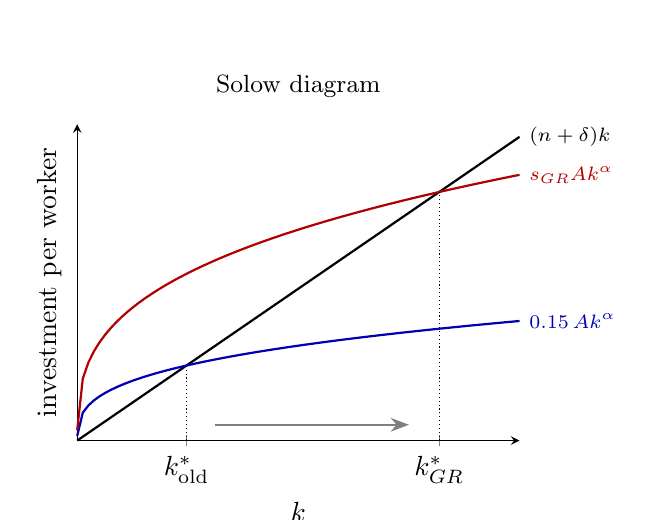
\begin{tikzpicture}
\begin{axis}[width=7.2cm,height=5.6cm,axis lines=left,xmin=0,xmax=16,ymin=0,ymax=1.0,
  xlabel={$k$},ylabel={investment per worker},xtick={3.953,13.095},xticklabels={$k^*_{\text{old}}$,$k^*_{GR}$},
  ytick=\empty,title={\small Solow diagram},clip=false]
\addplot[thick,black,domain=0:16,samples=60]{0.06*x};
\addplot[thick,blue!70!black,domain=0.001:16,samples=80]{0.15*x^(1/3)};
\addplot[thick,red!70!black,domain=0.001:16,samples=80]{(1/3)*x^(1/3)};
\addplot[densely dotted] coordinates {(3.953,0) (3.953,0.2372)};
\addplot[densely dotted] coordinates {(13.095,0) (13.095,0.7857)};
\node[font=\scriptsize,anchor=west] at (axis cs:16,0.96) {$(n+\delta)k$};
\node[font=\scriptsize,blue!70!black,anchor=west] at (axis cs:16,0.378) {$0.15\,Ak^{\alpha}$};
\node[font=\scriptsize,red!70!black,anchor=west] at (axis cs:16,0.84) {$s_{GR}Ak^{\alpha}$};
\draw[-{Stealth},thick,gray] (axis cs:5,0.05)--(axis cs:12,0.05);
\end{axis}
\end{tikzpicture}\quad
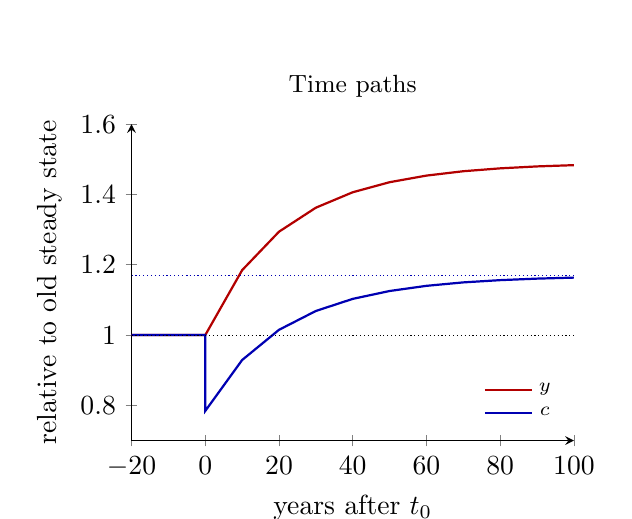
\begin{tikzpicture}
\begin{axis}[width=7.2cm,height=5.6cm,axis lines=left,xmin=-20,xmax=100,ymin=0.7,ymax=1.6,
  xlabel={years after $t_0$},ylabel={relative to old steady state},title={\small Time paths},
  legend style={font=\scriptsize,draw=none,at={(0.98,0.03)},anchor=south east}]
\addplot[thick,red!70!black] coordinates {(-20,1) (0,1) (10,1.1847) (20,1.2941) (30,1.3624) (40,1.4063)
  (50,1.4349) (60,1.4537) (70,1.4661) (80,1.4743) (90,1.4798) (100,1.4834)};
\addplot[thick,blue!70!black] coordinates {(-20,1) (0,1) (0,0.7843) (10,0.9291) (20,1.0150) (30,1.0686)
  (40,1.1030) (50,1.1254) (60,1.1401) (70,1.1499) (80,1.1563) (90,1.1606) (100,1.1635)};
\addplot[densely dotted,domain=-20:100]{1};
\addplot[densely dotted,blue!70!black,domain=-20:100]{1.1692};
\legend{$y$,$c$}
\end{axis}
\end{tikzpicture}
\end{center}
\passo{6 --- welfare}{Not necessarily. Brazil starts \emph{below} the golden rule ($0.15<1/3$), so the economy
is dynamically efficient and more steady-state consumption must be bought with less consumption during the
transition: current workers and retirees pay (21.6\% less consumption at once, below the old level for 18
years); later cohorts gain. Whether it is worth it depends on how the future is discounted --- an impatient
society optimally stays below $s_{GR}$ (compare optimal and fixed saving rates, Kurlat ex.~9.12, p.~185).
Only from \emph{above} $s_{GR}$ would a change (a cut in $s$) raise consumption at every date, a Pareto
improvement.}
\intuicao{A higher saving rate keeps raising output, but each extra unit of capital also needs $n+\delta$ of
replacement; past the point where MPK $=n+\delta$, capital costs more to maintain than it adds. With
Cobb--Douglas that point is reached exactly when the saving rate equals capital's income share.}
\refbib{Kurlat ch.~4, \S4.2 (steady state, pp.~59--61) and \S4.3 (golden rule, pp.~61--63); Jones (2020) ch.~5
for the transition paths.}
\rubrica{
\item (i) $k^*$ and $c^*$ with the exponent $\alpha/(1-\alpha)$: 0.15; $s_{GR}=\alpha$ derived: 0.1; MPK
cross-check: 0.1. Dropping the exponent (answer other than $\alpha$): max.\ 0.15 on (i). Maximising $k^*$ or
$y^*$ instead of $c^*$: 0 on (i).
\item (ii) Impact $-21.6\%$ with the reason (predetermined $k$): 0.1; $+16.9\%$ and $+49.1\%$: 0.15 (slip:
$-0.1$). Consumption rising on impact: 0 on that line.
\item (iii) Solow diagram with both curves and both crossings labelled: 0.1; time paths, $c$ jumping down and
$y$ not jumping: 0.1.
\item (iv) Trade-off and who pays: 0.1; why only above $s_{GR}$ is a change Pareto improving: 0.1.
}
\gap{Prova 01, 1.b--1.c (three approaches with all entries; what counts as investment) and 2.b (golden-rule
algebra: carry the exponent, cross-check with MPK $=n+\delta$).}
\end{sol}

% =============================================================================
\questao{(2.5 points) A labour tax: what it does depends on what the government does with the money.
\textnormal{\normalsize A one-period economy has a fixed capital stock $\bar K$, owned by the representative
household, which also owns the competitive firm. The household has one unit of time and utility
\eqref{q2:U}, with $\psi=1/3$. The firm produces \eqref{q2:F} with $\alpha=1/3$;
normalise $A\bar K^{\alpha}=1$. Labour income is taxed at rate $\tau$, so the household's budget is
\eqref{q2:BC}, where $T$ is a lump-sum transfer that the household takes as given:
\begin{align}
u &= \ln c+\psi\ln(1-L), \tag{U}\label{q2:U}\\
Y &= A\bar K^{\alpha}L^{1-\alpha}, \tag{F}\label{q2:F}\\
c &= (1-\tau)wL+r\bar K+\Pi+T. \tag{BC}\label{q2:BC}
\end{align}
Congress debates a 25\% tax on labour income.}}

\parte{a}{0.7 point} Let $\tau=T=0$. Write the household's and the firm's problems, their first-order
conditions and the market-clearing conditions; show that profits are zero, and find the equilibrium $L$, $Y$,
$w$ and $c$. Then solve the problem of a planner who chooses $c$ and $L$ subject only to technology, and show that
it gives the same allocation. State the theorem behind this and the assumptions it needs.
\resolespaco
\begin{sol}
\begin{notacao}
\item $c\ge0$: consumption. $L\in[0,1]$: hours worked; $1-L$: leisure (one unit of time).
\item $\psi>0$: weight of leisure in utility ($\psi=1/3$).
\item $Y$: output. $\bar K>0$: fixed capital stock. $A>0$: productivity, with $A\bar K^{\alpha}=1$.
$\alpha\in(0,1)$: capital's share ($\alpha=1/3$).
\item $w$, $r>0$: real wage and real rental rate of capital. $\Pi$: the firm's profit, paid to the household.
\item $\tau\in[0,1)$: tax rate on labour income. $T$: lump-sum transfer. In this item $\tau=T=0$.
\item $L_0$, $Y_0$, $w_0$, $c_0$: the equilibrium at $\tau=0$. $L^{P}$: the planner's choice.
\item MRS: marginal rate of substitution of leisure for consumption. MPL: marginal product of labour.
\end{notacao}
\passo{1 --- household}{With $\tau=T=0$, \eqref{q2:BC} is
\begin{equation}
c=wL+r\bar K+\Pi. \label{q2a:bc}
\end{equation}
Substitute \eqref{q2a:bc} into \eqref{q2:U}:
\[
\max_L\ \ln(wL+r\bar K+\Pi)+\psi\ln(1-L).
\]
Differentiate with respect to $L$ and set it to zero:
\[
\frac{w}{c}-\frac{\psi}{1-L}=0.
\]
Rearrange:
\begin{equation}
\boxed{\frac{\psi c}{1-L}=w} \label{q2a:hh}
\end{equation}
--- the marginal rate of substitution between leisure and consumption equals the real wage, the price of
leisure.}
\passo{2 --- firm}{The firm chooses $L$ and rents $\bar K$:
$\max\ A\bar K^{\alpha}L^{1-\alpha}-wL-r\bar K$. Differentiating \eqref{q2:F}:
\begin{align}
w &= (1-\alpha)A\bar K^{\alpha}L^{-\alpha}\nonumber\\
&= \frac{(1-\alpha)\big(A\bar K^{\alpha}L^{1-\alpha}\big)}{L}\nonumber\\
&= \frac{(1-\alpha)Y}{L}, \label{q2a:w}\\
r &= \alpha A\bar K^{\alpha-1}L^{1-\alpha}\nonumber\\
&= \frac{\alpha\big(A\bar K^{\alpha}L^{1-\alpha}\big)}{\bar K}\nonumber\\
&= \frac{\alpha Y}{\bar K}. \label{q2a:r}
\end{align}
Profits, using \eqref{q2a:w} and \eqref{q2a:r}:
\begin{align}
\Pi &= Y-wL-r\bar K\nonumber\\
&= Y-\left(\frac{(1-\alpha)Y}{L}\right)L-\left(\frac{\alpha Y}{\bar K}\right)\bar K\nonumber\\
&= Y-(1-\alpha)Y-\alpha Y\nonumber\\
&= \boxed{0} \label{q2a:pi}
\end{align}
(constant returns: factor payments exhaust output).}
\passo{3 --- clearing}{Labour: household supply $=$ firm demand; capital: $\bar K$; goods (no $G$):
\begin{equation}
c=Y. \label{q2a:goods}
\end{equation}}
\passo{4 --- solve}{Substitute \eqref{q2a:goods} and \eqref{q2a:w} into \eqref{q2a:hh}:
\begin{align*}
\frac{\psi\,(Y)}{1-L} &= \left(\frac{(1-\alpha)Y}{L}\right)\\
\psi L &= (1-\alpha)(1-L)\\
(1-\alpha+\psi)L &= 1-\alpha.
\end{align*}
Hence
\begin{align}
L_0 &= \boxed{\frac{1-\alpha}{1-\alpha+\psi}}\nonumber\\
&= \frac{1-\frac13}{1-\frac13+\frac13}\nonumber\\
&= \frac{2/3}{1}=\boxed{\tfrac23}. \label{q2a:L0}
\end{align}
Then, by \eqref{q2:F} with $A\bar K^{\alpha}=1$, \eqref{q2a:w}, \eqref{q2a:goods} and \eqref{q2a:r}:
\begin{align*}
Y_0 &= (2/3)^{2/3}=0.7631,\\
w_0 &= \frac{(2/3)(0.7631)}{2/3}=0.7631,\\
c_0 &= Y_0=0.7631,\\
r\bar K &= \alpha Y_0=\tfrac13(0.7631)=0.2544.
\end{align*}}
\passo{5 --- planner}{The planner substitutes technology \eqref{q2:F} into \eqref{q2:U}:
\begin{align}
\max_L\ \ln\!\big(A\bar K^{\alpha}L^{1-\alpha}\big)+\psi\ln(1-L)
=\text{const}+(1-\alpha)\ln L+\psi\ln(1-L). \label{q2a:plan}
\end{align}
Differentiate \eqref{q2a:plan} with respect to $L$:
\begin{equation}
\frac{1-\alpha}{L}=\frac{\psi}{1-L}. \label{q2a:planfoc}
\end{equation}
Cross-multiplying \eqref{q2a:planfoc} gives the second line of Step 4, so $L^{P}=\tfrac23$ (SOC: both terms
concave). The planner sets MRS $=$ MPL; the market sets MRS $=w$ \eqref{q2a:hh} and MPL $=w$ \eqref{q2a:w},
hence MRS $=$ MPL.}
\passo{6 --- theorem}{\textbf{First Welfare Theorem}: a competitive equilibrium is Pareto efficient, given
price-taking agents, complete markets, no externalities and no distortionary taxes. Here all hold at $\tau=0$.}
\refbib{Kurlat ch.~9, \S9.1--\S9.2, pp.~165--172 (equilibrium and the First Welfare Theorem); ch.~7, \S7.2,
pp.~131--137 (consumption--leisure choice).}
\rubrica{
\item Household FOC (MRS $=w$) and firm FOCs: 0.2. $\Pi=0$ shown: 0.1. Clearing conditions listed: 0.1.
\item $L_0=2/3$ with $Y,w,c$: 0.1 (slip: $-0.1$).
\item Planner's FOC and same allocation: 0.1. Theorem and its assumptions: 0.1.
\item Omitting capital income or profits from the budget: max.\ 0.4 on the item.
}
\end{sol}

\parte{b}{0.7 point} Now $\tau=25\%$ and the government returns the whole revenue as the transfer, so
$T=\tau wL$ in equilibrium. Find $L$ (in general and in numbers). Explain why returning the money does not undo
the effect of the tax. Show graphically, in the plane (leisure $\ell=1-L$, consumption $c$): the production
possibilities frontier, the equilibrium of (a), the new equilibrium, and the household's budget line at the new
equilibrium, with and without the transfer. Use the graph to explain why the new allocation is inefficient.
\resolespaco
\begin{sol}
\begin{notacao}
\item Symbols of (a) keep their meaning. New here:
\item $\tau=0.25$; $T=\tau wL$: the rebate, equal to the revenue in equilibrium, taken as given by the household.
\item $L_R$: hours under the rebated tax. $\ell\equiv1-L\in[0,1]$: leisure; $\ell_0$, $\ell_R$ at the two equilibria.
\item $E_0$, $E_R$: the equilibria of (a) and (b). $U_0$, $U_R$: the indifference curves through them.
\end{notacao}
\passo{1 --- FOC with the tax}{Substitute \eqref{q2:BC} into \eqref{q2:U}:
\[
\max_L\ \ln\big((1-\tau)wL+r\bar K+\Pi+T\big)+\psi\ln(1-L).
\]
Differentiate with respect to $L$, with $T$ taken as given, and set it to zero:
\[
\frac{(1-\tau)w}{c}-\frac{\psi}{1-L}=0.
\]
Rearrange, as in (a), now with $(1-\tau)w$ per hour:
\begin{equation}
\boxed{\frac{\psi c}{1-L}=(1-\tau)w}. \label{q2b:hh}
\end{equation}
$T$ does not appear: the household takes it as given, so it moves income, not the price of leisure.}
\passo{2 --- equilibrium}{The government returns the revenue:
\begin{equation}
T=\tau wL. \label{q2b:gov}
\end{equation}
Substitute \eqref{q2b:gov} into \eqref{q2:BC}, with $\Pi=0$ from \eqref{q2a:pi}, and then use \eqref{q2a:w} and
\eqref{q2a:r}:
\begin{align}
c &= (1-\tau)wL+r\bar K+(0)+(\tau wL)\nonumber\\
&= wL+r\bar K\nonumber\\
&= \left(\frac{(1-\alpha)Y}{L}\right)L+\left(\frac{\alpha Y}{\bar K}\right)\bar K\nonumber\\
&= (1-\alpha)Y+\alpha Y\nonumber\\
&= Y. \label{q2b:cY}
\end{align}
Substitute \eqref{q2b:cY} and \eqref{q2a:w} into \eqref{q2b:hh}:
\begin{align*}
\frac{\psi\,(Y)}{1-L} &= (1-\tau)\left(\frac{(1-\alpha)Y}{L}\right)\\
\psi L &= (1-\tau)(1-\alpha)(1-L).
\end{align*}
Solve for $L$:
\begin{equation}
\boxed{L_R=\frac{(1-\tau)(1-\alpha)}{\psi+(1-\tau)(1-\alpha)}}. \label{q2b:LR}
\end{equation}
Numbers: $(1-\tau)(1-\alpha)=0.75\cdot\tfrac23=0.5$, so
\[
L_R=\frac{0.5}{\frac13+0.5}=\frac{0.5}{0.8333}=\boxed{0.60}.
\]
Sign, differentiating \eqref{q2b:LR}:
\[
\frac{\partial L_R}{\partial\tau}=-\frac{\psi(1-\alpha)}{[\psi+(1-\tau)(1-\alpha)]^2}<0.
\]
The other variables, by \eqref{q2:F}, \eqref{q2a:w}, \eqref{q2b:gov}, \eqref{q2a:r} and \eqref{q2b:cY}:
\begin{align*}
Y &= 0.6^{2/3}=0.7114,\\
w &= \frac{(2/3)(0.7114)}{0.6}=0.7904,\\
(1-\tau)w &= 0.75(0.7904)=0.5928,\\
T &= 0.25(0.7904)(0.6)=0.1186=\tau(1-\alpha)Y,\\
r\bar K &= \alpha Y=\tfrac13(0.7114)=0.2371,\\
c &= Y=0.7114.
\end{align*}}
\passo{3 --- why the rebate does not undo it}{Each household compares one more hour with $(1-\tau)w$, not
with $w$: its own extra hour raises the transfer to \emph{everyone} by a negligible amount, so it ignores it.
In equilibrium the transfer returns the \emph{income} (\eqref{q2b:cY}: $c=Y$ exactly) but the \emph{price} of
leisure stays distorted. Combining \eqref{q2b:hh} with $w=\text{MPL}$ from \eqref{q2a:w}:
\#~a wedge, $\text{MRS}=(1-\tau)\,\text{MPL}<\text{MPL}$.}
\begin{center}
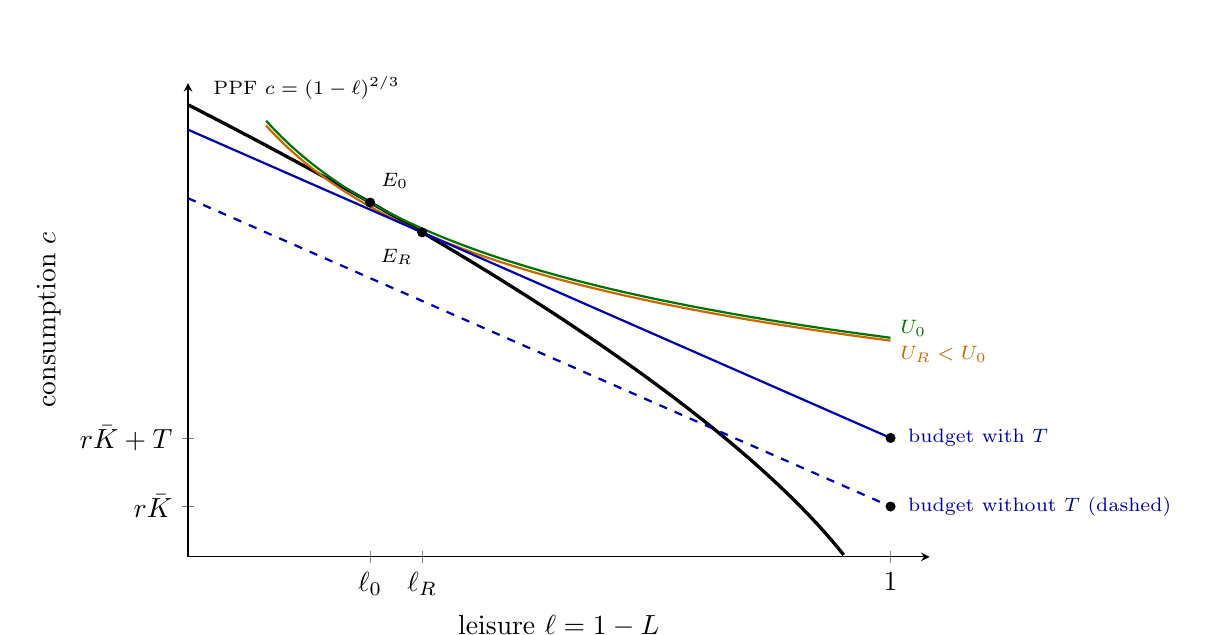
\begin{tikzpicture}
\begin{axis}[width=11cm,height=7.6cm,axis lines=left,xmin=0.1,xmax=1.05,ymin=0.15,ymax=0.97,clip=false,
  xlabel={leisure $\ell=1-L$},ylabel={consumption $c$},xtick={0.3333,0.4,1},xticklabels={$\ell_0$,$\ell_R$,$1$},
  ytick={0.2371,0.3557},yticklabels={$r\bar K$,$r\bar K+T$}]
\addplot[very thick,black,domain=0.1:0.94,samples=120]{(1-x)^(2/3)};
\addplot[thick,green!45!black,domain=0.2:1,samples=80]{0.52912*x^(-1/3)};
\addplot[thick,orange!80!black,domain=0.2:1,samples=80]{0.52418*x^(-1/3)};
\addplot[thick,blue!70!black,domain=0.1:1]{0.3557+0.5928*(1-x)};
\addplot[thick,blue!70!black,dashed,domain=0.1:1]{0.2371+0.5928*(1-x)};
\addplot[only marks,mark=*,mark size=1.6pt] coordinates {(0.3333,0.7631) (0.4,0.7114) (1,0.3557) (1,0.2371)};
\node[font=\scriptsize,anchor=south west] at (axis cs:0.335,0.77) {$E_0$};
\node[font=\scriptsize,anchor=north east] at (axis cs:0.40,0.70) {$E_R$};
\node[font=\scriptsize,anchor=south west] at (axis cs:0.12,0.925) {PPF $c=(1-\ell)^{2/3}$};
\node[font=\scriptsize,green!45!black,anchor=west] at (axis cs:1,0.545) {$U_0$};
\node[font=\scriptsize,orange!80!black,anchor=west] at (axis cs:1,0.50) {$U_R<U_0$};
\node[font=\scriptsize,blue!70!black,anchor=west] at (axis cs:1.01,0.3557) {budget with $T$};
\node[font=\scriptsize,blue!70!black,anchor=west] at (axis cs:1.01,0.2371) {budget without $T$ (dashed)};
\end{axis}
\end{tikzpicture}\\
{\footnotesize $E_0$: the indifference curve $U_0$ is tangent to the frontier (MRS $=$ MPL). $E_R$: the household is
tangent to its after-tax budget line (slope $(1-\tau)w=0.59$), which is flatter than the frontier there
(MPL $=w=0.79$), so the frontier \emph{crosses} $U_R$: there are feasible points above $U_R$. The tax rotates the
budget line about the no-work point $(1,r\bar K)$; the transfer shifts it up in parallel by $T$.}
\end{center}
\intuicao{The rebate gives the money back, but not the incentive: households still see 75 centavos for every real
their hour produces, so they buy too much leisure.}
\refbib{Kurlat ch.~7, \S7.2 (taxes and labour supply), pp.~131--137; related, not the same: ex.~7.5
\emph{Prescott's Calculation}, p.~148; ch.~9, \S9.2.}
\rubrica{
\item FOC with $(1-\tau)w$ and $c=Y$ from the government budget: 0.2. $L_R=0.6$ with the general formula and its
sign: 0.15 (slip: $-0.1$).
\item Why the transfer does not undo the wedge: 0.15. Claiming the rebate makes the tax neutral: max.\ 0.3 on the item.
\item Graph: axes, frontier, two indifference curves, tangency at $E_0$: 0.1; budget line rotated about the
no-work point and shifted by $T$, crossing argument at $E_R$: 0.1. Shifting the budget parallel for the tax: $-0.1$.
}
\end{sol}

\parte{c}{0.6 point} Instead, the same 25\% tax finances government purchases $G=\tau wL$ that give households
no utility ($T=0$). Find $L$. Using (a) and (b), split the change in hours relative to $\tau=0$ into a substitution
effect and an income effect, and explain why hours fall less than in (b). What happens if $\alpha=0$? An economist
argues: ``Labour taxes spent by the government barely change hours, so they cause almost no distortion.''
Evaluate, comparing with financing the same $G$ through a lump-sum tax.
\resolespaco
\begin{sol}
\begin{notacao}
\item Symbols of (a)--(b) keep their meaning. New here:
\item $G=\tau wL\ge0$: government purchases, which give no utility; now $T=0$.
\item $L_G$: hours when the tax finances $G$.
\item Substitution effect: change in $L$ from a change in the after-tax wage with income held fixed;
income effect: change in $L$ from the change in income alone.
\end{notacao}
\passo{1 --- equilibrium}{With $T=0$ and $\Pi=0$ \eqref{q2a:pi}, \eqref{q2:BC} becomes, using $wL+r\bar K=Y$
(Step 2 of (b)) and $wL=(1-\alpha)Y$ from \eqref{q2a:w}:
\begin{align}
c &= (1-\tau)wL+r\bar K+(0)+(0)\nonumber\\
&= (wL+r\bar K)-\tau wL\nonumber\\
&= (Y)-\tau wL\nonumber\\
&= Y-\tau\big((1-\alpha)Y\big)\nonumber\\
&= Y\,[1-\tau(1-\alpha)]. \label{q2c:c}
\end{align}
Numbers: $1-0.25\cdot\tfrac23=\tfrac56$, so $c=\tfrac56Y$ (goods clearing $c+G=Y$ gives the same).
The FOC \eqref{q2b:hh} still holds. Substitute \eqref{q2c:c} and \eqref{q2a:w} into it:
\begin{align*}
\frac{\psi\,\big([1-\tau(1-\alpha)]Y\big)}{1-L} &= (1-\tau)\left(\frac{(1-\alpha)Y}{L}\right)\\
\psi[1-\tau(1-\alpha)]\,L &= (1-\tau)(1-\alpha)(1-L).
\end{align*}
Solve for $L$:
\begin{equation}
\boxed{L_G=\frac{(1-\tau)(1-\alpha)}{\psi[1-\tau(1-\alpha)]+(1-\tau)(1-\alpha)}}. \label{q2c:LG}
\end{equation}
Numbers: $\psi[1-\tau(1-\alpha)]=\tfrac13\cdot\tfrac56=\tfrac{5}{18}$ and $(1-\tau)(1-\alpha)=0.5=\tfrac{9}{18}$:
\[
L_G=\frac{9/18}{\frac{5}{18}+\frac{9}{18}}=\boxed{\tfrac{9}{14}=0.643}.
\]
Then, by \eqref{q2:F}, \eqref{q2a:w} and \eqref{q2c:c}:
\begin{align*}
Y &= (9/14)^{2/3}=0.7449,\\
G &= \tau(1-\alpha)Y=\tfrac16(0.7449)=0.1241,\\
c &= \tfrac56(0.7449)=0.6207.
\end{align*}}
\passo{2 --- decomposition}{(b) changes the price of leisure but gives the income back: it isolates the
\textbf{substitution effect}. From \eqref{q2b:LR} and \eqref{q2a:L0}:
\[
L_R-L_0=0.600-0.667=\boxed{-0.067}.
\]
(c) has the same price change and also takes the income away: the step from (b) to (c) is the
\textbf{income effect}. From \eqref{q2c:LG} and \eqref{q2b:LR}:
\[
L_G-L_R=0.643-0.600=\boxed{+0.043}
\]
(poorer households buy less leisure, a normal good). Total:
\[
L_G-L_0=0.643-0.667=\boxed{-0.024}.
\]}
\passo{3 --- why less, and $\alpha=0$}{The two effects have opposite signs. With log utility they cancel only if
all income is taxed labour income. Here capital income $r\bar K$ is untaxed, so the income loss is smaller than
the price change: substitution wins and hours fall, but by less. Set $\alpha=0$ in \eqref{q2c:LG}:
\begin{align*}
L_G &= \frac{(1-\tau)(1-0)}{\psi[1-\tau(1-0)]+(1-\tau)(1-0)}\\
&= \frac{1-\tau}{\psi(1-\tau)+(1-\tau)}\\
&= \frac{1}{1+\psi},
\end{align*}
\textbf{independent of $\tau$}: exact cancellation.}
\passo{4 --- the economist}{Wrong. The distortion is the wedge MRS $=(1-\tau)$MPL, and its cost is driven by the
\emph{substitution} effect, not by the total response of hours. Benchmark: the same $G=0.1241$ raised lump-sum
leaves MRS $=$ MPL, so \eqref{q2a:hh} with $c=Y-G$ and \eqref{q2a:w} give
\begin{equation}
\frac{\psi(Y-G)}{1-L}=\frac{(1-\alpha)Y}{L}. \label{q2c:ls}
\end{equation}
Solving \eqref{q2c:ls} numerically gives $L=0.703$, more hours than at $\tau=0$ (pure income effect), and higher
utility: $-0.8104$ vs $-0.8201$, a consumption-equivalent gap of about $1.0\%$. Hours barely move under the
labour tax because two effects offset, not because nothing is distorted.}
\intuicao{The observer sees the total change in hours; welfare depends on the compensated change. A tax can leave
hours almost unchanged and still be costly, because it is the gap between what an hour produces and what it pays
that wastes resources.}
\refbib{Kurlat ch.~7, \S7.2 (income and substitution effects; log case), pp.~131--137; ch.~9, \S9.2.}
\rubrica{
\item $L_G=9/14$ with $c=Y[1-\tau(1-\alpha)]$: 0.2 (slip: $-0.1$).
\item Decomposition with signs and the reason (each effect named): 0.15. Reversing the labels: max.\ 0.1 on this line.
\item Why smaller here and the $\alpha=0$ case: 0.1.
\item Economist: wedge and compensated effect, with the lump-sum benchmark: 0.15. Conceding the claim: 0 on this line.
}
\end{sol}

\parte{d}{0.5 point} Return to the rebated tax of (b). Compute the welfare cost of the 25\% tax as the
percentage increase in consumption, at the allocation of (b), that would give households the utility of (a).
Show that the cost is of second order in $\tau$ (that a small tax has a much smaller cost) and check it with
$\tau=12.5\%$. Which instrument would avoid the cost?
\resolespaco
\begin{sol}
\begin{notacao}
\item Symbols of (a)--(b) keep their meaning. New here:
\item $U(L)$: utility as a function of hours when $c=Y$. $U_0$, $U_R$: its values in (a) and (b).
\item $\lambda\ge0$: welfare cost, the proportional rise in consumption at the allocation of (b) that gives
utility $U_0$.
\item $L_R(\tau)$: hours under the rebated tax as a function of $\tau$, from \eqref{q2b:LR}.
\end{notacao}
\passo{1 --- utility}{In both economies $c=Y$ (\eqref{q2a:goods}, \eqref{q2b:cY}) and, by \eqref{q2:F} with
$A\bar K^{\alpha}=1$, $Y=L^{2/3}$. Substitute into \eqref{q2:U}:
\begin{align}
U(L) &= \ln\big(L^{2/3}\big)+\tfrac13\ln(1-L)\nonumber\\
&= \tfrac23\ln L+\tfrac13\ln(1-L). \label{q2d:U}
\end{align}
Evaluate \eqref{q2d:U} at $L_0=\tfrac23$ and $L_R=0.6$:
\begin{align*}
U_0 &= \tfrac23\ln\tfrac23+\tfrac13\ln\tfrac13\\
&= (-0.27031)+(-0.36620)\\
&= -0.63651,\\
U_R &= \tfrac23\ln0.6+\tfrac13\ln0.4\\
&= (-0.34055)+(-0.30543)\\
&= -0.64598.
\end{align*}}
\passo{2 --- consumption equivalent}{By definition of $\lambda$:
\begin{equation}
\ln\big((1+\lambda)c_R\big)+\psi\ln(1-L_R)=U_0. \label{q2d:lam}
\end{equation}
Split the log in \eqref{q2d:lam} and use $U_R=\ln c_R+\psi\ln(1-L_R)$:
\begin{align*}
\ln(1+\lambda)+\big(\ln c_R+\psi\ln(1-L_R)\big) &= U_0\\
\ln(1+\lambda)+(U_R) &= U_0\\
\ln(1+\lambda) &= U_0-U_R\\
&= (-0.63651)-(-0.64598)\\
&= 0.00947,
\end{align*}
and $\lambda=e^{(0.00947)}-1=\boxed{0.95\%}$ of consumption.}
\passo{3 --- second order}{Welfare as a function of the tax is
\begin{equation}
U(\tau)=U\big(L_R(\tau)\big). \label{q2d:Utau}
\end{equation}
$L_0=L_R(0)$ maximises \eqref{q2d:U}: it is the planner's problem \eqref{q2a:plan}. Differentiate
\eqref{q2d:Utau} at $\tau=0$:
\begin{align*}
\frac{dU}{d\tau}\Big|_{\tau=0} &= U'(L_0)\,L_R'(0)\\
&= (0)\cdot L_R'(0)=0
\end{align*}
(envelope argument). The first-order term vanishes, and a second-order expansion of \eqref{q2d:Utau} leaves
\begin{equation}
U_0-U(\tau)\approx\tfrac12|U''(L_0)|\,[L_R'(0)]^2\tau^2, \label{q2d:harb}
\end{equation}
the Harberger triangle. Check: at $\tau=12.5\%$ the cost is $0.20\%$, about a fifth of $0.95\%$, close to the
quarter that \eqref{q2d:harb} predicts (the rest is higher-order terms).}
\passo{4 --- instrument}{A lump-sum tax (here, simply not taxing and not transferring): it does not touch the
marginal trade-off, so MRS $=$ MPL holds and the First Welfare Theorem applies again.}
\intuicao{At the efficient point the first hour moved has no value, so a small wedge costs almost nothing; the cost
grows with the square of the wedge, which is why many small taxes beat one large one.}
\refbib{Kurlat ch.~9, \S9.2 (welfare and taxes), pp.~168--172; ch.~7, \S7.2.}
\rubrica{
\item $U_0$, $U_R$ and $\lambda=0.95\%$: 0.2 (slip: $-0.1$). Comparing utils without converting: max.\ 0.1 on this line.
\item Envelope argument for the second-order cost: 0.15; $\tau=12.5\%$ check: 0.05.
\item Lump-sum tax as the first-best instrument: 0.1.
}
\gap{Kurlat ch.~7 and ch.~9 were absent from Prova 01; Prova 01, 2.c--2.d (list every income source, including
capital income and profits, and every choice variable).}
\end{sol}

% =============================================================================
\questao{(2.5 points) The Real plan, the trip to the bank and the inflation tax.
A stylised Brazil in the early 1990s. A representative household spends its real income $Y$ per year at a constant
rate. It keeps its wealth in an account that pays the nominal rate $i$ and withdraws cash $N$ times a year, in equal
amounts; cash pays no interest. Each trip to the bank costs $F$ in goods (queue, fee, time), that is $pF$ in money.
Take $Y=60{,}000$ (reais of constant purchasing power per year) and $F=25$. In the long run real output grows at
$g=4\%$ a year, the real interest rate is $r=3\%$ and the money supply grows at $\mu=11\%$ a year. Treat all money
as currency (money multiplier equal to one) and use Kurlat's Fisher equation $i=r+\pi$.}

\parte{a}{0.6 point} Derive the optimal number of trips $N$ and the demand for real money balances $M/p$ from the
household's cost minimisation. Find the income and interest elasticities of money demand and the velocity of
money. Compute $N$, $M/p$ and velocity at $i=12\%$. Show graphically how money demand depends on $i$, and how a
fall in $F$ (more ATMs) moves it.
\resolespaco
\begin{sol}
\begin{notacao}
\item $Y>0$: real income per year, spent at a constant rate ($Y=60{,}000$). $p>0$: price level.
\item $i>0$: nominal interest rate on the account; cash pays nothing.
\item $N>0$: withdrawals per year (an integer $\ge1$ in practice); $N^*$ the optimum.
\item $F>0$: real cost of one trip to the bank ($F=25$), so $pF$ in money.
\item $M$: average nominal cash held; $m\equiv M/p$: real money balances.
\item $\mathcal C(N)$: annual nominal cost of managing cash.
\item $\eta$: income elasticity of money demand. $V$: velocity of money.
\end{notacao}
\passo{1 --- the costs}{Each withdrawal is $pY/N$, spent at a constant rate down to zero, so average cash is
half of it:
\begin{equation}
M=\frac{pY}{2N}. \label{q3a:M}
\end{equation}
Annual cost: forgone interest on that cash plus the trips:
\begin{equation}
\mathcal C(N)=\frac{i\,pY}{2N}+pFN. \label{q3a:cost}
\end{equation}}
\passo{2 --- FOC}{Differentiate \eqref{q3a:cost} with respect to $N$ and set it to zero:
\begin{equation}
\mathcal C'(N)=-\frac{ipY}{2N^2}+pF=0. \label{q3a:foc}
\end{equation}
Solve \eqref{q3a:foc} for $N$:
\begin{equation}
\boxed{N^*=\sqrt{\frac{iY}{2F}}} \label{q3a:N}
\end{equation}
(SOC: $\mathcal C''=ipY/N^3>0$). Divide \eqref{q3a:M} by $p$ and substitute \eqref{q3a:N}:
\begin{align}
\frac{M}{p} &= \frac{Y}{2N^*}\nonumber\\
&= \frac{Y}{2\left(\sqrt{\frac{iY}{2F}}\right)}\nonumber\\
&= \frac{Y}{2}\sqrt{\frac{2F}{iY}}\nonumber\\
&= \sqrt{\frac{FY}{2i}}. \label{q3a:md}
\end{align}}
\passo{3 --- elasticities and velocity}{Take the log of \eqref{q3a:md}:
\begin{equation}
\ln\frac Mp=\tfrac12\ln\frac F2+\tfrac12\ln Y-\tfrac12\ln i. \label{q3a:ln}
\end{equation}
The coefficients in \eqref{q3a:ln} are the elasticities: income elasticity $\boxed{\eta=\tfrac12}$, interest
elasticity $\boxed{-\tfrac12}$ (economies of scale in cash management). Velocity, using the first line of
\eqref{q3a:md} and then \eqref{q3a:N}:
\begin{align}
V\equiv\frac{pY}{M} &= \frac{Y}{M/p}\nonumber\\
&= \frac{Y}{\left(\frac{Y}{2N^*}\right)}\nonumber\\
&= 2N^*\nonumber\\
&= 2\left(\sqrt{\frac{iY}{2F}}\right)\nonumber\\
&= \sqrt{\frac{2iY}{F}}: \label{q3a:V}
\end{align}
not a constant; it rises with $i$ and $Y$.}
\passo{4 --- numbers}{At $i=0.12$, by \eqref{q3a:N}, \eqref{q3a:md} and \eqref{q3a:V}:
\begin{align*}
N^* &= \sqrt{\frac{0.12\cdot60{,}000}{2\cdot25}}=\sqrt{144}=\boxed{12}\ \text{trips a year},\\
\frac Mp &= \frac{60{,}000}{2\cdot12}=\frac{60{,}000}{24}=\boxed{2{,}500},\\
V &= 2\cdot12=\boxed{24}.
\end{align*}}
\begin{center}
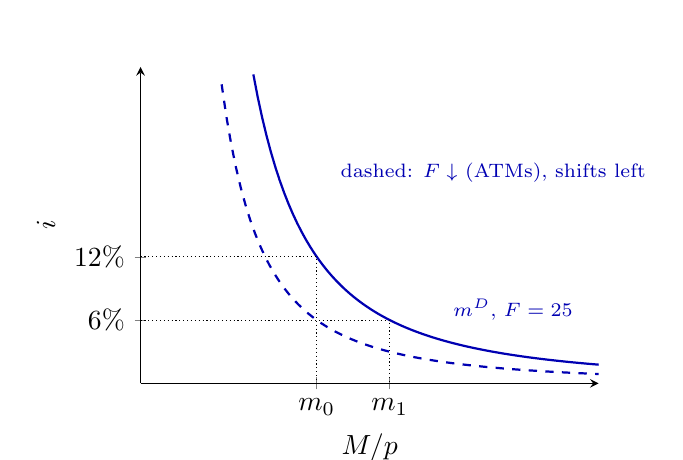
\begin{tikzpicture}
\begin{axis}[width=7.4cm,height=5.6cm,axis lines=left,xmin=0,xmax=6500,ymin=0,ymax=0.3,
  xlabel={$M/p$},ylabel={$i$},xtick={2500,3535.5},xticklabels={$m_0$,$m_1$},ytick={0.06,0.12},
  yticklabels={6\%,12\%},scaled x ticks=false,clip=false]
\addplot[thick,blue!70!black,domain=1600:6500,samples=80]{750000/x^2};
\addplot[thick,blue!70!black,dashed,domain=1150:6500,samples=80]{375000/x^2};
\addplot[densely dotted] coordinates {(0,0.12) (2500,0.12) (2500,0)};
\addplot[densely dotted] coordinates {(0,0.06) (3535.5,0.06) (3535.5,0)};
\node[font=\scriptsize,blue!70!black,anchor=west] at (axis cs:4300,0.07) {$m^D$, $F=25$};
\node[font=\scriptsize,blue!70!black,anchor=west] at (axis cs:2700,0.2) {dashed: $F\downarrow$ (ATMs), shifts left};
\end{axis}
\end{tikzpicture}
\end{center}
{\footnotesize Downward-sloping in $i$ (elasticity $-\tfrac12$); a lower $F$ shifts the whole curve left
(fewer balances at every $i$). Points used in (b): $i=12\%$ and $6\%$.}
\intuicao{Holding cash costs interest; refilling it costs trips. Doubling spending does not double cash, because the
trip cost is fixed: the optimal number of trips rises too.}
\refbib{Kurlat ch.~10, \S10.4, pp.~199--204, eqs.~(10.4.3)--(10.4.4); the exercise on ATMs, ex.~10.4, p.~203,
is related practice.}
\rubrica{
\item Average cash $pY/2N$ and the cost function: 0.15. $N^*$ and $M/p$ derived: 0.15.
\item Both elasticities and $V=2N$: 0.1. Numbers 12, 2{,}500, 24: 0.1 (slip: $-0.1$).
\item Graph with $i$ and $M/p$ on the axes and the shift for $F\downarrow$: 0.1.
\item Quoting $\sqrt{FY/2i}$ without deriving it: max.\ 0.2 on the item.
}
\end{sol}

\parte{b}{0.7 point} Using money-market equilibrium $M=p\,m^D(Y,i)$, derive the steady-state inflation rate when
$Y$ grows at $g$ and $i$ is constant, and compute $\pi$ and $i$. In mid-1994 the central bank cuts money growth
permanently and credibly to $\mu=5\%$. Find the new $\pi$ and $i$ and the change in real balances. Since the stock
of money does not jump by itself, what must happen to the price level on the day of the reform? Which one-time
change in $M$ would avoid it? Draw $\ln M$ and $\ln p$ around the reform, with that one-time change. A commentator
writes: ``After the Real, M1 rose by tens of percent while inflation collapsed, so money does not cause inflation.''
Evaluate.
\resolespaco
\begin{sol}
\begin{notacao}
\item Symbols of (a) keep their meaning. New here:
\item $m^D(Y,i)$: real money demand, \eqref{q3a:md}. A dot is a time derivative ($\dot M=dM/dt$).
\item $\mu\equiv\dot M/M$: money growth. $\pi\equiv\dot p/p$: inflation. $g\equiv\dot Y/Y$: real growth.
$r$: real interest rate. All per year.
\item $T$: date of the reform. $m_0$, $m_1$: real balances before and after; $p_{\text{old}}$, $p_{\text{new}}$:
price level just before and just after.
\end{notacao}
\passo{1 --- differentiate}{Money-market equilibrium at every date:
\begin{equation}
M_t=p_t\,m^D(Y_t,i_t). \label{q3b:mm}
\end{equation}
Differentiate \eqref{q3b:mm} with respect to $t$:
\begin{equation}
\dot M=\dot p\,m^D+p\Big(\frac{\partial m^D}{\partial Y}\dot Y+\frac{\partial m^D}{\partial i}\dot i\Big).
\label{q3b:diff}
\end{equation}
Set $\dot i=0$ and divide \eqref{q3b:diff} by \eqref{q3b:mm}:
\begin{align}
\frac{\dot M}{M} &= \frac{\dot p\,m^D+p\big(\frac{\partial m^D}{\partial Y}\dot Y+\frac{\partial m^D}{\partial i}(0)\big)}{p\,m^D}
\nonumber\\
&= \frac{\dot p}{p}+\underbrace{\frac{\partial m^D}{\partial Y}\frac{Y}{m^D}}_{\eta}
\frac{\dot Y}{Y}\nonumber\\
\mu &= \pi+\eta g\nonumber\\
\pi &= \mu-\eta g, \label{q3b:pi}
\end{align}
with $\eta=\tfrac12$ from \eqref{q3a:ln}. Kurlat's Fisher equation, from the statement:
\begin{equation}
i=r+\pi. \label{q3b:fisher}
\end{equation}}
\passo{2 --- before}{By \eqref{q3b:pi} and then \eqref{q3b:fisher}:
\begin{align*}
\pi &= 11\%-\tfrac12(4\%)=\boxed{9\%},\\
i &= 3\%+9\%=\boxed{12\%}
\end{align*}
(exact Fisher: $1.03\cdot1.09-1=12.27\%$).}
\passo{3 --- after}{With $\mu=5\%$, by \eqref{q3b:pi} and \eqref{q3b:fisher}:
\begin{align*}
\pi &= 5\%-\tfrac12(4\%)=\boxed{3\%},\\
i &= 3\%+3\%=\boxed{6\%}
\end{align*}
(Fisher effect: $i$ falls one-for-one with $\pi$, $r$ unchanged). Real balances, from the ratio of
\eqref{q3a:md} at the two rates:
\begin{align*}
\frac{m_1}{m_0} &= \frac{\sqrt{FY/(2i_1)}}{\sqrt{FY/(2i_0)}}\\
&= \sqrt{\frac{i_0}{i_1}}\\
&= \sqrt{\frac{0.12}{0.06}}\\
&= \sqrt2=1.414,
\end{align*}
$\boxed{+41.4\%}$ ($2{,}500\to3{,}536$). The jump is immediate: a credible reform changes expected inflation,
hence $i$, at once.}
\passo{4 --- the price level}{Solve \eqref{q3b:mm} for the price level:
\begin{equation}
p=\frac{M}{m^D}. \label{q3b:p}
\end{equation}
If $M$ is continuous and $m^D$ jumps by $\sqrt2$, \eqref{q3b:p} makes $p$ jump \emph{down}:
\begin{align*}
\frac{p_{\text{new}}}{p_{\text{old}}} &= \frac{M/m_1}{M/m_0}\\
&= \frac{m_0}{m_1}\\
&= \frac{1}{\sqrt2}=0.707,
\end{align*}
a $\boxed{29.3\%}$ fall in the price level. To keep $p$ continuous in \eqref{q3b:p}, $M$ must jump with $m^D$:
the central bank issues a one-time injection
\[
\boxed{\frac{\Delta M}{M}=\sqrt2-1=41.4\%}
\]
on the day of the reform (remonetisation), and \emph{from then on} money grows at 5\%. This injection is not
inflationary: it only meets the higher demand for real balances.}
\begin{center}
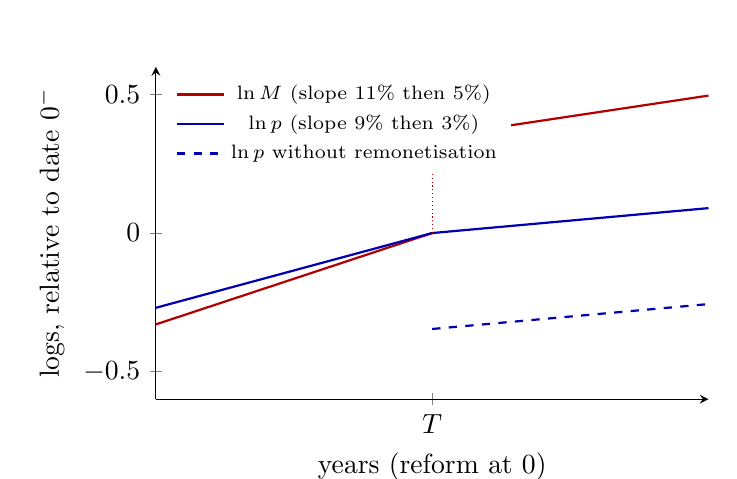
\begin{tikzpicture}
\begin{axis}[width=8.6cm,height=5.8cm,axis lines=left,xmin=-3,xmax=3,ymin=-0.6,ymax=0.6,
  xlabel={years (reform at $0$)},ylabel={logs, relative to date $0^-$},xtick={0},xticklabels={$T$},
  legend style={font=\scriptsize,draw=none,at={(0.02,0.98)},anchor=north west}]
\addplot[thick,red!70!black] coordinates {(-3,-0.33) (0,0)};
\addplot[thick,blue!70!black] coordinates {(-3,-0.27) (0,0)};
\addplot[thick,blue!70!black,dashed] coordinates {(0,-0.3466) (3,-0.2566)};
\addplot[thick,red!70!black,forget plot] coordinates {(0,0.3466) (3,0.4966)};
\addplot[thick,blue!70!black,forget plot] coordinates {(0,0) (3,0.09)};
\addplot[densely dotted,red!70!black,forget plot] coordinates {(0,0) (0,0.3466)};
\legend{$\ln M$ (slope 11\% then 5\%),$\ln p$ (slope 9\% then 3\%),$\ln p$ without remonetisation}
\end{axis}
\end{tikzpicture}\\
{\footnotesize With remonetisation $\ln M$ jumps by $\ln\sqrt2=0.35$ and $\ln p$ only changes slope. Without it,
$\ln M$ is continuous and $\ln p$ jumps down by $0.35$.}
\end{center}
\passo{5 --- the commentator}{Wrong inference. \eqref{q3b:pi} holds \emph{with $i$ constant}; at the reform $i$
falls and real money demand rises by about 41\%, so a one-time rise in $M$ of that size is exactly what keeps
prices stable. It is a \emph{level} adjustment of $M$ to a higher $m^D$, not sustained money growth. The theory
predicts both facts at once: the money stock jumps and inflation falls, because $\mu$ after the jump is low.}
\intuicao{When people expect inflation to fall, holding cash becomes cheaper and they want more of it. Either the
central bank supplies that cash, or prices fall until existing cash is worth enough.}
\refbib{Kurlat ch.~11, \S11.2, pp.~209--212, eq.~(11.2.3); \S11.1--\S11.2 on neutrality, pp.~205--215.}
\rubrica{
\item Total differentiation with $\dot i=0$ stated and $\eta$ named: 0.15. $\pi=9\%$, $i=12\%$: 0.05.
\item $\pi=3\%$, $i=6\%$, $m$ up by $\sqrt2$: 0.15. Using $\eta=1$ (quantity theory) instead of $\tfrac12$: $-0.1$.
\item Price-level jump of $-29.3\%$ or remonetisation of $41.4\%$: 0.15. Graph (slopes and the jump): 0.1.
\item Commentator: level vs growth, $m^D$ rising with lower $i$: 0.1. Agreeing with the commentator: 0 on this line.
}
\end{sol}

\parte{c}{0.6 point} Seigniorage. Compute real seigniorage per household before and after the reform, and split it
into the inflation tax and the part due to growth. Show that with the money demand of (a) seigniorage rises with
$\mu$ for every $\mu$, so there is no revenue-maximising money growth. Contrast with a Cagan semi-log demand
$M/p=Y e^{-a i}$, $a>0$: find the revenue-maximising $\mu$ and evaluate it for $a=2$. Draw both curves. Which demand
is consistent with Brazil's 1989--1993 experience, when money grew by more than 1{,}000\% a year?
\resolespaco
\begin{sol}
\begin{notacao}
\item Symbols of (a)--(b) keep their meaning. New here:
\item $S$: real seigniorage per household per year, the real value of newly issued money.
\item $a>0$: semi-elasticity of the Cagan demand $M/p=Ye^{-ai}$ with respect to $i$ ($a=2$).
\item $\mu^{\max}$: the money growth that maximises $S$ (the peak of the seigniorage Laffer curve).
\end{notacao}
\passo{1 --- definition}{Real seigniorage, multiplying and dividing by $M$:
\begin{align}
S\equiv\frac{\dot M}{p} &= \frac{\dot M}{M}\cdot\frac{M}{p}\nonumber\\
&= \mu\,m. \label{q3c:S}
\end{align}
Substitute $\mu=\pi+\eta g$ from \eqref{q3b:pi} into \eqref{q3c:S}:
\begin{align}
S &= (\pi+\eta g)\,m\nonumber\\
&= \underbrace{\pi m}_{\text{inflation tax}}+\underbrace{\eta g\,m}_{\text{growth}}. \label{q3c:split}
\end{align}}
\passo{2 --- numbers}{Before ($\mu=11\%$, $\pi=9\%$, $m=2{,}500$), by \eqref{q3c:S} and \eqref{q3c:split}:
\begin{align*}
S &= 0.11\cdot2{,}500=\boxed{275},\\
\pi m+\eta g\,m &= 0.09\cdot2{,}500+\tfrac12(0.04)\cdot2{,}500=225+50,
\end{align*}
$0.46\%$ of $Y$. After ($\mu=5\%$, $\pi=3\%$, $m=3{,}536$):
\begin{align*}
S &= 0.05\cdot3{,}536=\boxed{176.8},\\
\pi m+\eta g\,m &= 0.03\cdot3{,}536+\tfrac12(0.04)\cdot3{,}536=106.1+70.7,
\end{align*}
$0.29\%$ of $Y$. Revenue falls by 36\%, much less than $\mu$ (by 55\%), because the base rises 41\%; and the
growth part \emph{rises}: a growing economy absorbs new money without inflation.}
\passo{3 --- no peak under Baumol--Tobin}{Substitute \eqref{q3b:pi} into \eqref{q3b:fisher}:
\begin{align}
i &= r+(\mu-\eta g)\nonumber\\
&= 0.03+\mu-\tfrac12(0.04)\nonumber\\
&= \mu+0.01. \label{q3c:i}
\end{align}
Substitute \eqref{q3a:md} with \eqref{q3c:i} into \eqref{q3c:S}:
\begin{align}
S &= \mu\left(\sqrt{\frac{FY}{2i}}\right)\nonumber\\
S(\mu) &= \mu\sqrt{\frac{FY}{2(\mu+r-\eta g)}}. \label{q3c:Sbt}
\end{align}
Differentiate the log of \eqref{q3c:Sbt}, using $di/d\mu=1$ and $2i-\mu=\mu+2(r-\eta g)$:
\begin{align*}
\frac{d\ln S}{d\mu} &= \frac1\mu-\frac{1}{2i}\\
&= \frac{2i-\mu}{2\mu i}\\
&= \frac{2(\mu+r-\eta g)-\mu}{2\mu i}\\
&= \frac{\mu+2(r-\eta g)}{2\mu i}>0
\end{align*}
for all $\mu>0$, since $r-\eta g=1\%>0$. Equivalently, the elasticity of the base with respect to $\mu$ is $-\mu/(2i)>-\tfrac12>-1$: the base never shrinks
fast enough to offset the rate. \#~The Laffer peak needs a base elasticity of $-1$.}
\passo{4 --- Cagan}{The Cagan demand:
\begin{equation}
\frac Mp=Ye^{-ai}. \label{q3c:cagan}
\end{equation}
Substitute \eqref{q3c:cagan} with \eqref{q3c:i} into \eqref{q3c:S}:
\begin{align}
S &= \mu\big(Ye^{-ai}\big)\nonumber\\
&= \mu Y e^{-a(r-\eta g+\mu)}. \label{q3c:Scagan}
\end{align}
Differentiate \eqref{q3c:Scagan} with respect to $\mu$ and set it to zero:
\begin{align*}
\frac{dS}{d\mu} &= Ye^{-a(\cdot)}\,(1-a\mu)=0\\
\Rightarrow\ \mu^{\max} &= 1/a.
\end{align*}
SOC: $\frac{d^2S}{d\mu^2}=-aYe^{-a(\cdot)}(2-a\mu)<0$ at $\mu=1/a$. With $a=2$:
$\boxed{\mu^{\max}=1/a=1/2=50\%}$ a year.}
\begin{center}
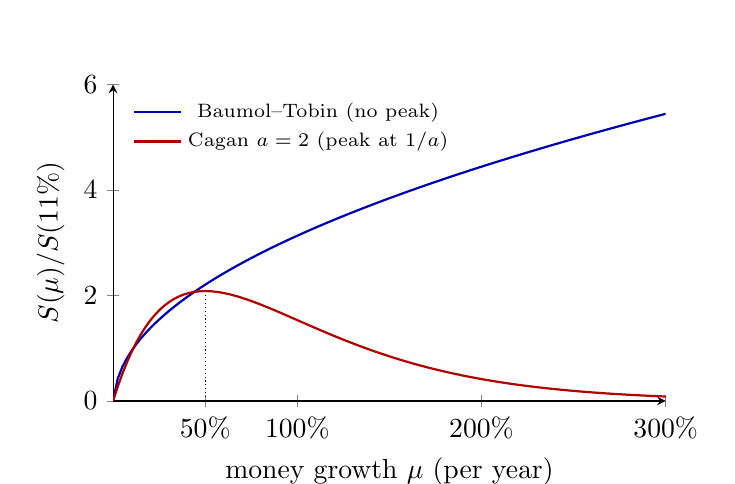
\begin{tikzpicture}
\begin{axis}[width=8.6cm,height=5.6cm,axis lines=left,xmin=0,xmax=3,ymin=0,ymax=6,
  xlabel={money growth $\mu$ (per year)},ylabel={$S(\mu)/S(11\%)$},xtick={0.5,1,2,3},
  xticklabels={50\%,100\%,200\%,300\%},
  legend style={font=\scriptsize,draw=none,at={(0.02,0.98)},anchor=north west}]
\addplot[thick,blue!70!black,domain=0:3,samples=120]{x/sqrt(x+0.01)/0.31754};
\addplot[thick,red!70!black,domain=0:3,samples=120]{x*exp(-2*(x+0.01))/0.086530};
\addplot[densely dotted] coordinates {(0.5,0) (0.5,2.0837)};
\legend{Baumol--Tobin (no peak),Cagan $a=2$ (peak at $1/a$)}
\end{axis}
\end{tikzpicture}
\end{center}
\passo{5 --- Brazil}{Rising revenue at any $\mu$, as \eqref{q3c:Sbt} implies, cannot explain why governments
printing over 1{,}000\% a year did not raise ever more revenue; with a Cagan demand \eqref{q3c:Scagan} they were
far on the \emph{wrong side} of the Laffer curve, where cutting $\mu$ costs little revenue or even raises it.
Baumol--Tobin with a fixed $F$ misses the flight from money at high inflation (indexed overnight accounts lowered
the effective $F$ and made demand far more elastic).}
\intuicao{Seigniorage is a tax with rate $\mu$ on the base $M/p$. Whether raising the rate raises revenue depends on
how fast the base flees; under Baumol--Tobin it flees too slowly to ever turn revenue down.}
\refbib{Kurlat ch.~11, \S11.3, pp.~215--216 (seigniorage); the Cagan demand is used in ex.~11.6, p.~218, which
works the limit on revenue with another functional form.}
\rubrica{
\item $S=\mu m$ and the split: 0.1. Both numbers and splits: 0.15 (slip: $-0.1$).
\item Proof of no peak (derivative signed, or elasticity $>-1$): 0.15. Asserting it without proof: 0 on this line.
\item Cagan peak with SOC and 50\%: 0.1. Graph (both curves, peak marked): 0.05.
\item Brazil reading: 0.05.
}
\end{sol}

\parte{d}{0.6 point} Costs of inflation. Compute the real resources spent on trips to the bank, in reais and as a
share of $Y$, before and after the reform. Why is the forgone interest on cash not counted as a cost to society?
Find the inflation and money-growth rates of the Friedman rule, and say what happens to the Baumol--Tobin solution
there. Give two reasons why the central bank targets 3\% rather than this rate.
\resolespaco
\begin{sol}
\begin{notacao}
\item Symbols of (a)--(c) keep their meaning. New here:
\item $R\ge0$: real resources spent on trips to the bank per year (shoe-leather cost), $R=FN^*$.
\item Friedman rule: the policy that sets the nominal interest rate to zero, $i=0$.
\end{notacao}
\passo{1 --- trips}{The resource cost is the number of trips times their real cost. Substitute
\eqref{q3a:N}:
\begin{align}
R=FN^* &= F\left(\sqrt{\frac{iY}{2F}}\right)\nonumber\\
&= \boxed{\sqrt{\frac{iFY}{2}}}. \label{q3d:R}
\end{align}
Before ($i=12\%$, $N^*=12$) and after ($i=6\%$), by \eqref{q3d:R}:
\begin{align*}
R_{\text{before}} &= 25\cdot12=\boxed{300},\quad 0.50\%\ \text{of }Y,\\
R_{\text{after}} &= \sqrt{\frac{0.06\cdot25\cdot60{,}000}{2}}=\sqrt{45{,}000}=\boxed{212.1},\quad 0.35\%\ \text{of }Y.
\end{align*}
The reform saves $0.15\%$ of income every year (shoe-leather cost).}
\passo{2 --- forgone interest}{Multiply \eqref{q3a:md} by $i$: at the optimum the forgone interest is
\[
i\,\frac Mp=i\left(\sqrt{\frac{FY}{2i}}\right)=\sqrt{\frac{iFY}{2}},
\]
the same as \eqref{q3d:R} (300 before), but it is not a use of resources: the inflation-tax part
($\pi m=225$, \eqref{q3c:split}) is revenue of the government, and the rest is a transfer to whoever borrows the
funds. Only the trips burn goods. (Total private cost $\sqrt{2iFY}=600$.)}
\passo{3 --- Friedman rule}{Set $i=0$ in \eqref{q3b:fisher}, then use \eqref{q3b:pi} solved for $\mu$:
\begin{align*}
(0) &= r+\pi\\
\pi &= -r=\boxed{-3\%},\\
\mu &= \pi+\eta g=(-3\%)+\tfrac12(4\%)=\boxed{-1\%}.
\end{align*}
Then, by \eqref{q3a:N} and \eqref{q3a:md}, $N^*\to0$ and $M/p\to\infty$. The interior solution needs $N^*\ge1$;
by \eqref{q3a:N}:
\[
\frac{iY}{2F}\ge1\iff i\ge\frac{2F}{Y}=\frac{2\cdot25}{60{,}000}=0.083\%;
\]
below that the household makes one trip and holds $Y/2=30{,}000$. Shoe-leather costs vanish.}
\passo{4 --- why 3\%}{(i) Measured inflation overstates true inflation (substitution, quality and new-goods biases
of a Laspeyres index), so 0 measured is deflation. (ii) With $\pi=-3\%$, $i$ would sit at zero in normal times,
leaving no room to cut it in a recession --- the zero lower bound of Question 4. (iii) Nominal wages are rigid
downward; some inflation lets real wages fall.}
\intuicao{Inflation is a tax on holding cash; people spend real resources dodging it. The Friedman rule removes the
tax, but a central bank that needs room to cut rates gives up a little of that gain.}
\refbib{Kurlat ch.~11, \S11.4, pp.~216--222 (costs of inflation, Friedman rule); ch.~10, \S10.4.}
\rubrica{
\item Trip cost formula and both numbers with shares: 0.2 (slip: $-0.1$). Counting $i\,m$ as the social cost: max.\ 0.1 on this line.
\item Transfer argument: 0.1. Friedman rule $\pi=-3\%$, $\mu=-1\%$: 0.1; the corner $N\ge1$: 0.05.
\item Two valid reasons for a positive target: 0.15.
}
\gap{Kurlat ch.~10--11 were absent from Prova 01: Baumol--Tobin from primitives, $\pi=\mu-\eta g$ by total
differentiation, Fisher, seigniorage and its Laffer curve.}
\end{sol}

% =============================================================================
\questao{(3.0 points) The Copom between a tax shock and a liquidity trap.
Use Benigno (2015), in log deviations from an efficient steady state, with a short run and a long run:
\begin{align}
y &= \bar y_n+(g-\bar g)-\sigma\left[i-(\bar p-p)-\rho\right], \tag{AD}\label{q4:AD}\\
p-p^e &= \kappa(y-y_n), \tag{AS}\label{q4:AS}\\
y_n &= \frac{(1+\eta)a+\sigma^{-1}g-\mu}{\sigma^{-1}+\eta}, \tag{YN}\label{q4:YN}\\
y_e &= \frac{(1+\eta)a+\sigma^{-1}g}{\sigma^{-1}+\eta}. \tag{YE}\label{q4:YE}
\end{align}
Initially $a=g=\bar g=\mu=0$, $\bar y_n=0$, $\bar p=p^e=0$ and $i=\rho$. Take $\sigma=1$, $\eta=1$, $\kappa=1/2$ and
$\rho=2\%$; $y$ and $p$ are in percent. The Copom sets $i$ to minimise
\begin{equation}
L=\tfrac12(y-y_e)^2+\frac{\phi}{2\kappa}(p-p^e)^2,\qquad \phi>0. \tag{LF}\label{q4:LF}
\end{equation}}

\parte{a}{0.8 point} A temporary rise in a federal tax on firms' revenues raises the mark-up by $\mu=4$ in the
current period only. Find the changes in $y_n$ and $y_e$ and say which curve shifts. Derive the Copom's optimal
targeting rule by substituting the relevant constraint into the loss, and the optimal $y$ and $p$ as functions of
$\phi$; evaluate them for $\phi=4$. Explain why the Copom cannot reach $y=y_e$ and $p=p^e$ together here, while it
could after a temporary productivity shock. Show graphically.
\resolespaco
\begin{sol}
\begin{notacao}
\item $y$, $p$: output and price level today, log deviations from the steady state, in percent.
\item $\bar y_n$, $\bar p$: long-run natural output and long-run price level. $p^e$: the price preset by firms
that cannot adjust this period.
\item $i\ge0$: nominal policy rate, the Copom's instrument. $\rho>0$: rate of time preference, the steady-state
real rate ($\rho=2\%$).
\item $g$, $\bar g$: government spending today and in the long run. $a$: productivity. $\mu$: firms' mark-up
(here raised by the tax).
\item $\sigma>0$: intertemporal elasticity of substitution (not the capital share of Q1). $\eta>0$: inverse
Frisch elasticity of labour supply. $\kappa>0$: slope of AS.
\item $y_n$: natural output (flexible prices, with the mark-up). $y_e$: efficient output (no mark-up).
\item $\phi>0$: weight on price surprises in the loss $L$ \eqref{q4:LF}.
\item $\Delta\equiv y_e-y_n$: the gap between efficient and natural output (defined in Step 1).
\item $y^*$, $p^*$: the optimal point. $E_0$: initial equilibrium. $E'$: the outcome with $i=\rho$. $O$: the optimum.
\end{notacao}
\passo{1 --- what moves}{Differentiate \eqref{q4:YN} and \eqref{q4:YE} with respect to $\mu$:
\begin{align}
dy_n &= -\frac{\mu}{\sigma^{-1}+\eta}=-\frac{4}{1+1}=\boxed{-2}, \label{q4a:dyn}\\
dy_e &= \boxed{0}\qquad(\mu\text{ is not in }y_e). \label{q4a:dye}
\end{align}
\textbf{AS shifts up/left}: by \eqref{q4:AS} it now passes through $(y_n',p^e)=(-2,0)$, so at each $y$ the price
is higher by $\kappa\cdot2=1$. \textbf{AD does not move}: $\mu$ is not in \eqref{q4:AD} and, the shock being
temporary, $\bar y_n$ is unchanged. From \eqref{q4a:dyn}--\eqref{q4a:dye}:
\begin{equation}
\Delta\equiv y_e-y_n=0-(-2)=2>0. \label{q4a:Delta}
\end{equation}}
\passo{2 --- the constraint}{The Copom moves AD with $i$, so it can pick \emph{any} point on AS; AS ($p^e$ is
predetermined) is the constraint. Substitute \eqref{q4:AS} into \eqref{q4:LF}:
\begin{align}
L(y) &= \tfrac12(y-y_e)^2+\frac{\phi}{2\kappa}\big(\kappa(y-y_n)\big)^2\nonumber\\
&= \tfrac12(y-y_e)^2+\frac{\phi}{2\kappa}\kappa^2(y-y_n)^2\nonumber\\
&= \tfrac12(y-y_e)^2+\frac{\phi\kappa}{2}(y-y_n)^2. \label{q4a:Ly}
\end{align}}
\passo{3 --- targeting rule}{Differentiate \eqref{q4a:Ly} and set it to zero (SOC $1+\phi\kappa>0$):
\begin{equation}
\frac{dL}{dy}=(y-y_e)+\phi\kappa(y-y_n)=0. \label{q4a:foc}
\end{equation}
By \eqref{q4:AS}, $\kappa(y-y_n)=p-p^e$. Substitute this into \eqref{q4a:foc}:
\begin{equation}
\boxed{(y-y_e)+\phi\,(p-p^e)=0}. \label{q4a:rule}
\end{equation}
Solve \eqref{q4a:foc} for $y$, then use $y_e=0$ and $y_n=-\Delta$ from \eqref{q4a:Delta}:
\begin{align}
y(1+\phi\kappa) &= y_e+\phi\kappa\,y_n\nonumber\\
y^* &= \frac{y_e+\phi\kappa\,y_n}{1+\phi\kappa}\nonumber\\
&= \frac{(0)+\phi\kappa\,(-\Delta)}{1+\phi\kappa}\nonumber\\
&= -\frac{\phi\kappa\,\Delta}{1+\phi\kappa}. \label{q4a:ystar}
\end{align}
Subtract $y_n=-\Delta$ from \eqref{q4a:ystar} and substitute into \eqref{q4:AS}:
\begin{align}
y^*-y_n &= \left(-\frac{\phi\kappa\,\Delta}{1+\phi\kappa}\right)-(-\Delta)\nonumber\\
&= \frac{\Delta}{1+\phi\kappa},\nonumber\\
p^*-p^e &= \kappa(y^*-y_n)\nonumber\\
&= \kappa\left(\frac{\Delta}{1+\phi\kappa}\right)\nonumber\\
&= \frac{\kappa\,\Delta}{1+\phi\kappa}. \label{q4a:pstar}
\end{align}
With $\phi=4$, $\phi\kappa=2$; by \eqref{q4a:ystar} and \eqref{q4a:pstar}:
\begin{align*}
y^* &= -\frac{2\cdot2}{1+2}=\boxed{-1.33\%},\\
p^* &= \frac{0.5\cdot2}{1+2}=\boxed{+0.33\%}.
\end{align*}
Check in \eqref{q4a:rule}: $-\tfrac43+4\cdot\tfrac13=0$ \checkmark.}
\passo{4 --- divine coincidence fails}{Both targets require $y=y_e=0$ and $p=p^e$, but on the new AS
\eqref{q4:AS}, $p-p^e=\kappa(0+2)=1\neq0$ at $y=0$: the bliss point is not on the constraint, and one instrument
cannot hit two targets. After a temporary productivity shock, \eqref{q4:YN} and \eqref{q4:YE} move $y_n$ and $y_e$
by the same $\frac{1+\eta}{\sigma^{-1}+\eta}a$, so $(y_e,p^e)$ lies on the new AS and the Copom puts AD through it:
zero loss, whatever $\phi$.}
\begin{center}
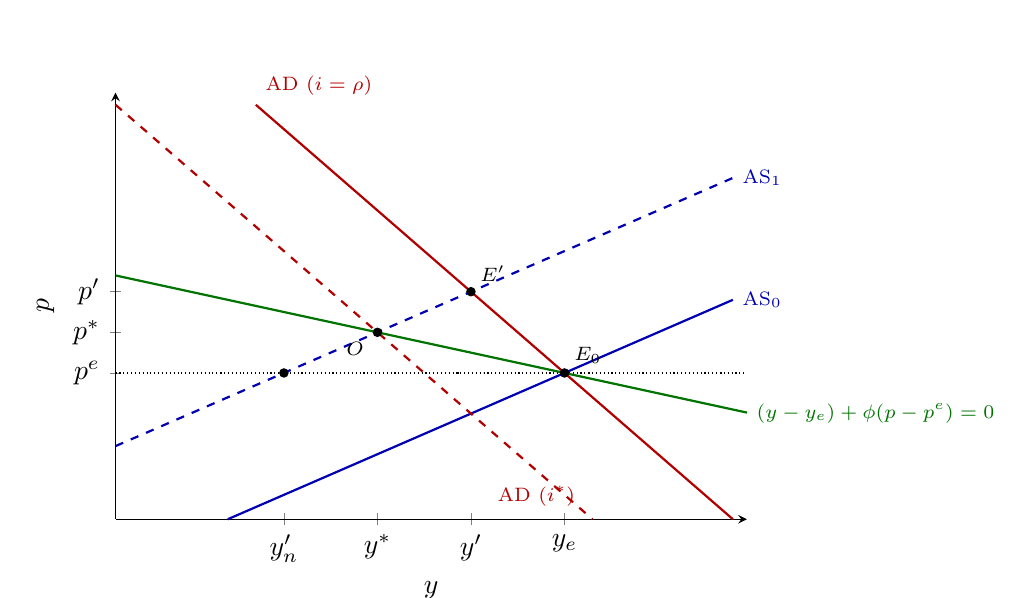
\begin{tikzpicture}
\begin{axis}[width=9.6cm,height=7cm,axis lines=left,xmin=-3.2,xmax=1.3,ymin=-1.2,ymax=2.3,clip=false,
  xlabel={$y$},ylabel={$p$},
  xtick={-2,-1.3333,-0.6667,0},xticklabels={$y_n'$,$y^*$,$y'$,$y_e$},ytick={0,0.3333,0.6667},
  yticklabels={$p^e$,$p^*$,$p'$}]
\addplot[densely dotted,domain=-3.2:1.3]{0};
\addplot[thick,blue!70!black,domain=-2.4:1.2]{0.5*x};
\addplot[thick,blue!70!black,dashed,domain=-3.2:1.2]{0.5*(x+2)};
\addplot[thick,red!70!black,domain=-2.2:1.2]{-x};
\addplot[thick,red!70!black,dashed,domain=-3.2:0.2]{-x-1};
\addplot[thick,green!45!black,domain=-3.2:1.3]{-x/4};
\addplot[only marks,mark=*,mark size=1.5pt] coordinates {(0,0) (-0.6667,0.6667) (-1.3333,0.3333) (-2,0)};
\node[font=\scriptsize,blue!70!black,anchor=west] at (axis cs:1.2,0.6) {AS$_0$};
\node[font=\scriptsize,blue!70!black,anchor=west] at (axis cs:1.2,1.6) {AS$_1$};
\node[font=\scriptsize,red!70!black,anchor=south west] at (axis cs:-2.2,2.2) {AD ($i=\rho$)};
\node[font=\scriptsize,red!70!black,anchor=north] at (axis cs:-0.2,-0.85) {AD ($i^*$)};
\node[font=\scriptsize,green!45!black,anchor=west] at (axis cs:1.3,-0.33) {$(y-y_e)+\phi(p-p^e)=0$};
\node[font=\scriptsize,anchor=south west] at (axis cs:-0.67,0.67) {$E'$};
\node[font=\scriptsize,anchor=north east] at (axis cs:-1.36,0.33) {$O$};
\node[font=\scriptsize,anchor=south west] at (axis cs:0,0) {$E_0$};
\end{axis}
\end{tikzpicture}\\
{\footnotesize AS shifts up through $(y_n',p^e)$; with $i=\rho$ the economy goes to $E'=(-0.67,\,0.67)$ along the
unmoved AD. The optimum $O=(-1.33,\,0.33)$ is where AS$_1$ meets the targeting line (slope $-1/\phi$, through
the bliss point $E_0$); the Copom raises $i$ to move AD down to $O$.}
\end{center}
\intuicao{A mark-up shock makes the economy's natural output inefficiently low. Pushing output up to the efficient
level costs inflation; holding prices costs output. With convex losses the Copom splits the difference, and $\phi$
says how much it dislikes the price side.}
\refbib{Benigno (2015), \S7 (mark-up shocks), Fig.~9, pp.~513--514; \S11, eqs.~(33)--(35), Fig.~14, pp.~521--523;
\S4.2--\S4.4 for $y_n$ vs $y_e$, pp.~508--509.}
\rubrica{
\item $dy_n=-2$, $dy_e=0$, AS shifts and AD does not, with reasons: 0.2. Shifting AD: max.\ 0.3 on the item.
\item Substituting AS into the loss and $dL/dy=0$; the targeting rule: 0.2. Minimising along AD or treating $i$ as
the choice with AD as the constraint: max.\ 0.3 on the item.
\item $y^*$, $p^*$ in general and $-1.33$, $+0.33$: 0.15 (slip: $-0.1$).
\item Divine-coincidence argument and the productivity contrast: 0.1.
\item Graph: axes, AS$_0$/AS$_1$, AD, the targeting line, $E'$ and $O$: 0.15.
}
\end{sol}

\parte{b}{0.6 point} Find the policy rate $i^*$ that implements the optimum, for general $\phi$ and for $\phi=4$, and
compare it with keeping $i=\rho$. Show that the Copom raises the rate if and only if $\phi>\sigma$. Interpret
$\phi\to0$, $\phi\to\infty$ and the knife edge $\phi=\sigma$, using the graph of (a).
\resolespaco
\begin{sol}
\begin{notacao}
\item Symbols of (a) keep their meaning. New here:
\item $i^*$: the policy rate that implements $(y^*,p^*)$.
\item $y'$, $p'$: the outcome if the Copom keeps $i=\rho$ (point $E'$).
\end{notacao}
\passo{1 --- invert AD}{Set $\bar y_n=g=\bar g=\bar p=0$ in \eqref{q4:AD}:
\begin{align}
y &= (0)+(0-0)-\sigma\big[i-(0-p)-\rho\big]\nonumber\\
&= -\sigma(i-\rho)-\sigma p. \label{q4b:ad}
\end{align}
Solve \eqref{q4b:ad} for the rate:
\begin{equation}
i-\rho=-\frac{y+\sigma p}{\sigma}. \label{q4b:inv}
\end{equation}}
\passo{2 --- the rate}{Add \eqref{q4a:ystar} and $\sigma$ times \eqref{q4a:pstar} (with $p^e=0$):
\begin{align*}
y^*+\sigma p^* &= \left(-\frac{\phi\kappa\Delta}{1+\phi\kappa}\right)+\sigma\left(\frac{\kappa\Delta}{1+\phi\kappa}\right)\\
&= \frac{-\phi\kappa\Delta+\sigma\kappa\Delta}{1+\phi\kappa}\\
&= -\frac{\kappa(\phi-\sigma)\Delta}{1+\phi\kappa}.
\end{align*}
Substitute into \eqref{q4b:inv}:
\begin{align}
i^*-\rho &= -\frac{1}{\sigma}\left(-\frac{\kappa(\phi-\sigma)\Delta}{1+\phi\kappa}\right)\nonumber\\
&= \boxed{\frac{\kappa(\phi-\sigma)\,\Delta}{\sigma(1+\phi\kappa)}}. \label{q4b:istar}
\end{align}
With $\phi=4$:
\[
i^*-\rho=\frac{0.5\cdot(4-1)\cdot2}{1\cdot(1+2)}=1\ \Rightarrow\ \boxed{i^*=3\%}.
\]
Check on \eqref{q4b:ad}: $-1\cdot(3-2)-1\cdot\tfrac13=-\tfrac43=y^*$ \checkmark. With $i=\rho$, \eqref{q4b:ad} gives
$y=-\sigma p$; substitute \eqref{q4:AS}, $p=\kappa(y-y_n')$:
\begin{align*}
y &= -\sigma\big(\kappa(y-y_n')\big)\\
y(1+\sigma\kappa) &= \sigma\kappa\,y_n'\\
y' &= \frac{\sigma\kappa}{1+\sigma\kappa}y_n'=\frac{0.5}{1.5}(-2)=-0.67,\\
p' &= -y'/\sigma=-(-0.67)/1=+0.67.
\end{align*}
Loss \eqref{q4:LF} ($\phi/2\kappa=4$) at $E'$ and at the optimum $O$:
\begin{align*}
L(E') &= \tfrac12\big(\tfrac23\big)^2+4\big(\tfrac23\big)^2=\tfrac29+\tfrac{16}9=2.0,\\
L(O) &= \tfrac12\big(\tfrac43\big)^2+4\big(\tfrac13\big)^2=\tfrac89+\tfrac49=1.33.
\end{align*}}
\passo{3 --- sign}{In \eqref{q4b:istar}, $\kappa,\Delta,\sigma,1+\phi\kappa>0$, so
\[
\operatorname{sign}(i^*-\rho)=\operatorname{sign}(\phi-\sigma):\quad\boxed{\text{raise iff }\phi>\sigma}.
\]
Doing nothing leaves, from the lines above, $y'-y_n'=\frac{\Delta}{1+\sigma\kappa}$; the optimum
\eqref{q4a:pstar} wants $y^*-y_n=\frac{\Delta}{1+\phi\kappa}$, smaller iff $\phi>\sigma$, which needs a lower AD,
i.e.\ a higher rate.}
\passo{4 --- limits}{Take limits in \eqref{q4b:istar}, \eqref{q4a:ystar} and \eqref{q4a:pstar}:
\begin{itemize}[leftmargin=1.4em]
\item $\phi\to0$: $i^*-\rho\to-\kappa\Delta=-1$, $i^*=1\%$: the Copom \emph{cuts}, sets $y=y_e=0$ and accepts
$p=+1\%$.
\item $\phi\to\infty$: $i^*-\rho\to\Delta/\sigma=2$, $i^*=4\%$: strict price stability, $p=p^e$, $y=y_n'=-2$.
\item $\phi=\sigma$: $i^*=\rho$.
\end{itemize}
Geometrically the targeting line \eqref{q4a:rule} (slope $-1/\phi$) and AD \eqref{q4b:ad} (slope $-1/\sigma$)
both pass through the bliss point $E_0$; when $\phi=\sigma$ they coincide, so AD at $i=\rho$ already meets AS$_1$
on the targeting line.}
\intuicao{Doing nothing already splits the shock between prices and output in a proportion set by $\sigma$ (how
strongly demand reacts to the real rate). The Copom tightens only if it cares about prices more than that
built-in split does.}
\refbib{Benigno (2015), \S11, pp.~521--523; \S5, eqs.~(20)--(21), pp.~509--511.}
\rubrica{
\item AD inverted and $i^*$ in general: 0.2; $i^*=3\%$ with the comparison to $i=\rho$: 0.1.
\item Sign proof ($\phi>\sigma$): 0.15. Stating the sign without proof: 0 on this line. Saying the response does not
depend on $\phi$ (true only for AD shocks): max.\ 0.2 on the item.
\item The three cases, each with its reading: 0.15.
}
\end{sol}

\parte{c}{0.7 point} Two years later the tax is gone ($\mu=0$), but a household-debt crisis makes households expect
lower long-run income: $\bar y_n$ falls by 4\%, with $y_n$ and $y_e$ unchanged. Find the natural real rate $r_n$ and
the rate the Copom would like to set. Given $i\ge0$, find $y$, $p$ and the gaps when $i=0$, and show the outcome
graphically. What promise about $\bar p$ would take the economy to $(y_e,p^e)$ with $i=0$, and what does it require?
\resolespaco
\begin{sol}
\begin{notacao}
\item Symbols of (a)--(b) keep their meaning; now $\mu=0$, so $y_n=y_e=0$. New here:
\item $\bar y_n=-4$: long-run natural output after the household-debt crisis.
\item $r_n$: the natural real rate, the $i$ that delivers $y=y_n$ with $p=p^e=\bar p$.
\item $i\ge0$: the zero lower bound (ZLB). $Z$: the outcome at $i=0$.
\end{notacao}
\passo{1 --- natural rate}{Put $y=y_n$, $p=p^e=\bar p$ (so $\bar p-p=0$), $g=\bar g=0$ and $i=r_n$ in
\eqref{q4:AD}:
\begin{align*}
y_n &= \bar y_n+(0-0)-\sigma\big[r_n-(0)-\rho\big]\\
&= \bar y_n-\sigma(r_n-\rho).
\end{align*}
Solve for $r_n$:
\begin{equation}
\boxed{r_n=\rho+\sigma^{-1}(\bar y_n-y_n)}. \label{q4c:rn}
\end{equation}
Numbers in \eqref{q4c:rn}: $r_n=2+1^{-1}(-4-0)=\boxed{-2\%}$. This is a pure AD shock (AS does not move), so the divine
coincidence holds and the Copom wants $i=r_n=-2\%$.}
\passo{2 --- the ZLB binds}{$i=-2\%$ is infeasible; the best it can do is $i=0$. Put $i=0$, $\bar y_n=-4$,
$\bar p=0$ in \eqref{q4:AD}:
\begin{align}
y &= (-4)+(0-0)-1\cdot\big[(0)-(0-p)-2\big]\nonumber\\
&= -2-p. \label{q4c:ad}
\end{align}
AS \eqref{q4:AS} with $p^e=0$, $y_n=0$, $\kappa=\tfrac12$:
\begin{align}
p-(0) &= \tfrac12\big(y-(0)\big)\nonumber\\
p &= \tfrac12y. \label{q4c:as}
\end{align}
Substitute \eqref{q4c:as} into \eqref{q4c:ad}:
\begin{align*}
y &= -2-\left(\tfrac12y\right)\\
\tfrac32y &= -2\\
y &= \boxed{-1.33\%}.
\end{align*}
Back into \eqref{q4c:as}: $p=\tfrac12(-\tfrac43)=\boxed{-0.67\%}$. Gaps: $y-y_n=y-y_e=\boxed{-1.33}$; prices fall.
Loss \eqref{q4:LF} with $\phi=4$:
\begin{align*}
L &= \tfrac12\left(-\tfrac43\right)^2+4\left(-\tfrac23\right)^2\\
&= \tfrac12(1.78)+4(0.44)=2.67.
\end{align*}}
\passo{3 --- forward guidance}{Keep $i=0$ but let $\bar p$ be free in \eqref{q4:AD}:
\begin{equation}
y=-4-\big[0-\bar p+p-2\big]. \label{q4c:fg}
\end{equation}
Require $(y,p)=(0,0)$ in \eqref{q4c:fg}:
\begin{align*}
(0) &= -4-\big[0-\bar p+(0)-2\big]\\
0 &= -4+\bar p+2\\
\bar p &= \boxed{+2\%=-r_n}.
\end{align*}
A higher future price level is expected inflation $\bar p-p=2$, which takes the real rate $i-(\bar p-p)$ to
$-2\%=r_n$ with $i=0$. It requires \textbf{credibility}: the Copom must convince people it will tolerate a higher
price level later, when it would be tempted to renege.}
\begin{center}
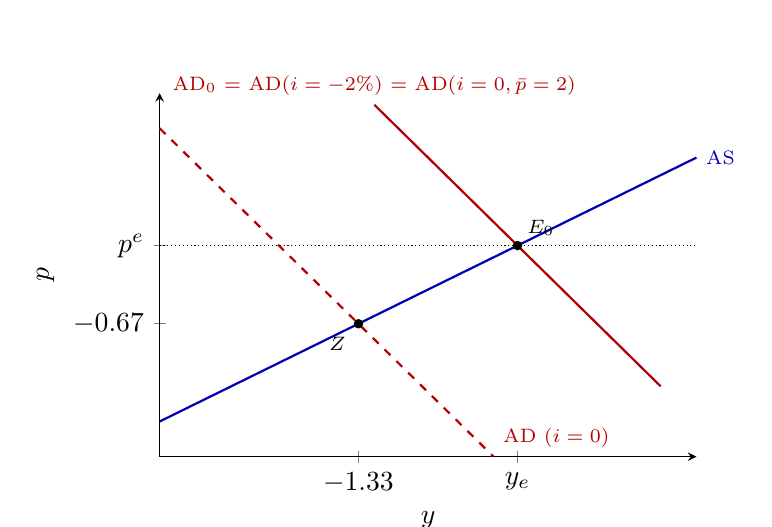
\begin{tikzpicture}
\begin{axis}[width=8.4cm,height=6.2cm,axis lines=left,xmin=-3,xmax=1.5,ymin=-1.8,ymax=1.3,clip=false,
  xlabel={$y$},ylabel={$p$},
  xtick={-1.3333,0},xticklabels={$-1.33$,$y_e$},ytick={-0.6667,0},yticklabels={$-0.67$,$p^e$}]
\addplot[densely dotted,domain=-3:1.5]{0};
\addplot[thick,blue!70!black,domain=-3:1.5]{0.5*x};
\addplot[thick,red!70!black,domain=-1.2:1.2]{-x};
\addplot[thick,red!70!black,dashed,domain=-3:-0.2]{-2-x};
\addplot[only marks,mark=*,mark size=1.5pt] coordinates {(0,0) (-1.3333,-0.6667)};
\node[font=\scriptsize,blue!70!black,anchor=west] at (axis cs:1.5,0.75) {AS};
\node[font=\scriptsize,red!70!black,anchor=south] at (axis cs:-1.2,1.2) {AD$_0$ $=$ AD($i=-2\%$) $=$ AD($i=0,\bar p=2$)};
\node[font=\scriptsize,red!70!black,anchor=south west] at (axis cs:-0.2,-1.8) {AD ($i=0$)};
\node[font=\scriptsize,anchor=north east] at (axis cs:-1.36,-0.70) {$Z$};
\node[font=\scriptsize,anchor=south west] at (axis cs:0,0) {$E_0$};
\end{axis}
\end{tikzpicture}\\
{\footnotesize The fall in $\bar y_n$ shifts AD left by 4; at $i=0$ it can only be brought back by 2, so the economy
sits at $Z$. Either $i=-2\%$ (infeasible) or $\bar p=2\%$ (a promise) puts AD back through $E_0$.}
\end{center}
\intuicao{Expecting to be poorer later, households cut consumption now. Only a negative real rate would persuade
them to spend; with $i$ stuck at zero, that negative real rate has to come from expected inflation.}
\refbib{Benigno (2015), \S9 (liquidity trap), Figs.~11--12, pp.~516--518; natural rate from \S5.}
\rubrica{
\item $r_n=-2\%$ derived and the desired $i$: 0.15. Calling it a supply shock or a trade-off: max.\ 0.2 on the item.
\item ZLB equilibrium $y=-1.33$, $p=-0.67$, gaps: 0.2 (slip: $-0.1$).
\item $\bar p=2\%$ and the real-rate mechanism, credibility: 0.2.
\item Graph: AS, AD shifted left, the partial return at $i=0$, point $Z$: 0.15.
}
\end{sol}

\parte{d}{0.9 point} Instead of a promise, the government raises current spending $g$ ($\bar g$ unchanged) while
$i$ stays at 0. Derive the multipliers $dy/dg$ and $d(y-y_e)/dg$, evaluate them, find the $g$ that closes the gap,
and check what happens to $p$. Then suppose the Copom were away from the ZLB and followed its optimal rule: what
would $dy/dg$ be? Explain why the ZLB makes fiscal policy more powerful here. Does Benigno's \S10 suggest even larger
multipliers? Show the effect of $g$ on the graph.
\resolespaco
\begin{sol}
\begin{notacao}
\item Symbols of (a)--(c) keep their meaning. New here:
\item $g\ge0$: current government spending, in percent of GDP; $\bar g=0$ unchanged.
\item $\omega\equiv\dfrac{\sigma^{-1}}{\sigma^{-1}+\eta}\in(0,1)$: response of $y_n$ and $y_e$ to $g$.
\item $dy/dg$: output multiplier. $d(y-y_e)/dg$: gap multiplier. $F$: the outcome with $g=4$.
\end{notacao}
\passo{1 --- $g$ moves both curves}{AD \eqref{q4:AD}: $+g$ one-for-one. AS: differentiate \eqref{q4:YN} and
\eqref{q4:YE} with respect to $g$:
\begin{equation}
\frac{dy_n}{dg}=\frac{dy_e}{dg}=\omega=\tfrac12, \label{q4d:omega}
\end{equation}
the wealth effect of taxes-to-come on labour supply. $y_n$ and $y_e$ rise by the same $\omega g$, so $g$ is not a
mark-up shock.}
\passo{2 --- solve}{Put $i=0$, $\bar p=0$, $\bar g=0$ in \eqref{q4:AD}:
\begin{align}
y &= \bar y_n+(g-0)-\sigma\big[(0)-(0-p)-\rho\big]\nonumber\\
&= \bar y_n+\sigma\rho+g-\sigma p. \label{q4d:ad}
\end{align}
AS \eqref{q4:AS} with $p^e=0$ and $y_n=\omega g$ from \eqref{q4d:omega}:
\begin{align}
p-(0) &= \kappa\big(y-(\omega g)\big)\nonumber\\
p &= \kappa(y-\omega g). \label{q4d:as}
\end{align}
Substitute \eqref{q4d:as} into \eqref{q4d:ad}:
\begin{align*}
y &= \bar y_n+\sigma\rho+g-\sigma\big(\kappa(y-\omega g)\big)\\
&= \bar y_n+\sigma\rho+g-\sigma\kappa y+\sigma\kappa\omega g\\
y(1+\sigma\kappa) &= \bar y_n+\sigma\rho+g(1+\sigma\kappa\omega).
\end{align*}
Differentiate with respect to $g$:
\begin{equation}
\boxed{\frac{dy}{dg}=\frac{1+\sigma\kappa\,\omega}{1+\sigma\kappa}}
=\frac{1+1\cdot\frac12\cdot\frac12}{1+1\cdot\frac12}=\boxed{\tfrac56}.
\label{q4d:mult}
\end{equation}
Subtract \eqref{q4d:omega} from \eqref{q4d:mult}:
\begin{align}
\frac{d(y-y_e)}{dg} &= \frac{1+\sigma\kappa\omega}{1+\sigma\kappa}-\omega\nonumber\\
&= \frac{1+\sigma\kappa\omega-\omega-\sigma\kappa\omega}{1+\sigma\kappa}\nonumber\\
&= \boxed{\frac{1-\omega}{1+\sigma\kappa}}=\frac{1-\frac12}{1+1\cdot\frac12}=\boxed{\tfrac13}. \label{q4d:gap}
\end{align}
These are Benigno's Table~1 $m_g=\frac{1}{1+\sigma\kappa}+\frac{\kappa}{(\sigma^{-1}+\eta)(1+\sigma\kappa)}$ and
$m_{\bar g}=\frac{\eta}{(\sigma^{-1}+\eta)(1+\sigma\kappa)}$ (with $\sigma\kappa\omega=\kappa/(\sigma^{-1}+\eta)$ and
$1-\omega=\eta/(\sigma^{-1}+\eta)$).}
\passo{3 --- closing the gap}{The gap at $Z$ is $-\tfrac43$ (part (c)). Divide by \eqref{q4d:gap}:
\[
g=\frac{4/3}{1/3}=\boxed{4\%}\ \text{of GDP}.
\]
Then, by \eqref{q4d:mult}, \eqref{q4d:omega} and \eqref{q4d:as}:
\begin{align*}
y &= -\tfrac43+\tfrac56\cdot4=\boxed{2},\\
y_n &= y_e=\omega g=\tfrac12\cdot4=2,\\
p &= \kappa(y-y_n)=\tfrac12(2-2)=\boxed{0=p^e}:
\end{align*}
both gaps closed, zero loss.}
\passo{4 --- away from the ZLB}{By \eqref{q4d:omega} spending moves $y_n$ and $y_e$ together, so there is no
trade-off: the optimal Copom satisfies \eqref{q4a:rule} with both gaps zero, $y=y_e(g)=\omega g$, $p=p^e$, raising
$i$ by $(1-\omega)g/\sigma$ to offset the excess demand in \eqref{q4:AD}. Then
$\boxed{dy/dg=\omega=\tfrac12}$.}
\passo{5 --- why larger at the ZLB}{Compare \eqref{q4d:mult} with $\omega$:
\[
\frac{1+\sigma\kappa\omega}{1+\sigma\kappa}>\omega\iff1>\omega\iff\eta>0.
\]
At the ZLB the Copom does not raise $i$ (it would like a \emph{lower} rate), so there is no crowding out through
the policy rate; only the price channel (a higher $p$ with $\bar p$ given raises the real rate) remains, which
keeps the multiplier below 1. In \S10 (Eggertsson--Krugman deleveraging) some households are
borrowing-constrained and spend every extra real of income, and falling prices raise real debt burdens: there the
multiplier at the ZLB can be much larger. With one representative household, as here, it stays at $5/6$.}
\begin{center}
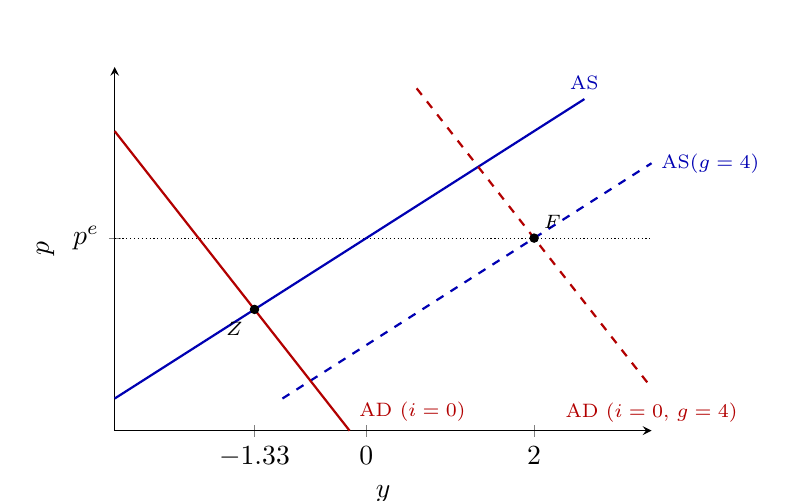
\begin{tikzpicture}
\begin{axis}[width=8.4cm,height=6.2cm,axis lines=left,xmin=-3,xmax=3.4,ymin=-1.8,ymax=1.6,clip=false,
  xlabel={$y$},ylabel={$p$},
  xtick={-1.3333,0,2},xticklabels={$-1.33$,$0$,$2$},ytick={0},yticklabels={$p^e$}]
\addplot[densely dotted,domain=-3:3.4]{0};
\addplot[thick,blue!70!black,domain=-3:2.6]{0.5*x};
\addplot[thick,blue!70!black,dashed,domain=-1:3.4]{0.5*(x-2)};
\addplot[thick,red!70!black,domain=-3:-0.2]{-2-x};
\addplot[thick,red!70!black,dashed,domain=0.6:3.4]{2-x};
\addplot[only marks,mark=*,mark size=1.5pt] coordinates {(-1.3333,-0.6667) (2,0)};
\node[font=\scriptsize,blue!70!black,anchor=south] at (axis cs:2.6,1.3) {AS};
\node[font=\scriptsize,blue!70!black,anchor=west] at (axis cs:3.4,0.7) {AS($g=4$)};
\node[font=\scriptsize,red!70!black,anchor=south west] at (axis cs:-0.2,-1.8) {AD ($i=0$)};
\node[font=\scriptsize,red!70!black,anchor=north] at (axis cs:3.4,-1.45) {AD ($i=0$, $g=4$)};
\node[font=\scriptsize,anchor=north east] at (axis cs:-1.36,-0.70) {$Z$};
\node[font=\scriptsize,anchor=south west] at (axis cs:2,0) {$F$};
\end{axis}
\end{tikzpicture}\\
{\footnotesize $g=4$ shifts AD right by 4 and AS right by $\omega g=2$; the new point $F=(2,\,p^e)$ has
$y=y_n=y_e$.}
\end{center}
\intuicao{Government spending adds demand directly and, by making households work more, adds supply too. When the
central bank is free it leans against the extra demand; stuck at zero it cannot, so more of the spending turns into
output.}
\refbib{Benigno (2015), \S8, eqs.~(22)--(23), Tables~1--2, pp.~514--516; \S9--\S10, pp.~516--521.}
\rubrica{
\item $g$ shifts AD and AS, with $\omega$: 0.15. Moving only AD: $-0.1$.
\item $dy/dg=5/6$ and $d(y-y_e)/dg=1/3$ derived: 0.25 (slip: $-0.1$). Reporting only the output multiplier: max.\ 0.15
on this line.
\item $g=4$ with $y=2$, $p=p^e$: 0.15.
\item Optimal-policy multiplier $\omega=1/2$ with the reason: 0.15.
\item Why larger at the ZLB and the \S10 remark: 0.1. Graph: 0.1.
}
\gap{Prova 01, Q3: which bar moves which curve, the sign of policy, and optimal policy as minimising the loss along AS;
here with a mark-up shock, where $\phi$ does matter, plus the ZLB and fiscal multipliers.}
\end{sol}

\ifsolucoes\else
\vfill
\begin{center}\footnotesize\textit{End of exam.}\end{center}
\fi

\end{document}
"   (run twice)
% Check fonts: pdffonts <file>.pdf  (all Type 1).
% Every number and closed form in the key: python simulado_codigo/check_simulado_05.py
% =============================================================================
\documentclass[11pt,a4paper]{article}
\usepackage[utf8]{inputenc}
\usepackage[T1]{fontenc}
\usepackage{lmodern}   % Type 1 vector fonts (replaces PK bitmaps)
\usepackage{cmap}      % ToUnicode CMap -> copyable text and accents
\usepackage[english]{babel}
\usepackage{amsmath,amssymb,amsfonts}
\usepackage[a4paper,margin=2.2cm]{geometry}
\usepackage{enumitem}
\usepackage{fancyhdr}
\usepackage{comment}
\usepackage{xcolor}
\usepackage{microtype}
\usepackage{booktabs}
\usepackage{needspace}
\usepackage{pgfplots}
\pgfplotsset{compat=1.18}
\usetikzlibrary{arrows.meta}

% ====================== CONFIGURATION ======================
\newif\ifsolucoes
\ifdefined\withsolutions\solucoestrue\else\solucoesfalse\fi

\newcommand{\disciplina}{Macroeconomics I --- MPE Insper}
\newcommand{\listatema}{Mock Exam 5}
\newcommand{\espacoresol}{6cm}

% ====================== MACHINERY ======================
\def\DefaultCutFileName{\def\CommentCutFile{\jobname.cut}}  % per-job cut file: parallel builds in Simulados/ would share comment.cut
\ifsolucoes\includecomment{sol}\else\excludecomment{sol}\fi

\pagestyle{fancy}\fancyhf{}
\lhead{\footnotesize\disciplina}
\rhead{\footnotesize \listatema\ifsolucoes{} --- Solutions and Rubric\fi}
\cfoot{\footnotesize\thepage}
\renewcommand{\headrulewidth}{0.3pt}
\setlength{\headheight}{14pt}

\setlist{topsep=2pt,itemsep=2pt}
\newcounter{questao}

\newcommand{\questao}[1]{\Needspace{12\baselineskip}\refstepcounter{questao}\bigskip\noindent
  {\large\bfseries\color{blue!55!black}Question \thequestao.}~#1\par\smallskip}
\newcommand{\parte}[2]{\par\Needspace{6\baselineskip}\medskip\noindent\textbf{#1)}~(#2)~}
\newcommand{\resolespaco}{\ifsolucoes\else\par\textit{Solution:}\vspace{\espacoresol}\par\fi}
\newcommand{\passo}[2]{\par\smallskip\noindent\textbf{Step #1.}~#2}
\newcommand{\intuicao}[1]{\par\smallskip\noindent\textit{Intuition.}~#1}
\newcommand{\refbib}[1]{\par\smallskip\noindent{\footnotesize\color{black!60}\textbf{Ref:} #1}}
\newcommand{\gap}[1]{\par\smallskip\noindent{\footnotesize\color{red!55!black}\textbf{Gap targeted:} #1}}
\newcommand{\trap}[1]{\par\smallskip\noindent{\small\color{red!55!black}\#~#1}}
\newcommand{\rubrica}[1]{\par\needspace{4\baselineskip}\smallskip\noindent\textbf{Grading rubric.}\begin{itemize}[leftmargin=1.4em,topsep=1pt]#1\end{itemize}}
\newenvironment{notacao}{\par\smallskip\noindent\textbf{Notation.}\begin{itemize}[leftmargin=1.4em,topsep=1pt,itemsep=0pt]\small}{\end{itemize}}
\allowdisplaybreaks
% Equation numbering: statement equations carry letter tags, (S1)-(S2), (U), (F), (BC), (AD), (AS), (YN),
% (YE), (LF), identical in both builds; solution equations are numbered (1), (2), ... and exist only in the
% solutions build. Labels are prefixed by item (q2b:...); statement text never cites a solution label.

% =============================================================================
\begin{document}
\begin{center}
  {\Large\bfseries \disciplina}\\[2pt]
  {\large \listatema\ (Simulado 5) --- whole course --- 2026, 3rd term}\ifsolucoes\\[2pt]\textit{Solutions and Grading Rubric}\fi
\end{center}
\vspace{2pt}

{\footnotesize\noindent\textbf{Instructions.} Four questions, 10 points in total. Duration: 3 hours, closed
book, non-programmable calculator allowed. Show every step; box final answers; sign every derivative before
interpreting it; in diagrams label the axes, name every curve and mark the direction of every shift.
Notation: Kurlat (2020) in Questions 1--3, Benigno (2015) in Question 4. All numbers are illustrative.
Natural logarithms throughout.\par}

\ifsolucoes
\medskip
{\footnotesize\noindent\textbf{How the rubric works.} Conceptual caps (``max.\ $x$'') bound an item whatever
else is right. Light penalties ($-0.1$) apply to arithmetic slips with a correct method. Caps and penalties
are \emph{not cumulative}: when a cap applies, the penalties inside it are ignored. Each question ends with the
weak spot it retests (``Gap targeted''). Every number and closed form below is recomputed by
\texttt{simulado\_codigo/check\_simulado\_05.py}.\par}
\fi

% =============================================================================
\questao{(2.0 points) Coffee, schools and saving in Minas Gerais.}

\noindent\textbf{Part A --- measurement.} One year in a coffee region, values in R\$ million.
\begin{itemize}[leftmargin=1.4em]
\item A trading company imports fertiliser for 50 and sells all of it to a coffee farm for 80. It pays 10 in wages.
\item The farm harvests coffee worth 300 at market prices. It sells 200 to a roaster, exports 60 to Germany, and
the remaining 40 is still in its warehouse, unsold, at the end of the year. It pays 120 in wages.
\item The roaster also imports packaging for 20 and sells all its roasted coffee, 450, to Brazilian households.
It pays 150 in wages.
\item The state government runs free public schools: it pays teachers 100 and buys nothing else.
\end{itemize}
Each firm's profit is whatever remains of its revenue after inputs and wages.

\parte{a}{1.0 point} (i) Compute the region's GDP by the product (value-added), income and expenditure
approaches, and show that they agree. (ii) Next year the farm harvests nothing. It sells its 40 of stored coffee
to the roaster, which roasts it and sells it to households for 90; nothing else happens in this chain. Compute
the chain's contribution to next year's GDP by the product and the expenditure approaches. (iii) A columnist
writes: ``This year's GDP overstates the region's output, because 40 of coffee was never sold; and it understates
it, because the schools charge nothing.'' Evaluate each half of the claim.
\resolespaco
\begin{sol}
\begin{notacao}
\item Trader, farm, roaster, government: the four producers; $j$ indexes them. All values in R\$ million.
\item $VA_j\ge0$: value added of producer $j$, its gross output minus the intermediate inputs it uses up
(imported inputs included).
\item $\text{wages}_j\ge0$, $\text{profit}_j$: payments to workers and the operating surplus left to owners.
\item $C$, $I$, $G$, $X$, $M$: household consumption, investment (fixed capital plus change in inventories,
so $I$ can be negative), government purchases, exports and imports, all $\ge0$ except $I$.
\end{notacao}
\passo{0 --- the definitions used below}{GDP is the market value of final goods and services produced in the
region in the year. The three approaches:
\begin{align}
VA_j &= \text{gross output}_j-\text{intermediate inputs}_j, \label{q1a:va}\\
\text{GDP} &= \textstyle\sum_j VA_j, \label{q1a:prod}\\
\text{profit}_j &= VA_j-\text{wages}_j, \label{q1a:profit}\\
\text{GDP} &= \textstyle\sum_j(\text{wages}_j+\text{profit}_j), \label{q1a:inc}\\
\text{GDP} &= C+I+G+X-M. \label{q1a:exp}
\end{align}
Non-market output (public schools) has no price, so its gross output is valued \emph{at cost}.}
\passo{1 --- value added (product)}{Apply \eqref{q1a:va} to each producer. The farm's output is the whole
harvest, sold or not; the government's is its cost:
\begin{align*}
VA_{\text{trader}} &= 80-50=30,\\
VA_{\text{farm}} &= 300-80=220,\\
VA_{\text{roaster}} &= 450-200-20=230,\\
VA_{\text{gov}} &= 100.
\end{align*}
Sum with \eqref{q1a:prod}:
\[
\text{GDP}=30+220+230+100=\boxed{580}.
\]}
\passo{2 --- income}{Wages paid by the four producers:
\[
10+120+150+100=380.
\]
Profits from \eqref{q1a:profit}, using the value added of Step 1:
\begin{align*}
\text{profit}_{\text{trader}} &= 30-10=20,\\
\text{profit}_{\text{farm}} &= 220-120=100\quad\text{(it includes the 40 of stock, at market price)},\\
\text{profit}_{\text{roaster}} &= 230-150=80,\\
\text{profit}_{\text{gov}} &= 100-100=0\quad\text{(valued at cost, so no surplus)}.
\end{align*}
Sum with \eqref{q1a:inc}:
\[
\text{GDP}=380+20+100+80=\boxed{580}.
\]}
\passo{3 --- expenditure}{Final uses: households buy the roasted coffee, $C=450$; the unsold coffee is output
kept by its producer, \emph{inventory investment} $I=40$; $G=100$; $X=60$. Imports:
\[
M=50+20=70.
\]
Substitute into \eqref{q1a:exp}:
\[
\text{GDP}=450+40+100+60-70=\boxed{580}.
\]}
\begin{center}\small
\begin{tabular}{@{}lccccc@{}}
\toprule
Approach & Trader & Farm & Roaster & Government & GDP\\
\midrule
Product (VA) & 30 & 220 & 230 & 100 & \textbf{580}\\
Income (wages $+$ profit) & $10+20$ & $120+100$ & $150+80$ & $100+0$ & \textbf{580}\\
Expenditure & \multicolumn{4}{c}{$C=450,\ I=40,\ G=100,\ X=60,\ M=-70$} & \textbf{580}\\
\bottomrule
\end{tabular}
\end{center}
\passo{4 --- next year}{Product, by \eqref{q1a:va}: the farm produces nothing new (selling an old stock is not
production), so $VA_{\text{farm}}=0$, and
\[
VA_{\text{roaster}}=90-40=\boxed{50}.
\]
Expenditure, by \eqref{q1a:exp}: $C=+90$, and inventories fall, $I=-40$:
\[
\text{GDP}_{\text{chain}}=90-40=\boxed{50}.
\]
The 40 was counted last year as investment; counting it again as consumption would double-count it, so the
inventory drawdown enters as \emph{negative} investment.}
\passo{5 --- the columnist}{First half: \textbf{wrong}. GDP measures production, not sales; the 40 was
produced this year and \eqref{q1a:exp} records it as investment in inventories. Second half:
\textbf{wrong as stated}. The schools are in GDP, valued at the cost of the teachers (100), even with a zero
price. What GDP may miss is any value of the service above its cost --- a ``beyond GDP'' issue, not an omission.
Contrast with Prova 01: a free online service paid by advertising enters only through the ad revenue, which is
an intermediate input of the advertiser.}
\intuicao{Every real a firm earns is either a payment to a factor or a purchase from another firm; summing value
added nets out the purchases. Imports are subtracted because they are someone else's production; stocks are
added because they are this year's production that nobody bought yet.}
\refbib{Kurlat ch.~1, \S1.1, pp.~15--21: inventories p.~18; government output at cost, Example~1.7, p.~20.}
\rubrica{
\item (i) Each approach with its own entries: 0.2 each (0.6). Treating the 40 as not produced, or leaving
imports in VA: max.\ 0.3 on (i). Putting the teachers into $C$ instead of $G$: $-0.1$.
\item (ii) 50 by both approaches, with $I=-40$: 0.2. Adding the 40 again (GDP 90): 0 on (ii).
\item (iii) Both halves, each with its reason: 0.2.
}
\end{sol}

\medskip
\noindent\textbf{Part B --- saving and growth.} The Ministry of Planning uses the Solow model in
\emph{per-worker} terms, with no technological progress, saving rate $s$, population growth $n$
and depreciation $\delta$ constant:
\begin{align}
y &= Ak^{\alpha}, \tag{S1}\label{q1:prod}\\
(1+n)k_{t+1} &= (1-\delta)k_t+sAk_t^{\alpha}. \tag{S2}\label{q1:lom}
\end{align}
Brazil is in steady state with $\alpha=1/3$ and $s=0.15$.

\parte{b}{1.0 point} (i) Derive steady-state capital $k^{*}$ and consumption $c^{*}$ per worker as functions of
$s$, and find the saving rate $s_{GR}$ that maximises $c^{*}$. Confirm it with a condition on the marginal
product of capital. (ii) A pension reform raises the saving rate permanently from $0.15$ to $s_{GR}$ at date
$t_0$. Compute the percentage change in consumption per worker on impact and between the two steady states,
and the change in steady-state output per worker. (iii) Show graphically: the Solow diagram before and after
the reform, and the time paths of $y$ and $c$. (iv) Is the reform necessarily good for Brazilians? Who pays for
it?
\resolespaco
\begin{sol}
\begin{notacao}
\item $y_t$, $k_t$, $c_t>0$: output, capital and consumption per worker at date $t$.
\item $A>0$: total factor productivity, constant. $\alpha\in(0,1)$: capital's income share ($\alpha=1/3$).
\item $s\in(0,1)$: saving rate. $n\ge0$: population growth. $\delta\in(0,1)$: depreciation rate.
\item $k^*$, $y^*$, $c^*$: steady-state values. $s_{GR}$: the golden-rule saving rate.
\item $t_0$: date of the reform; ``old'' and ``new'' index the steady states at $s=0.15$ and $s=s_{GR}$.
\end{notacao}
\passo{1 --- steady state}{Set $k_{t+1}=k_t=k^*$ in \eqref{q1:lom}:
\begin{align}
(1+n)k^* &= (1-\delta)k^*+sA(k^*)^{\alpha}\nonumber\\
(n+\delta)k^* &= sA(k^*)^{\alpha}\nonumber\\
(k^*)^{1-\alpha} &= \frac{sA}{n+\delta}. \nonumber
\end{align}
Raise both sides to the power $1/(1-\alpha)$:
\begin{equation}
\boxed{k^*=\left(\frac{sA}{n+\delta}\right)^{\frac{1}{1-\alpha}}} \label{q1b:kss}
\end{equation}
Consumption is the part of output not saved:
\begin{equation}
c=(1-s)\,y. \label{q1b:c}
\end{equation}
Evaluate \eqref{q1:prod} at \eqref{q1b:kss}:
\begin{align}
y^* &= A(k^*)^{\alpha}\nonumber\\
&= A\left[\left(\frac{sA}{n+\delta}\right)^{\frac{1}{1-\alpha}}\right]^{\alpha}\nonumber\\
&= A\left(\frac{sA}{n+\delta}\right)^{\frac{\alpha}{1-\alpha}}. \label{q1b:yss}
\end{align}
Substitute \eqref{q1b:yss} into \eqref{q1b:c}:
\begin{align}
c^* &= (1-s)\left[A\left(\frac{sA}{n+\delta}\right)^{\frac{\alpha}{1-\alpha}}\right]\nonumber\\
&= \boxed{(1-s)A\left(\frac{sA}{n+\delta}\right)^{\frac{\alpha}{1-\alpha}}} \label{q1b:css}
\end{align}
\#~The exponent is $\alpha/(1-\alpha)$: $k^*$ is raised to $\alpha$ inside $f$.}
\passo{2 --- golden rule}{Take the log of \eqref{q1b:css}:
\begin{equation}
\ln c^*=\ln A+\ln(1-s)+\frac{\alpha}{1-\alpha}\Big[\ln s+\ln A-\ln(n+\delta)\Big]. \label{q1b:lnc}
\end{equation}
Differentiate \eqref{q1b:lnc} with respect to $s$ and set it to zero:
\begin{equation}
-\frac{1}{1-s}+\frac{\alpha}{(1-\alpha)s}=0. \label{q1b:foc}
\end{equation}
Multiply \eqref{q1b:foc} by $(1-\alpha)s(1-s)>0$:
\begin{align*}
-(1-\alpha)s+\alpha(1-s) &= 0\\
\alpha-s &= 0.
\end{align*}
Hence
\begin{equation}
\boxed{s_{GR}=\alpha=\tfrac13}. \label{q1b:sgr}
\end{equation}
SOC: differentiating \eqref{q1b:foc} again gives $-\frac{1}{(1-s)^2}-\frac{\alpha}{(1-\alpha)s^2}<0$, a maximum.}
\passo{2b --- cross-check through $k$}{In a steady state, \eqref{q1:lom} with $k_{t+1}=k_t=k$ gives
\begin{equation}
sAk^{\alpha}=(n+\delta)\,k. \label{q1b:ss}
\end{equation}
Substitute \eqref{q1:prod} into \eqref{q1b:c}, then use \eqref{q1b:ss}:
\begin{align}
c &= (1-s)\big(Ak^{\alpha}\big)\nonumber\\
&= Ak^{\alpha}-sAk^{\alpha}\nonumber\\
&= Ak^{\alpha}-\big((n+\delta)k\big)\nonumber\\
&= Ak^{\alpha}-(n+\delta)k. \label{q1b:ck}
\end{align}
Set the derivative of \eqref{q1b:ck} with respect to $k$ to zero:
\begin{equation}
\boxed{\alpha Ak^{\alpha-1}=n+\delta}\qquad(\text{MPK}=n+\delta). \label{q1b:mpk}
\end{equation}
Solve \eqref{q1b:ss} for $s$ and substitute \eqref{q1b:mpk} for $n+\delta$:
\begin{align*}
s &= \frac{(n+\delta)k}{Ak^{\alpha}}\\
&= \frac{\big(\alpha Ak^{\alpha-1}\big)\,k}{Ak^{\alpha}}\\
&= \alpha\ \checkmark
\end{align*}
Knife edge: $\alpha\to0\Rightarrow s_{GR}\to0$ (capital useless, save nothing). The Prova~01 slip (exponent
$1/(1-\alpha)$ instead of $\alpha/(1-\alpha)$) gives $s=1/(2-\alpha)=0.6$ here, which fails this test.}
\passo{3 --- impact}{At $t_0$ capital is predetermined, so $y$ does not move and, by \eqref{q1b:c}, only the
factor $1-s$ changes:
\begin{align*}
\frac{c_{t_0}}{c_{\text{old}}} &= \frac{(1-s_{GR})\,y^*_{\text{old}}}{(1-0.15)\,y^*_{\text{old}}}\\
&= \frac{1-1/3}{1-0.15}\\
&= \frac{0.6667}{0.85}\\
&= 0.7843,
\end{align*}
a fall of $\boxed{21.6\%}$.}
\passo{4 --- long run}{Divide \eqref{q1b:css} at $s_{GR}$ by \eqref{q1b:css} at $0.15$; $A$, $n$ and $\delta$ cancel,
and $(1/3)/0.15=2.2222$, $\alpha/(1-\alpha)=1/2$:
\begin{align*}
\frac{c^*_{\text{new}}}{c^*_{\text{old}}} &= \frac{(1-1/3)A\left(\frac{(1/3)A}{n+\delta}\right)^{\frac{1/3}{2/3}}}
{(1-0.15)A\left(\frac{0.15A}{n+\delta}\right)^{\frac{1/3}{2/3}}}\\
&= \frac{1-1/3}{1-0.15}\left(\frac{1/3}{0.15}\right)^{\frac{1/3}{2/3}}\\
&= 0.7843\times(2.2222)^{1/2}\\
&= 0.7843\times1.4907\\
&= 1.1692,
\end{align*}
a rise of $\boxed{16.9\%}$. Output, from the ratio of \eqref{q1b:yss}:
\begin{align*}
\frac{y^*_{\text{new}}}{y^*_{\text{old}}} &= \frac{A\left(\frac{(1/3)A}{n+\delta}\right)^{1/2}}{A\left(\frac{0.15A}{n+\delta}\right)^{1/2}}\\
&= (2.2222)^{1/2}=1.4907,\quad\boxed{+49.1\%}.
\end{align*}
Capital, from the ratio of \eqref{q1b:kss} (exponent $1/(1-\alpha)=3/2$): $(2.2222)^{3/2}=3.313$.}
\passo{5 --- graphs}{Left: $sAk^{\alpha}$ rotates up, and the crossing with $(n+\delta)k$, \eqref{q1b:ss}, moves
from $k^*_{\text{old}}$ to $k^*_{GR}$; arrows along the $k$ axis point right in between. Right: $y$ starts at its
old level and rises monotonically (no jump, $k$ is a stock); $c$ jumps down at $t_0$, then rises, overtakes its
old level and converges to a level 16.9\% higher. The curves are simulated from \eqref{q1:lom} with $A=1$,
$n=1\%$, $\delta=5\%$ a year; with these values $c$ regains its old level after 18 years.}
\begin{center}
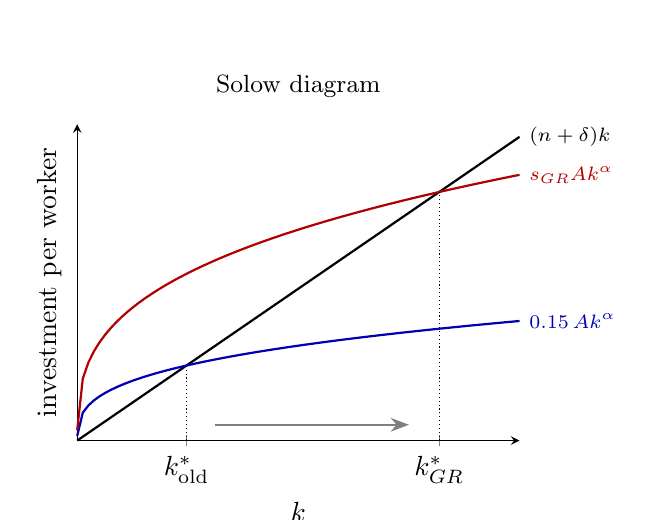
\begin{tikzpicture}
\begin{axis}[width=7.2cm,height=5.6cm,axis lines=left,xmin=0,xmax=16,ymin=0,ymax=1.0,
  xlabel={$k$},ylabel={investment per worker},xtick={3.953,13.095},xticklabels={$k^*_{\text{old}}$,$k^*_{GR}$},
  ytick=\empty,title={\small Solow diagram},clip=false]
\addplot[thick,black,domain=0:16,samples=60]{0.06*x};
\addplot[thick,blue!70!black,domain=0.001:16,samples=80]{0.15*x^(1/3)};
\addplot[thick,red!70!black,domain=0.001:16,samples=80]{(1/3)*x^(1/3)};
\addplot[densely dotted] coordinates {(3.953,0) (3.953,0.2372)};
\addplot[densely dotted] coordinates {(13.095,0) (13.095,0.7857)};
\node[font=\scriptsize,anchor=west] at (axis cs:16,0.96) {$(n+\delta)k$};
\node[font=\scriptsize,blue!70!black,anchor=west] at (axis cs:16,0.378) {$0.15\,Ak^{\alpha}$};
\node[font=\scriptsize,red!70!black,anchor=west] at (axis cs:16,0.84) {$s_{GR}Ak^{\alpha}$};
\draw[-{Stealth},thick,gray] (axis cs:5,0.05)--(axis cs:12,0.05);
\end{axis}
\end{tikzpicture}\quad
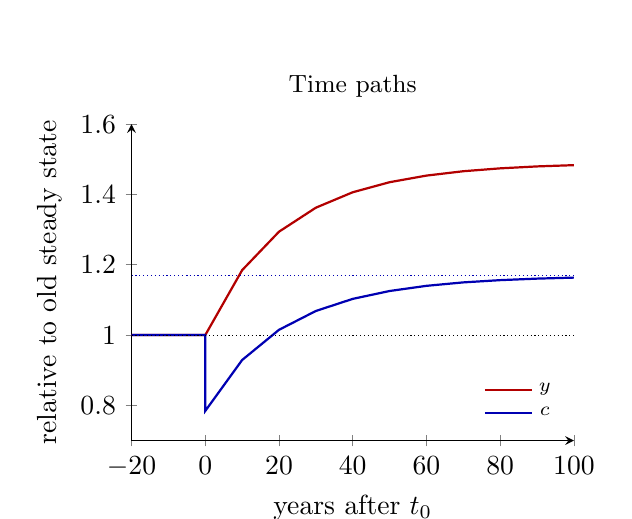
\begin{tikzpicture}
\begin{axis}[width=7.2cm,height=5.6cm,axis lines=left,xmin=-20,xmax=100,ymin=0.7,ymax=1.6,
  xlabel={years after $t_0$},ylabel={relative to old steady state},title={\small Time paths},
  legend style={font=\scriptsize,draw=none,at={(0.98,0.03)},anchor=south east}]
\addplot[thick,red!70!black] coordinates {(-20,1) (0,1) (10,1.1847) (20,1.2941) (30,1.3624) (40,1.4063)
  (50,1.4349) (60,1.4537) (70,1.4661) (80,1.4743) (90,1.4798) (100,1.4834)};
\addplot[thick,blue!70!black] coordinates {(-20,1) (0,1) (0,0.7843) (10,0.9291) (20,1.0150) (30,1.0686)
  (40,1.1030) (50,1.1254) (60,1.1401) (70,1.1499) (80,1.1563) (90,1.1606) (100,1.1635)};
\addplot[densely dotted,domain=-20:100]{1};
\addplot[densely dotted,blue!70!black,domain=-20:100]{1.1692};
\legend{$y$,$c$}
\end{axis}
\end{tikzpicture}
\end{center}
\passo{6 --- welfare}{Not necessarily. Brazil starts \emph{below} the golden rule ($0.15<1/3$), so the economy
is dynamically efficient and more steady-state consumption must be bought with less consumption during the
transition: current workers and retirees pay (21.6\% less consumption at once, below the old level for 18
years); later cohorts gain. Whether it is worth it depends on how the future is discounted --- an impatient
society optimally stays below $s_{GR}$ (compare optimal and fixed saving rates, Kurlat ex.~9.12, p.~185).
Only from \emph{above} $s_{GR}$ would a change (a cut in $s$) raise consumption at every date, a Pareto
improvement.}
\intuicao{A higher saving rate keeps raising output, but each extra unit of capital also needs $n+\delta$ of
replacement; past the point where MPK $=n+\delta$, capital costs more to maintain than it adds. With
Cobb--Douglas that point is reached exactly when the saving rate equals capital's income share.}
\refbib{Kurlat ch.~4, \S4.2 (steady state, pp.~59--61) and \S4.3 (golden rule, pp.~61--63); Jones (2020) ch.~5
for the transition paths.}
\rubrica{
\item (i) $k^*$ and $c^*$ with the exponent $\alpha/(1-\alpha)$: 0.15; $s_{GR}=\alpha$ derived: 0.1; MPK
cross-check: 0.1. Dropping the exponent (answer other than $\alpha$): max.\ 0.15 on (i). Maximising $k^*$ or
$y^*$ instead of $c^*$: 0 on (i).
\item (ii) Impact $-21.6\%$ with the reason (predetermined $k$): 0.1; $+16.9\%$ and $+49.1\%$: 0.15 (slip:
$-0.1$). Consumption rising on impact: 0 on that line.
\item (iii) Solow diagram with both curves and both crossings labelled: 0.1; time paths, $c$ jumping down and
$y$ not jumping: 0.1.
\item (iv) Trade-off and who pays: 0.1; why only above $s_{GR}$ is a change Pareto improving: 0.1.
}
\gap{Prova 01, 1.b--1.c (three approaches with all entries; what counts as investment) and 2.b (golden-rule
algebra: carry the exponent, cross-check with MPK $=n+\delta$).}
\end{sol}

% =============================================================================
\questao{(2.5 points) A labour tax: what it does depends on what the government does with the money.
\textnormal{\normalsize A one-period economy has a fixed capital stock $\bar K$, owned by the representative
household, which also owns the competitive firm. The household has one unit of time and utility
\eqref{q2:U}, with $\psi=1/3$. The firm produces \eqref{q2:F} with $\alpha=1/3$;
normalise $A\bar K^{\alpha}=1$. Labour income is taxed at rate $\tau$, so the household's budget is
\eqref{q2:BC}, where $T$ is a lump-sum transfer that the household takes as given:
\begin{align}
u &= \ln c+\psi\ln(1-L), \tag{U}\label{q2:U}\\
Y &= A\bar K^{\alpha}L^{1-\alpha}, \tag{F}\label{q2:F}\\
c &= (1-\tau)wL+r\bar K+\Pi+T. \tag{BC}\label{q2:BC}
\end{align}
Congress debates a 25\% tax on labour income.}}

\parte{a}{0.7 point} Let $\tau=T=0$. Write the household's and the firm's problems, their first-order
conditions and the market-clearing conditions; show that profits are zero, and find the equilibrium $L$, $Y$,
$w$ and $c$. Then solve the problem of a planner who chooses $c$ and $L$ subject only to technology, and show that
it gives the same allocation. State the theorem behind this and the assumptions it needs.
\resolespaco
\begin{sol}
\begin{notacao}
\item $c\ge0$: consumption. $L\in[0,1]$: hours worked; $1-L$: leisure (one unit of time).
\item $\psi>0$: weight of leisure in utility ($\psi=1/3$).
\item $Y$: output. $\bar K>0$: fixed capital stock. $A>0$: productivity, with $A\bar K^{\alpha}=1$.
$\alpha\in(0,1)$: capital's share ($\alpha=1/3$).
\item $w$, $r>0$: real wage and real rental rate of capital. $\Pi$: the firm's profit, paid to the household.
\item $\tau\in[0,1)$: tax rate on labour income. $T$: lump-sum transfer. In this item $\tau=T=0$.
\item $L_0$, $Y_0$, $w_0$, $c_0$: the equilibrium at $\tau=0$. $L^{P}$: the planner's choice.
\item MRS: marginal rate of substitution of leisure for consumption. MPL: marginal product of labour.
\end{notacao}
\passo{1 --- household}{With $\tau=T=0$, \eqref{q2:BC} is
\begin{equation}
c=wL+r\bar K+\Pi. \label{q2a:bc}
\end{equation}
Substitute \eqref{q2a:bc} into \eqref{q2:U}:
\[
\max_L\ \ln(wL+r\bar K+\Pi)+\psi\ln(1-L).
\]
Differentiate with respect to $L$ and set it to zero:
\[
\frac{w}{c}-\frac{\psi}{1-L}=0.
\]
Rearrange:
\begin{equation}
\boxed{\frac{\psi c}{1-L}=w} \label{q2a:hh}
\end{equation}
--- the marginal rate of substitution between leisure and consumption equals the real wage, the price of
leisure.}
\passo{2 --- firm}{The firm chooses $L$ and rents $\bar K$:
$\max\ A\bar K^{\alpha}L^{1-\alpha}-wL-r\bar K$. Differentiating \eqref{q2:F}:
\begin{align}
w &= (1-\alpha)A\bar K^{\alpha}L^{-\alpha}\nonumber\\
&= \frac{(1-\alpha)\big(A\bar K^{\alpha}L^{1-\alpha}\big)}{L}\nonumber\\
&= \frac{(1-\alpha)Y}{L}, \label{q2a:w}\\
r &= \alpha A\bar K^{\alpha-1}L^{1-\alpha}\nonumber\\
&= \frac{\alpha\big(A\bar K^{\alpha}L^{1-\alpha}\big)}{\bar K}\nonumber\\
&= \frac{\alpha Y}{\bar K}. \label{q2a:r}
\end{align}
Profits, using \eqref{q2a:w} and \eqref{q2a:r}:
\begin{align}
\Pi &= Y-wL-r\bar K\nonumber\\
&= Y-\left(\frac{(1-\alpha)Y}{L}\right)L-\left(\frac{\alpha Y}{\bar K}\right)\bar K\nonumber\\
&= Y-(1-\alpha)Y-\alpha Y\nonumber\\
&= \boxed{0} \label{q2a:pi}
\end{align}
(constant returns: factor payments exhaust output).}
\passo{3 --- clearing}{Labour: household supply $=$ firm demand; capital: $\bar K$; goods (no $G$):
\begin{equation}
c=Y. \label{q2a:goods}
\end{equation}}
\passo{4 --- solve}{Substitute \eqref{q2a:goods} and \eqref{q2a:w} into \eqref{q2a:hh}:
\begin{align*}
\frac{\psi\,(Y)}{1-L} &= \left(\frac{(1-\alpha)Y}{L}\right)\\
\psi L &= (1-\alpha)(1-L)\\
(1-\alpha+\psi)L &= 1-\alpha.
\end{align*}
Hence
\begin{align}
L_0 &= \boxed{\frac{1-\alpha}{1-\alpha+\psi}}\nonumber\\
&= \frac{1-\frac13}{1-\frac13+\frac13}\nonumber\\
&= \frac{2/3}{1}=\boxed{\tfrac23}. \label{q2a:L0}
\end{align}
Then, by \eqref{q2:F} with $A\bar K^{\alpha}=1$, \eqref{q2a:w}, \eqref{q2a:goods} and \eqref{q2a:r}:
\begin{align*}
Y_0 &= (2/3)^{2/3}=0.7631,\\
w_0 &= \frac{(2/3)(0.7631)}{2/3}=0.7631,\\
c_0 &= Y_0=0.7631,\\
r\bar K &= \alpha Y_0=\tfrac13(0.7631)=0.2544.
\end{align*}}
\passo{5 --- planner}{The planner substitutes technology \eqref{q2:F} into \eqref{q2:U}:
\begin{align}
\max_L\ \ln\!\big(A\bar K^{\alpha}L^{1-\alpha}\big)+\psi\ln(1-L)
=\text{const}+(1-\alpha)\ln L+\psi\ln(1-L). \label{q2a:plan}
\end{align}
Differentiate \eqref{q2a:plan} with respect to $L$:
\begin{equation}
\frac{1-\alpha}{L}=\frac{\psi}{1-L}. \label{q2a:planfoc}
\end{equation}
Cross-multiplying \eqref{q2a:planfoc} gives the second line of Step 4, so $L^{P}=\tfrac23$ (SOC: both terms
concave). The planner sets MRS $=$ MPL; the market sets MRS $=w$ \eqref{q2a:hh} and MPL $=w$ \eqref{q2a:w},
hence MRS $=$ MPL.}
\passo{6 --- theorem}{\textbf{First Welfare Theorem}: a competitive equilibrium is Pareto efficient, given
price-taking agents, complete markets, no externalities and no distortionary taxes. Here all hold at $\tau=0$.}
\refbib{Kurlat ch.~9, \S9.1--\S9.2, pp.~165--172 (equilibrium and the First Welfare Theorem); ch.~7, \S7.2,
pp.~131--137 (consumption--leisure choice).}
\rubrica{
\item Household FOC (MRS $=w$) and firm FOCs: 0.2. $\Pi=0$ shown: 0.1. Clearing conditions listed: 0.1.
\item $L_0=2/3$ with $Y,w,c$: 0.1 (slip: $-0.1$).
\item Planner's FOC and same allocation: 0.1. Theorem and its assumptions: 0.1.
\item Omitting capital income or profits from the budget: max.\ 0.4 on the item.
}
\end{sol}

\parte{b}{0.7 point} Now $\tau=25\%$ and the government returns the whole revenue as the transfer, so
$T=\tau wL$ in equilibrium. Find $L$ (in general and in numbers). Explain why returning the money does not undo
the effect of the tax. Show graphically, in the plane (leisure $\ell=1-L$, consumption $c$): the production
possibilities frontier, the equilibrium of (a), the new equilibrium, and the household's budget line at the new
equilibrium, with and without the transfer. Use the graph to explain why the new allocation is inefficient.
\resolespaco
\begin{sol}
\begin{notacao}
\item Symbols of (a) keep their meaning. New here:
\item $\tau=0.25$; $T=\tau wL$: the rebate, equal to the revenue in equilibrium, taken as given by the household.
\item $L_R$: hours under the rebated tax. $\ell\equiv1-L\in[0,1]$: leisure; $\ell_0$, $\ell_R$ at the two equilibria.
\item $E_0$, $E_R$: the equilibria of (a) and (b). $U_0$, $U_R$: the indifference curves through them.
\end{notacao}
\passo{1 --- FOC with the tax}{Substitute \eqref{q2:BC} into \eqref{q2:U}:
\[
\max_L\ \ln\big((1-\tau)wL+r\bar K+\Pi+T\big)+\psi\ln(1-L).
\]
Differentiate with respect to $L$, with $T$ taken as given, and set it to zero:
\[
\frac{(1-\tau)w}{c}-\frac{\psi}{1-L}=0.
\]
Rearrange, as in (a), now with $(1-\tau)w$ per hour:
\begin{equation}
\boxed{\frac{\psi c}{1-L}=(1-\tau)w}. \label{q2b:hh}
\end{equation}
$T$ does not appear: the household takes it as given, so it moves income, not the price of leisure.}
\passo{2 --- equilibrium}{The government returns the revenue:
\begin{equation}
T=\tau wL. \label{q2b:gov}
\end{equation}
Substitute \eqref{q2b:gov} into \eqref{q2:BC}, with $\Pi=0$ from \eqref{q2a:pi}, and then use \eqref{q2a:w} and
\eqref{q2a:r}:
\begin{align}
c &= (1-\tau)wL+r\bar K+(0)+(\tau wL)\nonumber\\
&= wL+r\bar K\nonumber\\
&= \left(\frac{(1-\alpha)Y}{L}\right)L+\left(\frac{\alpha Y}{\bar K}\right)\bar K\nonumber\\
&= (1-\alpha)Y+\alpha Y\nonumber\\
&= Y. \label{q2b:cY}
\end{align}
Substitute \eqref{q2b:cY} and \eqref{q2a:w} into \eqref{q2b:hh}:
\begin{align*}
\frac{\psi\,(Y)}{1-L} &= (1-\tau)\left(\frac{(1-\alpha)Y}{L}\right)\\
\psi L &= (1-\tau)(1-\alpha)(1-L).
\end{align*}
Solve for $L$:
\begin{equation}
\boxed{L_R=\frac{(1-\tau)(1-\alpha)}{\psi+(1-\tau)(1-\alpha)}}. \label{q2b:LR}
\end{equation}
Numbers: $(1-\tau)(1-\alpha)=0.75\cdot\tfrac23=0.5$, so
\[
L_R=\frac{0.5}{\frac13+0.5}=\frac{0.5}{0.8333}=\boxed{0.60}.
\]
Sign, differentiating \eqref{q2b:LR}:
\[
\frac{\partial L_R}{\partial\tau}=-\frac{\psi(1-\alpha)}{[\psi+(1-\tau)(1-\alpha)]^2}<0.
\]
The other variables, by \eqref{q2:F}, \eqref{q2a:w}, \eqref{q2b:gov}, \eqref{q2a:r} and \eqref{q2b:cY}:
\begin{align*}
Y &= 0.6^{2/3}=0.7114,\\
w &= \frac{(2/3)(0.7114)}{0.6}=0.7904,\\
(1-\tau)w &= 0.75(0.7904)=0.5928,\\
T &= 0.25(0.7904)(0.6)=0.1186=\tau(1-\alpha)Y,\\
r\bar K &= \alpha Y=\tfrac13(0.7114)=0.2371,\\
c &= Y=0.7114.
\end{align*}}
\passo{3 --- why the rebate does not undo it}{Each household compares one more hour with $(1-\tau)w$, not
with $w$: its own extra hour raises the transfer to \emph{everyone} by a negligible amount, so it ignores it.
In equilibrium the transfer returns the \emph{income} (\eqref{q2b:cY}: $c=Y$ exactly) but the \emph{price} of
leisure stays distorted. Combining \eqref{q2b:hh} with $w=\text{MPL}$ from \eqref{q2a:w}:
\#~a wedge, $\text{MRS}=(1-\tau)\,\text{MPL}<\text{MPL}$.}
\begin{center}
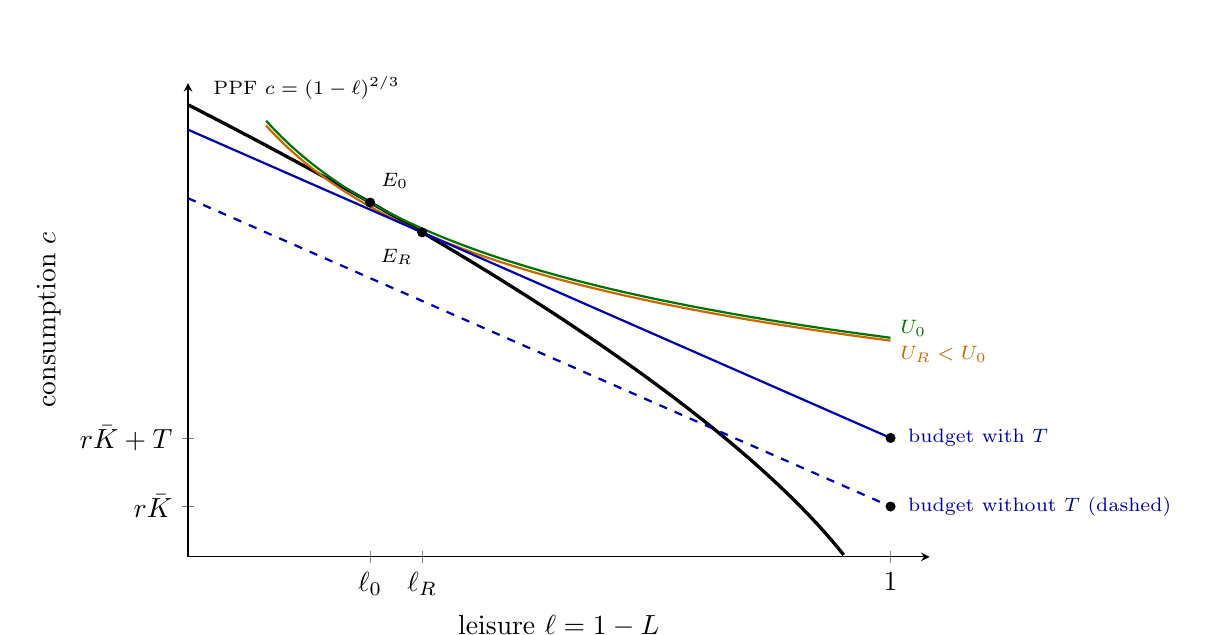
\begin{tikzpicture}
\begin{axis}[width=11cm,height=7.6cm,axis lines=left,xmin=0.1,xmax=1.05,ymin=0.15,ymax=0.97,clip=false,
  xlabel={leisure $\ell=1-L$},ylabel={consumption $c$},xtick={0.3333,0.4,1},xticklabels={$\ell_0$,$\ell_R$,$1$},
  ytick={0.2371,0.3557},yticklabels={$r\bar K$,$r\bar K+T$}]
\addplot[very thick,black,domain=0.1:0.94,samples=120]{(1-x)^(2/3)};
\addplot[thick,green!45!black,domain=0.2:1,samples=80]{0.52912*x^(-1/3)};
\addplot[thick,orange!80!black,domain=0.2:1,samples=80]{0.52418*x^(-1/3)};
\addplot[thick,blue!70!black,domain=0.1:1]{0.3557+0.5928*(1-x)};
\addplot[thick,blue!70!black,dashed,domain=0.1:1]{0.2371+0.5928*(1-x)};
\addplot[only marks,mark=*,mark size=1.6pt] coordinates {(0.3333,0.7631) (0.4,0.7114) (1,0.3557) (1,0.2371)};
\node[font=\scriptsize,anchor=south west] at (axis cs:0.335,0.77) {$E_0$};
\node[font=\scriptsize,anchor=north east] at (axis cs:0.40,0.70) {$E_R$};
\node[font=\scriptsize,anchor=south west] at (axis cs:0.12,0.925) {PPF $c=(1-\ell)^{2/3}$};
\node[font=\scriptsize,green!45!black,anchor=west] at (axis cs:1,0.545) {$U_0$};
\node[font=\scriptsize,orange!80!black,anchor=west] at (axis cs:1,0.50) {$U_R<U_0$};
\node[font=\scriptsize,blue!70!black,anchor=west] at (axis cs:1.01,0.3557) {budget with $T$};
\node[font=\scriptsize,blue!70!black,anchor=west] at (axis cs:1.01,0.2371) {budget without $T$ (dashed)};
\end{axis}
\end{tikzpicture}\\
{\footnotesize $E_0$: the indifference curve $U_0$ is tangent to the frontier (MRS $=$ MPL). $E_R$: the household is
tangent to its after-tax budget line (slope $(1-\tau)w=0.59$), which is flatter than the frontier there
(MPL $=w=0.79$), so the frontier \emph{crosses} $U_R$: there are feasible points above $U_R$. The tax rotates the
budget line about the no-work point $(1,r\bar K)$; the transfer shifts it up in parallel by $T$.}
\end{center}
\intuicao{The rebate gives the money back, but not the incentive: households still see 75 centavos for every real
their hour produces, so they buy too much leisure.}
\refbib{Kurlat ch.~7, \S7.2 (taxes and labour supply), pp.~131--137; related, not the same: ex.~7.5
\emph{Prescott's Calculation}, p.~148; ch.~9, \S9.2.}
\rubrica{
\item FOC with $(1-\tau)w$ and $c=Y$ from the government budget: 0.2. $L_R=0.6$ with the general formula and its
sign: 0.15 (slip: $-0.1$).
\item Why the transfer does not undo the wedge: 0.15. Claiming the rebate makes the tax neutral: max.\ 0.3 on the item.
\item Graph: axes, frontier, two indifference curves, tangency at $E_0$: 0.1; budget line rotated about the
no-work point and shifted by $T$, crossing argument at $E_R$: 0.1. Shifting the budget parallel for the tax: $-0.1$.
}
\end{sol}

\parte{c}{0.6 point} Instead, the same 25\% tax finances government purchases $G=\tau wL$ that give households
no utility ($T=0$). Find $L$. Using (a) and (b), split the change in hours relative to $\tau=0$ into a substitution
effect and an income effect, and explain why hours fall less than in (b). What happens if $\alpha=0$? An economist
argues: ``Labour taxes spent by the government barely change hours, so they cause almost no distortion.''
Evaluate, comparing with financing the same $G$ through a lump-sum tax.
\resolespaco
\begin{sol}
\begin{notacao}
\item Symbols of (a)--(b) keep their meaning. New here:
\item $G=\tau wL\ge0$: government purchases, which give no utility; now $T=0$.
\item $L_G$: hours when the tax finances $G$.
\item Substitution effect: change in $L$ from a change in the after-tax wage with income held fixed;
income effect: change in $L$ from the change in income alone.
\end{notacao}
\passo{1 --- equilibrium}{With $T=0$ and $\Pi=0$ \eqref{q2a:pi}, \eqref{q2:BC} becomes, using $wL+r\bar K=Y$
(Step 2 of (b)) and $wL=(1-\alpha)Y$ from \eqref{q2a:w}:
\begin{align}
c &= (1-\tau)wL+r\bar K+(0)+(0)\nonumber\\
&= (wL+r\bar K)-\tau wL\nonumber\\
&= (Y)-\tau wL\nonumber\\
&= Y-\tau\big((1-\alpha)Y\big)\nonumber\\
&= Y\,[1-\tau(1-\alpha)]. \label{q2c:c}
\end{align}
Numbers: $1-0.25\cdot\tfrac23=\tfrac56$, so $c=\tfrac56Y$ (goods clearing $c+G=Y$ gives the same).
The FOC \eqref{q2b:hh} still holds. Substitute \eqref{q2c:c} and \eqref{q2a:w} into it:
\begin{align*}
\frac{\psi\,\big([1-\tau(1-\alpha)]Y\big)}{1-L} &= (1-\tau)\left(\frac{(1-\alpha)Y}{L}\right)\\
\psi[1-\tau(1-\alpha)]\,L &= (1-\tau)(1-\alpha)(1-L).
\end{align*}
Solve for $L$:
\begin{equation}
\boxed{L_G=\frac{(1-\tau)(1-\alpha)}{\psi[1-\tau(1-\alpha)]+(1-\tau)(1-\alpha)}}. \label{q2c:LG}
\end{equation}
Numbers: $\psi[1-\tau(1-\alpha)]=\tfrac13\cdot\tfrac56=\tfrac{5}{18}$ and $(1-\tau)(1-\alpha)=0.5=\tfrac{9}{18}$:
\[
L_G=\frac{9/18}{\frac{5}{18}+\frac{9}{18}}=\boxed{\tfrac{9}{14}=0.643}.
\]
Then, by \eqref{q2:F}, \eqref{q2a:w} and \eqref{q2c:c}:
\begin{align*}
Y &= (9/14)^{2/3}=0.7449,\\
G &= \tau(1-\alpha)Y=\tfrac16(0.7449)=0.1241,\\
c &= \tfrac56(0.7449)=0.6207.
\end{align*}}
\passo{2 --- decomposition}{(b) changes the price of leisure but gives the income back: it isolates the
\textbf{substitution effect}. From \eqref{q2b:LR} and \eqref{q2a:L0}:
\[
L_R-L_0=0.600-0.667=\boxed{-0.067}.
\]
(c) has the same price change and also takes the income away: the step from (b) to (c) is the
\textbf{income effect}. From \eqref{q2c:LG} and \eqref{q2b:LR}:
\[
L_G-L_R=0.643-0.600=\boxed{+0.043}
\]
(poorer households buy less leisure, a normal good). Total:
\[
L_G-L_0=0.643-0.667=\boxed{-0.024}.
\]}
\passo{3 --- why less, and $\alpha=0$}{The two effects have opposite signs. With log utility they cancel only if
all income is taxed labour income. Here capital income $r\bar K$ is untaxed, so the income loss is smaller than
the price change: substitution wins and hours fall, but by less. Set $\alpha=0$ in \eqref{q2c:LG}:
\begin{align*}
L_G &= \frac{(1-\tau)(1-0)}{\psi[1-\tau(1-0)]+(1-\tau)(1-0)}\\
&= \frac{1-\tau}{\psi(1-\tau)+(1-\tau)}\\
&= \frac{1}{1+\psi},
\end{align*}
\textbf{independent of $\tau$}: exact cancellation.}
\passo{4 --- the economist}{Wrong. The distortion is the wedge MRS $=(1-\tau)$MPL, and its cost is driven by the
\emph{substitution} effect, not by the total response of hours. Benchmark: the same $G=0.1241$ raised lump-sum
leaves MRS $=$ MPL, so \eqref{q2a:hh} with $c=Y-G$ and \eqref{q2a:w} give
\begin{equation}
\frac{\psi(Y-G)}{1-L}=\frac{(1-\alpha)Y}{L}. \label{q2c:ls}
\end{equation}
Solving \eqref{q2c:ls} numerically gives $L=0.703$, more hours than at $\tau=0$ (pure income effect), and higher
utility: $-0.8104$ vs $-0.8201$, a consumption-equivalent gap of about $1.0\%$. Hours barely move under the
labour tax because two effects offset, not because nothing is distorted.}
\intuicao{The observer sees the total change in hours; welfare depends on the compensated change. A tax can leave
hours almost unchanged and still be costly, because it is the gap between what an hour produces and what it pays
that wastes resources.}
\refbib{Kurlat ch.~7, \S7.2 (income and substitution effects; log case), pp.~131--137; ch.~9, \S9.2.}
\rubrica{
\item $L_G=9/14$ with $c=Y[1-\tau(1-\alpha)]$: 0.2 (slip: $-0.1$).
\item Decomposition with signs and the reason (each effect named): 0.15. Reversing the labels: max.\ 0.1 on this line.
\item Why smaller here and the $\alpha=0$ case: 0.1.
\item Economist: wedge and compensated effect, with the lump-sum benchmark: 0.15. Conceding the claim: 0 on this line.
}
\end{sol}

\parte{d}{0.5 point} Return to the rebated tax of (b). Compute the welfare cost of the 25\% tax as the
percentage increase in consumption, at the allocation of (b), that would give households the utility of (a).
Show that the cost is of second order in $\tau$ (that a small tax has a much smaller cost) and check it with
$\tau=12.5\%$. Which instrument would avoid the cost?
\resolespaco
\begin{sol}
\begin{notacao}
\item Symbols of (a)--(b) keep their meaning. New here:
\item $U(L)$: utility as a function of hours when $c=Y$. $U_0$, $U_R$: its values in (a) and (b).
\item $\lambda\ge0$: welfare cost, the proportional rise in consumption at the allocation of (b) that gives
utility $U_0$.
\item $L_R(\tau)$: hours under the rebated tax as a function of $\tau$, from \eqref{q2b:LR}.
\end{notacao}
\passo{1 --- utility}{In both economies $c=Y$ (\eqref{q2a:goods}, \eqref{q2b:cY}) and, by \eqref{q2:F} with
$A\bar K^{\alpha}=1$, $Y=L^{2/3}$. Substitute into \eqref{q2:U}:
\begin{align}
U(L) &= \ln\big(L^{2/3}\big)+\tfrac13\ln(1-L)\nonumber\\
&= \tfrac23\ln L+\tfrac13\ln(1-L). \label{q2d:U}
\end{align}
Evaluate \eqref{q2d:U} at $L_0=\tfrac23$ and $L_R=0.6$:
\begin{align*}
U_0 &= \tfrac23\ln\tfrac23+\tfrac13\ln\tfrac13\\
&= (-0.27031)+(-0.36620)\\
&= -0.63651,\\
U_R &= \tfrac23\ln0.6+\tfrac13\ln0.4\\
&= (-0.34055)+(-0.30543)\\
&= -0.64598.
\end{align*}}
\passo{2 --- consumption equivalent}{By definition of $\lambda$:
\begin{equation}
\ln\big((1+\lambda)c_R\big)+\psi\ln(1-L_R)=U_0. \label{q2d:lam}
\end{equation}
Split the log in \eqref{q2d:lam} and use $U_R=\ln c_R+\psi\ln(1-L_R)$:
\begin{align*}
\ln(1+\lambda)+\big(\ln c_R+\psi\ln(1-L_R)\big) &= U_0\\
\ln(1+\lambda)+(U_R) &= U_0\\
\ln(1+\lambda) &= U_0-U_R\\
&= (-0.63651)-(-0.64598)\\
&= 0.00947,
\end{align*}
and $\lambda=e^{(0.00947)}-1=\boxed{0.95\%}$ of consumption.}
\passo{3 --- second order}{Welfare as a function of the tax is
\begin{equation}
U(\tau)=U\big(L_R(\tau)\big). \label{q2d:Utau}
\end{equation}
$L_0=L_R(0)$ maximises \eqref{q2d:U}: it is the planner's problem \eqref{q2a:plan}. Differentiate
\eqref{q2d:Utau} at $\tau=0$:
\begin{align*}
\frac{dU}{d\tau}\Big|_{\tau=0} &= U'(L_0)\,L_R'(0)\\
&= (0)\cdot L_R'(0)=0
\end{align*}
(envelope argument). The first-order term vanishes, and a second-order expansion of \eqref{q2d:Utau} leaves
\begin{equation}
U_0-U(\tau)\approx\tfrac12|U''(L_0)|\,[L_R'(0)]^2\tau^2, \label{q2d:harb}
\end{equation}
the Harberger triangle. Check: at $\tau=12.5\%$ the cost is $0.20\%$, about a fifth of $0.95\%$, close to the
quarter that \eqref{q2d:harb} predicts (the rest is higher-order terms).}
\passo{4 --- instrument}{A lump-sum tax (here, simply not taxing and not transferring): it does not touch the
marginal trade-off, so MRS $=$ MPL holds and the First Welfare Theorem applies again.}
\intuicao{At the efficient point the first hour moved has no value, so a small wedge costs almost nothing; the cost
grows with the square of the wedge, which is why many small taxes beat one large one.}
\refbib{Kurlat ch.~9, \S9.2 (welfare and taxes), pp.~168--172; ch.~7, \S7.2.}
\rubrica{
\item $U_0$, $U_R$ and $\lambda=0.95\%$: 0.2 (slip: $-0.1$). Comparing utils without converting: max.\ 0.1 on this line.
\item Envelope argument for the second-order cost: 0.15; $\tau=12.5\%$ check: 0.05.
\item Lump-sum tax as the first-best instrument: 0.1.
}
\gap{Kurlat ch.~7 and ch.~9 were absent from Prova 01; Prova 01, 2.c--2.d (list every income source, including
capital income and profits, and every choice variable).}
\end{sol}

% =============================================================================
\questao{(2.5 points) The Real plan, the trip to the bank and the inflation tax.
A stylised Brazil in the early 1990s. A representative household spends its real income $Y$ per year at a constant
rate. It keeps its wealth in an account that pays the nominal rate $i$ and withdraws cash $N$ times a year, in equal
amounts; cash pays no interest. Each trip to the bank costs $F$ in goods (queue, fee, time), that is $pF$ in money.
Take $Y=60{,}000$ (reais of constant purchasing power per year) and $F=25$. In the long run real output grows at
$g=4\%$ a year, the real interest rate is $r=3\%$ and the money supply grows at $\mu=11\%$ a year. Treat all money
as currency (money multiplier equal to one) and use Kurlat's Fisher equation $i=r+\pi$.}

\parte{a}{0.6 point} Derive the optimal number of trips $N$ and the demand for real money balances $M/p$ from the
household's cost minimisation. Find the income and interest elasticities of money demand and the velocity of
money. Compute $N$, $M/p$ and velocity at $i=12\%$. Show graphically how money demand depends on $i$, and how a
fall in $F$ (more ATMs) moves it.
\resolespaco
\begin{sol}
\begin{notacao}
\item $Y>0$: real income per year, spent at a constant rate ($Y=60{,}000$). $p>0$: price level.
\item $i>0$: nominal interest rate on the account; cash pays nothing.
\item $N>0$: withdrawals per year (an integer $\ge1$ in practice); $N^*$ the optimum.
\item $F>0$: real cost of one trip to the bank ($F=25$), so $pF$ in money.
\item $M$: average nominal cash held; $m\equiv M/p$: real money balances.
\item $\mathcal C(N)$: annual nominal cost of managing cash.
\item $\eta$: income elasticity of money demand. $V$: velocity of money.
\end{notacao}
\passo{1 --- the costs}{Each withdrawal is $pY/N$, spent at a constant rate down to zero, so average cash is
half of it:
\begin{equation}
M=\frac{pY}{2N}. \label{q3a:M}
\end{equation}
Annual cost: forgone interest on that cash plus the trips:
\begin{equation}
\mathcal C(N)=\frac{i\,pY}{2N}+pFN. \label{q3a:cost}
\end{equation}}
\passo{2 --- FOC}{Differentiate \eqref{q3a:cost} with respect to $N$ and set it to zero:
\begin{equation}
\mathcal C'(N)=-\frac{ipY}{2N^2}+pF=0. \label{q3a:foc}
\end{equation}
Solve \eqref{q3a:foc} for $N$:
\begin{equation}
\boxed{N^*=\sqrt{\frac{iY}{2F}}} \label{q3a:N}
\end{equation}
(SOC: $\mathcal C''=ipY/N^3>0$). Divide \eqref{q3a:M} by $p$ and substitute \eqref{q3a:N}:
\begin{align}
\frac{M}{p} &= \frac{Y}{2N^*}\nonumber\\
&= \frac{Y}{2\left(\sqrt{\frac{iY}{2F}}\right)}\nonumber\\
&= \frac{Y}{2}\sqrt{\frac{2F}{iY}}\nonumber\\
&= \sqrt{\frac{FY}{2i}}. \label{q3a:md}
\end{align}}
\passo{3 --- elasticities and velocity}{Take the log of \eqref{q3a:md}:
\begin{equation}
\ln\frac Mp=\tfrac12\ln\frac F2+\tfrac12\ln Y-\tfrac12\ln i. \label{q3a:ln}
\end{equation}
The coefficients in \eqref{q3a:ln} are the elasticities: income elasticity $\boxed{\eta=\tfrac12}$, interest
elasticity $\boxed{-\tfrac12}$ (economies of scale in cash management). Velocity, using the first line of
\eqref{q3a:md} and then \eqref{q3a:N}:
\begin{align}
V\equiv\frac{pY}{M} &= \frac{Y}{M/p}\nonumber\\
&= \frac{Y}{\left(\frac{Y}{2N^*}\right)}\nonumber\\
&= 2N^*\nonumber\\
&= 2\left(\sqrt{\frac{iY}{2F}}\right)\nonumber\\
&= \sqrt{\frac{2iY}{F}}: \label{q3a:V}
\end{align}
not a constant; it rises with $i$ and $Y$.}
\passo{4 --- numbers}{At $i=0.12$, by \eqref{q3a:N}, \eqref{q3a:md} and \eqref{q3a:V}:
\begin{align*}
N^* &= \sqrt{\frac{0.12\cdot60{,}000}{2\cdot25}}=\sqrt{144}=\boxed{12}\ \text{trips a year},\\
\frac Mp &= \frac{60{,}000}{2\cdot12}=\frac{60{,}000}{24}=\boxed{2{,}500},\\
V &= 2\cdot12=\boxed{24}.
\end{align*}}
\begin{center}
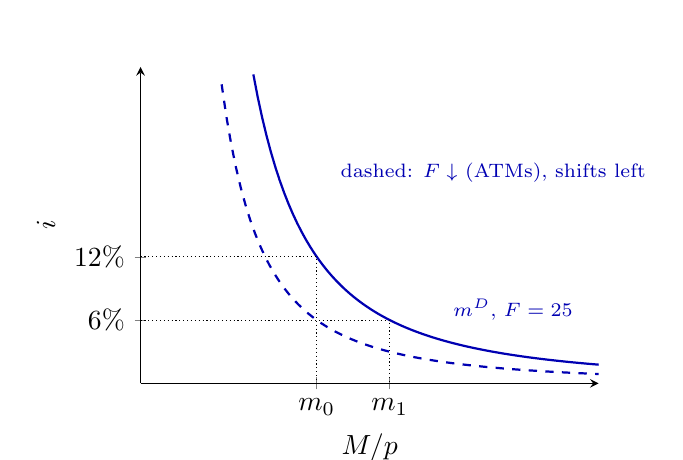
\begin{tikzpicture}
\begin{axis}[width=7.4cm,height=5.6cm,axis lines=left,xmin=0,xmax=6500,ymin=0,ymax=0.3,
  xlabel={$M/p$},ylabel={$i$},xtick={2500,3535.5},xticklabels={$m_0$,$m_1$},ytick={0.06,0.12},
  yticklabels={6\%,12\%},scaled x ticks=false,clip=false]
\addplot[thick,blue!70!black,domain=1600:6500,samples=80]{750000/x^2};
\addplot[thick,blue!70!black,dashed,domain=1150:6500,samples=80]{375000/x^2};
\addplot[densely dotted] coordinates {(0,0.12) (2500,0.12) (2500,0)};
\addplot[densely dotted] coordinates {(0,0.06) (3535.5,0.06) (3535.5,0)};
\node[font=\scriptsize,blue!70!black,anchor=west] at (axis cs:4300,0.07) {$m^D$, $F=25$};
\node[font=\scriptsize,blue!70!black,anchor=west] at (axis cs:2700,0.2) {dashed: $F\downarrow$ (ATMs), shifts left};
\end{axis}
\end{tikzpicture}
\end{center}
{\footnotesize Downward-sloping in $i$ (elasticity $-\tfrac12$); a lower $F$ shifts the whole curve left
(fewer balances at every $i$). Points used in (b): $i=12\%$ and $6\%$.}
\intuicao{Holding cash costs interest; refilling it costs trips. Doubling spending does not double cash, because the
trip cost is fixed: the optimal number of trips rises too.}
\refbib{Kurlat ch.~10, \S10.4, pp.~199--204, eqs.~(10.4.3)--(10.4.4); the exercise on ATMs, ex.~10.4, p.~203,
is related practice.}
\rubrica{
\item Average cash $pY/2N$ and the cost function: 0.15. $N^*$ and $M/p$ derived: 0.15.
\item Both elasticities and $V=2N$: 0.1. Numbers 12, 2{,}500, 24: 0.1 (slip: $-0.1$).
\item Graph with $i$ and $M/p$ on the axes and the shift for $F\downarrow$: 0.1.
\item Quoting $\sqrt{FY/2i}$ without deriving it: max.\ 0.2 on the item.
}
\end{sol}

\parte{b}{0.7 point} Using money-market equilibrium $M=p\,m^D(Y,i)$, derive the steady-state inflation rate when
$Y$ grows at $g$ and $i$ is constant, and compute $\pi$ and $i$. In mid-1994 the central bank cuts money growth
permanently and credibly to $\mu=5\%$. Find the new $\pi$ and $i$ and the change in real balances. Since the stock
of money does not jump by itself, what must happen to the price level on the day of the reform? Which one-time
change in $M$ would avoid it? Draw $\ln M$ and $\ln p$ around the reform, with that one-time change. A commentator
writes: ``After the Real, M1 rose by tens of percent while inflation collapsed, so money does not cause inflation.''
Evaluate.
\resolespaco
\begin{sol}
\begin{notacao}
\item Symbols of (a) keep their meaning. New here:
\item $m^D(Y,i)$: real money demand, \eqref{q3a:md}. A dot is a time derivative ($\dot M=dM/dt$).
\item $\mu\equiv\dot M/M$: money growth. $\pi\equiv\dot p/p$: inflation. $g\equiv\dot Y/Y$: real growth.
$r$: real interest rate. All per year.
\item $T$: date of the reform. $m_0$, $m_1$: real balances before and after; $p_{\text{old}}$, $p_{\text{new}}$:
price level just before and just after.
\end{notacao}
\passo{1 --- differentiate}{Money-market equilibrium at every date:
\begin{equation}
M_t=p_t\,m^D(Y_t,i_t). \label{q3b:mm}
\end{equation}
Differentiate \eqref{q3b:mm} with respect to $t$:
\begin{equation}
\dot M=\dot p\,m^D+p\Big(\frac{\partial m^D}{\partial Y}\dot Y+\frac{\partial m^D}{\partial i}\dot i\Big).
\label{q3b:diff}
\end{equation}
Set $\dot i=0$ and divide \eqref{q3b:diff} by \eqref{q3b:mm}:
\begin{align}
\frac{\dot M}{M} &= \frac{\dot p\,m^D+p\big(\frac{\partial m^D}{\partial Y}\dot Y+\frac{\partial m^D}{\partial i}(0)\big)}{p\,m^D}
\nonumber\\
&= \frac{\dot p}{p}+\underbrace{\frac{\partial m^D}{\partial Y}\frac{Y}{m^D}}_{\eta}
\frac{\dot Y}{Y}\nonumber\\
\mu &= \pi+\eta g\nonumber\\
\pi &= \mu-\eta g, \label{q3b:pi}
\end{align}
with $\eta=\tfrac12$ from \eqref{q3a:ln}. Kurlat's Fisher equation, from the statement:
\begin{equation}
i=r+\pi. \label{q3b:fisher}
\end{equation}}
\passo{2 --- before}{By \eqref{q3b:pi} and then \eqref{q3b:fisher}:
\begin{align*}
\pi &= 11\%-\tfrac12(4\%)=\boxed{9\%},\\
i &= 3\%+9\%=\boxed{12\%}
\end{align*}
(exact Fisher: $1.03\cdot1.09-1=12.27\%$).}
\passo{3 --- after}{With $\mu=5\%$, by \eqref{q3b:pi} and \eqref{q3b:fisher}:
\begin{align*}
\pi &= 5\%-\tfrac12(4\%)=\boxed{3\%},\\
i &= 3\%+3\%=\boxed{6\%}
\end{align*}
(Fisher effect: $i$ falls one-for-one with $\pi$, $r$ unchanged). Real balances, from the ratio of
\eqref{q3a:md} at the two rates:
\begin{align*}
\frac{m_1}{m_0} &= \frac{\sqrt{FY/(2i_1)}}{\sqrt{FY/(2i_0)}}\\
&= \sqrt{\frac{i_0}{i_1}}\\
&= \sqrt{\frac{0.12}{0.06}}\\
&= \sqrt2=1.414,
\end{align*}
$\boxed{+41.4\%}$ ($2{,}500\to3{,}536$). The jump is immediate: a credible reform changes expected inflation,
hence $i$, at once.}
\passo{4 --- the price level}{Solve \eqref{q3b:mm} for the price level:
\begin{equation}
p=\frac{M}{m^D}. \label{q3b:p}
\end{equation}
If $M$ is continuous and $m^D$ jumps by $\sqrt2$, \eqref{q3b:p} makes $p$ jump \emph{down}:
\begin{align*}
\frac{p_{\text{new}}}{p_{\text{old}}} &= \frac{M/m_1}{M/m_0}\\
&= \frac{m_0}{m_1}\\
&= \frac{1}{\sqrt2}=0.707,
\end{align*}
a $\boxed{29.3\%}$ fall in the price level. To keep $p$ continuous in \eqref{q3b:p}, $M$ must jump with $m^D$:
the central bank issues a one-time injection
\[
\boxed{\frac{\Delta M}{M}=\sqrt2-1=41.4\%}
\]
on the day of the reform (remonetisation), and \emph{from then on} money grows at 5\%. This injection is not
inflationary: it only meets the higher demand for real balances.}
\begin{center}
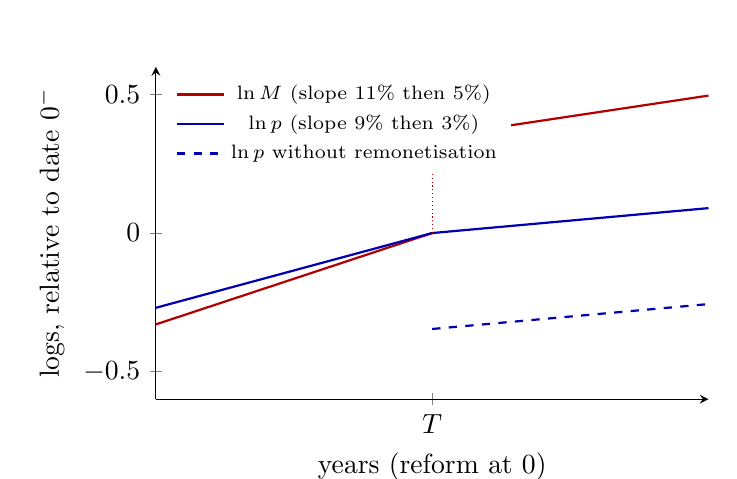
\begin{tikzpicture}
\begin{axis}[width=8.6cm,height=5.8cm,axis lines=left,xmin=-3,xmax=3,ymin=-0.6,ymax=0.6,
  xlabel={years (reform at $0$)},ylabel={logs, relative to date $0^-$},xtick={0},xticklabels={$T$},
  legend style={font=\scriptsize,draw=none,at={(0.02,0.98)},anchor=north west}]
\addplot[thick,red!70!black] coordinates {(-3,-0.33) (0,0)};
\addplot[thick,blue!70!black] coordinates {(-3,-0.27) (0,0)};
\addplot[thick,blue!70!black,dashed] coordinates {(0,-0.3466) (3,-0.2566)};
\addplot[thick,red!70!black,forget plot] coordinates {(0,0.3466) (3,0.4966)};
\addplot[thick,blue!70!black,forget plot] coordinates {(0,0) (3,0.09)};
\addplot[densely dotted,red!70!black,forget plot] coordinates {(0,0) (0,0.3466)};
\legend{$\ln M$ (slope 11\% then 5\%),$\ln p$ (slope 9\% then 3\%),$\ln p$ without remonetisation}
\end{axis}
\end{tikzpicture}\\
{\footnotesize With remonetisation $\ln M$ jumps by $\ln\sqrt2=0.35$ and $\ln p$ only changes slope. Without it,
$\ln M$ is continuous and $\ln p$ jumps down by $0.35$.}
\end{center}
\passo{5 --- the commentator}{Wrong inference. \eqref{q3b:pi} holds \emph{with $i$ constant}; at the reform $i$
falls and real money demand rises by about 41\%, so a one-time rise in $M$ of that size is exactly what keeps
prices stable. It is a \emph{level} adjustment of $M$ to a higher $m^D$, not sustained money growth. The theory
predicts both facts at once: the money stock jumps and inflation falls, because $\mu$ after the jump is low.}
\intuicao{When people expect inflation to fall, holding cash becomes cheaper and they want more of it. Either the
central bank supplies that cash, or prices fall until existing cash is worth enough.}
\refbib{Kurlat ch.~11, \S11.2, pp.~209--212, eq.~(11.2.3); \S11.1--\S11.2 on neutrality, pp.~205--215.}
\rubrica{
\item Total differentiation with $\dot i=0$ stated and $\eta$ named: 0.15. $\pi=9\%$, $i=12\%$: 0.05.
\item $\pi=3\%$, $i=6\%$, $m$ up by $\sqrt2$: 0.15. Using $\eta=1$ (quantity theory) instead of $\tfrac12$: $-0.1$.
\item Price-level jump of $-29.3\%$ or remonetisation of $41.4\%$: 0.15. Graph (slopes and the jump): 0.1.
\item Commentator: level vs growth, $m^D$ rising with lower $i$: 0.1. Agreeing with the commentator: 0 on this line.
}
\end{sol}

\parte{c}{0.6 point} Seigniorage. Compute real seigniorage per household before and after the reform, and split it
into the inflation tax and the part due to growth. Show that with the money demand of (a) seigniorage rises with
$\mu$ for every $\mu$, so there is no revenue-maximising money growth. Contrast with a Cagan semi-log demand
$M/p=Y e^{-a i}$, $a>0$: find the revenue-maximising $\mu$ and evaluate it for $a=2$. Draw both curves. Which demand
is consistent with Brazil's 1989--1993 experience, when money grew by more than 1{,}000\% a year?
\resolespaco
\begin{sol}
\begin{notacao}
\item Symbols of (a)--(b) keep their meaning. New here:
\item $S$: real seigniorage per household per year, the real value of newly issued money.
\item $a>0$: semi-elasticity of the Cagan demand $M/p=Ye^{-ai}$ with respect to $i$ ($a=2$).
\item $\mu^{\max}$: the money growth that maximises $S$ (the peak of the seigniorage Laffer curve).
\end{notacao}
\passo{1 --- definition}{Real seigniorage, multiplying and dividing by $M$:
\begin{align}
S\equiv\frac{\dot M}{p} &= \frac{\dot M}{M}\cdot\frac{M}{p}\nonumber\\
&= \mu\,m. \label{q3c:S}
\end{align}
Substitute $\mu=\pi+\eta g$ from \eqref{q3b:pi} into \eqref{q3c:S}:
\begin{align}
S &= (\pi+\eta g)\,m\nonumber\\
&= \underbrace{\pi m}_{\text{inflation tax}}+\underbrace{\eta g\,m}_{\text{growth}}. \label{q3c:split}
\end{align}}
\passo{2 --- numbers}{Before ($\mu=11\%$, $\pi=9\%$, $m=2{,}500$), by \eqref{q3c:S} and \eqref{q3c:split}:
\begin{align*}
S &= 0.11\cdot2{,}500=\boxed{275},\\
\pi m+\eta g\,m &= 0.09\cdot2{,}500+\tfrac12(0.04)\cdot2{,}500=225+50,
\end{align*}
$0.46\%$ of $Y$. After ($\mu=5\%$, $\pi=3\%$, $m=3{,}536$):
\begin{align*}
S &= 0.05\cdot3{,}536=\boxed{176.8},\\
\pi m+\eta g\,m &= 0.03\cdot3{,}536+\tfrac12(0.04)\cdot3{,}536=106.1+70.7,
\end{align*}
$0.29\%$ of $Y$. Revenue falls by 36\%, much less than $\mu$ (by 55\%), because the base rises 41\%; and the
growth part \emph{rises}: a growing economy absorbs new money without inflation.}
\passo{3 --- no peak under Baumol--Tobin}{Substitute \eqref{q3b:pi} into \eqref{q3b:fisher}:
\begin{align}
i &= r+(\mu-\eta g)\nonumber\\
&= 0.03+\mu-\tfrac12(0.04)\nonumber\\
&= \mu+0.01. \label{q3c:i}
\end{align}
Substitute \eqref{q3a:md} with \eqref{q3c:i} into \eqref{q3c:S}:
\begin{align}
S &= \mu\left(\sqrt{\frac{FY}{2i}}\right)\nonumber\\
S(\mu) &= \mu\sqrt{\frac{FY}{2(\mu+r-\eta g)}}. \label{q3c:Sbt}
\end{align}
Differentiate the log of \eqref{q3c:Sbt}, using $di/d\mu=1$ and $2i-\mu=\mu+2(r-\eta g)$:
\begin{align*}
\frac{d\ln S}{d\mu} &= \frac1\mu-\frac{1}{2i}\\
&= \frac{2i-\mu}{2\mu i}\\
&= \frac{2(\mu+r-\eta g)-\mu}{2\mu i}\\
&= \frac{\mu+2(r-\eta g)}{2\mu i}>0
\end{align*}
for all $\mu>0$, since $r-\eta g=1\%>0$. Equivalently, the elasticity of the base with respect to $\mu$ is $-\mu/(2i)>-\tfrac12>-1$: the base never shrinks
fast enough to offset the rate. \#~The Laffer peak needs a base elasticity of $-1$.}
\passo{4 --- Cagan}{The Cagan demand:
\begin{equation}
\frac Mp=Ye^{-ai}. \label{q3c:cagan}
\end{equation}
Substitute \eqref{q3c:cagan} with \eqref{q3c:i} into \eqref{q3c:S}:
\begin{align}
S &= \mu\big(Ye^{-ai}\big)\nonumber\\
&= \mu Y e^{-a(r-\eta g+\mu)}. \label{q3c:Scagan}
\end{align}
Differentiate \eqref{q3c:Scagan} with respect to $\mu$ and set it to zero:
\begin{align*}
\frac{dS}{d\mu} &= Ye^{-a(\cdot)}\,(1-a\mu)=0\\
\Rightarrow\ \mu^{\max} &= 1/a.
\end{align*}
SOC: $\frac{d^2S}{d\mu^2}=-aYe^{-a(\cdot)}(2-a\mu)<0$ at $\mu=1/a$. With $a=2$:
$\boxed{\mu^{\max}=1/a=1/2=50\%}$ a year.}
\begin{center}
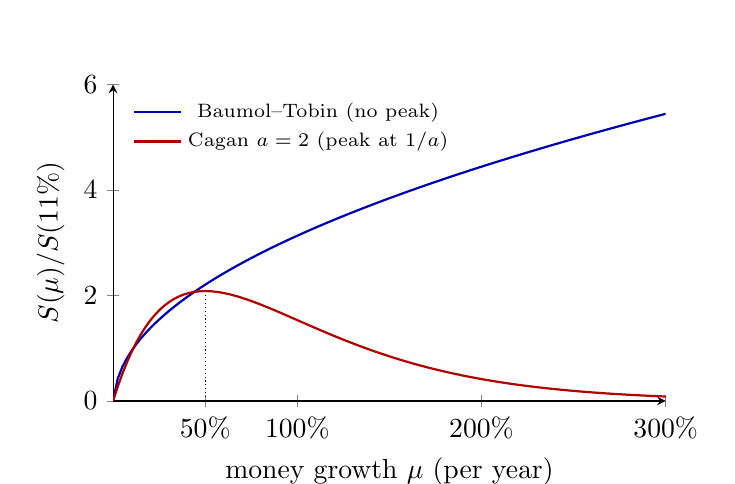
\begin{tikzpicture}
\begin{axis}[width=8.6cm,height=5.6cm,axis lines=left,xmin=0,xmax=3,ymin=0,ymax=6,
  xlabel={money growth $\mu$ (per year)},ylabel={$S(\mu)/S(11\%)$},xtick={0.5,1,2,3},
  xticklabels={50\%,100\%,200\%,300\%},
  legend style={font=\scriptsize,draw=none,at={(0.02,0.98)},anchor=north west}]
\addplot[thick,blue!70!black,domain=0:3,samples=120]{x/sqrt(x+0.01)/0.31754};
\addplot[thick,red!70!black,domain=0:3,samples=120]{x*exp(-2*(x+0.01))/0.086530};
\addplot[densely dotted] coordinates {(0.5,0) (0.5,2.0837)};
\legend{Baumol--Tobin (no peak),Cagan $a=2$ (peak at $1/a$)}
\end{axis}
\end{tikzpicture}
\end{center}
\passo{5 --- Brazil}{Rising revenue at any $\mu$, as \eqref{q3c:Sbt} implies, cannot explain why governments
printing over 1{,}000\% a year did not raise ever more revenue; with a Cagan demand \eqref{q3c:Scagan} they were
far on the \emph{wrong side} of the Laffer curve, where cutting $\mu$ costs little revenue or even raises it.
Baumol--Tobin with a fixed $F$ misses the flight from money at high inflation (indexed overnight accounts lowered
the effective $F$ and made demand far more elastic).}
\intuicao{Seigniorage is a tax with rate $\mu$ on the base $M/p$. Whether raising the rate raises revenue depends on
how fast the base flees; under Baumol--Tobin it flees too slowly to ever turn revenue down.}
\refbib{Kurlat ch.~11, \S11.3, pp.~215--216 (seigniorage); the Cagan demand is used in ex.~11.6, p.~218, which
works the limit on revenue with another functional form.}
\rubrica{
\item $S=\mu m$ and the split: 0.1. Both numbers and splits: 0.15 (slip: $-0.1$).
\item Proof of no peak (derivative signed, or elasticity $>-1$): 0.15. Asserting it without proof: 0 on this line.
\item Cagan peak with SOC and 50\%: 0.1. Graph (both curves, peak marked): 0.05.
\item Brazil reading: 0.05.
}
\end{sol}

\parte{d}{0.6 point} Costs of inflation. Compute the real resources spent on trips to the bank, in reais and as a
share of $Y$, before and after the reform. Why is the forgone interest on cash not counted as a cost to society?
Find the inflation and money-growth rates of the Friedman rule, and say what happens to the Baumol--Tobin solution
there. Give two reasons why the central bank targets 3\% rather than this rate.
\resolespaco
\begin{sol}
\begin{notacao}
\item Symbols of (a)--(c) keep their meaning. New here:
\item $R\ge0$: real resources spent on trips to the bank per year (shoe-leather cost), $R=FN^*$.
\item Friedman rule: the policy that sets the nominal interest rate to zero, $i=0$.
\end{notacao}
\passo{1 --- trips}{The resource cost is the number of trips times their real cost. Substitute
\eqref{q3a:N}:
\begin{align}
R=FN^* &= F\left(\sqrt{\frac{iY}{2F}}\right)\nonumber\\
&= \boxed{\sqrt{\frac{iFY}{2}}}. \label{q3d:R}
\end{align}
Before ($i=12\%$, $N^*=12$) and after ($i=6\%$), by \eqref{q3d:R}:
\begin{align*}
R_{\text{before}} &= 25\cdot12=\boxed{300},\quad 0.50\%\ \text{of }Y,\\
R_{\text{after}} &= \sqrt{\frac{0.06\cdot25\cdot60{,}000}{2}}=\sqrt{45{,}000}=\boxed{212.1},\quad 0.35\%\ \text{of }Y.
\end{align*}
The reform saves $0.15\%$ of income every year (shoe-leather cost).}
\passo{2 --- forgone interest}{Multiply \eqref{q3a:md} by $i$: at the optimum the forgone interest is
\[
i\,\frac Mp=i\left(\sqrt{\frac{FY}{2i}}\right)=\sqrt{\frac{iFY}{2}},
\]
the same as \eqref{q3d:R} (300 before), but it is not a use of resources: the inflation-tax part
($\pi m=225$, \eqref{q3c:split}) is revenue of the government, and the rest is a transfer to whoever borrows the
funds. Only the trips burn goods. (Total private cost $\sqrt{2iFY}=600$.)}
\passo{3 --- Friedman rule}{Set $i=0$ in \eqref{q3b:fisher}, then use \eqref{q3b:pi} solved for $\mu$:
\begin{align*}
(0) &= r+\pi\\
\pi &= -r=\boxed{-3\%},\\
\mu &= \pi+\eta g=(-3\%)+\tfrac12(4\%)=\boxed{-1\%}.
\end{align*}
Then, by \eqref{q3a:N} and \eqref{q3a:md}, $N^*\to0$ and $M/p\to\infty$. The interior solution needs $N^*\ge1$;
by \eqref{q3a:N}:
\[
\frac{iY}{2F}\ge1\iff i\ge\frac{2F}{Y}=\frac{2\cdot25}{60{,}000}=0.083\%;
\]
below that the household makes one trip and holds $Y/2=30{,}000$. Shoe-leather costs vanish.}
\passo{4 --- why 3\%}{(i) Measured inflation overstates true inflation (substitution, quality and new-goods biases
of a Laspeyres index), so 0 measured is deflation. (ii) With $\pi=-3\%$, $i$ would sit at zero in normal times,
leaving no room to cut it in a recession --- the zero lower bound of Question 4. (iii) Nominal wages are rigid
downward; some inflation lets real wages fall.}
\intuicao{Inflation is a tax on holding cash; people spend real resources dodging it. The Friedman rule removes the
tax, but a central bank that needs room to cut rates gives up a little of that gain.}
\refbib{Kurlat ch.~11, \S11.4, pp.~216--222 (costs of inflation, Friedman rule); ch.~10, \S10.4.}
\rubrica{
\item Trip cost formula and both numbers with shares: 0.2 (slip: $-0.1$). Counting $i\,m$ as the social cost: max.\ 0.1 on this line.
\item Transfer argument: 0.1. Friedman rule $\pi=-3\%$, $\mu=-1\%$: 0.1; the corner $N\ge1$: 0.05.
\item Two valid reasons for a positive target: 0.15.
}
\gap{Kurlat ch.~10--11 were absent from Prova 01: Baumol--Tobin from primitives, $\pi=\mu-\eta g$ by total
differentiation, Fisher, seigniorage and its Laffer curve.}
\end{sol}

% =============================================================================
\questao{(3.0 points) The Copom between a tax shock and a liquidity trap.
Use Benigno (2015), in log deviations from an efficient steady state, with a short run and a long run:
\begin{align}
y &= \bar y_n+(g-\bar g)-\sigma\left[i-(\bar p-p)-\rho\right], \tag{AD}\label{q4:AD}\\
p-p^e &= \kappa(y-y_n), \tag{AS}\label{q4:AS}\\
y_n &= \frac{(1+\eta)a+\sigma^{-1}g-\mu}{\sigma^{-1}+\eta}, \tag{YN}\label{q4:YN}\\
y_e &= \frac{(1+\eta)a+\sigma^{-1}g}{\sigma^{-1}+\eta}. \tag{YE}\label{q4:YE}
\end{align}
Initially $a=g=\bar g=\mu=0$, $\bar y_n=0$, $\bar p=p^e=0$ and $i=\rho$. Take $\sigma=1$, $\eta=1$, $\kappa=1/2$ and
$\rho=2\%$; $y$ and $p$ are in percent. The Copom sets $i$ to minimise
\begin{equation}
L=\tfrac12(y-y_e)^2+\frac{\phi}{2\kappa}(p-p^e)^2,\qquad \phi>0. \tag{LF}\label{q4:LF}
\end{equation}}

\parte{a}{0.8 point} A temporary rise in a federal tax on firms' revenues raises the mark-up by $\mu=4$ in the
current period only. Find the changes in $y_n$ and $y_e$ and say which curve shifts. Derive the Copom's optimal
targeting rule by substituting the relevant constraint into the loss, and the optimal $y$ and $p$ as functions of
$\phi$; evaluate them for $\phi=4$. Explain why the Copom cannot reach $y=y_e$ and $p=p^e$ together here, while it
could after a temporary productivity shock. Show graphically.
\resolespaco
\begin{sol}
\begin{notacao}
\item $y$, $p$: output and price level today, log deviations from the steady state, in percent.
\item $\bar y_n$, $\bar p$: long-run natural output and long-run price level. $p^e$: the price preset by firms
that cannot adjust this period.
\item $i\ge0$: nominal policy rate, the Copom's instrument. $\rho>0$: rate of time preference, the steady-state
real rate ($\rho=2\%$).
\item $g$, $\bar g$: government spending today and in the long run. $a$: productivity. $\mu$: firms' mark-up
(here raised by the tax).
\item $\sigma>0$: intertemporal elasticity of substitution (not the capital share of Q1). $\eta>0$: inverse
Frisch elasticity of labour supply. $\kappa>0$: slope of AS.
\item $y_n$: natural output (flexible prices, with the mark-up). $y_e$: efficient output (no mark-up).
\item $\phi>0$: weight on price surprises in the loss $L$ \eqref{q4:LF}.
\item $\Delta\equiv y_e-y_n$: the gap between efficient and natural output (defined in Step 1).
\item $y^*$, $p^*$: the optimal point. $E_0$: initial equilibrium. $E'$: the outcome with $i=\rho$. $O$: the optimum.
\end{notacao}
\passo{1 --- what moves}{Differentiate \eqref{q4:YN} and \eqref{q4:YE} with respect to $\mu$:
\begin{align}
dy_n &= -\frac{\mu}{\sigma^{-1}+\eta}=-\frac{4}{1+1}=\boxed{-2}, \label{q4a:dyn}\\
dy_e &= \boxed{0}\qquad(\mu\text{ is not in }y_e). \label{q4a:dye}
\end{align}
\textbf{AS shifts up/left}: by \eqref{q4:AS} it now passes through $(y_n',p^e)=(-2,0)$, so at each $y$ the price
is higher by $\kappa\cdot2=1$. \textbf{AD does not move}: $\mu$ is not in \eqref{q4:AD} and, the shock being
temporary, $\bar y_n$ is unchanged. From \eqref{q4a:dyn}--\eqref{q4a:dye}:
\begin{equation}
\Delta\equiv y_e-y_n=0-(-2)=2>0. \label{q4a:Delta}
\end{equation}}
\passo{2 --- the constraint}{The Copom moves AD with $i$, so it can pick \emph{any} point on AS; AS ($p^e$ is
predetermined) is the constraint. Substitute \eqref{q4:AS} into \eqref{q4:LF}:
\begin{align}
L(y) &= \tfrac12(y-y_e)^2+\frac{\phi}{2\kappa}\big(\kappa(y-y_n)\big)^2\nonumber\\
&= \tfrac12(y-y_e)^2+\frac{\phi}{2\kappa}\kappa^2(y-y_n)^2\nonumber\\
&= \tfrac12(y-y_e)^2+\frac{\phi\kappa}{2}(y-y_n)^2. \label{q4a:Ly}
\end{align}}
\passo{3 --- targeting rule}{Differentiate \eqref{q4a:Ly} and set it to zero (SOC $1+\phi\kappa>0$):
\begin{equation}
\frac{dL}{dy}=(y-y_e)+\phi\kappa(y-y_n)=0. \label{q4a:foc}
\end{equation}
By \eqref{q4:AS}, $\kappa(y-y_n)=p-p^e$. Substitute this into \eqref{q4a:foc}:
\begin{equation}
\boxed{(y-y_e)+\phi\,(p-p^e)=0}. \label{q4a:rule}
\end{equation}
Solve \eqref{q4a:foc} for $y$, then use $y_e=0$ and $y_n=-\Delta$ from \eqref{q4a:Delta}:
\begin{align}
y(1+\phi\kappa) &= y_e+\phi\kappa\,y_n\nonumber\\
y^* &= \frac{y_e+\phi\kappa\,y_n}{1+\phi\kappa}\nonumber\\
&= \frac{(0)+\phi\kappa\,(-\Delta)}{1+\phi\kappa}\nonumber\\
&= -\frac{\phi\kappa\,\Delta}{1+\phi\kappa}. \label{q4a:ystar}
\end{align}
Subtract $y_n=-\Delta$ from \eqref{q4a:ystar} and substitute into \eqref{q4:AS}:
\begin{align}
y^*-y_n &= \left(-\frac{\phi\kappa\,\Delta}{1+\phi\kappa}\right)-(-\Delta)\nonumber\\
&= \frac{\Delta}{1+\phi\kappa},\nonumber\\
p^*-p^e &= \kappa(y^*-y_n)\nonumber\\
&= \kappa\left(\frac{\Delta}{1+\phi\kappa}\right)\nonumber\\
&= \frac{\kappa\,\Delta}{1+\phi\kappa}. \label{q4a:pstar}
\end{align}
With $\phi=4$, $\phi\kappa=2$; by \eqref{q4a:ystar} and \eqref{q4a:pstar}:
\begin{align*}
y^* &= -\frac{2\cdot2}{1+2}=\boxed{-1.33\%},\\
p^* &= \frac{0.5\cdot2}{1+2}=\boxed{+0.33\%}.
\end{align*}
Check in \eqref{q4a:rule}: $-\tfrac43+4\cdot\tfrac13=0$ \checkmark.}
\passo{4 --- divine coincidence fails}{Both targets require $y=y_e=0$ and $p=p^e$, but on the new AS
\eqref{q4:AS}, $p-p^e=\kappa(0+2)=1\neq0$ at $y=0$: the bliss point is not on the constraint, and one instrument
cannot hit two targets. After a temporary productivity shock, \eqref{q4:YN} and \eqref{q4:YE} move $y_n$ and $y_e$
by the same $\frac{1+\eta}{\sigma^{-1}+\eta}a$, so $(y_e,p^e)$ lies on the new AS and the Copom puts AD through it:
zero loss, whatever $\phi$.}
\begin{center}
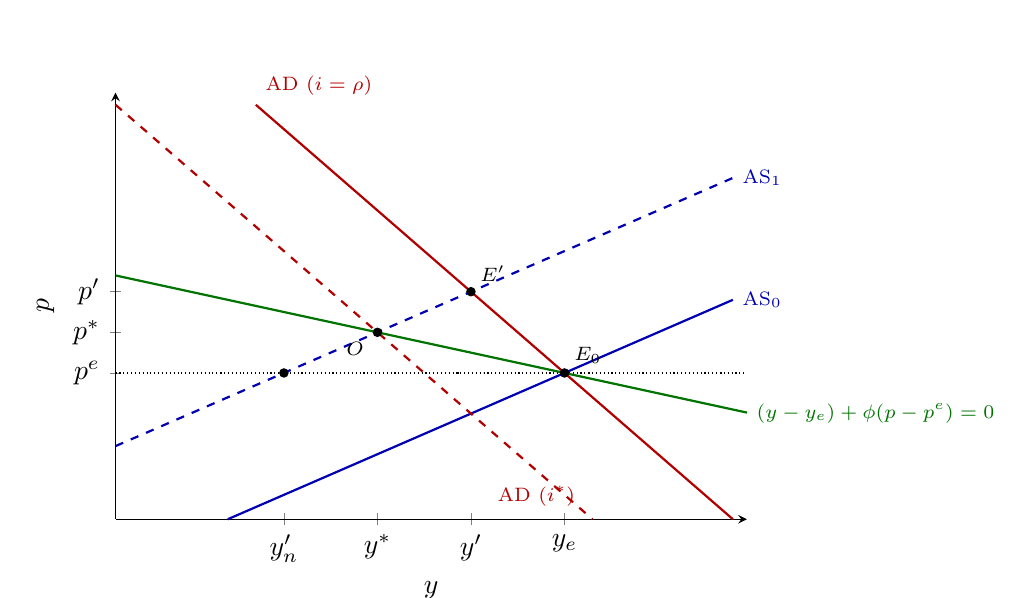
\begin{tikzpicture}
\begin{axis}[width=9.6cm,height=7cm,axis lines=left,xmin=-3.2,xmax=1.3,ymin=-1.2,ymax=2.3,clip=false,
  xlabel={$y$},ylabel={$p$},
  xtick={-2,-1.3333,-0.6667,0},xticklabels={$y_n'$,$y^*$,$y'$,$y_e$},ytick={0,0.3333,0.6667},
  yticklabels={$p^e$,$p^*$,$p'$}]
\addplot[densely dotted,domain=-3.2:1.3]{0};
\addplot[thick,blue!70!black,domain=-2.4:1.2]{0.5*x};
\addplot[thick,blue!70!black,dashed,domain=-3.2:1.2]{0.5*(x+2)};
\addplot[thick,red!70!black,domain=-2.2:1.2]{-x};
\addplot[thick,red!70!black,dashed,domain=-3.2:0.2]{-x-1};
\addplot[thick,green!45!black,domain=-3.2:1.3]{-x/4};
\addplot[only marks,mark=*,mark size=1.5pt] coordinates {(0,0) (-0.6667,0.6667) (-1.3333,0.3333) (-2,0)};
\node[font=\scriptsize,blue!70!black,anchor=west] at (axis cs:1.2,0.6) {AS$_0$};
\node[font=\scriptsize,blue!70!black,anchor=west] at (axis cs:1.2,1.6) {AS$_1$};
\node[font=\scriptsize,red!70!black,anchor=south west] at (axis cs:-2.2,2.2) {AD ($i=\rho$)};
\node[font=\scriptsize,red!70!black,anchor=north] at (axis cs:-0.2,-0.85) {AD ($i^*$)};
\node[font=\scriptsize,green!45!black,anchor=west] at (axis cs:1.3,-0.33) {$(y-y_e)+\phi(p-p^e)=0$};
\node[font=\scriptsize,anchor=south west] at (axis cs:-0.67,0.67) {$E'$};
\node[font=\scriptsize,anchor=north east] at (axis cs:-1.36,0.33) {$O$};
\node[font=\scriptsize,anchor=south west] at (axis cs:0,0) {$E_0$};
\end{axis}
\end{tikzpicture}\\
{\footnotesize AS shifts up through $(y_n',p^e)$; with $i=\rho$ the economy goes to $E'=(-0.67,\,0.67)$ along the
unmoved AD. The optimum $O=(-1.33,\,0.33)$ is where AS$_1$ meets the targeting line (slope $-1/\phi$, through
the bliss point $E_0$); the Copom raises $i$ to move AD down to $O$.}
\end{center}
\intuicao{A mark-up shock makes the economy's natural output inefficiently low. Pushing output up to the efficient
level costs inflation; holding prices costs output. With convex losses the Copom splits the difference, and $\phi$
says how much it dislikes the price side.}
\refbib{Benigno (2015), \S7 (mark-up shocks), Fig.~9, pp.~513--514; \S11, eqs.~(33)--(35), Fig.~14, pp.~521--523;
\S4.2--\S4.4 for $y_n$ vs $y_e$, pp.~508--509.}
\rubrica{
\item $dy_n=-2$, $dy_e=0$, AS shifts and AD does not, with reasons: 0.2. Shifting AD: max.\ 0.3 on the item.
\item Substituting AS into the loss and $dL/dy=0$; the targeting rule: 0.2. Minimising along AD or treating $i$ as
the choice with AD as the constraint: max.\ 0.3 on the item.
\item $y^*$, $p^*$ in general and $-1.33$, $+0.33$: 0.15 (slip: $-0.1$).
\item Divine-coincidence argument and the productivity contrast: 0.1.
\item Graph: axes, AS$_0$/AS$_1$, AD, the targeting line, $E'$ and $O$: 0.15.
}
\end{sol}

\parte{b}{0.6 point} Find the policy rate $i^*$ that implements the optimum, for general $\phi$ and for $\phi=4$, and
compare it with keeping $i=\rho$. Show that the Copom raises the rate if and only if $\phi>\sigma$. Interpret
$\phi\to0$, $\phi\to\infty$ and the knife edge $\phi=\sigma$, using the graph of (a).
\resolespaco
\begin{sol}
\begin{notacao}
\item Symbols of (a) keep their meaning. New here:
\item $i^*$: the policy rate that implements $(y^*,p^*)$.
\item $y'$, $p'$: the outcome if the Copom keeps $i=\rho$ (point $E'$).
\end{notacao}
\passo{1 --- invert AD}{Set $\bar y_n=g=\bar g=\bar p=0$ in \eqref{q4:AD}:
\begin{align}
y &= (0)+(0-0)-\sigma\big[i-(0-p)-\rho\big]\nonumber\\
&= -\sigma(i-\rho)-\sigma p. \label{q4b:ad}
\end{align}
Solve \eqref{q4b:ad} for the rate:
\begin{equation}
i-\rho=-\frac{y+\sigma p}{\sigma}. \label{q4b:inv}
\end{equation}}
\passo{2 --- the rate}{Add \eqref{q4a:ystar} and $\sigma$ times \eqref{q4a:pstar} (with $p^e=0$):
\begin{align*}
y^*+\sigma p^* &= \left(-\frac{\phi\kappa\Delta}{1+\phi\kappa}\right)+\sigma\left(\frac{\kappa\Delta}{1+\phi\kappa}\right)\\
&= \frac{-\phi\kappa\Delta+\sigma\kappa\Delta}{1+\phi\kappa}\\
&= -\frac{\kappa(\phi-\sigma)\Delta}{1+\phi\kappa}.
\end{align*}
Substitute into \eqref{q4b:inv}:
\begin{align}
i^*-\rho &= -\frac{1}{\sigma}\left(-\frac{\kappa(\phi-\sigma)\Delta}{1+\phi\kappa}\right)\nonumber\\
&= \boxed{\frac{\kappa(\phi-\sigma)\,\Delta}{\sigma(1+\phi\kappa)}}. \label{q4b:istar}
\end{align}
With $\phi=4$:
\[
i^*-\rho=\frac{0.5\cdot(4-1)\cdot2}{1\cdot(1+2)}=1\ \Rightarrow\ \boxed{i^*=3\%}.
\]
Check on \eqref{q4b:ad}: $-1\cdot(3-2)-1\cdot\tfrac13=-\tfrac43=y^*$ \checkmark. With $i=\rho$, \eqref{q4b:ad} gives
$y=-\sigma p$; substitute \eqref{q4:AS}, $p=\kappa(y-y_n')$:
\begin{align*}
y &= -\sigma\big(\kappa(y-y_n')\big)\\
y(1+\sigma\kappa) &= \sigma\kappa\,y_n'\\
y' &= \frac{\sigma\kappa}{1+\sigma\kappa}y_n'=\frac{0.5}{1.5}(-2)=-0.67,\\
p' &= -y'/\sigma=-(-0.67)/1=+0.67.
\end{align*}
Loss \eqref{q4:LF} ($\phi/2\kappa=4$) at $E'$ and at the optimum $O$:
\begin{align*}
L(E') &= \tfrac12\big(\tfrac23\big)^2+4\big(\tfrac23\big)^2=\tfrac29+\tfrac{16}9=2.0,\\
L(O) &= \tfrac12\big(\tfrac43\big)^2+4\big(\tfrac13\big)^2=\tfrac89+\tfrac49=1.33.
\end{align*}}
\passo{3 --- sign}{In \eqref{q4b:istar}, $\kappa,\Delta,\sigma,1+\phi\kappa>0$, so
\[
\operatorname{sign}(i^*-\rho)=\operatorname{sign}(\phi-\sigma):\quad\boxed{\text{raise iff }\phi>\sigma}.
\]
Doing nothing leaves, from the lines above, $y'-y_n'=\frac{\Delta}{1+\sigma\kappa}$; the optimum
\eqref{q4a:pstar} wants $y^*-y_n=\frac{\Delta}{1+\phi\kappa}$, smaller iff $\phi>\sigma$, which needs a lower AD,
i.e.\ a higher rate.}
\passo{4 --- limits}{Take limits in \eqref{q4b:istar}, \eqref{q4a:ystar} and \eqref{q4a:pstar}:
\begin{itemize}[leftmargin=1.4em]
\item $\phi\to0$: $i^*-\rho\to-\kappa\Delta=-1$, $i^*=1\%$: the Copom \emph{cuts}, sets $y=y_e=0$ and accepts
$p=+1\%$.
\item $\phi\to\infty$: $i^*-\rho\to\Delta/\sigma=2$, $i^*=4\%$: strict price stability, $p=p^e$, $y=y_n'=-2$.
\item $\phi=\sigma$: $i^*=\rho$.
\end{itemize}
Geometrically the targeting line \eqref{q4a:rule} (slope $-1/\phi$) and AD \eqref{q4b:ad} (slope $-1/\sigma$)
both pass through the bliss point $E_0$; when $\phi=\sigma$ they coincide, so AD at $i=\rho$ already meets AS$_1$
on the targeting line.}
\intuicao{Doing nothing already splits the shock between prices and output in a proportion set by $\sigma$ (how
strongly demand reacts to the real rate). The Copom tightens only if it cares about prices more than that
built-in split does.}
\refbib{Benigno (2015), \S11, pp.~521--523; \S5, eqs.~(20)--(21), pp.~509--511.}
\rubrica{
\item AD inverted and $i^*$ in general: 0.2; $i^*=3\%$ with the comparison to $i=\rho$: 0.1.
\item Sign proof ($\phi>\sigma$): 0.15. Stating the sign without proof: 0 on this line. Saying the response does not
depend on $\phi$ (true only for AD shocks): max.\ 0.2 on the item.
\item The three cases, each with its reading: 0.15.
}
\end{sol}

\parte{c}{0.7 point} Two years later the tax is gone ($\mu=0$), but a household-debt crisis makes households expect
lower long-run income: $\bar y_n$ falls by 4\%, with $y_n$ and $y_e$ unchanged. Find the natural real rate $r_n$ and
the rate the Copom would like to set. Given $i\ge0$, find $y$, $p$ and the gaps when $i=0$, and show the outcome
graphically. What promise about $\bar p$ would take the economy to $(y_e,p^e)$ with $i=0$, and what does it require?
\resolespaco
\begin{sol}
\begin{notacao}
\item Symbols of (a)--(b) keep their meaning; now $\mu=0$, so $y_n=y_e=0$. New here:
\item $\bar y_n=-4$: long-run natural output after the household-debt crisis.
\item $r_n$: the natural real rate, the $i$ that delivers $y=y_n$ with $p=p^e=\bar p$.
\item $i\ge0$: the zero lower bound (ZLB). $Z$: the outcome at $i=0$.
\end{notacao}
\passo{1 --- natural rate}{Put $y=y_n$, $p=p^e=\bar p$ (so $\bar p-p=0$), $g=\bar g=0$ and $i=r_n$ in
\eqref{q4:AD}:
\begin{align*}
y_n &= \bar y_n+(0-0)-\sigma\big[r_n-(0)-\rho\big]\\
&= \bar y_n-\sigma(r_n-\rho).
\end{align*}
Solve for $r_n$:
\begin{equation}
\boxed{r_n=\rho+\sigma^{-1}(\bar y_n-y_n)}. \label{q4c:rn}
\end{equation}
Numbers in \eqref{q4c:rn}: $r_n=2+1^{-1}(-4-0)=\boxed{-2\%}$. This is a pure AD shock (AS does not move), so the divine
coincidence holds and the Copom wants $i=r_n=-2\%$.}
\passo{2 --- the ZLB binds}{$i=-2\%$ is infeasible; the best it can do is $i=0$. Put $i=0$, $\bar y_n=-4$,
$\bar p=0$ in \eqref{q4:AD}:
\begin{align}
y &= (-4)+(0-0)-1\cdot\big[(0)-(0-p)-2\big]\nonumber\\
&= -2-p. \label{q4c:ad}
\end{align}
AS \eqref{q4:AS} with $p^e=0$, $y_n=0$, $\kappa=\tfrac12$:
\begin{align}
p-(0) &= \tfrac12\big(y-(0)\big)\nonumber\\
p &= \tfrac12y. \label{q4c:as}
\end{align}
Substitute \eqref{q4c:as} into \eqref{q4c:ad}:
\begin{align*}
y &= -2-\left(\tfrac12y\right)\\
\tfrac32y &= -2\\
y &= \boxed{-1.33\%}.
\end{align*}
Back into \eqref{q4c:as}: $p=\tfrac12(-\tfrac43)=\boxed{-0.67\%}$. Gaps: $y-y_n=y-y_e=\boxed{-1.33}$; prices fall.
Loss \eqref{q4:LF} with $\phi=4$:
\begin{align*}
L &= \tfrac12\left(-\tfrac43\right)^2+4\left(-\tfrac23\right)^2\\
&= \tfrac12(1.78)+4(0.44)=2.67.
\end{align*}}
\passo{3 --- forward guidance}{Keep $i=0$ but let $\bar p$ be free in \eqref{q4:AD}:
\begin{equation}
y=-4-\big[0-\bar p+p-2\big]. \label{q4c:fg}
\end{equation}
Require $(y,p)=(0,0)$ in \eqref{q4c:fg}:
\begin{align*}
(0) &= -4-\big[0-\bar p+(0)-2\big]\\
0 &= -4+\bar p+2\\
\bar p &= \boxed{+2\%=-r_n}.
\end{align*}
A higher future price level is expected inflation $\bar p-p=2$, which takes the real rate $i-(\bar p-p)$ to
$-2\%=r_n$ with $i=0$. It requires \textbf{credibility}: the Copom must convince people it will tolerate a higher
price level later, when it would be tempted to renege.}
\begin{center}
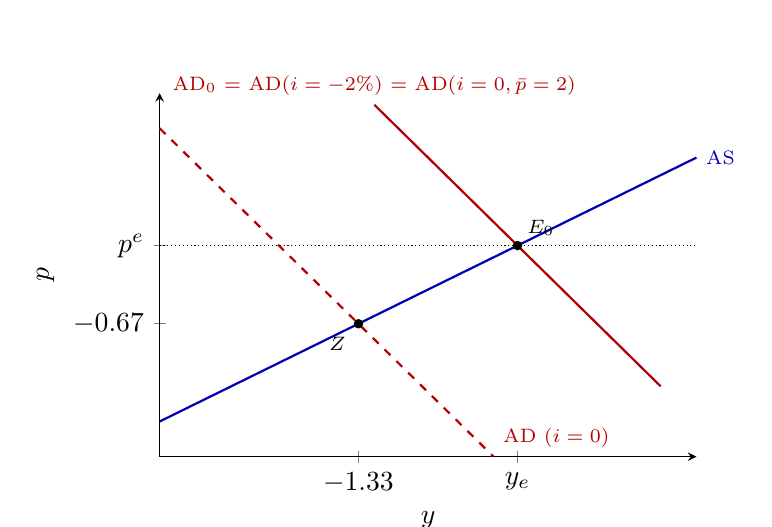
\begin{tikzpicture}
\begin{axis}[width=8.4cm,height=6.2cm,axis lines=left,xmin=-3,xmax=1.5,ymin=-1.8,ymax=1.3,clip=false,
  xlabel={$y$},ylabel={$p$},
  xtick={-1.3333,0},xticklabels={$-1.33$,$y_e$},ytick={-0.6667,0},yticklabels={$-0.67$,$p^e$}]
\addplot[densely dotted,domain=-3:1.5]{0};
\addplot[thick,blue!70!black,domain=-3:1.5]{0.5*x};
\addplot[thick,red!70!black,domain=-1.2:1.2]{-x};
\addplot[thick,red!70!black,dashed,domain=-3:-0.2]{-2-x};
\addplot[only marks,mark=*,mark size=1.5pt] coordinates {(0,0) (-1.3333,-0.6667)};
\node[font=\scriptsize,blue!70!black,anchor=west] at (axis cs:1.5,0.75) {AS};
\node[font=\scriptsize,red!70!black,anchor=south] at (axis cs:-1.2,1.2) {AD$_0$ $=$ AD($i=-2\%$) $=$ AD($i=0,\bar p=2$)};
\node[font=\scriptsize,red!70!black,anchor=south west] at (axis cs:-0.2,-1.8) {AD ($i=0$)};
\node[font=\scriptsize,anchor=north east] at (axis cs:-1.36,-0.70) {$Z$};
\node[font=\scriptsize,anchor=south west] at (axis cs:0,0) {$E_0$};
\end{axis}
\end{tikzpicture}\\
{\footnotesize The fall in $\bar y_n$ shifts AD left by 4; at $i=0$ it can only be brought back by 2, so the economy
sits at $Z$. Either $i=-2\%$ (infeasible) or $\bar p=2\%$ (a promise) puts AD back through $E_0$.}
\end{center}
\intuicao{Expecting to be poorer later, households cut consumption now. Only a negative real rate would persuade
them to spend; with $i$ stuck at zero, that negative real rate has to come from expected inflation.}
\refbib{Benigno (2015), \S9 (liquidity trap), Figs.~11--12, pp.~516--518; natural rate from \S5.}
\rubrica{
\item $r_n=-2\%$ derived and the desired $i$: 0.15. Calling it a supply shock or a trade-off: max.\ 0.2 on the item.
\item ZLB equilibrium $y=-1.33$, $p=-0.67$, gaps: 0.2 (slip: $-0.1$).
\item $\bar p=2\%$ and the real-rate mechanism, credibility: 0.2.
\item Graph: AS, AD shifted left, the partial return at $i=0$, point $Z$: 0.15.
}
\end{sol}

\parte{d}{0.9 point} Instead of a promise, the government raises current spending $g$ ($\bar g$ unchanged) while
$i$ stays at 0. Derive the multipliers $dy/dg$ and $d(y-y_e)/dg$, evaluate them, find the $g$ that closes the gap,
and check what happens to $p$. Then suppose the Copom were away from the ZLB and followed its optimal rule: what
would $dy/dg$ be? Explain why the ZLB makes fiscal policy more powerful here. Does Benigno's \S10 suggest even larger
multipliers? Show the effect of $g$ on the graph.
\resolespaco
\begin{sol}
\begin{notacao}
\item Symbols of (a)--(c) keep their meaning. New here:
\item $g\ge0$: current government spending, in percent of GDP; $\bar g=0$ unchanged.
\item $\omega\equiv\dfrac{\sigma^{-1}}{\sigma^{-1}+\eta}\in(0,1)$: response of $y_n$ and $y_e$ to $g$.
\item $dy/dg$: output multiplier. $d(y-y_e)/dg$: gap multiplier. $F$: the outcome with $g=4$.
\end{notacao}
\passo{1 --- $g$ moves both curves}{AD \eqref{q4:AD}: $+g$ one-for-one. AS: differentiate \eqref{q4:YN} and
\eqref{q4:YE} with respect to $g$:
\begin{equation}
\frac{dy_n}{dg}=\frac{dy_e}{dg}=\omega=\tfrac12, \label{q4d:omega}
\end{equation}
the wealth effect of taxes-to-come on labour supply. $y_n$ and $y_e$ rise by the same $\omega g$, so $g$ is not a
mark-up shock.}
\passo{2 --- solve}{Put $i=0$, $\bar p=0$, $\bar g=0$ in \eqref{q4:AD}:
\begin{align}
y &= \bar y_n+(g-0)-\sigma\big[(0)-(0-p)-\rho\big]\nonumber\\
&= \bar y_n+\sigma\rho+g-\sigma p. \label{q4d:ad}
\end{align}
AS \eqref{q4:AS} with $p^e=0$ and $y_n=\omega g$ from \eqref{q4d:omega}:
\begin{align}
p-(0) &= \kappa\big(y-(\omega g)\big)\nonumber\\
p &= \kappa(y-\omega g). \label{q4d:as}
\end{align}
Substitute \eqref{q4d:as} into \eqref{q4d:ad}:
\begin{align*}
y &= \bar y_n+\sigma\rho+g-\sigma\big(\kappa(y-\omega g)\big)\\
&= \bar y_n+\sigma\rho+g-\sigma\kappa y+\sigma\kappa\omega g\\
y(1+\sigma\kappa) &= \bar y_n+\sigma\rho+g(1+\sigma\kappa\omega).
\end{align*}
Differentiate with respect to $g$:
\begin{equation}
\boxed{\frac{dy}{dg}=\frac{1+\sigma\kappa\,\omega}{1+\sigma\kappa}}
=\frac{1+1\cdot\frac12\cdot\frac12}{1+1\cdot\frac12}=\boxed{\tfrac56}.
\label{q4d:mult}
\end{equation}
Subtract \eqref{q4d:omega} from \eqref{q4d:mult}:
\begin{align}
\frac{d(y-y_e)}{dg} &= \frac{1+\sigma\kappa\omega}{1+\sigma\kappa}-\omega\nonumber\\
&= \frac{1+\sigma\kappa\omega-\omega-\sigma\kappa\omega}{1+\sigma\kappa}\nonumber\\
&= \boxed{\frac{1-\omega}{1+\sigma\kappa}}=\frac{1-\frac12}{1+1\cdot\frac12}=\boxed{\tfrac13}. \label{q4d:gap}
\end{align}
These are Benigno's Table~1 $m_g=\frac{1}{1+\sigma\kappa}+\frac{\kappa}{(\sigma^{-1}+\eta)(1+\sigma\kappa)}$ and
$m_{\bar g}=\frac{\eta}{(\sigma^{-1}+\eta)(1+\sigma\kappa)}$ (with $\sigma\kappa\omega=\kappa/(\sigma^{-1}+\eta)$ and
$1-\omega=\eta/(\sigma^{-1}+\eta)$).}
\passo{3 --- closing the gap}{The gap at $Z$ is $-\tfrac43$ (part (c)). Divide by \eqref{q4d:gap}:
\[
g=\frac{4/3}{1/3}=\boxed{4\%}\ \text{of GDP}.
\]
Then, by \eqref{q4d:mult}, \eqref{q4d:omega} and \eqref{q4d:as}:
\begin{align*}
y &= -\tfrac43+\tfrac56\cdot4=\boxed{2},\\
y_n &= y_e=\omega g=\tfrac12\cdot4=2,\\
p &= \kappa(y-y_n)=\tfrac12(2-2)=\boxed{0=p^e}:
\end{align*}
both gaps closed, zero loss.}
\passo{4 --- away from the ZLB}{By \eqref{q4d:omega} spending moves $y_n$ and $y_e$ together, so there is no
trade-off: the optimal Copom satisfies \eqref{q4a:rule} with both gaps zero, $y=y_e(g)=\omega g$, $p=p^e$, raising
$i$ by $(1-\omega)g/\sigma$ to offset the excess demand in \eqref{q4:AD}. Then
$\boxed{dy/dg=\omega=\tfrac12}$.}
\passo{5 --- why larger at the ZLB}{Compare \eqref{q4d:mult} with $\omega$:
\[
\frac{1+\sigma\kappa\omega}{1+\sigma\kappa}>\omega\iff1>\omega\iff\eta>0.
\]
At the ZLB the Copom does not raise $i$ (it would like a \emph{lower} rate), so there is no crowding out through
the policy rate; only the price channel (a higher $p$ with $\bar p$ given raises the real rate) remains, which
keeps the multiplier below 1. In \S10 (Eggertsson--Krugman deleveraging) some households are
borrowing-constrained and spend every extra real of income, and falling prices raise real debt burdens: there the
multiplier at the ZLB can be much larger. With one representative household, as here, it stays at $5/6$.}
\begin{center}
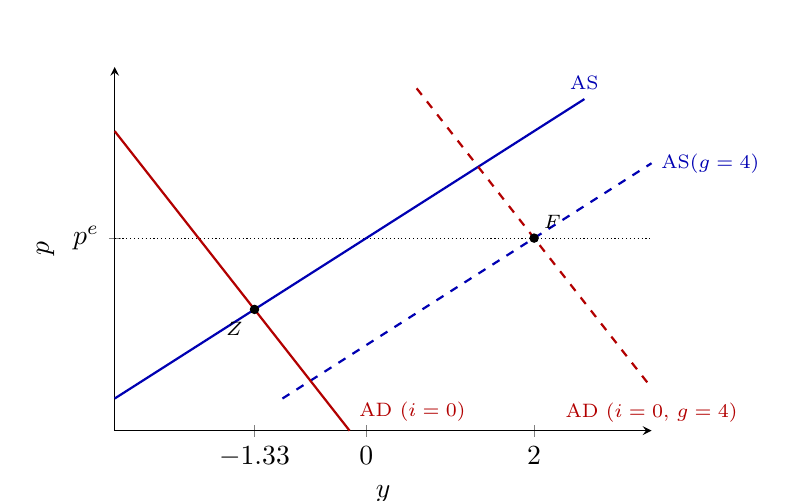
\begin{tikzpicture}
\begin{axis}[width=8.4cm,height=6.2cm,axis lines=left,xmin=-3,xmax=3.4,ymin=-1.8,ymax=1.6,clip=false,
  xlabel={$y$},ylabel={$p$},
  xtick={-1.3333,0,2},xticklabels={$-1.33$,$0$,$2$},ytick={0},yticklabels={$p^e$}]
\addplot[densely dotted,domain=-3:3.4]{0};
\addplot[thick,blue!70!black,domain=-3:2.6]{0.5*x};
\addplot[thick,blue!70!black,dashed,domain=-1:3.4]{0.5*(x-2)};
\addplot[thick,red!70!black,domain=-3:-0.2]{-2-x};
\addplot[thick,red!70!black,dashed,domain=0.6:3.4]{2-x};
\addplot[only marks,mark=*,mark size=1.5pt] coordinates {(-1.3333,-0.6667) (2,0)};
\node[font=\scriptsize,blue!70!black,anchor=south] at (axis cs:2.6,1.3) {AS};
\node[font=\scriptsize,blue!70!black,anchor=west] at (axis cs:3.4,0.7) {AS($g=4$)};
\node[font=\scriptsize,red!70!black,anchor=south west] at (axis cs:-0.2,-1.8) {AD ($i=0$)};
\node[font=\scriptsize,red!70!black,anchor=north] at (axis cs:3.4,-1.45) {AD ($i=0$, $g=4$)};
\node[font=\scriptsize,anchor=north east] at (axis cs:-1.36,-0.70) {$Z$};
\node[font=\scriptsize,anchor=south west] at (axis cs:2,0) {$F$};
\end{axis}
\end{tikzpicture}\\
{\footnotesize $g=4$ shifts AD right by 4 and AS right by $\omega g=2$; the new point $F=(2,\,p^e)$ has
$y=y_n=y_e$.}
\end{center}
\intuicao{Government spending adds demand directly and, by making households work more, adds supply too. When the
central bank is free it leans against the extra demand; stuck at zero it cannot, so more of the spending turns into
output.}
\refbib{Benigno (2015), \S8, eqs.~(22)--(23), Tables~1--2, pp.~514--516; \S9--\S10, pp.~516--521.}
\rubrica{
\item $g$ shifts AD and AS, with $\omega$: 0.15. Moving only AD: $-0.1$.
\item $dy/dg=5/6$ and $d(y-y_e)/dg=1/3$ derived: 0.25 (slip: $-0.1$). Reporting only the output multiplier: max.\ 0.15
on this line.
\item $g=4$ with $y=2$, $p=p^e$: 0.15.
\item Optimal-policy multiplier $\omega=1/2$ with the reason: 0.15.
\item Why larger at the ZLB and the \S10 remark: 0.1. Graph: 0.1.
}
\gap{Prova 01, Q3: which bar moves which curve, the sign of policy, and optimal policy as minimising the loss along AS;
here with a mark-up shock, where $\phi$ does matter, plus the ZLB and fiscal multipliers.}
\end{sol}

\ifsolucoes\else
\vfill
\begin{center}\footnotesize\textit{End of exam.}\end{center}
\fi

\end{document}
"   (run twice)
% Check fonts: pdffonts <file>.pdf  (all Type 1).
% Every number and closed form in the key: python simulado_codigo/check_simulado_05.py
% =============================================================================
\documentclass[11pt,a4paper]{article}
\usepackage[utf8]{inputenc}
\usepackage[T1]{fontenc}
\usepackage{lmodern}   % Type 1 vector fonts (replaces PK bitmaps)
\usepackage{cmap}      % ToUnicode CMap -> copyable text and accents
\usepackage[english]{babel}
\usepackage{amsmath,amssymb,amsfonts}
\usepackage[a4paper,margin=2.2cm]{geometry}
\usepackage{enumitem}
\usepackage{fancyhdr}
\usepackage{comment}
\usepackage{xcolor}
\usepackage{microtype}
\usepackage{booktabs}
\usepackage{needspace}
\usepackage{pgfplots}
\pgfplotsset{compat=1.18}
\usetikzlibrary{arrows.meta}

% ====================== CONFIGURATION ======================
\newif\ifsolucoes
\ifdefined\withsolutions\solucoestrue\else\solucoesfalse\fi

\newcommand{\disciplina}{Macroeconomics I --- MPE Insper}
\newcommand{\listatema}{Mock Exam 5}
\newcommand{\espacoresol}{6cm}

% ====================== MACHINERY ======================
\def\DefaultCutFileName{\def\CommentCutFile{\jobname.cut}}  % per-job cut file: parallel builds in Simulados/ would share comment.cut
\ifsolucoes\includecomment{sol}\else\excludecomment{sol}\fi

\pagestyle{fancy}\fancyhf{}
\lhead{\footnotesize\disciplina}
\rhead{\footnotesize \listatema\ifsolucoes{} --- Solutions and Rubric\fi}
\cfoot{\footnotesize\thepage}
\renewcommand{\headrulewidth}{0.3pt}
\setlength{\headheight}{14pt}

\setlist{topsep=2pt,itemsep=2pt}
\newcounter{questao}

\newcommand{\questao}[1]{\Needspace{12\baselineskip}\refstepcounter{questao}\bigskip\noindent
  {\large\bfseries\color{blue!55!black}Question \thequestao.}~#1\par\smallskip}
\newcommand{\parte}[2]{\par\Needspace{6\baselineskip}\medskip\noindent\textbf{#1)}~(#2)~}
\newcommand{\resolespaco}{\ifsolucoes\else\par\textit{Solution:}\vspace{\espacoresol}\par\fi}
\newcommand{\passo}[2]{\par\smallskip\noindent\textbf{Step #1.}~#2}
\newcommand{\intuicao}[1]{\par\smallskip\noindent\textit{Intuition.}~#1}
\newcommand{\refbib}[1]{\par\smallskip\noindent{\footnotesize\color{black!60}\textbf{Ref:} #1}}
\newcommand{\gap}[1]{\par\smallskip\noindent{\footnotesize\color{red!55!black}\textbf{Gap targeted:} #1}}
\newcommand{\trap}[1]{\par\smallskip\noindent{\small\color{red!55!black}\#~#1}}
\newcommand{\rubrica}[1]{\par\needspace{4\baselineskip}\smallskip\noindent\textbf{Grading rubric.}\begin{itemize}[leftmargin=1.4em,topsep=1pt]#1\end{itemize}}
\newenvironment{notacao}{\par\smallskip\noindent\textbf{Notation.}\begin{itemize}[leftmargin=1.4em,topsep=1pt,itemsep=0pt]\small}{\end{itemize}}
\allowdisplaybreaks
% Equation numbering: statement equations carry letter tags, (S1)-(S2), (U), (F), (BC), (AD), (AS), (YN),
% (YE), (LF), identical in both builds; solution equations are numbered (1), (2), ... and exist only in the
% solutions build. Labels are prefixed by item (q2b:...); statement text never cites a solution label.

% =============================================================================
\begin{document}
\begin{center}
  {\Large\bfseries \disciplina}\\[2pt]
  {\large \listatema\ (Simulado 5) --- whole course --- 2026, 3rd term}\ifsolucoes\\[2pt]\textit{Solutions and Grading Rubric}\fi
\end{center}
\vspace{2pt}

{\footnotesize\noindent\textbf{Instructions.} Four questions, 10 points in total. Duration: 3 hours, closed
book, non-programmable calculator allowed. Show every step; box final answers; sign every derivative before
interpreting it; in diagrams label the axes, name every curve and mark the direction of every shift.
Notation: Kurlat (2020) in Questions 1--3, Benigno (2015) in Question 4. All numbers are illustrative.
Natural logarithms throughout.\par}

\ifsolucoes
\medskip
{\footnotesize\noindent\textbf{How the rubric works.} Conceptual caps (``max.\ $x$'') bound an item whatever
else is right. Light penalties ($-0.1$) apply to arithmetic slips with a correct method. Caps and penalties
are \emph{not cumulative}: when a cap applies, the penalties inside it are ignored. Each question ends with the
weak spot it retests (``Gap targeted''). Every number and closed form below is recomputed by
\texttt{simulado\_codigo/check\_simulado\_05.py}.\par}
\fi

% =============================================================================
\questao{(2.0 points) Coffee, schools and saving in Minas Gerais.}

\noindent\textbf{Part A --- measurement.} One year in a coffee region, values in R\$ million.
\begin{itemize}[leftmargin=1.4em]
\item A trading company imports fertiliser for 50 and sells all of it to a coffee farm for 80. It pays 10 in wages.
\item The farm harvests coffee worth 300 at market prices. It sells 200 to a roaster, exports 60 to Germany, and
the remaining 40 is still in its warehouse, unsold, at the end of the year. It pays 120 in wages.
\item The roaster also imports packaging for 20 and sells all its roasted coffee, 450, to Brazilian households.
It pays 150 in wages.
\item The state government runs free public schools: it pays teachers 100 and buys nothing else.
\end{itemize}
Each firm's profit is whatever remains of its revenue after inputs and wages.

\parte{a}{1.0 point} (i) Compute the region's GDP by the product (value-added), income and expenditure
approaches, and show that they agree. (ii) Next year the farm harvests nothing. It sells its 40 of stored coffee
to the roaster, which roasts it and sells it to households for 90; nothing else happens in this chain. Compute
the chain's contribution to next year's GDP by the product and the expenditure approaches. (iii) A columnist
writes: ``This year's GDP overstates the region's output, because 40 of coffee was never sold; and it understates
it, because the schools charge nothing.'' Evaluate each half of the claim.
\resolespaco
\begin{sol}
\begin{notacao}
\item Trader, farm, roaster, government: the four producers; $j$ indexes them. All values in R\$ million.
\item $VA_j\ge0$: value added of producer $j$, its gross output minus the intermediate inputs it uses up
(imported inputs included).
\item $\text{wages}_j\ge0$, $\text{profit}_j$: payments to workers and the operating surplus left to owners.
\item $C$, $I$, $G$, $X$, $M$: household consumption, investment (fixed capital plus change in inventories,
so $I$ can be negative), government purchases, exports and imports, all $\ge0$ except $I$.
\end{notacao}
\passo{0 --- the definitions used below}{GDP is the market value of final goods and services produced in the
region in the year. The three approaches:
\begin{align}
VA_j &= \text{gross output}_j-\text{intermediate inputs}_j, \label{q1a:va}\\
\text{GDP} &= \textstyle\sum_j VA_j, \label{q1a:prod}\\
\text{profit}_j &= VA_j-\text{wages}_j, \label{q1a:profit}\\
\text{GDP} &= \textstyle\sum_j(\text{wages}_j+\text{profit}_j), \label{q1a:inc}\\
\text{GDP} &= C+I+G+X-M. \label{q1a:exp}
\end{align}
Non-market output (public schools) has no price, so its gross output is valued \emph{at cost}.}
\passo{1 --- value added (product)}{Apply \eqref{q1a:va} to each producer. The farm's output is the whole
harvest, sold or not; the government's is its cost:
\begin{align*}
VA_{\text{trader}} &= 80-50=30,\\
VA_{\text{farm}} &= 300-80=220,\\
VA_{\text{roaster}} &= 450-200-20=230,\\
VA_{\text{gov}} &= 100.
\end{align*}
Sum with \eqref{q1a:prod}:
\[
\text{GDP}=30+220+230+100=\boxed{580}.
\]}
\passo{2 --- income}{Wages paid by the four producers:
\[
10+120+150+100=380.
\]
Profits from \eqref{q1a:profit}, using the value added of Step 1:
\begin{align*}
\text{profit}_{\text{trader}} &= 30-10=20,\\
\text{profit}_{\text{farm}} &= 220-120=100\quad\text{(it includes the 40 of stock, at market price)},\\
\text{profit}_{\text{roaster}} &= 230-150=80,\\
\text{profit}_{\text{gov}} &= 100-100=0\quad\text{(valued at cost, so no surplus)}.
\end{align*}
Sum with \eqref{q1a:inc}:
\[
\text{GDP}=380+20+100+80=\boxed{580}.
\]}
\passo{3 --- expenditure}{Final uses: households buy the roasted coffee, $C=450$; the unsold coffee is output
kept by its producer, \emph{inventory investment} $I=40$; $G=100$; $X=60$. Imports:
\[
M=50+20=70.
\]
Substitute into \eqref{q1a:exp}:
\[
\text{GDP}=450+40+100+60-70=\boxed{580}.
\]}
\begin{center}\small
\begin{tabular}{@{}lccccc@{}}
\toprule
Approach & Trader & Farm & Roaster & Government & GDP\\
\midrule
Product (VA) & 30 & 220 & 230 & 100 & \textbf{580}\\
Income (wages $+$ profit) & $10+20$ & $120+100$ & $150+80$ & $100+0$ & \textbf{580}\\
Expenditure & \multicolumn{4}{c}{$C=450,\ I=40,\ G=100,\ X=60,\ M=-70$} & \textbf{580}\\
\bottomrule
\end{tabular}
\end{center}
\passo{4 --- next year}{Product, by \eqref{q1a:va}: the farm produces nothing new (selling an old stock is not
production), so $VA_{\text{farm}}=0$, and
\[
VA_{\text{roaster}}=90-40=\boxed{50}.
\]
Expenditure, by \eqref{q1a:exp}: $C=+90$, and inventories fall, $I=-40$:
\[
\text{GDP}_{\text{chain}}=90-40=\boxed{50}.
\]
The 40 was counted last year as investment; counting it again as consumption would double-count it, so the
inventory drawdown enters as \emph{negative} investment.}
\passo{5 --- the columnist}{First half: \textbf{wrong}. GDP measures production, not sales; the 40 was
produced this year and \eqref{q1a:exp} records it as investment in inventories. Second half:
\textbf{wrong as stated}. The schools are in GDP, valued at the cost of the teachers (100), even with a zero
price. What GDP may miss is any value of the service above its cost --- a ``beyond GDP'' issue, not an omission.
Contrast with Prova 01: a free online service paid by advertising enters only through the ad revenue, which is
an intermediate input of the advertiser.}
\intuicao{Every real a firm earns is either a payment to a factor or a purchase from another firm; summing value
added nets out the purchases. Imports are subtracted because they are someone else's production; stocks are
added because they are this year's production that nobody bought yet.}
\refbib{Kurlat ch.~1, \S1.1, pp.~15--21: inventories p.~18; government output at cost, Example~1.7, p.~20.}
\rubrica{
\item (i) Each approach with its own entries: 0.2 each (0.6). Treating the 40 as not produced, or leaving
imports in VA: max.\ 0.3 on (i). Putting the teachers into $C$ instead of $G$: $-0.1$.
\item (ii) 50 by both approaches, with $I=-40$: 0.2. Adding the 40 again (GDP 90): 0 on (ii).
\item (iii) Both halves, each with its reason: 0.2.
}
\end{sol}

\medskip
\noindent\textbf{Part B --- saving and growth.} The Ministry of Planning uses the Solow model in
\emph{per-worker} terms, with no technological progress, saving rate $s$, population growth $n$
and depreciation $\delta$ constant:
\begin{align}
y &= Ak^{\alpha}, \tag{S1}\label{q1:prod}\\
(1+n)k_{t+1} &= (1-\delta)k_t+sAk_t^{\alpha}. \tag{S2}\label{q1:lom}
\end{align}
Brazil is in steady state with $\alpha=1/3$ and $s=0.15$.

\parte{b}{1.0 point} (i) Derive steady-state capital $k^{*}$ and consumption $c^{*}$ per worker as functions of
$s$, and find the saving rate $s_{GR}$ that maximises $c^{*}$. Confirm it with a condition on the marginal
product of capital. (ii) A pension reform raises the saving rate permanently from $0.15$ to $s_{GR}$ at date
$t_0$. Compute the percentage change in consumption per worker on impact and between the two steady states,
and the change in steady-state output per worker. (iii) Show graphically: the Solow diagram before and after
the reform, and the time paths of $y$ and $c$. (iv) Is the reform necessarily good for Brazilians? Who pays for
it?
\resolespaco
\begin{sol}
\begin{notacao}
\item $y_t$, $k_t$, $c_t>0$: output, capital and consumption per worker at date $t$.
\item $A>0$: total factor productivity, constant. $\alpha\in(0,1)$: capital's income share ($\alpha=1/3$).
\item $s\in(0,1)$: saving rate. $n\ge0$: population growth. $\delta\in(0,1)$: depreciation rate.
\item $k^*$, $y^*$, $c^*$: steady-state values. $s_{GR}$: the golden-rule saving rate.
\item $t_0$: date of the reform; ``old'' and ``new'' index the steady states at $s=0.15$ and $s=s_{GR}$.
\end{notacao}
\passo{1 --- steady state}{Set $k_{t+1}=k_t=k^*$ in \eqref{q1:lom}:
\begin{align}
(1+n)k^* &= (1-\delta)k^*+sA(k^*)^{\alpha}\nonumber\\
(n+\delta)k^* &= sA(k^*)^{\alpha}\nonumber\\
(k^*)^{1-\alpha} &= \frac{sA}{n+\delta}. \nonumber
\end{align}
Raise both sides to the power $1/(1-\alpha)$:
\begin{equation}
\boxed{k^*=\left(\frac{sA}{n+\delta}\right)^{\frac{1}{1-\alpha}}} \label{q1b:kss}
\end{equation}
Consumption is the part of output not saved:
\begin{equation}
c=(1-s)\,y. \label{q1b:c}
\end{equation}
Evaluate \eqref{q1:prod} at \eqref{q1b:kss}:
\begin{align}
y^* &= A(k^*)^{\alpha}\nonumber\\
&= A\left[\left(\frac{sA}{n+\delta}\right)^{\frac{1}{1-\alpha}}\right]^{\alpha}\nonumber\\
&= A\left(\frac{sA}{n+\delta}\right)^{\frac{\alpha}{1-\alpha}}. \label{q1b:yss}
\end{align}
Substitute \eqref{q1b:yss} into \eqref{q1b:c}:
\begin{align}
c^* &= (1-s)\left[A\left(\frac{sA}{n+\delta}\right)^{\frac{\alpha}{1-\alpha}}\right]\nonumber\\
&= \boxed{(1-s)A\left(\frac{sA}{n+\delta}\right)^{\frac{\alpha}{1-\alpha}}} \label{q1b:css}
\end{align}
\#~The exponent is $\alpha/(1-\alpha)$: $k^*$ is raised to $\alpha$ inside $f$.}
\passo{2 --- golden rule}{Take the log of \eqref{q1b:css}:
\begin{equation}
\ln c^*=\ln A+\ln(1-s)+\frac{\alpha}{1-\alpha}\Big[\ln s+\ln A-\ln(n+\delta)\Big]. \label{q1b:lnc}
\end{equation}
Differentiate \eqref{q1b:lnc} with respect to $s$ and set it to zero:
\begin{equation}
-\frac{1}{1-s}+\frac{\alpha}{(1-\alpha)s}=0. \label{q1b:foc}
\end{equation}
Multiply \eqref{q1b:foc} by $(1-\alpha)s(1-s)>0$:
\begin{align*}
-(1-\alpha)s+\alpha(1-s) &= 0\\
\alpha-s &= 0.
\end{align*}
Hence
\begin{equation}
\boxed{s_{GR}=\alpha=\tfrac13}. \label{q1b:sgr}
\end{equation}
SOC: differentiating \eqref{q1b:foc} again gives $-\frac{1}{(1-s)^2}-\frac{\alpha}{(1-\alpha)s^2}<0$, a maximum.}
\passo{2b --- cross-check through $k$}{In a steady state, \eqref{q1:lom} with $k_{t+1}=k_t=k$ gives
\begin{equation}
sAk^{\alpha}=(n+\delta)\,k. \label{q1b:ss}
\end{equation}
Substitute \eqref{q1:prod} into \eqref{q1b:c}, then use \eqref{q1b:ss}:
\begin{align}
c &= (1-s)\big(Ak^{\alpha}\big)\nonumber\\
&= Ak^{\alpha}-sAk^{\alpha}\nonumber\\
&= Ak^{\alpha}-\big((n+\delta)k\big)\nonumber\\
&= Ak^{\alpha}-(n+\delta)k. \label{q1b:ck}
\end{align}
Set the derivative of \eqref{q1b:ck} with respect to $k$ to zero:
\begin{equation}
\boxed{\alpha Ak^{\alpha-1}=n+\delta}\qquad(\text{MPK}=n+\delta). \label{q1b:mpk}
\end{equation}
Solve \eqref{q1b:ss} for $s$ and substitute \eqref{q1b:mpk} for $n+\delta$:
\begin{align*}
s &= \frac{(n+\delta)k}{Ak^{\alpha}}\\
&= \frac{\big(\alpha Ak^{\alpha-1}\big)\,k}{Ak^{\alpha}}\\
&= \alpha\ \checkmark
\end{align*}
Knife edge: $\alpha\to0\Rightarrow s_{GR}\to0$ (capital useless, save nothing). The Prova~01 slip (exponent
$1/(1-\alpha)$ instead of $\alpha/(1-\alpha)$) gives $s=1/(2-\alpha)=0.6$ here, which fails this test.}
\passo{3 --- impact}{At $t_0$ capital is predetermined, so $y$ does not move and, by \eqref{q1b:c}, only the
factor $1-s$ changes:
\begin{align*}
\frac{c_{t_0}}{c_{\text{old}}} &= \frac{(1-s_{GR})\,y^*_{\text{old}}}{(1-0.15)\,y^*_{\text{old}}}\\
&= \frac{1-1/3}{1-0.15}\\
&= \frac{0.6667}{0.85}\\
&= 0.7843,
\end{align*}
a fall of $\boxed{21.6\%}$.}
\passo{4 --- long run}{Divide \eqref{q1b:css} at $s_{GR}$ by \eqref{q1b:css} at $0.15$; $A$, $n$ and $\delta$ cancel,
and $(1/3)/0.15=2.2222$, $\alpha/(1-\alpha)=1/2$:
\begin{align*}
\frac{c^*_{\text{new}}}{c^*_{\text{old}}} &= \frac{(1-1/3)A\left(\frac{(1/3)A}{n+\delta}\right)^{\frac{1/3}{2/3}}}
{(1-0.15)A\left(\frac{0.15A}{n+\delta}\right)^{\frac{1/3}{2/3}}}\\
&= \frac{1-1/3}{1-0.15}\left(\frac{1/3}{0.15}\right)^{\frac{1/3}{2/3}}\\
&= 0.7843\times(2.2222)^{1/2}\\
&= 0.7843\times1.4907\\
&= 1.1692,
\end{align*}
a rise of $\boxed{16.9\%}$. Output, from the ratio of \eqref{q1b:yss}:
\begin{align*}
\frac{y^*_{\text{new}}}{y^*_{\text{old}}} &= \frac{A\left(\frac{(1/3)A}{n+\delta}\right)^{1/2}}{A\left(\frac{0.15A}{n+\delta}\right)^{1/2}}\\
&= (2.2222)^{1/2}=1.4907,\quad\boxed{+49.1\%}.
\end{align*}
Capital, from the ratio of \eqref{q1b:kss} (exponent $1/(1-\alpha)=3/2$): $(2.2222)^{3/2}=3.313$.}
\passo{5 --- graphs}{Left: $sAk^{\alpha}$ rotates up, and the crossing with $(n+\delta)k$, \eqref{q1b:ss}, moves
from $k^*_{\text{old}}$ to $k^*_{GR}$; arrows along the $k$ axis point right in between. Right: $y$ starts at its
old level and rises monotonically (no jump, $k$ is a stock); $c$ jumps down at $t_0$, then rises, overtakes its
old level and converges to a level 16.9\% higher. The curves are simulated from \eqref{q1:lom} with $A=1$,
$n=1\%$, $\delta=5\%$ a year; with these values $c$ regains its old level after 18 years.}
\begin{center}
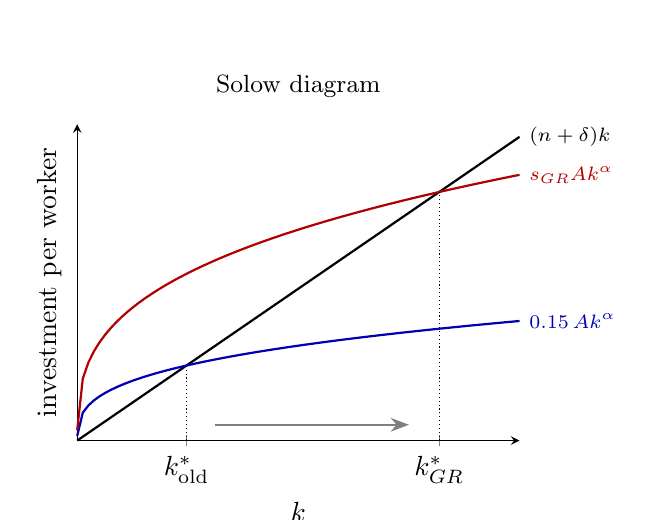
\begin{tikzpicture}
\begin{axis}[width=7.2cm,height=5.6cm,axis lines=left,xmin=0,xmax=16,ymin=0,ymax=1.0,
  xlabel={$k$},ylabel={investment per worker},xtick={3.953,13.095},xticklabels={$k^*_{\text{old}}$,$k^*_{GR}$},
  ytick=\empty,title={\small Solow diagram},clip=false]
\addplot[thick,black,domain=0:16,samples=60]{0.06*x};
\addplot[thick,blue!70!black,domain=0.001:16,samples=80]{0.15*x^(1/3)};
\addplot[thick,red!70!black,domain=0.001:16,samples=80]{(1/3)*x^(1/3)};
\addplot[densely dotted] coordinates {(3.953,0) (3.953,0.2372)};
\addplot[densely dotted] coordinates {(13.095,0) (13.095,0.7857)};
\node[font=\scriptsize,anchor=west] at (axis cs:16,0.96) {$(n+\delta)k$};
\node[font=\scriptsize,blue!70!black,anchor=west] at (axis cs:16,0.378) {$0.15\,Ak^{\alpha}$};
\node[font=\scriptsize,red!70!black,anchor=west] at (axis cs:16,0.84) {$s_{GR}Ak^{\alpha}$};
\draw[-{Stealth},thick,gray] (axis cs:5,0.05)--(axis cs:12,0.05);
\end{axis}
\end{tikzpicture}\quad
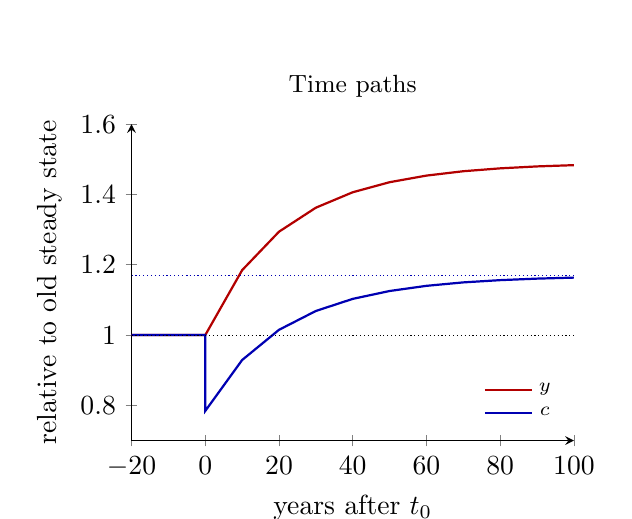
\begin{tikzpicture}
\begin{axis}[width=7.2cm,height=5.6cm,axis lines=left,xmin=-20,xmax=100,ymin=0.7,ymax=1.6,
  xlabel={years after $t_0$},ylabel={relative to old steady state},title={\small Time paths},
  legend style={font=\scriptsize,draw=none,at={(0.98,0.03)},anchor=south east}]
\addplot[thick,red!70!black] coordinates {(-20,1) (0,1) (10,1.1847) (20,1.2941) (30,1.3624) (40,1.4063)
  (50,1.4349) (60,1.4537) (70,1.4661) (80,1.4743) (90,1.4798) (100,1.4834)};
\addplot[thick,blue!70!black] coordinates {(-20,1) (0,1) (0,0.7843) (10,0.9291) (20,1.0150) (30,1.0686)
  (40,1.1030) (50,1.1254) (60,1.1401) (70,1.1499) (80,1.1563) (90,1.1606) (100,1.1635)};
\addplot[densely dotted,domain=-20:100]{1};
\addplot[densely dotted,blue!70!black,domain=-20:100]{1.1692};
\legend{$y$,$c$}
\end{axis}
\end{tikzpicture}
\end{center}
\passo{6 --- welfare}{Not necessarily. Brazil starts \emph{below} the golden rule ($0.15<1/3$), so the economy
is dynamically efficient and more steady-state consumption must be bought with less consumption during the
transition: current workers and retirees pay (21.6\% less consumption at once, below the old level for 18
years); later cohorts gain. Whether it is worth it depends on how the future is discounted --- an impatient
society optimally stays below $s_{GR}$ (compare optimal and fixed saving rates, Kurlat ex.~9.12, p.~185).
Only from \emph{above} $s_{GR}$ would a change (a cut in $s$) raise consumption at every date, a Pareto
improvement.}
\intuicao{A higher saving rate keeps raising output, but each extra unit of capital also needs $n+\delta$ of
replacement; past the point where MPK $=n+\delta$, capital costs more to maintain than it adds. With
Cobb--Douglas that point is reached exactly when the saving rate equals capital's income share.}
\refbib{Kurlat ch.~4, \S4.2 (steady state, pp.~59--61) and \S4.3 (golden rule, pp.~61--63); Jones (2020) ch.~5
for the transition paths.}
\rubrica{
\item (i) $k^*$ and $c^*$ with the exponent $\alpha/(1-\alpha)$: 0.15; $s_{GR}=\alpha$ derived: 0.1; MPK
cross-check: 0.1. Dropping the exponent (answer other than $\alpha$): max.\ 0.15 on (i). Maximising $k^*$ or
$y^*$ instead of $c^*$: 0 on (i).
\item (ii) Impact $-21.6\%$ with the reason (predetermined $k$): 0.1; $+16.9\%$ and $+49.1\%$: 0.15 (slip:
$-0.1$). Consumption rising on impact: 0 on that line.
\item (iii) Solow diagram with both curves and both crossings labelled: 0.1; time paths, $c$ jumping down and
$y$ not jumping: 0.1.
\item (iv) Trade-off and who pays: 0.1; why only above $s_{GR}$ is a change Pareto improving: 0.1.
}
\gap{Prova 01, 1.b--1.c (three approaches with all entries; what counts as investment) and 2.b (golden-rule
algebra: carry the exponent, cross-check with MPK $=n+\delta$).}
\end{sol}

% =============================================================================
\questao{(2.5 points) A labour tax: what it does depends on what the government does with the money.
\textnormal{\normalsize A one-period economy has a fixed capital stock $\bar K$, owned by the representative
household, which also owns the competitive firm. The household has one unit of time and utility
\eqref{q2:U}, with $\psi=1/3$. The firm produces \eqref{q2:F} with $\alpha=1/3$;
normalise $A\bar K^{\alpha}=1$. Labour income is taxed at rate $\tau$, so the household's budget is
\eqref{q2:BC}, where $T$ is a lump-sum transfer that the household takes as given:
\begin{align}
u &= \ln c+\psi\ln(1-L), \tag{U}\label{q2:U}\\
Y &= A\bar K^{\alpha}L^{1-\alpha}, \tag{F}\label{q2:F}\\
c &= (1-\tau)wL+r\bar K+\Pi+T. \tag{BC}\label{q2:BC}
\end{align}
Congress debates a 25\% tax on labour income.}}

\parte{a}{0.7 point} Let $\tau=T=0$. Write the household's and the firm's problems, their first-order
conditions and the market-clearing conditions; show that profits are zero, and find the equilibrium $L$, $Y$,
$w$ and $c$. Then solve the problem of a planner who chooses $c$ and $L$ subject only to technology, and show that
it gives the same allocation. State the theorem behind this and the assumptions it needs.
\resolespaco
\begin{sol}
\begin{notacao}
\item $c\ge0$: consumption. $L\in[0,1]$: hours worked; $1-L$: leisure (one unit of time).
\item $\psi>0$: weight of leisure in utility ($\psi=1/3$).
\item $Y$: output. $\bar K>0$: fixed capital stock. $A>0$: productivity, with $A\bar K^{\alpha}=1$.
$\alpha\in(0,1)$: capital's share ($\alpha=1/3$).
\item $w$, $r>0$: real wage and real rental rate of capital. $\Pi$: the firm's profit, paid to the household.
\item $\tau\in[0,1)$: tax rate on labour income. $T$: lump-sum transfer. In this item $\tau=T=0$.
\item $L_0$, $Y_0$, $w_0$, $c_0$: the equilibrium at $\tau=0$. $L^{P}$: the planner's choice.
\item MRS: marginal rate of substitution of leisure for consumption. MPL: marginal product of labour.
\end{notacao}
\passo{1 --- household}{With $\tau=T=0$, \eqref{q2:BC} is
\begin{equation}
c=wL+r\bar K+\Pi. \label{q2a:bc}
\end{equation}
Substitute \eqref{q2a:bc} into \eqref{q2:U}:
\[
\max_L\ \ln(wL+r\bar K+\Pi)+\psi\ln(1-L).
\]
Differentiate with respect to $L$ and set it to zero:
\[
\frac{w}{c}-\frac{\psi}{1-L}=0.
\]
Rearrange:
\begin{equation}
\boxed{\frac{\psi c}{1-L}=w} \label{q2a:hh}
\end{equation}
--- the marginal rate of substitution between leisure and consumption equals the real wage, the price of
leisure.}
\passo{2 --- firm}{The firm chooses $L$ and rents $\bar K$:
$\max\ A\bar K^{\alpha}L^{1-\alpha}-wL-r\bar K$. Differentiating \eqref{q2:F}:
\begin{align}
w &= (1-\alpha)A\bar K^{\alpha}L^{-\alpha}\nonumber\\
&= \frac{(1-\alpha)\big(A\bar K^{\alpha}L^{1-\alpha}\big)}{L}\nonumber\\
&= \frac{(1-\alpha)Y}{L}, \label{q2a:w}\\
r &= \alpha A\bar K^{\alpha-1}L^{1-\alpha}\nonumber\\
&= \frac{\alpha\big(A\bar K^{\alpha}L^{1-\alpha}\big)}{\bar K}\nonumber\\
&= \frac{\alpha Y}{\bar K}. \label{q2a:r}
\end{align}
Profits, using \eqref{q2a:w} and \eqref{q2a:r}:
\begin{align}
\Pi &= Y-wL-r\bar K\nonumber\\
&= Y-\left(\frac{(1-\alpha)Y}{L}\right)L-\left(\frac{\alpha Y}{\bar K}\right)\bar K\nonumber\\
&= Y-(1-\alpha)Y-\alpha Y\nonumber\\
&= \boxed{0} \label{q2a:pi}
\end{align}
(constant returns: factor payments exhaust output).}
\passo{3 --- clearing}{Labour: household supply $=$ firm demand; capital: $\bar K$; goods (no $G$):
\begin{equation}
c=Y. \label{q2a:goods}
\end{equation}}
\passo{4 --- solve}{Substitute \eqref{q2a:goods} and \eqref{q2a:w} into \eqref{q2a:hh}:
\begin{align*}
\frac{\psi\,(Y)}{1-L} &= \left(\frac{(1-\alpha)Y}{L}\right)\\
\psi L &= (1-\alpha)(1-L)\\
(1-\alpha+\psi)L &= 1-\alpha.
\end{align*}
Hence
\begin{align}
L_0 &= \boxed{\frac{1-\alpha}{1-\alpha+\psi}}\nonumber\\
&= \frac{1-\frac13}{1-\frac13+\frac13}\nonumber\\
&= \frac{2/3}{1}=\boxed{\tfrac23}. \label{q2a:L0}
\end{align}
Then, by \eqref{q2:F} with $A\bar K^{\alpha}=1$, \eqref{q2a:w}, \eqref{q2a:goods} and \eqref{q2a:r}:
\begin{align*}
Y_0 &= (2/3)^{2/3}=0.7631,\\
w_0 &= \frac{(2/3)(0.7631)}{2/3}=0.7631,\\
c_0 &= Y_0=0.7631,\\
r\bar K &= \alpha Y_0=\tfrac13(0.7631)=0.2544.
\end{align*}}
\passo{5 --- planner}{The planner substitutes technology \eqref{q2:F} into \eqref{q2:U}:
\begin{align}
\max_L\ \ln\!\big(A\bar K^{\alpha}L^{1-\alpha}\big)+\psi\ln(1-L)
=\text{const}+(1-\alpha)\ln L+\psi\ln(1-L). \label{q2a:plan}
\end{align}
Differentiate \eqref{q2a:plan} with respect to $L$:
\begin{equation}
\frac{1-\alpha}{L}=\frac{\psi}{1-L}. \label{q2a:planfoc}
\end{equation}
Cross-multiplying \eqref{q2a:planfoc} gives the second line of Step 4, so $L^{P}=\tfrac23$ (SOC: both terms
concave). The planner sets MRS $=$ MPL; the market sets MRS $=w$ \eqref{q2a:hh} and MPL $=w$ \eqref{q2a:w},
hence MRS $=$ MPL.}
\passo{6 --- theorem}{\textbf{First Welfare Theorem}: a competitive equilibrium is Pareto efficient, given
price-taking agents, complete markets, no externalities and no distortionary taxes. Here all hold at $\tau=0$.}
\refbib{Kurlat ch.~9, \S9.1--\S9.2, pp.~165--172 (equilibrium and the First Welfare Theorem); ch.~7, \S7.2,
pp.~131--137 (consumption--leisure choice).}
\rubrica{
\item Household FOC (MRS $=w$) and firm FOCs: 0.2. $\Pi=0$ shown: 0.1. Clearing conditions listed: 0.1.
\item $L_0=2/3$ with $Y,w,c$: 0.1 (slip: $-0.1$).
\item Planner's FOC and same allocation: 0.1. Theorem and its assumptions: 0.1.
\item Omitting capital income or profits from the budget: max.\ 0.4 on the item.
}
\end{sol}

\parte{b}{0.7 point} Now $\tau=25\%$ and the government returns the whole revenue as the transfer, so
$T=\tau wL$ in equilibrium. Find $L$ (in general and in numbers). Explain why returning the money does not undo
the effect of the tax. Show graphically, in the plane (leisure $\ell=1-L$, consumption $c$): the production
possibilities frontier, the equilibrium of (a), the new equilibrium, and the household's budget line at the new
equilibrium, with and without the transfer. Use the graph to explain why the new allocation is inefficient.
\resolespaco
\begin{sol}
\begin{notacao}
\item Symbols of (a) keep their meaning. New here:
\item $\tau=0.25$; $T=\tau wL$: the rebate, equal to the revenue in equilibrium, taken as given by the household.
\item $L_R$: hours under the rebated tax. $\ell\equiv1-L\in[0,1]$: leisure; $\ell_0$, $\ell_R$ at the two equilibria.
\item $E_0$, $E_R$: the equilibria of (a) and (b). $U_0$, $U_R$: the indifference curves through them.
\end{notacao}
\passo{1 --- FOC with the tax}{Substitute \eqref{q2:BC} into \eqref{q2:U}:
\[
\max_L\ \ln\big((1-\tau)wL+r\bar K+\Pi+T\big)+\psi\ln(1-L).
\]
Differentiate with respect to $L$, with $T$ taken as given, and set it to zero:
\[
\frac{(1-\tau)w}{c}-\frac{\psi}{1-L}=0.
\]
Rearrange, as in (a), now with $(1-\tau)w$ per hour:
\begin{equation}
\boxed{\frac{\psi c}{1-L}=(1-\tau)w}. \label{q2b:hh}
\end{equation}
$T$ does not appear: the household takes it as given, so it moves income, not the price of leisure.}
\passo{2 --- equilibrium}{The government returns the revenue:
\begin{equation}
T=\tau wL. \label{q2b:gov}
\end{equation}
Substitute \eqref{q2b:gov} into \eqref{q2:BC}, with $\Pi=0$ from \eqref{q2a:pi}, and then use \eqref{q2a:w} and
\eqref{q2a:r}:
\begin{align}
c &= (1-\tau)wL+r\bar K+(0)+(\tau wL)\nonumber\\
&= wL+r\bar K\nonumber\\
&= \left(\frac{(1-\alpha)Y}{L}\right)L+\left(\frac{\alpha Y}{\bar K}\right)\bar K\nonumber\\
&= (1-\alpha)Y+\alpha Y\nonumber\\
&= Y. \label{q2b:cY}
\end{align}
Substitute \eqref{q2b:cY} and \eqref{q2a:w} into \eqref{q2b:hh}:
\begin{align*}
\frac{\psi\,(Y)}{1-L} &= (1-\tau)\left(\frac{(1-\alpha)Y}{L}\right)\\
\psi L &= (1-\tau)(1-\alpha)(1-L).
\end{align*}
Solve for $L$:
\begin{equation}
\boxed{L_R=\frac{(1-\tau)(1-\alpha)}{\psi+(1-\tau)(1-\alpha)}}. \label{q2b:LR}
\end{equation}
Numbers: $(1-\tau)(1-\alpha)=0.75\cdot\tfrac23=0.5$, so
\[
L_R=\frac{0.5}{\frac13+0.5}=\frac{0.5}{0.8333}=\boxed{0.60}.
\]
Sign, differentiating \eqref{q2b:LR}:
\[
\frac{\partial L_R}{\partial\tau}=-\frac{\psi(1-\alpha)}{[\psi+(1-\tau)(1-\alpha)]^2}<0.
\]
The other variables, by \eqref{q2:F}, \eqref{q2a:w}, \eqref{q2b:gov}, \eqref{q2a:r} and \eqref{q2b:cY}:
\begin{align*}
Y &= 0.6^{2/3}=0.7114,\\
w &= \frac{(2/3)(0.7114)}{0.6}=0.7904,\\
(1-\tau)w &= 0.75(0.7904)=0.5928,\\
T &= 0.25(0.7904)(0.6)=0.1186=\tau(1-\alpha)Y,\\
r\bar K &= \alpha Y=\tfrac13(0.7114)=0.2371,\\
c &= Y=0.7114.
\end{align*}}
\passo{3 --- why the rebate does not undo it}{Each household compares one more hour with $(1-\tau)w$, not
with $w$: its own extra hour raises the transfer to \emph{everyone} by a negligible amount, so it ignores it.
In equilibrium the transfer returns the \emph{income} (\eqref{q2b:cY}: $c=Y$ exactly) but the \emph{price} of
leisure stays distorted. Combining \eqref{q2b:hh} with $w=\text{MPL}$ from \eqref{q2a:w}:
\#~a wedge, $\text{MRS}=(1-\tau)\,\text{MPL}<\text{MPL}$.}
\begin{center}
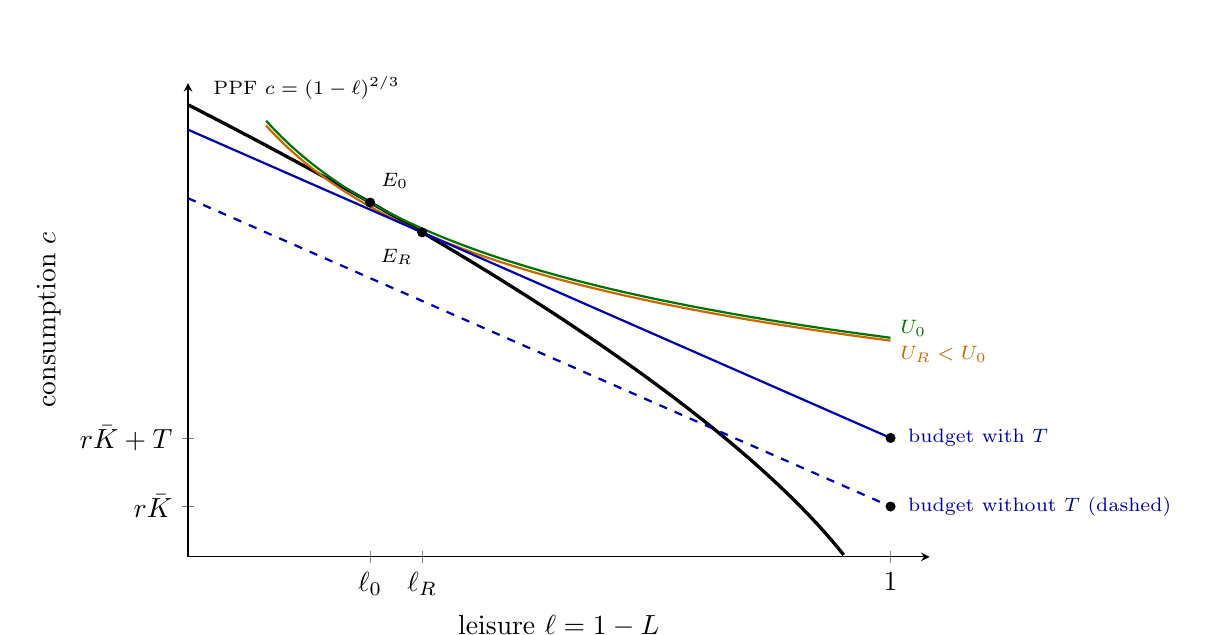
\begin{tikzpicture}
\begin{axis}[width=11cm,height=7.6cm,axis lines=left,xmin=0.1,xmax=1.05,ymin=0.15,ymax=0.97,clip=false,
  xlabel={leisure $\ell=1-L$},ylabel={consumption $c$},xtick={0.3333,0.4,1},xticklabels={$\ell_0$,$\ell_R$,$1$},
  ytick={0.2371,0.3557},yticklabels={$r\bar K$,$r\bar K+T$}]
\addplot[very thick,black,domain=0.1:0.94,samples=120]{(1-x)^(2/3)};
\addplot[thick,green!45!black,domain=0.2:1,samples=80]{0.52912*x^(-1/3)};
\addplot[thick,orange!80!black,domain=0.2:1,samples=80]{0.52418*x^(-1/3)};
\addplot[thick,blue!70!black,domain=0.1:1]{0.3557+0.5928*(1-x)};
\addplot[thick,blue!70!black,dashed,domain=0.1:1]{0.2371+0.5928*(1-x)};
\addplot[only marks,mark=*,mark size=1.6pt] coordinates {(0.3333,0.7631) (0.4,0.7114) (1,0.3557) (1,0.2371)};
\node[font=\scriptsize,anchor=south west] at (axis cs:0.335,0.77) {$E_0$};
\node[font=\scriptsize,anchor=north east] at (axis cs:0.40,0.70) {$E_R$};
\node[font=\scriptsize,anchor=south west] at (axis cs:0.12,0.925) {PPF $c=(1-\ell)^{2/3}$};
\node[font=\scriptsize,green!45!black,anchor=west] at (axis cs:1,0.545) {$U_0$};
\node[font=\scriptsize,orange!80!black,anchor=west] at (axis cs:1,0.50) {$U_R<U_0$};
\node[font=\scriptsize,blue!70!black,anchor=west] at (axis cs:1.01,0.3557) {budget with $T$};
\node[font=\scriptsize,blue!70!black,anchor=west] at (axis cs:1.01,0.2371) {budget without $T$ (dashed)};
\end{axis}
\end{tikzpicture}\\
{\footnotesize $E_0$: the indifference curve $U_0$ is tangent to the frontier (MRS $=$ MPL). $E_R$: the household is
tangent to its after-tax budget line (slope $(1-\tau)w=0.59$), which is flatter than the frontier there
(MPL $=w=0.79$), so the frontier \emph{crosses} $U_R$: there are feasible points above $U_R$. The tax rotates the
budget line about the no-work point $(1,r\bar K)$; the transfer shifts it up in parallel by $T$.}
\end{center}
\intuicao{The rebate gives the money back, but not the incentive: households still see 75 centavos for every real
their hour produces, so they buy too much leisure.}
\refbib{Kurlat ch.~7, \S7.2 (taxes and labour supply), pp.~131--137; related, not the same: ex.~7.5
\emph{Prescott's Calculation}, p.~148; ch.~9, \S9.2.}
\rubrica{
\item FOC with $(1-\tau)w$ and $c=Y$ from the government budget: 0.2. $L_R=0.6$ with the general formula and its
sign: 0.15 (slip: $-0.1$).
\item Why the transfer does not undo the wedge: 0.15. Claiming the rebate makes the tax neutral: max.\ 0.3 on the item.
\item Graph: axes, frontier, two indifference curves, tangency at $E_0$: 0.1; budget line rotated about the
no-work point and shifted by $T$, crossing argument at $E_R$: 0.1. Shifting the budget parallel for the tax: $-0.1$.
}
\end{sol}

\parte{c}{0.6 point} Instead, the same 25\% tax finances government purchases $G=\tau wL$ that give households
no utility ($T=0$). Find $L$. Using (a) and (b), split the change in hours relative to $\tau=0$ into a substitution
effect and an income effect, and explain why hours fall less than in (b). What happens if $\alpha=0$? An economist
argues: ``Labour taxes spent by the government barely change hours, so they cause almost no distortion.''
Evaluate, comparing with financing the same $G$ through a lump-sum tax.
\resolespaco
\begin{sol}
\begin{notacao}
\item Symbols of (a)--(b) keep their meaning. New here:
\item $G=\tau wL\ge0$: government purchases, which give no utility; now $T=0$.
\item $L_G$: hours when the tax finances $G$.
\item Substitution effect: change in $L$ from a change in the after-tax wage with income held fixed;
income effect: change in $L$ from the change in income alone.
\end{notacao}
\passo{1 --- equilibrium}{With $T=0$ and $\Pi=0$ \eqref{q2a:pi}, \eqref{q2:BC} becomes, using $wL+r\bar K=Y$
(Step 2 of (b)) and $wL=(1-\alpha)Y$ from \eqref{q2a:w}:
\begin{align}
c &= (1-\tau)wL+r\bar K+(0)+(0)\nonumber\\
&= (wL+r\bar K)-\tau wL\nonumber\\
&= (Y)-\tau wL\nonumber\\
&= Y-\tau\big((1-\alpha)Y\big)\nonumber\\
&= Y\,[1-\tau(1-\alpha)]. \label{q2c:c}
\end{align}
Numbers: $1-0.25\cdot\tfrac23=\tfrac56$, so $c=\tfrac56Y$ (goods clearing $c+G=Y$ gives the same).
The FOC \eqref{q2b:hh} still holds. Substitute \eqref{q2c:c} and \eqref{q2a:w} into it:
\begin{align*}
\frac{\psi\,\big([1-\tau(1-\alpha)]Y\big)}{1-L} &= (1-\tau)\left(\frac{(1-\alpha)Y}{L}\right)\\
\psi[1-\tau(1-\alpha)]\,L &= (1-\tau)(1-\alpha)(1-L).
\end{align*}
Solve for $L$:
\begin{equation}
\boxed{L_G=\frac{(1-\tau)(1-\alpha)}{\psi[1-\tau(1-\alpha)]+(1-\tau)(1-\alpha)}}. \label{q2c:LG}
\end{equation}
Numbers: $\psi[1-\tau(1-\alpha)]=\tfrac13\cdot\tfrac56=\tfrac{5}{18}$ and $(1-\tau)(1-\alpha)=0.5=\tfrac{9}{18}$:
\[
L_G=\frac{9/18}{\frac{5}{18}+\frac{9}{18}}=\boxed{\tfrac{9}{14}=0.643}.
\]
Then, by \eqref{q2:F}, \eqref{q2a:w} and \eqref{q2c:c}:
\begin{align*}
Y &= (9/14)^{2/3}=0.7449,\\
G &= \tau(1-\alpha)Y=\tfrac16(0.7449)=0.1241,\\
c &= \tfrac56(0.7449)=0.6207.
\end{align*}}
\passo{2 --- decomposition}{(b) changes the price of leisure but gives the income back: it isolates the
\textbf{substitution effect}. From \eqref{q2b:LR} and \eqref{q2a:L0}:
\[
L_R-L_0=0.600-0.667=\boxed{-0.067}.
\]
(c) has the same price change and also takes the income away: the step from (b) to (c) is the
\textbf{income effect}. From \eqref{q2c:LG} and \eqref{q2b:LR}:
\[
L_G-L_R=0.643-0.600=\boxed{+0.043}
\]
(poorer households buy less leisure, a normal good). Total:
\[
L_G-L_0=0.643-0.667=\boxed{-0.024}.
\]}
\passo{3 --- why less, and $\alpha=0$}{The two effects have opposite signs. With log utility they cancel only if
all income is taxed labour income. Here capital income $r\bar K$ is untaxed, so the income loss is smaller than
the price change: substitution wins and hours fall, but by less. Set $\alpha=0$ in \eqref{q2c:LG}:
\begin{align*}
L_G &= \frac{(1-\tau)(1-0)}{\psi[1-\tau(1-0)]+(1-\tau)(1-0)}\\
&= \frac{1-\tau}{\psi(1-\tau)+(1-\tau)}\\
&= \frac{1}{1+\psi},
\end{align*}
\textbf{independent of $\tau$}: exact cancellation.}
\passo{4 --- the economist}{Wrong. The distortion is the wedge MRS $=(1-\tau)$MPL, and its cost is driven by the
\emph{substitution} effect, not by the total response of hours. Benchmark: the same $G=0.1241$ raised lump-sum
leaves MRS $=$ MPL, so \eqref{q2a:hh} with $c=Y-G$ and \eqref{q2a:w} give
\begin{equation}
\frac{\psi(Y-G)}{1-L}=\frac{(1-\alpha)Y}{L}. \label{q2c:ls}
\end{equation}
Solving \eqref{q2c:ls} numerically gives $L=0.703$, more hours than at $\tau=0$ (pure income effect), and higher
utility: $-0.8104$ vs $-0.8201$, a consumption-equivalent gap of about $1.0\%$. Hours barely move under the
labour tax because two effects offset, not because nothing is distorted.}
\intuicao{The observer sees the total change in hours; welfare depends on the compensated change. A tax can leave
hours almost unchanged and still be costly, because it is the gap between what an hour produces and what it pays
that wastes resources.}
\refbib{Kurlat ch.~7, \S7.2 (income and substitution effects; log case), pp.~131--137; ch.~9, \S9.2.}
\rubrica{
\item $L_G=9/14$ with $c=Y[1-\tau(1-\alpha)]$: 0.2 (slip: $-0.1$).
\item Decomposition with signs and the reason (each effect named): 0.15. Reversing the labels: max.\ 0.1 on this line.
\item Why smaller here and the $\alpha=0$ case: 0.1.
\item Economist: wedge and compensated effect, with the lump-sum benchmark: 0.15. Conceding the claim: 0 on this line.
}
\end{sol}

\parte{d}{0.5 point} Return to the rebated tax of (b). Compute the welfare cost of the 25\% tax as the
percentage increase in consumption, at the allocation of (b), that would give households the utility of (a).
Show that the cost is of second order in $\tau$ (that a small tax has a much smaller cost) and check it with
$\tau=12.5\%$. Which instrument would avoid the cost?
\resolespaco
\begin{sol}
\begin{notacao}
\item Symbols of (a)--(b) keep their meaning. New here:
\item $U(L)$: utility as a function of hours when $c=Y$. $U_0$, $U_R$: its values in (a) and (b).
\item $\lambda\ge0$: welfare cost, the proportional rise in consumption at the allocation of (b) that gives
utility $U_0$.
\item $L_R(\tau)$: hours under the rebated tax as a function of $\tau$, from \eqref{q2b:LR}.
\end{notacao}
\passo{1 --- utility}{In both economies $c=Y$ (\eqref{q2a:goods}, \eqref{q2b:cY}) and, by \eqref{q2:F} with
$A\bar K^{\alpha}=1$, $Y=L^{2/3}$. Substitute into \eqref{q2:U}:
\begin{align}
U(L) &= \ln\big(L^{2/3}\big)+\tfrac13\ln(1-L)\nonumber\\
&= \tfrac23\ln L+\tfrac13\ln(1-L). \label{q2d:U}
\end{align}
Evaluate \eqref{q2d:U} at $L_0=\tfrac23$ and $L_R=0.6$:
\begin{align*}
U_0 &= \tfrac23\ln\tfrac23+\tfrac13\ln\tfrac13\\
&= (-0.27031)+(-0.36620)\\
&= -0.63651,\\
U_R &= \tfrac23\ln0.6+\tfrac13\ln0.4\\
&= (-0.34055)+(-0.30543)\\
&= -0.64598.
\end{align*}}
\passo{2 --- consumption equivalent}{By definition of $\lambda$:
\begin{equation}
\ln\big((1+\lambda)c_R\big)+\psi\ln(1-L_R)=U_0. \label{q2d:lam}
\end{equation}
Split the log in \eqref{q2d:lam} and use $U_R=\ln c_R+\psi\ln(1-L_R)$:
\begin{align*}
\ln(1+\lambda)+\big(\ln c_R+\psi\ln(1-L_R)\big) &= U_0\\
\ln(1+\lambda)+(U_R) &= U_0\\
\ln(1+\lambda) &= U_0-U_R\\
&= (-0.63651)-(-0.64598)\\
&= 0.00947,
\end{align*}
and $\lambda=e^{(0.00947)}-1=\boxed{0.95\%}$ of consumption.}
\passo{3 --- second order}{Welfare as a function of the tax is
\begin{equation}
U(\tau)=U\big(L_R(\tau)\big). \label{q2d:Utau}
\end{equation}
$L_0=L_R(0)$ maximises \eqref{q2d:U}: it is the planner's problem \eqref{q2a:plan}. Differentiate
\eqref{q2d:Utau} at $\tau=0$:
\begin{align*}
\frac{dU}{d\tau}\Big|_{\tau=0} &= U'(L_0)\,L_R'(0)\\
&= (0)\cdot L_R'(0)=0
\end{align*}
(envelope argument). The first-order term vanishes, and a second-order expansion of \eqref{q2d:Utau} leaves
\begin{equation}
U_0-U(\tau)\approx\tfrac12|U''(L_0)|\,[L_R'(0)]^2\tau^2, \label{q2d:harb}
\end{equation}
the Harberger triangle. Check: at $\tau=12.5\%$ the cost is $0.20\%$, about a fifth of $0.95\%$, close to the
quarter that \eqref{q2d:harb} predicts (the rest is higher-order terms).}
\passo{4 --- instrument}{A lump-sum tax (here, simply not taxing and not transferring): it does not touch the
marginal trade-off, so MRS $=$ MPL holds and the First Welfare Theorem applies again.}
\intuicao{At the efficient point the first hour moved has no value, so a small wedge costs almost nothing; the cost
grows with the square of the wedge, which is why many small taxes beat one large one.}
\refbib{Kurlat ch.~9, \S9.2 (welfare and taxes), pp.~168--172; ch.~7, \S7.2.}
\rubrica{
\item $U_0$, $U_R$ and $\lambda=0.95\%$: 0.2 (slip: $-0.1$). Comparing utils without converting: max.\ 0.1 on this line.
\item Envelope argument for the second-order cost: 0.15; $\tau=12.5\%$ check: 0.05.
\item Lump-sum tax as the first-best instrument: 0.1.
}
\gap{Kurlat ch.~7 and ch.~9 were absent from Prova 01; Prova 01, 2.c--2.d (list every income source, including
capital income and profits, and every choice variable).}
\end{sol}

% =============================================================================
\questao{(2.5 points) The Real plan, the trip to the bank and the inflation tax.
A stylised Brazil in the early 1990s. A representative household spends its real income $Y$ per year at a constant
rate. It keeps its wealth in an account that pays the nominal rate $i$ and withdraws cash $N$ times a year, in equal
amounts; cash pays no interest. Each trip to the bank costs $F$ in goods (queue, fee, time), that is $pF$ in money.
Take $Y=60{,}000$ (reais of constant purchasing power per year) and $F=25$. In the long run real output grows at
$g=4\%$ a year, the real interest rate is $r=3\%$ and the money supply grows at $\mu=11\%$ a year. Treat all money
as currency (money multiplier equal to one) and use Kurlat's Fisher equation $i=r+\pi$.}

\parte{a}{0.6 point} Derive the optimal number of trips $N$ and the demand for real money balances $M/p$ from the
household's cost minimisation. Find the income and interest elasticities of money demand and the velocity of
money. Compute $N$, $M/p$ and velocity at $i=12\%$. Show graphically how money demand depends on $i$, and how a
fall in $F$ (more ATMs) moves it.
\resolespaco
\begin{sol}
\begin{notacao}
\item $Y>0$: real income per year, spent at a constant rate ($Y=60{,}000$). $p>0$: price level.
\item $i>0$: nominal interest rate on the account; cash pays nothing.
\item $N>0$: withdrawals per year (an integer $\ge1$ in practice); $N^*$ the optimum.
\item $F>0$: real cost of one trip to the bank ($F=25$), so $pF$ in money.
\item $M$: average nominal cash held; $m\equiv M/p$: real money balances.
\item $\mathcal C(N)$: annual nominal cost of managing cash.
\item $\eta$: income elasticity of money demand. $V$: velocity of money.
\end{notacao}
\passo{1 --- the costs}{Each withdrawal is $pY/N$, spent at a constant rate down to zero, so average cash is
half of it:
\begin{equation}
M=\frac{pY}{2N}. \label{q3a:M}
\end{equation}
Annual cost: forgone interest on that cash plus the trips:
\begin{equation}
\mathcal C(N)=\frac{i\,pY}{2N}+pFN. \label{q3a:cost}
\end{equation}}
\passo{2 --- FOC}{Differentiate \eqref{q3a:cost} with respect to $N$ and set it to zero:
\begin{equation}
\mathcal C'(N)=-\frac{ipY}{2N^2}+pF=0. \label{q3a:foc}
\end{equation}
Solve \eqref{q3a:foc} for $N$:
\begin{equation}
\boxed{N^*=\sqrt{\frac{iY}{2F}}} \label{q3a:N}
\end{equation}
(SOC: $\mathcal C''=ipY/N^3>0$). Divide \eqref{q3a:M} by $p$ and substitute \eqref{q3a:N}:
\begin{align}
\frac{M}{p} &= \frac{Y}{2N^*}\nonumber\\
&= \frac{Y}{2\left(\sqrt{\frac{iY}{2F}}\right)}\nonumber\\
&= \frac{Y}{2}\sqrt{\frac{2F}{iY}}\nonumber\\
&= \sqrt{\frac{FY}{2i}}. \label{q3a:md}
\end{align}}
\passo{3 --- elasticities and velocity}{Take the log of \eqref{q3a:md}:
\begin{equation}
\ln\frac Mp=\tfrac12\ln\frac F2+\tfrac12\ln Y-\tfrac12\ln i. \label{q3a:ln}
\end{equation}
The coefficients in \eqref{q3a:ln} are the elasticities: income elasticity $\boxed{\eta=\tfrac12}$, interest
elasticity $\boxed{-\tfrac12}$ (economies of scale in cash management). Velocity, using the first line of
\eqref{q3a:md} and then \eqref{q3a:N}:
\begin{align}
V\equiv\frac{pY}{M} &= \frac{Y}{M/p}\nonumber\\
&= \frac{Y}{\left(\frac{Y}{2N^*}\right)}\nonumber\\
&= 2N^*\nonumber\\
&= 2\left(\sqrt{\frac{iY}{2F}}\right)\nonumber\\
&= \sqrt{\frac{2iY}{F}}: \label{q3a:V}
\end{align}
not a constant; it rises with $i$ and $Y$.}
\passo{4 --- numbers}{At $i=0.12$, by \eqref{q3a:N}, \eqref{q3a:md} and \eqref{q3a:V}:
\begin{align*}
N^* &= \sqrt{\frac{0.12\cdot60{,}000}{2\cdot25}}=\sqrt{144}=\boxed{12}\ \text{trips a year},\\
\frac Mp &= \frac{60{,}000}{2\cdot12}=\frac{60{,}000}{24}=\boxed{2{,}500},\\
V &= 2\cdot12=\boxed{24}.
\end{align*}}
\begin{center}
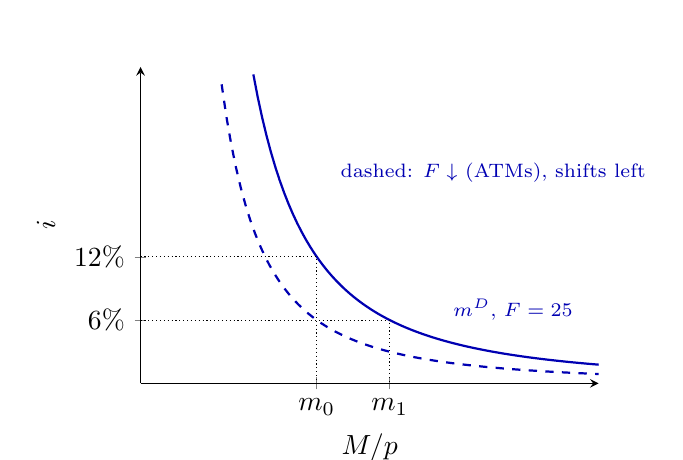
\begin{tikzpicture}
\begin{axis}[width=7.4cm,height=5.6cm,axis lines=left,xmin=0,xmax=6500,ymin=0,ymax=0.3,
  xlabel={$M/p$},ylabel={$i$},xtick={2500,3535.5},xticklabels={$m_0$,$m_1$},ytick={0.06,0.12},
  yticklabels={6\%,12\%},scaled x ticks=false,clip=false]
\addplot[thick,blue!70!black,domain=1600:6500,samples=80]{750000/x^2};
\addplot[thick,blue!70!black,dashed,domain=1150:6500,samples=80]{375000/x^2};
\addplot[densely dotted] coordinates {(0,0.12) (2500,0.12) (2500,0)};
\addplot[densely dotted] coordinates {(0,0.06) (3535.5,0.06) (3535.5,0)};
\node[font=\scriptsize,blue!70!black,anchor=west] at (axis cs:4300,0.07) {$m^D$, $F=25$};
\node[font=\scriptsize,blue!70!black,anchor=west] at (axis cs:2700,0.2) {dashed: $F\downarrow$ (ATMs), shifts left};
\end{axis}
\end{tikzpicture}
\end{center}
{\footnotesize Downward-sloping in $i$ (elasticity $-\tfrac12$); a lower $F$ shifts the whole curve left
(fewer balances at every $i$). Points used in (b): $i=12\%$ and $6\%$.}
\intuicao{Holding cash costs interest; refilling it costs trips. Doubling spending does not double cash, because the
trip cost is fixed: the optimal number of trips rises too.}
\refbib{Kurlat ch.~10, \S10.4, pp.~199--204, eqs.~(10.4.3)--(10.4.4); the exercise on ATMs, ex.~10.4, p.~203,
is related practice.}
\rubrica{
\item Average cash $pY/2N$ and the cost function: 0.15. $N^*$ and $M/p$ derived: 0.15.
\item Both elasticities and $V=2N$: 0.1. Numbers 12, 2{,}500, 24: 0.1 (slip: $-0.1$).
\item Graph with $i$ and $M/p$ on the axes and the shift for $F\downarrow$: 0.1.
\item Quoting $\sqrt{FY/2i}$ without deriving it: max.\ 0.2 on the item.
}
\end{sol}

\parte{b}{0.7 point} Using money-market equilibrium $M=p\,m^D(Y,i)$, derive the steady-state inflation rate when
$Y$ grows at $g$ and $i$ is constant, and compute $\pi$ and $i$. In mid-1994 the central bank cuts money growth
permanently and credibly to $\mu=5\%$. Find the new $\pi$ and $i$ and the change in real balances. Since the stock
of money does not jump by itself, what must happen to the price level on the day of the reform? Which one-time
change in $M$ would avoid it? Draw $\ln M$ and $\ln p$ around the reform, with that one-time change. A commentator
writes: ``After the Real, M1 rose by tens of percent while inflation collapsed, so money does not cause inflation.''
Evaluate.
\resolespaco
\begin{sol}
\begin{notacao}
\item Symbols of (a) keep their meaning. New here:
\item $m^D(Y,i)$: real money demand, \eqref{q3a:md}. A dot is a time derivative ($\dot M=dM/dt$).
\item $\mu\equiv\dot M/M$: money growth. $\pi\equiv\dot p/p$: inflation. $g\equiv\dot Y/Y$: real growth.
$r$: real interest rate. All per year.
\item $T$: date of the reform. $m_0$, $m_1$: real balances before and after; $p_{\text{old}}$, $p_{\text{new}}$:
price level just before and just after.
\end{notacao}
\passo{1 --- differentiate}{Money-market equilibrium at every date:
\begin{equation}
M_t=p_t\,m^D(Y_t,i_t). \label{q3b:mm}
\end{equation}
Differentiate \eqref{q3b:mm} with respect to $t$:
\begin{equation}
\dot M=\dot p\,m^D+p\Big(\frac{\partial m^D}{\partial Y}\dot Y+\frac{\partial m^D}{\partial i}\dot i\Big).
\label{q3b:diff}
\end{equation}
Set $\dot i=0$ and divide \eqref{q3b:diff} by \eqref{q3b:mm}:
\begin{align}
\frac{\dot M}{M} &= \frac{\dot p\,m^D+p\big(\frac{\partial m^D}{\partial Y}\dot Y+\frac{\partial m^D}{\partial i}(0)\big)}{p\,m^D}
\nonumber\\
&= \frac{\dot p}{p}+\underbrace{\frac{\partial m^D}{\partial Y}\frac{Y}{m^D}}_{\eta}
\frac{\dot Y}{Y}\nonumber\\
\mu &= \pi+\eta g\nonumber\\
\pi &= \mu-\eta g, \label{q3b:pi}
\end{align}
with $\eta=\tfrac12$ from \eqref{q3a:ln}. Kurlat's Fisher equation, from the statement:
\begin{equation}
i=r+\pi. \label{q3b:fisher}
\end{equation}}
\passo{2 --- before}{By \eqref{q3b:pi} and then \eqref{q3b:fisher}:
\begin{align*}
\pi &= 11\%-\tfrac12(4\%)=\boxed{9\%},\\
i &= 3\%+9\%=\boxed{12\%}
\end{align*}
(exact Fisher: $1.03\cdot1.09-1=12.27\%$).}
\passo{3 --- after}{With $\mu=5\%$, by \eqref{q3b:pi} and \eqref{q3b:fisher}:
\begin{align*}
\pi &= 5\%-\tfrac12(4\%)=\boxed{3\%},\\
i &= 3\%+3\%=\boxed{6\%}
\end{align*}
(Fisher effect: $i$ falls one-for-one with $\pi$, $r$ unchanged). Real balances, from the ratio of
\eqref{q3a:md} at the two rates:
\begin{align*}
\frac{m_1}{m_0} &= \frac{\sqrt{FY/(2i_1)}}{\sqrt{FY/(2i_0)}}\\
&= \sqrt{\frac{i_0}{i_1}}\\
&= \sqrt{\frac{0.12}{0.06}}\\
&= \sqrt2=1.414,
\end{align*}
$\boxed{+41.4\%}$ ($2{,}500\to3{,}536$). The jump is immediate: a credible reform changes expected inflation,
hence $i$, at once.}
\passo{4 --- the price level}{Solve \eqref{q3b:mm} for the price level:
\begin{equation}
p=\frac{M}{m^D}. \label{q3b:p}
\end{equation}
If $M$ is continuous and $m^D$ jumps by $\sqrt2$, \eqref{q3b:p} makes $p$ jump \emph{down}:
\begin{align*}
\frac{p_{\text{new}}}{p_{\text{old}}} &= \frac{M/m_1}{M/m_0}\\
&= \frac{m_0}{m_1}\\
&= \frac{1}{\sqrt2}=0.707,
\end{align*}
a $\boxed{29.3\%}$ fall in the price level. To keep $p$ continuous in \eqref{q3b:p}, $M$ must jump with $m^D$:
the central bank issues a one-time injection
\[
\boxed{\frac{\Delta M}{M}=\sqrt2-1=41.4\%}
\]
on the day of the reform (remonetisation), and \emph{from then on} money grows at 5\%. This injection is not
inflationary: it only meets the higher demand for real balances.}
\begin{center}
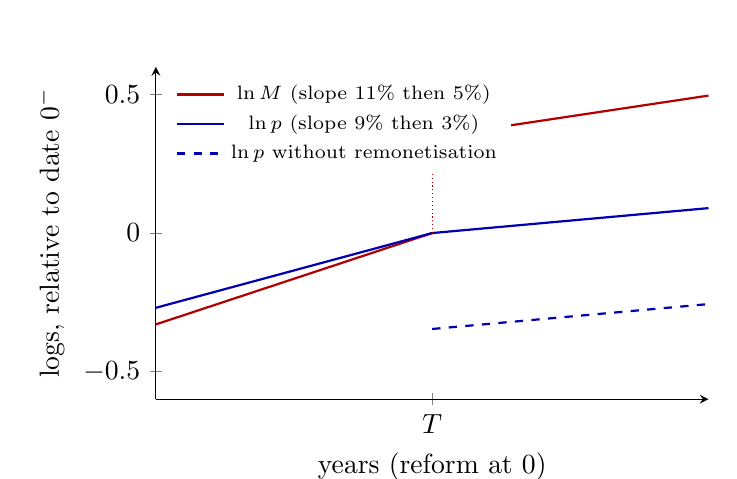
\begin{tikzpicture}
\begin{axis}[width=8.6cm,height=5.8cm,axis lines=left,xmin=-3,xmax=3,ymin=-0.6,ymax=0.6,
  xlabel={years (reform at $0$)},ylabel={logs, relative to date $0^-$},xtick={0},xticklabels={$T$},
  legend style={font=\scriptsize,draw=none,at={(0.02,0.98)},anchor=north west}]
\addplot[thick,red!70!black] coordinates {(-3,-0.33) (0,0)};
\addplot[thick,blue!70!black] coordinates {(-3,-0.27) (0,0)};
\addplot[thick,blue!70!black,dashed] coordinates {(0,-0.3466) (3,-0.2566)};
\addplot[thick,red!70!black,forget plot] coordinates {(0,0.3466) (3,0.4966)};
\addplot[thick,blue!70!black,forget plot] coordinates {(0,0) (3,0.09)};
\addplot[densely dotted,red!70!black,forget plot] coordinates {(0,0) (0,0.3466)};
\legend{$\ln M$ (slope 11\% then 5\%),$\ln p$ (slope 9\% then 3\%),$\ln p$ without remonetisation}
\end{axis}
\end{tikzpicture}\\
{\footnotesize With remonetisation $\ln M$ jumps by $\ln\sqrt2=0.35$ and $\ln p$ only changes slope. Without it,
$\ln M$ is continuous and $\ln p$ jumps down by $0.35$.}
\end{center}
\passo{5 --- the commentator}{Wrong inference. \eqref{q3b:pi} holds \emph{with $i$ constant}; at the reform $i$
falls and real money demand rises by about 41\%, so a one-time rise in $M$ of that size is exactly what keeps
prices stable. It is a \emph{level} adjustment of $M$ to a higher $m^D$, not sustained money growth. The theory
predicts both facts at once: the money stock jumps and inflation falls, because $\mu$ after the jump is low.}
\intuicao{When people expect inflation to fall, holding cash becomes cheaper and they want more of it. Either the
central bank supplies that cash, or prices fall until existing cash is worth enough.}
\refbib{Kurlat ch.~11, \S11.2, pp.~209--212, eq.~(11.2.3); \S11.1--\S11.2 on neutrality, pp.~205--215.}
\rubrica{
\item Total differentiation with $\dot i=0$ stated and $\eta$ named: 0.15. $\pi=9\%$, $i=12\%$: 0.05.
\item $\pi=3\%$, $i=6\%$, $m$ up by $\sqrt2$: 0.15. Using $\eta=1$ (quantity theory) instead of $\tfrac12$: $-0.1$.
\item Price-level jump of $-29.3\%$ or remonetisation of $41.4\%$: 0.15. Graph (slopes and the jump): 0.1.
\item Commentator: level vs growth, $m^D$ rising with lower $i$: 0.1. Agreeing with the commentator: 0 on this line.
}
\end{sol}

\parte{c}{0.6 point} Seigniorage. Compute real seigniorage per household before and after the reform, and split it
into the inflation tax and the part due to growth. Show that with the money demand of (a) seigniorage rises with
$\mu$ for every $\mu$, so there is no revenue-maximising money growth. Contrast with a Cagan semi-log demand
$M/p=Y e^{-a i}$, $a>0$: find the revenue-maximising $\mu$ and evaluate it for $a=2$. Draw both curves. Which demand
is consistent with Brazil's 1989--1993 experience, when money grew by more than 1{,}000\% a year?
\resolespaco
\begin{sol}
\begin{notacao}
\item Symbols of (a)--(b) keep their meaning. New here:
\item $S$: real seigniorage per household per year, the real value of newly issued money.
\item $a>0$: semi-elasticity of the Cagan demand $M/p=Ye^{-ai}$ with respect to $i$ ($a=2$).
\item $\mu^{\max}$: the money growth that maximises $S$ (the peak of the seigniorage Laffer curve).
\end{notacao}
\passo{1 --- definition}{Real seigniorage, multiplying and dividing by $M$:
\begin{align}
S\equiv\frac{\dot M}{p} &= \frac{\dot M}{M}\cdot\frac{M}{p}\nonumber\\
&= \mu\,m. \label{q3c:S}
\end{align}
Substitute $\mu=\pi+\eta g$ from \eqref{q3b:pi} into \eqref{q3c:S}:
\begin{align}
S &= (\pi+\eta g)\,m\nonumber\\
&= \underbrace{\pi m}_{\text{inflation tax}}+\underbrace{\eta g\,m}_{\text{growth}}. \label{q3c:split}
\end{align}}
\passo{2 --- numbers}{Before ($\mu=11\%$, $\pi=9\%$, $m=2{,}500$), by \eqref{q3c:S} and \eqref{q3c:split}:
\begin{align*}
S &= 0.11\cdot2{,}500=\boxed{275},\\
\pi m+\eta g\,m &= 0.09\cdot2{,}500+\tfrac12(0.04)\cdot2{,}500=225+50,
\end{align*}
$0.46\%$ of $Y$. After ($\mu=5\%$, $\pi=3\%$, $m=3{,}536$):
\begin{align*}
S &= 0.05\cdot3{,}536=\boxed{176.8},\\
\pi m+\eta g\,m &= 0.03\cdot3{,}536+\tfrac12(0.04)\cdot3{,}536=106.1+70.7,
\end{align*}
$0.29\%$ of $Y$. Revenue falls by 36\%, much less than $\mu$ (by 55\%), because the base rises 41\%; and the
growth part \emph{rises}: a growing economy absorbs new money without inflation.}
\passo{3 --- no peak under Baumol--Tobin}{Substitute \eqref{q3b:pi} into \eqref{q3b:fisher}:
\begin{align}
i &= r+(\mu-\eta g)\nonumber\\
&= 0.03+\mu-\tfrac12(0.04)\nonumber\\
&= \mu+0.01. \label{q3c:i}
\end{align}
Substitute \eqref{q3a:md} with \eqref{q3c:i} into \eqref{q3c:S}:
\begin{align}
S &= \mu\left(\sqrt{\frac{FY}{2i}}\right)\nonumber\\
S(\mu) &= \mu\sqrt{\frac{FY}{2(\mu+r-\eta g)}}. \label{q3c:Sbt}
\end{align}
Differentiate the log of \eqref{q3c:Sbt}, using $di/d\mu=1$ and $2i-\mu=\mu+2(r-\eta g)$:
\begin{align*}
\frac{d\ln S}{d\mu} &= \frac1\mu-\frac{1}{2i}\\
&= \frac{2i-\mu}{2\mu i}\\
&= \frac{2(\mu+r-\eta g)-\mu}{2\mu i}\\
&= \frac{\mu+2(r-\eta g)}{2\mu i}>0
\end{align*}
for all $\mu>0$, since $r-\eta g=1\%>0$. Equivalently, the elasticity of the base with respect to $\mu$ is $-\mu/(2i)>-\tfrac12>-1$: the base never shrinks
fast enough to offset the rate. \#~The Laffer peak needs a base elasticity of $-1$.}
\passo{4 --- Cagan}{The Cagan demand:
\begin{equation}
\frac Mp=Ye^{-ai}. \label{q3c:cagan}
\end{equation}
Substitute \eqref{q3c:cagan} with \eqref{q3c:i} into \eqref{q3c:S}:
\begin{align}
S &= \mu\big(Ye^{-ai}\big)\nonumber\\
&= \mu Y e^{-a(r-\eta g+\mu)}. \label{q3c:Scagan}
\end{align}
Differentiate \eqref{q3c:Scagan} with respect to $\mu$ and set it to zero:
\begin{align*}
\frac{dS}{d\mu} &= Ye^{-a(\cdot)}\,(1-a\mu)=0\\
\Rightarrow\ \mu^{\max} &= 1/a.
\end{align*}
SOC: $\frac{d^2S}{d\mu^2}=-aYe^{-a(\cdot)}(2-a\mu)<0$ at $\mu=1/a$. With $a=2$:
$\boxed{\mu^{\max}=1/a=1/2=50\%}$ a year.}
\begin{center}
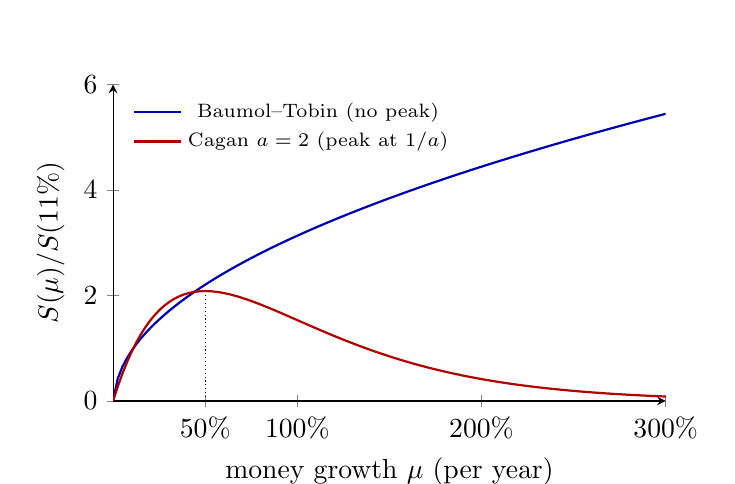
\begin{tikzpicture}
\begin{axis}[width=8.6cm,height=5.6cm,axis lines=left,xmin=0,xmax=3,ymin=0,ymax=6,
  xlabel={money growth $\mu$ (per year)},ylabel={$S(\mu)/S(11\%)$},xtick={0.5,1,2,3},
  xticklabels={50\%,100\%,200\%,300\%},
  legend style={font=\scriptsize,draw=none,at={(0.02,0.98)},anchor=north west}]
\addplot[thick,blue!70!black,domain=0:3,samples=120]{x/sqrt(x+0.01)/0.31754};
\addplot[thick,red!70!black,domain=0:3,samples=120]{x*exp(-2*(x+0.01))/0.086530};
\addplot[densely dotted] coordinates {(0.5,0) (0.5,2.0837)};
\legend{Baumol--Tobin (no peak),Cagan $a=2$ (peak at $1/a$)}
\end{axis}
\end{tikzpicture}
\end{center}
\passo{5 --- Brazil}{Rising revenue at any $\mu$, as \eqref{q3c:Sbt} implies, cannot explain why governments
printing over 1{,}000\% a year did not raise ever more revenue; with a Cagan demand \eqref{q3c:Scagan} they were
far on the \emph{wrong side} of the Laffer curve, where cutting $\mu$ costs little revenue or even raises it.
Baumol--Tobin with a fixed $F$ misses the flight from money at high inflation (indexed overnight accounts lowered
the effective $F$ and made demand far more elastic).}
\intuicao{Seigniorage is a tax with rate $\mu$ on the base $M/p$. Whether raising the rate raises revenue depends on
how fast the base flees; under Baumol--Tobin it flees too slowly to ever turn revenue down.}
\refbib{Kurlat ch.~11, \S11.3, pp.~215--216 (seigniorage); the Cagan demand is used in ex.~11.6, p.~218, which
works the limit on revenue with another functional form.}
\rubrica{
\item $S=\mu m$ and the split: 0.1. Both numbers and splits: 0.15 (slip: $-0.1$).
\item Proof of no peak (derivative signed, or elasticity $>-1$): 0.15. Asserting it without proof: 0 on this line.
\item Cagan peak with SOC and 50\%: 0.1. Graph (both curves, peak marked): 0.05.
\item Brazil reading: 0.05.
}
\end{sol}

\parte{d}{0.6 point} Costs of inflation. Compute the real resources spent on trips to the bank, in reais and as a
share of $Y$, before and after the reform. Why is the forgone interest on cash not counted as a cost to society?
Find the inflation and money-growth rates of the Friedman rule, and say what happens to the Baumol--Tobin solution
there. Give two reasons why the central bank targets 3\% rather than this rate.
\resolespaco
\begin{sol}
\begin{notacao}
\item Symbols of (a)--(c) keep their meaning. New here:
\item $R\ge0$: real resources spent on trips to the bank per year (shoe-leather cost), $R=FN^*$.
\item Friedman rule: the policy that sets the nominal interest rate to zero, $i=0$.
\end{notacao}
\passo{1 --- trips}{The resource cost is the number of trips times their real cost. Substitute
\eqref{q3a:N}:
\begin{align}
R=FN^* &= F\left(\sqrt{\frac{iY}{2F}}\right)\nonumber\\
&= \boxed{\sqrt{\frac{iFY}{2}}}. \label{q3d:R}
\end{align}
Before ($i=12\%$, $N^*=12$) and after ($i=6\%$), by \eqref{q3d:R}:
\begin{align*}
R_{\text{before}} &= 25\cdot12=\boxed{300},\quad 0.50\%\ \text{of }Y,\\
R_{\text{after}} &= \sqrt{\frac{0.06\cdot25\cdot60{,}000}{2}}=\sqrt{45{,}000}=\boxed{212.1},\quad 0.35\%\ \text{of }Y.
\end{align*}
The reform saves $0.15\%$ of income every year (shoe-leather cost).}
\passo{2 --- forgone interest}{Multiply \eqref{q3a:md} by $i$: at the optimum the forgone interest is
\[
i\,\frac Mp=i\left(\sqrt{\frac{FY}{2i}}\right)=\sqrt{\frac{iFY}{2}},
\]
the same as \eqref{q3d:R} (300 before), but it is not a use of resources: the inflation-tax part
($\pi m=225$, \eqref{q3c:split}) is revenue of the government, and the rest is a transfer to whoever borrows the
funds. Only the trips burn goods. (Total private cost $\sqrt{2iFY}=600$.)}
\passo{3 --- Friedman rule}{Set $i=0$ in \eqref{q3b:fisher}, then use \eqref{q3b:pi} solved for $\mu$:
\begin{align*}
(0) &= r+\pi\\
\pi &= -r=\boxed{-3\%},\\
\mu &= \pi+\eta g=(-3\%)+\tfrac12(4\%)=\boxed{-1\%}.
\end{align*}
Then, by \eqref{q3a:N} and \eqref{q3a:md}, $N^*\to0$ and $M/p\to\infty$. The interior solution needs $N^*\ge1$;
by \eqref{q3a:N}:
\[
\frac{iY}{2F}\ge1\iff i\ge\frac{2F}{Y}=\frac{2\cdot25}{60{,}000}=0.083\%;
\]
below that the household makes one trip and holds $Y/2=30{,}000$. Shoe-leather costs vanish.}
\passo{4 --- why 3\%}{(i) Measured inflation overstates true inflation (substitution, quality and new-goods biases
of a Laspeyres index), so 0 measured is deflation. (ii) With $\pi=-3\%$, $i$ would sit at zero in normal times,
leaving no room to cut it in a recession --- the zero lower bound of Question 4. (iii) Nominal wages are rigid
downward; some inflation lets real wages fall.}
\intuicao{Inflation is a tax on holding cash; people spend real resources dodging it. The Friedman rule removes the
tax, but a central bank that needs room to cut rates gives up a little of that gain.}
\refbib{Kurlat ch.~11, \S11.4, pp.~216--222 (costs of inflation, Friedman rule); ch.~10, \S10.4.}
\rubrica{
\item Trip cost formula and both numbers with shares: 0.2 (slip: $-0.1$). Counting $i\,m$ as the social cost: max.\ 0.1 on this line.
\item Transfer argument: 0.1. Friedman rule $\pi=-3\%$, $\mu=-1\%$: 0.1; the corner $N\ge1$: 0.05.
\item Two valid reasons for a positive target: 0.15.
}
\gap{Kurlat ch.~10--11 were absent from Prova 01: Baumol--Tobin from primitives, $\pi=\mu-\eta g$ by total
differentiation, Fisher, seigniorage and its Laffer curve.}
\end{sol}

% =============================================================================
\questao{(3.0 points) The Copom between a tax shock and a liquidity trap.
Use Benigno (2015), in log deviations from an efficient steady state, with a short run and a long run:
\begin{align}
y &= \bar y_n+(g-\bar g)-\sigma\left[i-(\bar p-p)-\rho\right], \tag{AD}\label{q4:AD}\\
p-p^e &= \kappa(y-y_n), \tag{AS}\label{q4:AS}\\
y_n &= \frac{(1+\eta)a+\sigma^{-1}g-\mu}{\sigma^{-1}+\eta}, \tag{YN}\label{q4:YN}\\
y_e &= \frac{(1+\eta)a+\sigma^{-1}g}{\sigma^{-1}+\eta}. \tag{YE}\label{q4:YE}
\end{align}
Initially $a=g=\bar g=\mu=0$, $\bar y_n=0$, $\bar p=p^e=0$ and $i=\rho$. Take $\sigma=1$, $\eta=1$, $\kappa=1/2$ and
$\rho=2\%$; $y$ and $p$ are in percent. The Copom sets $i$ to minimise
\begin{equation}
L=\tfrac12(y-y_e)^2+\frac{\phi}{2\kappa}(p-p^e)^2,\qquad \phi>0. \tag{LF}\label{q4:LF}
\end{equation}}

\parte{a}{0.8 point} A temporary rise in a federal tax on firms' revenues raises the mark-up by $\mu=4$ in the
current period only. Find the changes in $y_n$ and $y_e$ and say which curve shifts. Derive the Copom's optimal
targeting rule by substituting the relevant constraint into the loss, and the optimal $y$ and $p$ as functions of
$\phi$; evaluate them for $\phi=4$. Explain why the Copom cannot reach $y=y_e$ and $p=p^e$ together here, while it
could after a temporary productivity shock. Show graphically.
\resolespaco
\begin{sol}
\begin{notacao}
\item $y$, $p$: output and price level today, log deviations from the steady state, in percent.
\item $\bar y_n$, $\bar p$: long-run natural output and long-run price level. $p^e$: the price preset by firms
that cannot adjust this period.
\item $i\ge0$: nominal policy rate, the Copom's instrument. $\rho>0$: rate of time preference, the steady-state
real rate ($\rho=2\%$).
\item $g$, $\bar g$: government spending today and in the long run. $a$: productivity. $\mu$: firms' mark-up
(here raised by the tax).
\item $\sigma>0$: intertemporal elasticity of substitution (not the capital share of Q1). $\eta>0$: inverse
Frisch elasticity of labour supply. $\kappa>0$: slope of AS.
\item $y_n$: natural output (flexible prices, with the mark-up). $y_e$: efficient output (no mark-up).
\item $\phi>0$: weight on price surprises in the loss $L$ \eqref{q4:LF}.
\item $\Delta\equiv y_e-y_n$: the gap between efficient and natural output (defined in Step 1).
\item $y^*$, $p^*$: the optimal point. $E_0$: initial equilibrium. $E'$: the outcome with $i=\rho$. $O$: the optimum.
\end{notacao}
\passo{1 --- what moves}{Differentiate \eqref{q4:YN} and \eqref{q4:YE} with respect to $\mu$:
\begin{align}
dy_n &= -\frac{\mu}{\sigma^{-1}+\eta}=-\frac{4}{1+1}=\boxed{-2}, \label{q4a:dyn}\\
dy_e &= \boxed{0}\qquad(\mu\text{ is not in }y_e). \label{q4a:dye}
\end{align}
\textbf{AS shifts up/left}: by \eqref{q4:AS} it now passes through $(y_n',p^e)=(-2,0)$, so at each $y$ the price
is higher by $\kappa\cdot2=1$. \textbf{AD does not move}: $\mu$ is not in \eqref{q4:AD} and, the shock being
temporary, $\bar y_n$ is unchanged. From \eqref{q4a:dyn}--\eqref{q4a:dye}:
\begin{equation}
\Delta\equiv y_e-y_n=0-(-2)=2>0. \label{q4a:Delta}
\end{equation}}
\passo{2 --- the constraint}{The Copom moves AD with $i$, so it can pick \emph{any} point on AS; AS ($p^e$ is
predetermined) is the constraint. Substitute \eqref{q4:AS} into \eqref{q4:LF}:
\begin{align}
L(y) &= \tfrac12(y-y_e)^2+\frac{\phi}{2\kappa}\big(\kappa(y-y_n)\big)^2\nonumber\\
&= \tfrac12(y-y_e)^2+\frac{\phi}{2\kappa}\kappa^2(y-y_n)^2\nonumber\\
&= \tfrac12(y-y_e)^2+\frac{\phi\kappa}{2}(y-y_n)^2. \label{q4a:Ly}
\end{align}}
\passo{3 --- targeting rule}{Differentiate \eqref{q4a:Ly} and set it to zero (SOC $1+\phi\kappa>0$):
\begin{equation}
\frac{dL}{dy}=(y-y_e)+\phi\kappa(y-y_n)=0. \label{q4a:foc}
\end{equation}
By \eqref{q4:AS}, $\kappa(y-y_n)=p-p^e$. Substitute this into \eqref{q4a:foc}:
\begin{equation}
\boxed{(y-y_e)+\phi\,(p-p^e)=0}. \label{q4a:rule}
\end{equation}
Solve \eqref{q4a:foc} for $y$, then use $y_e=0$ and $y_n=-\Delta$ from \eqref{q4a:Delta}:
\begin{align}
y(1+\phi\kappa) &= y_e+\phi\kappa\,y_n\nonumber\\
y^* &= \frac{y_e+\phi\kappa\,y_n}{1+\phi\kappa}\nonumber\\
&= \frac{(0)+\phi\kappa\,(-\Delta)}{1+\phi\kappa}\nonumber\\
&= -\frac{\phi\kappa\,\Delta}{1+\phi\kappa}. \label{q4a:ystar}
\end{align}
Subtract $y_n=-\Delta$ from \eqref{q4a:ystar} and substitute into \eqref{q4:AS}:
\begin{align}
y^*-y_n &= \left(-\frac{\phi\kappa\,\Delta}{1+\phi\kappa}\right)-(-\Delta)\nonumber\\
&= \frac{\Delta}{1+\phi\kappa},\nonumber\\
p^*-p^e &= \kappa(y^*-y_n)\nonumber\\
&= \kappa\left(\frac{\Delta}{1+\phi\kappa}\right)\nonumber\\
&= \frac{\kappa\,\Delta}{1+\phi\kappa}. \label{q4a:pstar}
\end{align}
With $\phi=4$, $\phi\kappa=2$; by \eqref{q4a:ystar} and \eqref{q4a:pstar}:
\begin{align*}
y^* &= -\frac{2\cdot2}{1+2}=\boxed{-1.33\%},\\
p^* &= \frac{0.5\cdot2}{1+2}=\boxed{+0.33\%}.
\end{align*}
Check in \eqref{q4a:rule}: $-\tfrac43+4\cdot\tfrac13=0$ \checkmark.}
\passo{4 --- divine coincidence fails}{Both targets require $y=y_e=0$ and $p=p^e$, but on the new AS
\eqref{q4:AS}, $p-p^e=\kappa(0+2)=1\neq0$ at $y=0$: the bliss point is not on the constraint, and one instrument
cannot hit two targets. After a temporary productivity shock, \eqref{q4:YN} and \eqref{q4:YE} move $y_n$ and $y_e$
by the same $\frac{1+\eta}{\sigma^{-1}+\eta}a$, so $(y_e,p^e)$ lies on the new AS and the Copom puts AD through it:
zero loss, whatever $\phi$.}
\begin{center}
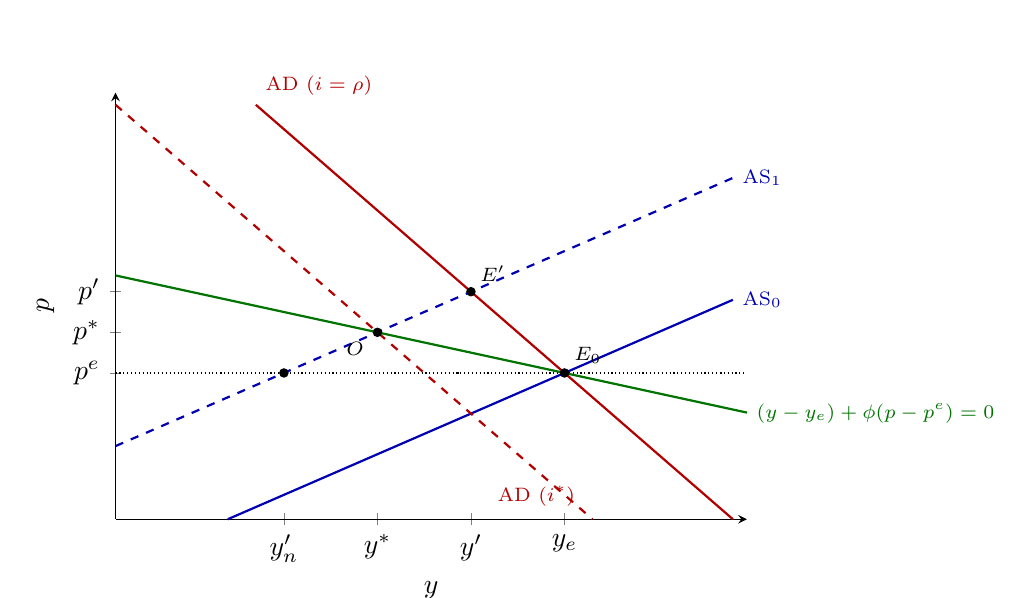
\begin{tikzpicture}
\begin{axis}[width=9.6cm,height=7cm,axis lines=left,xmin=-3.2,xmax=1.3,ymin=-1.2,ymax=2.3,clip=false,
  xlabel={$y$},ylabel={$p$},
  xtick={-2,-1.3333,-0.6667,0},xticklabels={$y_n'$,$y^*$,$y'$,$y_e$},ytick={0,0.3333,0.6667},
  yticklabels={$p^e$,$p^*$,$p'$}]
\addplot[densely dotted,domain=-3.2:1.3]{0};
\addplot[thick,blue!70!black,domain=-2.4:1.2]{0.5*x};
\addplot[thick,blue!70!black,dashed,domain=-3.2:1.2]{0.5*(x+2)};
\addplot[thick,red!70!black,domain=-2.2:1.2]{-x};
\addplot[thick,red!70!black,dashed,domain=-3.2:0.2]{-x-1};
\addplot[thick,green!45!black,domain=-3.2:1.3]{-x/4};
\addplot[only marks,mark=*,mark size=1.5pt] coordinates {(0,0) (-0.6667,0.6667) (-1.3333,0.3333) (-2,0)};
\node[font=\scriptsize,blue!70!black,anchor=west] at (axis cs:1.2,0.6) {AS$_0$};
\node[font=\scriptsize,blue!70!black,anchor=west] at (axis cs:1.2,1.6) {AS$_1$};
\node[font=\scriptsize,red!70!black,anchor=south west] at (axis cs:-2.2,2.2) {AD ($i=\rho$)};
\node[font=\scriptsize,red!70!black,anchor=north] at (axis cs:-0.2,-0.85) {AD ($i^*$)};
\node[font=\scriptsize,green!45!black,anchor=west] at (axis cs:1.3,-0.33) {$(y-y_e)+\phi(p-p^e)=0$};
\node[font=\scriptsize,anchor=south west] at (axis cs:-0.67,0.67) {$E'$};
\node[font=\scriptsize,anchor=north east] at (axis cs:-1.36,0.33) {$O$};
\node[font=\scriptsize,anchor=south west] at (axis cs:0,0) {$E_0$};
\end{axis}
\end{tikzpicture}\\
{\footnotesize AS shifts up through $(y_n',p^e)$; with $i=\rho$ the economy goes to $E'=(-0.67,\,0.67)$ along the
unmoved AD. The optimum $O=(-1.33,\,0.33)$ is where AS$_1$ meets the targeting line (slope $-1/\phi$, through
the bliss point $E_0$); the Copom raises $i$ to move AD down to $O$.}
\end{center}
\intuicao{A mark-up shock makes the economy's natural output inefficiently low. Pushing output up to the efficient
level costs inflation; holding prices costs output. With convex losses the Copom splits the difference, and $\phi$
says how much it dislikes the price side.}
\refbib{Benigno (2015), \S7 (mark-up shocks), Fig.~9, pp.~513--514; \S11, eqs.~(33)--(35), Fig.~14, pp.~521--523;
\S4.2--\S4.4 for $y_n$ vs $y_e$, pp.~508--509.}
\rubrica{
\item $dy_n=-2$, $dy_e=0$, AS shifts and AD does not, with reasons: 0.2. Shifting AD: max.\ 0.3 on the item.
\item Substituting AS into the loss and $dL/dy=0$; the targeting rule: 0.2. Minimising along AD or treating $i$ as
the choice with AD as the constraint: max.\ 0.3 on the item.
\item $y^*$, $p^*$ in general and $-1.33$, $+0.33$: 0.15 (slip: $-0.1$).
\item Divine-coincidence argument and the productivity contrast: 0.1.
\item Graph: axes, AS$_0$/AS$_1$, AD, the targeting line, $E'$ and $O$: 0.15.
}
\end{sol}

\parte{b}{0.6 point} Find the policy rate $i^*$ that implements the optimum, for general $\phi$ and for $\phi=4$, and
compare it with keeping $i=\rho$. Show that the Copom raises the rate if and only if $\phi>\sigma$. Interpret
$\phi\to0$, $\phi\to\infty$ and the knife edge $\phi=\sigma$, using the graph of (a).
\resolespaco
\begin{sol}
\begin{notacao}
\item Symbols of (a) keep their meaning. New here:
\item $i^*$: the policy rate that implements $(y^*,p^*)$.
\item $y'$, $p'$: the outcome if the Copom keeps $i=\rho$ (point $E'$).
\end{notacao}
\passo{1 --- invert AD}{Set $\bar y_n=g=\bar g=\bar p=0$ in \eqref{q4:AD}:
\begin{align}
y &= (0)+(0-0)-\sigma\big[i-(0-p)-\rho\big]\nonumber\\
&= -\sigma(i-\rho)-\sigma p. \label{q4b:ad}
\end{align}
Solve \eqref{q4b:ad} for the rate:
\begin{equation}
i-\rho=-\frac{y+\sigma p}{\sigma}. \label{q4b:inv}
\end{equation}}
\passo{2 --- the rate}{Add \eqref{q4a:ystar} and $\sigma$ times \eqref{q4a:pstar} (with $p^e=0$):
\begin{align*}
y^*+\sigma p^* &= \left(-\frac{\phi\kappa\Delta}{1+\phi\kappa}\right)+\sigma\left(\frac{\kappa\Delta}{1+\phi\kappa}\right)\\
&= \frac{-\phi\kappa\Delta+\sigma\kappa\Delta}{1+\phi\kappa}\\
&= -\frac{\kappa(\phi-\sigma)\Delta}{1+\phi\kappa}.
\end{align*}
Substitute into \eqref{q4b:inv}:
\begin{align}
i^*-\rho &= -\frac{1}{\sigma}\left(-\frac{\kappa(\phi-\sigma)\Delta}{1+\phi\kappa}\right)\nonumber\\
&= \boxed{\frac{\kappa(\phi-\sigma)\,\Delta}{\sigma(1+\phi\kappa)}}. \label{q4b:istar}
\end{align}
With $\phi=4$:
\[
i^*-\rho=\frac{0.5\cdot(4-1)\cdot2}{1\cdot(1+2)}=1\ \Rightarrow\ \boxed{i^*=3\%}.
\]
Check on \eqref{q4b:ad}: $-1\cdot(3-2)-1\cdot\tfrac13=-\tfrac43=y^*$ \checkmark. With $i=\rho$, \eqref{q4b:ad} gives
$y=-\sigma p$; substitute \eqref{q4:AS}, $p=\kappa(y-y_n')$:
\begin{align*}
y &= -\sigma\big(\kappa(y-y_n')\big)\\
y(1+\sigma\kappa) &= \sigma\kappa\,y_n'\\
y' &= \frac{\sigma\kappa}{1+\sigma\kappa}y_n'=\frac{0.5}{1.5}(-2)=-0.67,\\
p' &= -y'/\sigma=-(-0.67)/1=+0.67.
\end{align*}
Loss \eqref{q4:LF} ($\phi/2\kappa=4$) at $E'$ and at the optimum $O$:
\begin{align*}
L(E') &= \tfrac12\big(\tfrac23\big)^2+4\big(\tfrac23\big)^2=\tfrac29+\tfrac{16}9=2.0,\\
L(O) &= \tfrac12\big(\tfrac43\big)^2+4\big(\tfrac13\big)^2=\tfrac89+\tfrac49=1.33.
\end{align*}}
\passo{3 --- sign}{In \eqref{q4b:istar}, $\kappa,\Delta,\sigma,1+\phi\kappa>0$, so
\[
\operatorname{sign}(i^*-\rho)=\operatorname{sign}(\phi-\sigma):\quad\boxed{\text{raise iff }\phi>\sigma}.
\]
Doing nothing leaves, from the lines above, $y'-y_n'=\frac{\Delta}{1+\sigma\kappa}$; the optimum
\eqref{q4a:pstar} wants $y^*-y_n=\frac{\Delta}{1+\phi\kappa}$, smaller iff $\phi>\sigma$, which needs a lower AD,
i.e.\ a higher rate.}
\passo{4 --- limits}{Take limits in \eqref{q4b:istar}, \eqref{q4a:ystar} and \eqref{q4a:pstar}:
\begin{itemize}[leftmargin=1.4em]
\item $\phi\to0$: $i^*-\rho\to-\kappa\Delta=-1$, $i^*=1\%$: the Copom \emph{cuts}, sets $y=y_e=0$ and accepts
$p=+1\%$.
\item $\phi\to\infty$: $i^*-\rho\to\Delta/\sigma=2$, $i^*=4\%$: strict price stability, $p=p^e$, $y=y_n'=-2$.
\item $\phi=\sigma$: $i^*=\rho$.
\end{itemize}
Geometrically the targeting line \eqref{q4a:rule} (slope $-1/\phi$) and AD \eqref{q4b:ad} (slope $-1/\sigma$)
both pass through the bliss point $E_0$; when $\phi=\sigma$ they coincide, so AD at $i=\rho$ already meets AS$_1$
on the targeting line.}
\intuicao{Doing nothing already splits the shock between prices and output in a proportion set by $\sigma$ (how
strongly demand reacts to the real rate). The Copom tightens only if it cares about prices more than that
built-in split does.}
\refbib{Benigno (2015), \S11, pp.~521--523; \S5, eqs.~(20)--(21), pp.~509--511.}
\rubrica{
\item AD inverted and $i^*$ in general: 0.2; $i^*=3\%$ with the comparison to $i=\rho$: 0.1.
\item Sign proof ($\phi>\sigma$): 0.15. Stating the sign without proof: 0 on this line. Saying the response does not
depend on $\phi$ (true only for AD shocks): max.\ 0.2 on the item.
\item The three cases, each with its reading: 0.15.
}
\end{sol}

\parte{c}{0.7 point} Two years later the tax is gone ($\mu=0$), but a household-debt crisis makes households expect
lower long-run income: $\bar y_n$ falls by 4\%, with $y_n$ and $y_e$ unchanged. Find the natural real rate $r_n$ and
the rate the Copom would like to set. Given $i\ge0$, find $y$, $p$ and the gaps when $i=0$, and show the outcome
graphically. What promise about $\bar p$ would take the economy to $(y_e,p^e)$ with $i=0$, and what does it require?
\resolespaco
\begin{sol}
\begin{notacao}
\item Symbols of (a)--(b) keep their meaning; now $\mu=0$, so $y_n=y_e=0$. New here:
\item $\bar y_n=-4$: long-run natural output after the household-debt crisis.
\item $r_n$: the natural real rate, the $i$ that delivers $y=y_n$ with $p=p^e=\bar p$.
\item $i\ge0$: the zero lower bound (ZLB). $Z$: the outcome at $i=0$.
\end{notacao}
\passo{1 --- natural rate}{Put $y=y_n$, $p=p^e=\bar p$ (so $\bar p-p=0$), $g=\bar g=0$ and $i=r_n$ in
\eqref{q4:AD}:
\begin{align*}
y_n &= \bar y_n+(0-0)-\sigma\big[r_n-(0)-\rho\big]\\
&= \bar y_n-\sigma(r_n-\rho).
\end{align*}
Solve for $r_n$:
\begin{equation}
\boxed{r_n=\rho+\sigma^{-1}(\bar y_n-y_n)}. \label{q4c:rn}
\end{equation}
Numbers in \eqref{q4c:rn}: $r_n=2+1^{-1}(-4-0)=\boxed{-2\%}$. This is a pure AD shock (AS does not move), so the divine
coincidence holds and the Copom wants $i=r_n=-2\%$.}
\passo{2 --- the ZLB binds}{$i=-2\%$ is infeasible; the best it can do is $i=0$. Put $i=0$, $\bar y_n=-4$,
$\bar p=0$ in \eqref{q4:AD}:
\begin{align}
y &= (-4)+(0-0)-1\cdot\big[(0)-(0-p)-2\big]\nonumber\\
&= -2-p. \label{q4c:ad}
\end{align}
AS \eqref{q4:AS} with $p^e=0$, $y_n=0$, $\kappa=\tfrac12$:
\begin{align}
p-(0) &= \tfrac12\big(y-(0)\big)\nonumber\\
p &= \tfrac12y. \label{q4c:as}
\end{align}
Substitute \eqref{q4c:as} into \eqref{q4c:ad}:
\begin{align*}
y &= -2-\left(\tfrac12y\right)\\
\tfrac32y &= -2\\
y &= \boxed{-1.33\%}.
\end{align*}
Back into \eqref{q4c:as}: $p=\tfrac12(-\tfrac43)=\boxed{-0.67\%}$. Gaps: $y-y_n=y-y_e=\boxed{-1.33}$; prices fall.
Loss \eqref{q4:LF} with $\phi=4$:
\begin{align*}
L &= \tfrac12\left(-\tfrac43\right)^2+4\left(-\tfrac23\right)^2\\
&= \tfrac12(1.78)+4(0.44)=2.67.
\end{align*}}
\passo{3 --- forward guidance}{Keep $i=0$ but let $\bar p$ be free in \eqref{q4:AD}:
\begin{equation}
y=-4-\big[0-\bar p+p-2\big]. \label{q4c:fg}
\end{equation}
Require $(y,p)=(0,0)$ in \eqref{q4c:fg}:
\begin{align*}
(0) &= -4-\big[0-\bar p+(0)-2\big]\\
0 &= -4+\bar p+2\\
\bar p &= \boxed{+2\%=-r_n}.
\end{align*}
A higher future price level is expected inflation $\bar p-p=2$, which takes the real rate $i-(\bar p-p)$ to
$-2\%=r_n$ with $i=0$. It requires \textbf{credibility}: the Copom must convince people it will tolerate a higher
price level later, when it would be tempted to renege.}
\begin{center}
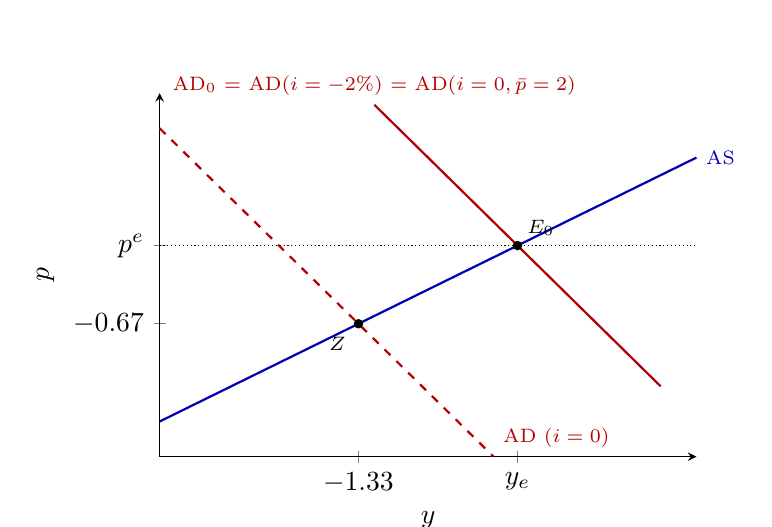
\begin{tikzpicture}
\begin{axis}[width=8.4cm,height=6.2cm,axis lines=left,xmin=-3,xmax=1.5,ymin=-1.8,ymax=1.3,clip=false,
  xlabel={$y$},ylabel={$p$},
  xtick={-1.3333,0},xticklabels={$-1.33$,$y_e$},ytick={-0.6667,0},yticklabels={$-0.67$,$p^e$}]
\addplot[densely dotted,domain=-3:1.5]{0};
\addplot[thick,blue!70!black,domain=-3:1.5]{0.5*x};
\addplot[thick,red!70!black,domain=-1.2:1.2]{-x};
\addplot[thick,red!70!black,dashed,domain=-3:-0.2]{-2-x};
\addplot[only marks,mark=*,mark size=1.5pt] coordinates {(0,0) (-1.3333,-0.6667)};
\node[font=\scriptsize,blue!70!black,anchor=west] at (axis cs:1.5,0.75) {AS};
\node[font=\scriptsize,red!70!black,anchor=south] at (axis cs:-1.2,1.2) {AD$_0$ $=$ AD($i=-2\%$) $=$ AD($i=0,\bar p=2$)};
\node[font=\scriptsize,red!70!black,anchor=south west] at (axis cs:-0.2,-1.8) {AD ($i=0$)};
\node[font=\scriptsize,anchor=north east] at (axis cs:-1.36,-0.70) {$Z$};
\node[font=\scriptsize,anchor=south west] at (axis cs:0,0) {$E_0$};
\end{axis}
\end{tikzpicture}\\
{\footnotesize The fall in $\bar y_n$ shifts AD left by 4; at $i=0$ it can only be brought back by 2, so the economy
sits at $Z$. Either $i=-2\%$ (infeasible) or $\bar p=2\%$ (a promise) puts AD back through $E_0$.}
\end{center}
\intuicao{Expecting to be poorer later, households cut consumption now. Only a negative real rate would persuade
them to spend; with $i$ stuck at zero, that negative real rate has to come from expected inflation.}
\refbib{Benigno (2015), \S9 (liquidity trap), Figs.~11--12, pp.~516--518; natural rate from \S5.}
\rubrica{
\item $r_n=-2\%$ derived and the desired $i$: 0.15. Calling it a supply shock or a trade-off: max.\ 0.2 on the item.
\item ZLB equilibrium $y=-1.33$, $p=-0.67$, gaps: 0.2 (slip: $-0.1$).
\item $\bar p=2\%$ and the real-rate mechanism, credibility: 0.2.
\item Graph: AS, AD shifted left, the partial return at $i=0$, point $Z$: 0.15.
}
\end{sol}

\parte{d}{0.9 point} Instead of a promise, the government raises current spending $g$ ($\bar g$ unchanged) while
$i$ stays at 0. Derive the multipliers $dy/dg$ and $d(y-y_e)/dg$, evaluate them, find the $g$ that closes the gap,
and check what happens to $p$. Then suppose the Copom were away from the ZLB and followed its optimal rule: what
would $dy/dg$ be? Explain why the ZLB makes fiscal policy more powerful here. Does Benigno's \S10 suggest even larger
multipliers? Show the effect of $g$ on the graph.
\resolespaco
\begin{sol}
\begin{notacao}
\item Symbols of (a)--(c) keep their meaning. New here:
\item $g\ge0$: current government spending, in percent of GDP; $\bar g=0$ unchanged.
\item $\omega\equiv\dfrac{\sigma^{-1}}{\sigma^{-1}+\eta}\in(0,1)$: response of $y_n$ and $y_e$ to $g$.
\item $dy/dg$: output multiplier. $d(y-y_e)/dg$: gap multiplier. $F$: the outcome with $g=4$.
\end{notacao}
\passo{1 --- $g$ moves both curves}{AD \eqref{q4:AD}: $+g$ one-for-one. AS: differentiate \eqref{q4:YN} and
\eqref{q4:YE} with respect to $g$:
\begin{equation}
\frac{dy_n}{dg}=\frac{dy_e}{dg}=\omega=\tfrac12, \label{q4d:omega}
\end{equation}
the wealth effect of taxes-to-come on labour supply. $y_n$ and $y_e$ rise by the same $\omega g$, so $g$ is not a
mark-up shock.}
\passo{2 --- solve}{Put $i=0$, $\bar p=0$, $\bar g=0$ in \eqref{q4:AD}:
\begin{align}
y &= \bar y_n+(g-0)-\sigma\big[(0)-(0-p)-\rho\big]\nonumber\\
&= \bar y_n+\sigma\rho+g-\sigma p. \label{q4d:ad}
\end{align}
AS \eqref{q4:AS} with $p^e=0$ and $y_n=\omega g$ from \eqref{q4d:omega}:
\begin{align}
p-(0) &= \kappa\big(y-(\omega g)\big)\nonumber\\
p &= \kappa(y-\omega g). \label{q4d:as}
\end{align}
Substitute \eqref{q4d:as} into \eqref{q4d:ad}:
\begin{align*}
y &= \bar y_n+\sigma\rho+g-\sigma\big(\kappa(y-\omega g)\big)\\
&= \bar y_n+\sigma\rho+g-\sigma\kappa y+\sigma\kappa\omega g\\
y(1+\sigma\kappa) &= \bar y_n+\sigma\rho+g(1+\sigma\kappa\omega).
\end{align*}
Differentiate with respect to $g$:
\begin{equation}
\boxed{\frac{dy}{dg}=\frac{1+\sigma\kappa\,\omega}{1+\sigma\kappa}}
=\frac{1+1\cdot\frac12\cdot\frac12}{1+1\cdot\frac12}=\boxed{\tfrac56}.
\label{q4d:mult}
\end{equation}
Subtract \eqref{q4d:omega} from \eqref{q4d:mult}:
\begin{align}
\frac{d(y-y_e)}{dg} &= \frac{1+\sigma\kappa\omega}{1+\sigma\kappa}-\omega\nonumber\\
&= \frac{1+\sigma\kappa\omega-\omega-\sigma\kappa\omega}{1+\sigma\kappa}\nonumber\\
&= \boxed{\frac{1-\omega}{1+\sigma\kappa}}=\frac{1-\frac12}{1+1\cdot\frac12}=\boxed{\tfrac13}. \label{q4d:gap}
\end{align}
These are Benigno's Table~1 $m_g=\frac{1}{1+\sigma\kappa}+\frac{\kappa}{(\sigma^{-1}+\eta)(1+\sigma\kappa)}$ and
$m_{\bar g}=\frac{\eta}{(\sigma^{-1}+\eta)(1+\sigma\kappa)}$ (with $\sigma\kappa\omega=\kappa/(\sigma^{-1}+\eta)$ and
$1-\omega=\eta/(\sigma^{-1}+\eta)$).}
\passo{3 --- closing the gap}{The gap at $Z$ is $-\tfrac43$ (part (c)). Divide by \eqref{q4d:gap}:
\[
g=\frac{4/3}{1/3}=\boxed{4\%}\ \text{of GDP}.
\]
Then, by \eqref{q4d:mult}, \eqref{q4d:omega} and \eqref{q4d:as}:
\begin{align*}
y &= -\tfrac43+\tfrac56\cdot4=\boxed{2},\\
y_n &= y_e=\omega g=\tfrac12\cdot4=2,\\
p &= \kappa(y-y_n)=\tfrac12(2-2)=\boxed{0=p^e}:
\end{align*}
both gaps closed, zero loss.}
\passo{4 --- away from the ZLB}{By \eqref{q4d:omega} spending moves $y_n$ and $y_e$ together, so there is no
trade-off: the optimal Copom satisfies \eqref{q4a:rule} with both gaps zero, $y=y_e(g)=\omega g$, $p=p^e$, raising
$i$ by $(1-\omega)g/\sigma$ to offset the excess demand in \eqref{q4:AD}. Then
$\boxed{dy/dg=\omega=\tfrac12}$.}
\passo{5 --- why larger at the ZLB}{Compare \eqref{q4d:mult} with $\omega$:
\[
\frac{1+\sigma\kappa\omega}{1+\sigma\kappa}>\omega\iff1>\omega\iff\eta>0.
\]
At the ZLB the Copom does not raise $i$ (it would like a \emph{lower} rate), so there is no crowding out through
the policy rate; only the price channel (a higher $p$ with $\bar p$ given raises the real rate) remains, which
keeps the multiplier below 1. In \S10 (Eggertsson--Krugman deleveraging) some households are
borrowing-constrained and spend every extra real of income, and falling prices raise real debt burdens: there the
multiplier at the ZLB can be much larger. With one representative household, as here, it stays at $5/6$.}
\begin{center}
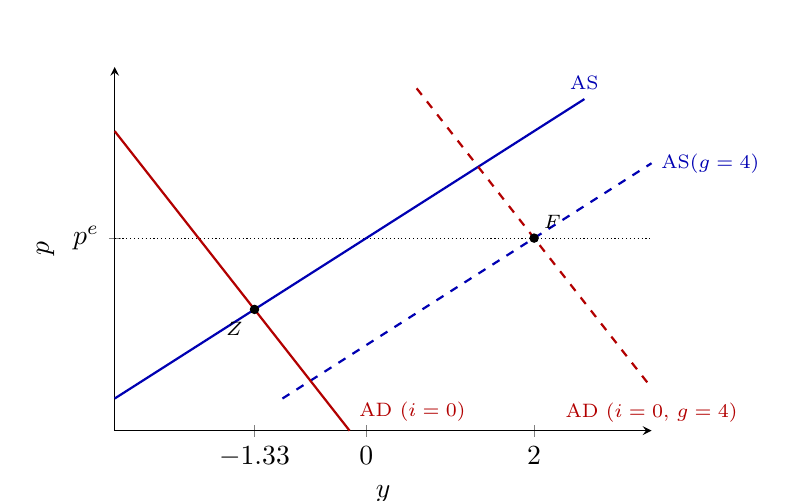
\begin{tikzpicture}
\begin{axis}[width=8.4cm,height=6.2cm,axis lines=left,xmin=-3,xmax=3.4,ymin=-1.8,ymax=1.6,clip=false,
  xlabel={$y$},ylabel={$p$},
  xtick={-1.3333,0,2},xticklabels={$-1.33$,$0$,$2$},ytick={0},yticklabels={$p^e$}]
\addplot[densely dotted,domain=-3:3.4]{0};
\addplot[thick,blue!70!black,domain=-3:2.6]{0.5*x};
\addplot[thick,blue!70!black,dashed,domain=-1:3.4]{0.5*(x-2)};
\addplot[thick,red!70!black,domain=-3:-0.2]{-2-x};
\addplot[thick,red!70!black,dashed,domain=0.6:3.4]{2-x};
\addplot[only marks,mark=*,mark size=1.5pt] coordinates {(-1.3333,-0.6667) (2,0)};
\node[font=\scriptsize,blue!70!black,anchor=south] at (axis cs:2.6,1.3) {AS};
\node[font=\scriptsize,blue!70!black,anchor=west] at (axis cs:3.4,0.7) {AS($g=4$)};
\node[font=\scriptsize,red!70!black,anchor=south west] at (axis cs:-0.2,-1.8) {AD ($i=0$)};
\node[font=\scriptsize,red!70!black,anchor=north] at (axis cs:3.4,-1.45) {AD ($i=0$, $g=4$)};
\node[font=\scriptsize,anchor=north east] at (axis cs:-1.36,-0.70) {$Z$};
\node[font=\scriptsize,anchor=south west] at (axis cs:2,0) {$F$};
\end{axis}
\end{tikzpicture}\\
{\footnotesize $g=4$ shifts AD right by 4 and AS right by $\omega g=2$; the new point $F=(2,\,p^e)$ has
$y=y_n=y_e$.}
\end{center}
\intuicao{Government spending adds demand directly and, by making households work more, adds supply too. When the
central bank is free it leans against the extra demand; stuck at zero it cannot, so more of the spending turns into
output.}
\refbib{Benigno (2015), \S8, eqs.~(22)--(23), Tables~1--2, pp.~514--516; \S9--\S10, pp.~516--521.}
\rubrica{
\item $g$ shifts AD and AS, with $\omega$: 0.15. Moving only AD: $-0.1$.
\item $dy/dg=5/6$ and $d(y-y_e)/dg=1/3$ derived: 0.25 (slip: $-0.1$). Reporting only the output multiplier: max.\ 0.15
on this line.
\item $g=4$ with $y=2$, $p=p^e$: 0.15.
\item Optimal-policy multiplier $\omega=1/2$ with the reason: 0.15.
\item Why larger at the ZLB and the \S10 remark: 0.1. Graph: 0.1.
}
\gap{Prova 01, Q3: which bar moves which curve, the sign of policy, and optimal policy as minimising the loss along AS;
here with a mark-up shock, where $\phi$ does matter, plus the ZLB and fiscal multipliers.}
\end{sol}

\ifsolucoes\else
\vfill
\begin{center}\footnotesize\textit{End of exam.}\end{center}
\fi

\end{document}
"   (run twice)
% Check fonts: pdffonts <file>.pdf  (all Type 1).
% Every number and closed form in the key: python simulado_codigo/check_simulado_05.py
% =============================================================================
\documentclass[11pt,a4paper]{article}
\usepackage[utf8]{inputenc}
\usepackage[T1]{fontenc}
\usepackage{lmodern}   % Type 1 vector fonts (replaces PK bitmaps)
\usepackage{cmap}      % ToUnicode CMap -> copyable text and accents
\usepackage[english]{babel}
\usepackage{amsmath,amssymb,amsfonts}
\usepackage[a4paper,margin=2.2cm]{geometry}
\usepackage{enumitem}
\usepackage{fancyhdr}
\usepackage{comment}
\usepackage{xcolor}
\usepackage{microtype}
\usepackage{booktabs}
\usepackage{needspace}
\usepackage{pgfplots}
\pgfplotsset{compat=1.18}
\usetikzlibrary{arrows.meta}

% ====================== CONFIGURATION ======================
\newif\ifsolucoes
\ifdefined\withsolutions\solucoestrue\else\solucoesfalse\fi

\newcommand{\disciplina}{Macroeconomics I --- MPE Insper}
\newcommand{\listatema}{Mock Exam 5}
\newcommand{\espacoresol}{6cm}

% ====================== MACHINERY ======================
\def\DefaultCutFileName{\def\CommentCutFile{\jobname.cut}}  % per-job cut file: parallel builds in Simulados/ would share comment.cut
\ifsolucoes\includecomment{sol}\else\excludecomment{sol}\fi

\pagestyle{fancy}\fancyhf{}
\lhead{\footnotesize\disciplina}
\rhead{\footnotesize \listatema\ifsolucoes{} --- Solutions and Rubric\fi}
\cfoot{\footnotesize\thepage}
\renewcommand{\headrulewidth}{0.3pt}
\setlength{\headheight}{14pt}

\setlist{topsep=2pt,itemsep=2pt}
\newcounter{questao}

\newcommand{\questao}[1]{\Needspace{12\baselineskip}\refstepcounter{questao}\bigskip\noindent
  {\large\bfseries\color{blue!55!black}Question \thequestao.}~#1\par\smallskip}
\newcommand{\parte}[2]{\par\Needspace{6\baselineskip}\medskip\noindent\textbf{#1)}~(#2)~}
\newcommand{\resolespaco}{\ifsolucoes\else\par\textit{Solution:}\vspace{\espacoresol}\par\fi}
\newcommand{\passo}[2]{\par\smallskip\noindent\textbf{Step #1.}~#2}
\newcommand{\intuicao}[1]{\par\smallskip\noindent\textit{Intuition.}~#1}
\newcommand{\refbib}[1]{\par\smallskip\noindent{\footnotesize\color{black!60}\textbf{Ref:} #1}}
\newcommand{\gap}[1]{\par\smallskip\noindent{\footnotesize\color{red!55!black}\textbf{Gap targeted:} #1}}
\newcommand{\trap}[1]{\par\smallskip\noindent{\small\color{red!55!black}\#~#1}}
\newcommand{\rubrica}[1]{\par\needspace{4\baselineskip}\smallskip\noindent\textbf{Grading rubric.}\begin{itemize}[leftmargin=1.4em,topsep=1pt]#1\end{itemize}}
\newenvironment{notacao}{\par\smallskip\noindent\textbf{Notation.}\begin{itemize}[leftmargin=1.4em,topsep=1pt,itemsep=0pt]\small}{\end{itemize}}
\allowdisplaybreaks
% Equation numbering: statement equations carry letter tags, (S1)-(S2), (U), (F), (BC), (AD), (AS), (YN),
% (YE), (LF), identical in both builds; solution equations are numbered (1), (2), ... and exist only in the
% solutions build. Labels are prefixed by item (q2b:...); statement text never cites a solution label.

% =============================================================================
\begin{document}
\begin{center}
  {\Large\bfseries \disciplina}\\[2pt]
  {\large \listatema\ (Simulado 5) --- whole course --- 2026, 3rd term}\ifsolucoes\\[2pt]\textit{Solutions and Grading Rubric}\fi
\end{center}
\vspace{2pt}

{\footnotesize\noindent\textbf{Instructions.} Four questions, 10 points in total. Duration: 3 hours, closed
book, non-programmable calculator allowed. Show every step; box final answers; sign every derivative before
interpreting it; in diagrams label the axes, name every curve and mark the direction of every shift.
Notation: Kurlat (2020) in Questions 1--3, Benigno (2015) in Question 4. All numbers are illustrative.
Natural logarithms throughout.\par}

\ifsolucoes
\medskip
{\footnotesize\noindent\textbf{How the rubric works.} Conceptual caps (``max.\ $x$'') bound an item whatever
else is right. Light penalties ($-0.1$) apply to arithmetic slips with a correct method. Caps and penalties
are \emph{not cumulative}: when a cap applies, the penalties inside it are ignored. Each question ends with the
weak spot it retests (``Gap targeted''). Every number and closed form below is recomputed by
\texttt{simulado\_codigo/check\_simulado\_05.py}.\par}
\fi

% =============================================================================
\questao{(2.0 points) Coffee, schools and saving in Minas Gerais.}

\noindent\textbf{Part A --- measurement.} One year in a coffee region, values in R\$ million.
\begin{itemize}[leftmargin=1.4em]
\item A trading company imports fertiliser for 50 and sells all of it to a coffee farm for 80. It pays 10 in wages.
\item The farm harvests coffee worth 300 at market prices. It sells 200 to a roaster, exports 60 to Germany, and
the remaining 40 is still in its warehouse, unsold, at the end of the year. It pays 120 in wages.
\item The roaster also imports packaging for 20 and sells all its roasted coffee, 450, to Brazilian households.
It pays 150 in wages.
\item The state government runs free public schools: it pays teachers 100 and buys nothing else.
\end{itemize}
Each firm's profit is whatever remains of its revenue after inputs and wages.

\parte{a}{1.0 point} (i) Compute the region's GDP by the product (value-added), income and expenditure
approaches, and show that they agree. (ii) Next year the farm harvests nothing. It sells its 40 of stored coffee
to the roaster, which roasts it and sells it to households for 90; nothing else happens in this chain. Compute
the chain's contribution to next year's GDP by the product and the expenditure approaches. (iii) A columnist
writes: ``This year's GDP overstates the region's output, because 40 of coffee was never sold; and it understates
it, because the schools charge nothing.'' Evaluate each half of the claim.
\resolespaco
\begin{sol}
\begin{notacao}
\item Trader, farm, roaster, government: the four producers; $j$ indexes them. All values in R\$ million.
\item $VA_j\ge0$: value added of producer $j$, its gross output minus the intermediate inputs it uses up
(imported inputs included).
\item $\text{wages}_j\ge0$, $\text{profit}_j$: payments to workers and the operating surplus left to owners.
\item $C$, $I$, $G$, $X$, $M$: household consumption, investment (fixed capital plus change in inventories,
so $I$ can be negative), government purchases, exports and imports, all $\ge0$ except $I$.
\end{notacao}
\passo{0 --- the definitions used below}{GDP is the market value of final goods and services produced in the
region in the year. The three approaches:
\begin{align}
VA_j &= \text{gross output}_j-\text{intermediate inputs}_j, \label{q1a:va}\\
\text{GDP} &= \textstyle\sum_j VA_j, \label{q1a:prod}\\
\text{profit}_j &= VA_j-\text{wages}_j, \label{q1a:profit}\\
\text{GDP} &= \textstyle\sum_j(\text{wages}_j+\text{profit}_j), \label{q1a:inc}\\
\text{GDP} &= C+I+G+X-M. \label{q1a:exp}
\end{align}
Non-market output (public schools) has no price, so its gross output is valued \emph{at cost}.}
\passo{1 --- value added (product)}{Apply \eqref{q1a:va} to each producer. The farm's output is the whole
harvest, sold or not; the government's is its cost:
\begin{align*}
VA_{\text{trader}} &= 80-50=30,\\
VA_{\text{farm}} &= 300-80=220,\\
VA_{\text{roaster}} &= 450-200-20=230,\\
VA_{\text{gov}} &= 100.
\end{align*}
Sum with \eqref{q1a:prod}:
\[
\text{GDP}=30+220+230+100=\boxed{580}.
\]}
\passo{2 --- income}{Wages paid by the four producers:
\[
10+120+150+100=380.
\]
Profits from \eqref{q1a:profit}, using the value added of Step 1:
\begin{align*}
\text{profit}_{\text{trader}} &= 30-10=20,\\
\text{profit}_{\text{farm}} &= 220-120=100\quad\text{(it includes the 40 of stock, at market price)},\\
\text{profit}_{\text{roaster}} &= 230-150=80,\\
\text{profit}_{\text{gov}} &= 100-100=0\quad\text{(valued at cost, so no surplus)}.
\end{align*}
Sum with \eqref{q1a:inc}:
\[
\text{GDP}=380+20+100+80=\boxed{580}.
\]}
\passo{3 --- expenditure}{Final uses: households buy the roasted coffee, $C=450$; the unsold coffee is output
kept by its producer, \emph{inventory investment} $I=40$; $G=100$; $X=60$. Imports:
\[
M=50+20=70.
\]
Substitute into \eqref{q1a:exp}:
\[
\text{GDP}=450+40+100+60-70=\boxed{580}.
\]}
\begin{center}\small
\begin{tabular}{@{}lccccc@{}}
\toprule
Approach & Trader & Farm & Roaster & Government & GDP\\
\midrule
Product (VA) & 30 & 220 & 230 & 100 & \textbf{580}\\
Income (wages $+$ profit) & $10+20$ & $120+100$ & $150+80$ & $100+0$ & \textbf{580}\\
Expenditure & \multicolumn{4}{c}{$C=450,\ I=40,\ G=100,\ X=60,\ M=-70$} & \textbf{580}\\
\bottomrule
\end{tabular}
\end{center}
\passo{4 --- next year}{Product, by \eqref{q1a:va}: the farm produces nothing new (selling an old stock is not
production), so $VA_{\text{farm}}=0$, and
\[
VA_{\text{roaster}}=90-40=\boxed{50}.
\]
Expenditure, by \eqref{q1a:exp}: $C=+90$, and inventories fall, $I=-40$:
\[
\text{GDP}_{\text{chain}}=90-40=\boxed{50}.
\]
The 40 was counted last year as investment; counting it again as consumption would double-count it, so the
inventory drawdown enters as \emph{negative} investment.}
\passo{5 --- the columnist}{First half: \textbf{wrong}. GDP measures production, not sales; the 40 was
produced this year and \eqref{q1a:exp} records it as investment in inventories. Second half:
\textbf{wrong as stated}. The schools are in GDP, valued at the cost of the teachers (100), even with a zero
price. What GDP may miss is any value of the service above its cost --- a ``beyond GDP'' issue, not an omission.
Contrast with Prova 01: a free online service paid by advertising enters only through the ad revenue, which is
an intermediate input of the advertiser.}
\intuicao{Every real a firm earns is either a payment to a factor or a purchase from another firm; summing value
added nets out the purchases. Imports are subtracted because they are someone else's production; stocks are
added because they are this year's production that nobody bought yet.}
\refbib{Kurlat ch.~1, \S1.1, pp.~15--21: inventories p.~18; government output at cost, Example~1.7, p.~20.}
\rubrica{
\item (i) Each approach with its own entries: 0.2 each (0.6). Treating the 40 as not produced, or leaving
imports in VA: max.\ 0.3 on (i). Putting the teachers into $C$ instead of $G$: $-0.1$.
\item (ii) 50 by both approaches, with $I=-40$: 0.2. Adding the 40 again (GDP 90): 0 on (ii).
\item (iii) Both halves, each with its reason: 0.2.
}
\end{sol}

\medskip
\noindent\textbf{Part B --- saving and growth.} The Ministry of Planning uses the Solow model in
\emph{per-worker} terms, with no technological progress, saving rate $s$, population growth $n$
and depreciation $\delta$ constant:
\begin{align}
y &= Ak^{\alpha}, \tag{S1}\label{q1:prod}\\
(1+n)k_{t+1} &= (1-\delta)k_t+sAk_t^{\alpha}. \tag{S2}\label{q1:lom}
\end{align}
Brazil is in steady state with $\alpha=1/3$ and $s=0.15$.

\parte{b}{1.0 point} (i) Derive steady-state capital $k^{*}$ and consumption $c^{*}$ per worker as functions of
$s$, and find the saving rate $s_{GR}$ that maximises $c^{*}$. Confirm it with a condition on the marginal
product of capital. (ii) A pension reform raises the saving rate permanently from $0.15$ to $s_{GR}$ at date
$t_0$. Compute the percentage change in consumption per worker on impact and between the two steady states,
and the change in steady-state output per worker. (iii) Show graphically: the Solow diagram before and after
the reform, and the time paths of $y$ and $c$. (iv) Is the reform necessarily good for Brazilians? Who pays for
it?
\resolespaco
\begin{sol}
\begin{notacao}
\item $y_t$, $k_t$, $c_t>0$: output, capital and consumption per worker at date $t$.
\item $A>0$: total factor productivity, constant. $\alpha\in(0,1)$: capital's income share ($\alpha=1/3$).
\item $s\in(0,1)$: saving rate. $n\ge0$: population growth. $\delta\in(0,1)$: depreciation rate.
\item $k^*$, $y^*$, $c^*$: steady-state values. $s_{GR}$: the golden-rule saving rate.
\item $t_0$: date of the reform; ``old'' and ``new'' index the steady states at $s=0.15$ and $s=s_{GR}$.
\end{notacao}
\passo{1 --- steady state}{Set $k_{t+1}=k_t=k^*$ in \eqref{q1:lom}:
\begin{align}
(1+n)k^* &= (1-\delta)k^*+sA(k^*)^{\alpha}\nonumber\\
(n+\delta)k^* &= sA(k^*)^{\alpha}\nonumber\\
(k^*)^{1-\alpha} &= \frac{sA}{n+\delta}. \nonumber
\end{align}
Raise both sides to the power $1/(1-\alpha)$:
\begin{equation}
\boxed{k^*=\left(\frac{sA}{n+\delta}\right)^{\frac{1}{1-\alpha}}} \label{q1b:kss}
\end{equation}
Consumption is the part of output not saved:
\begin{equation}
c=(1-s)\,y. \label{q1b:c}
\end{equation}
Evaluate \eqref{q1:prod} at \eqref{q1b:kss}:
\begin{align}
y^* &= A(k^*)^{\alpha}\nonumber\\
&= A\left[\left(\frac{sA}{n+\delta}\right)^{\frac{1}{1-\alpha}}\right]^{\alpha}\nonumber\\
&= A\left(\frac{sA}{n+\delta}\right)^{\frac{\alpha}{1-\alpha}}. \label{q1b:yss}
\end{align}
Substitute \eqref{q1b:yss} into \eqref{q1b:c}:
\begin{align}
c^* &= (1-s)\left[A\left(\frac{sA}{n+\delta}\right)^{\frac{\alpha}{1-\alpha}}\right]\nonumber\\
&= \boxed{(1-s)A\left(\frac{sA}{n+\delta}\right)^{\frac{\alpha}{1-\alpha}}} \label{q1b:css}
\end{align}
\#~The exponent is $\alpha/(1-\alpha)$: $k^*$ is raised to $\alpha$ inside $f$.}
\passo{2 --- golden rule}{Take the log of \eqref{q1b:css}:
\begin{equation}
\ln c^*=\ln A+\ln(1-s)+\frac{\alpha}{1-\alpha}\Big[\ln s+\ln A-\ln(n+\delta)\Big]. \label{q1b:lnc}
\end{equation}
Differentiate \eqref{q1b:lnc} with respect to $s$ and set it to zero:
\begin{equation}
-\frac{1}{1-s}+\frac{\alpha}{(1-\alpha)s}=0. \label{q1b:foc}
\end{equation}
Multiply \eqref{q1b:foc} by $(1-\alpha)s(1-s)>0$:
\begin{align*}
-(1-\alpha)s+\alpha(1-s) &= 0\\
\alpha-s &= 0.
\end{align*}
Hence
\begin{equation}
\boxed{s_{GR}=\alpha=\tfrac13}. \label{q1b:sgr}
\end{equation}
SOC: differentiating \eqref{q1b:foc} again gives $-\frac{1}{(1-s)^2}-\frac{\alpha}{(1-\alpha)s^2}<0$, a maximum.}
\passo{2b --- cross-check through $k$}{In a steady state, \eqref{q1:lom} with $k_{t+1}=k_t=k$ gives
\begin{equation}
sAk^{\alpha}=(n+\delta)\,k. \label{q1b:ss}
\end{equation}
Substitute \eqref{q1:prod} into \eqref{q1b:c}, then use \eqref{q1b:ss}:
\begin{align}
c &= (1-s)\big(Ak^{\alpha}\big)\nonumber\\
&= Ak^{\alpha}-sAk^{\alpha}\nonumber\\
&= Ak^{\alpha}-\big((n+\delta)k\big)\nonumber\\
&= Ak^{\alpha}-(n+\delta)k. \label{q1b:ck}
\end{align}
Set the derivative of \eqref{q1b:ck} with respect to $k$ to zero:
\begin{equation}
\boxed{\alpha Ak^{\alpha-1}=n+\delta}\qquad(\text{MPK}=n+\delta). \label{q1b:mpk}
\end{equation}
Solve \eqref{q1b:ss} for $s$ and substitute \eqref{q1b:mpk} for $n+\delta$:
\begin{align*}
s &= \frac{(n+\delta)k}{Ak^{\alpha}}\\
&= \frac{\big(\alpha Ak^{\alpha-1}\big)\,k}{Ak^{\alpha}}\\
&= \alpha\ \checkmark
\end{align*}
Knife edge: $\alpha\to0\Rightarrow s_{GR}\to0$ (capital useless, save nothing). The Prova~01 slip (exponent
$1/(1-\alpha)$ instead of $\alpha/(1-\alpha)$) gives $s=1/(2-\alpha)=0.6$ here, which fails this test.}
\passo{3 --- impact}{At $t_0$ capital is predetermined, so $y$ does not move and, by \eqref{q1b:c}, only the
factor $1-s$ changes:
\begin{align*}
\frac{c_{t_0}}{c_{\text{old}}} &= \frac{(1-s_{GR})\,y^*_{\text{old}}}{(1-0.15)\,y^*_{\text{old}}}\\
&= \frac{1-1/3}{1-0.15}\\
&= \frac{0.6667}{0.85}\\
&= 0.7843,
\end{align*}
a fall of $\boxed{21.6\%}$.}
\passo{4 --- long run}{Divide \eqref{q1b:css} at $s_{GR}$ by \eqref{q1b:css} at $0.15$; $A$, $n$ and $\delta$ cancel,
and $(1/3)/0.15=2.2222$, $\alpha/(1-\alpha)=1/2$:
\begin{align*}
\frac{c^*_{\text{new}}}{c^*_{\text{old}}} &= \frac{(1-1/3)A\left(\frac{(1/3)A}{n+\delta}\right)^{\frac{1/3}{2/3}}}
{(1-0.15)A\left(\frac{0.15A}{n+\delta}\right)^{\frac{1/3}{2/3}}}\\
&= \frac{1-1/3}{1-0.15}\left(\frac{1/3}{0.15}\right)^{\frac{1/3}{2/3}}\\
&= 0.7843\times(2.2222)^{1/2}\\
&= 0.7843\times1.4907\\
&= 1.1692,
\end{align*}
a rise of $\boxed{16.9\%}$. Output, from the ratio of \eqref{q1b:yss}:
\begin{align*}
\frac{y^*_{\text{new}}}{y^*_{\text{old}}} &= \frac{A\left(\frac{(1/3)A}{n+\delta}\right)^{1/2}}{A\left(\frac{0.15A}{n+\delta}\right)^{1/2}}\\
&= (2.2222)^{1/2}=1.4907,\quad\boxed{+49.1\%}.
\end{align*}
Capital, from the ratio of \eqref{q1b:kss} (exponent $1/(1-\alpha)=3/2$): $(2.2222)^{3/2}=3.313$.}
\passo{5 --- graphs}{Left: $sAk^{\alpha}$ rotates up, and the crossing with $(n+\delta)k$, \eqref{q1b:ss}, moves
from $k^*_{\text{old}}$ to $k^*_{GR}$; arrows along the $k$ axis point right in between. Right: $y$ starts at its
old level and rises monotonically (no jump, $k$ is a stock); $c$ jumps down at $t_0$, then rises, overtakes its
old level and converges to a level 16.9\% higher. The curves are simulated from \eqref{q1:lom} with $A=1$,
$n=1\%$, $\delta=5\%$ a year; with these values $c$ regains its old level after 18 years.}
\begin{center}
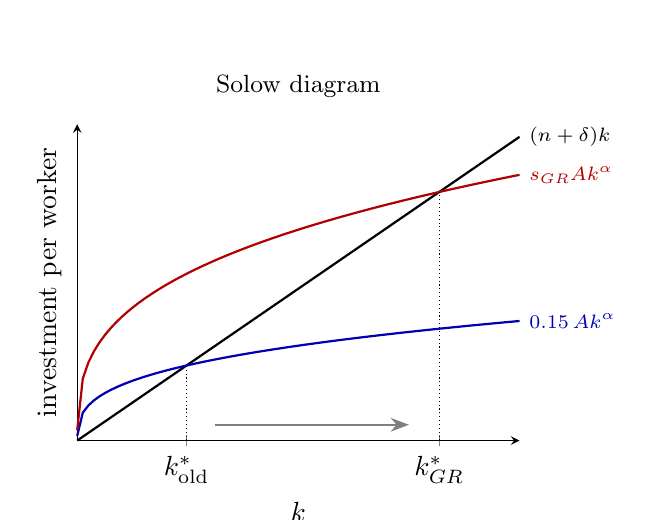
\begin{tikzpicture}
\begin{axis}[width=7.2cm,height=5.6cm,axis lines=left,xmin=0,xmax=16,ymin=0,ymax=1.0,
  xlabel={$k$},ylabel={investment per worker},xtick={3.953,13.095},xticklabels={$k^*_{\text{old}}$,$k^*_{GR}$},
  ytick=\empty,title={\small Solow diagram},clip=false]
\addplot[thick,black,domain=0:16,samples=60]{0.06*x};
\addplot[thick,blue!70!black,domain=0.001:16,samples=80]{0.15*x^(1/3)};
\addplot[thick,red!70!black,domain=0.001:16,samples=80]{(1/3)*x^(1/3)};
\addplot[densely dotted] coordinates {(3.953,0) (3.953,0.2372)};
\addplot[densely dotted] coordinates {(13.095,0) (13.095,0.7857)};
\node[font=\scriptsize,anchor=west] at (axis cs:16,0.96) {$(n+\delta)k$};
\node[font=\scriptsize,blue!70!black,anchor=west] at (axis cs:16,0.378) {$0.15\,Ak^{\alpha}$};
\node[font=\scriptsize,red!70!black,anchor=west] at (axis cs:16,0.84) {$s_{GR}Ak^{\alpha}$};
\draw[-{Stealth},thick,gray] (axis cs:5,0.05)--(axis cs:12,0.05);
\end{axis}
\end{tikzpicture}\quad
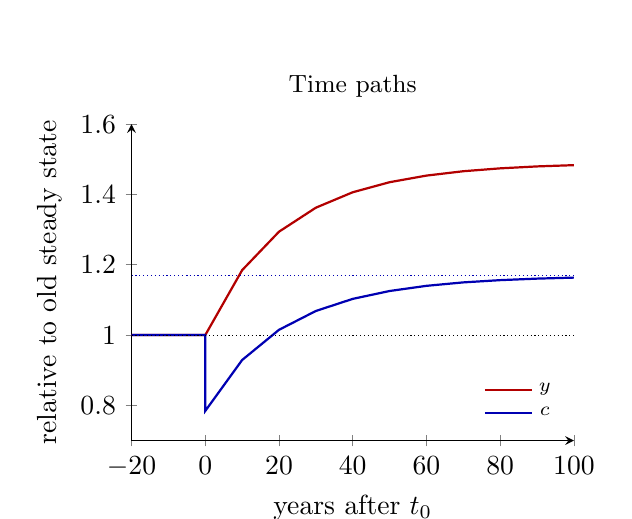
\begin{tikzpicture}
\begin{axis}[width=7.2cm,height=5.6cm,axis lines=left,xmin=-20,xmax=100,ymin=0.7,ymax=1.6,
  xlabel={years after $t_0$},ylabel={relative to old steady state},title={\small Time paths},
  legend style={font=\scriptsize,draw=none,at={(0.98,0.03)},anchor=south east}]
\addplot[thick,red!70!black] coordinates {(-20,1) (0,1) (10,1.1847) (20,1.2941) (30,1.3624) (40,1.4063)
  (50,1.4349) (60,1.4537) (70,1.4661) (80,1.4743) (90,1.4798) (100,1.4834)};
\addplot[thick,blue!70!black] coordinates {(-20,1) (0,1) (0,0.7843) (10,0.9291) (20,1.0150) (30,1.0686)
  (40,1.1030) (50,1.1254) (60,1.1401) (70,1.1499) (80,1.1563) (90,1.1606) (100,1.1635)};
\addplot[densely dotted,domain=-20:100]{1};
\addplot[densely dotted,blue!70!black,domain=-20:100]{1.1692};
\legend{$y$,$c$}
\end{axis}
\end{tikzpicture}
\end{center}
\passo{6 --- welfare}{Not necessarily. Brazil starts \emph{below} the golden rule ($0.15<1/3$), so the economy
is dynamically efficient and more steady-state consumption must be bought with less consumption during the
transition: current workers and retirees pay (21.6\% less consumption at once, below the old level for 18
years); later cohorts gain. Whether it is worth it depends on how the future is discounted --- an impatient
society optimally stays below $s_{GR}$ (compare optimal and fixed saving rates, Kurlat ex.~9.12, p.~185).
Only from \emph{above} $s_{GR}$ would a change (a cut in $s$) raise consumption at every date, a Pareto
improvement.}
\intuicao{A higher saving rate keeps raising output, but each extra unit of capital also needs $n+\delta$ of
replacement; past the point where MPK $=n+\delta$, capital costs more to maintain than it adds. With
Cobb--Douglas that point is reached exactly when the saving rate equals capital's income share.}
\refbib{Kurlat ch.~4, \S4.2 (steady state, pp.~59--61) and \S4.3 (golden rule, pp.~61--63); Jones (2020) ch.~5
for the transition paths.}
\rubrica{
\item (i) $k^*$ and $c^*$ with the exponent $\alpha/(1-\alpha)$: 0.15; $s_{GR}=\alpha$ derived: 0.1; MPK
cross-check: 0.1. Dropping the exponent (answer other than $\alpha$): max.\ 0.15 on (i). Maximising $k^*$ or
$y^*$ instead of $c^*$: 0 on (i).
\item (ii) Impact $-21.6\%$ with the reason (predetermined $k$): 0.1; $+16.9\%$ and $+49.1\%$: 0.15 (slip:
$-0.1$). Consumption rising on impact: 0 on that line.
\item (iii) Solow diagram with both curves and both crossings labelled: 0.1; time paths, $c$ jumping down and
$y$ not jumping: 0.1.
\item (iv) Trade-off and who pays: 0.1; why only above $s_{GR}$ is a change Pareto improving: 0.1.
}
\gap{Prova 01, 1.b--1.c (three approaches with all entries; what counts as investment) and 2.b (golden-rule
algebra: carry the exponent, cross-check with MPK $=n+\delta$).}
\end{sol}

% =============================================================================
\questao{(2.5 points) A labour tax: what it does depends on what the government does with the money.
\textnormal{\normalsize A one-period economy has a fixed capital stock $\bar K$, owned by the representative
household, which also owns the competitive firm. The household has one unit of time and utility
\eqref{q2:U}, with $\psi=1/3$. The firm produces \eqref{q2:F} with $\alpha=1/3$;
normalise $A\bar K^{\alpha}=1$. Labour income is taxed at rate $\tau$, so the household's budget is
\eqref{q2:BC}, where $T$ is a lump-sum transfer that the household takes as given:
\begin{align}
u &= \ln c+\psi\ln(1-L), \tag{U}\label{q2:U}\\
Y &= A\bar K^{\alpha}L^{1-\alpha}, \tag{F}\label{q2:F}\\
c &= (1-\tau)wL+r\bar K+\Pi+T. \tag{BC}\label{q2:BC}
\end{align}
Congress debates a 25\% tax on labour income.}}

\parte{a}{0.7 point} Let $\tau=T=0$. Write the household's and the firm's problems, their first-order
conditions and the market-clearing conditions; show that profits are zero, and find the equilibrium $L$, $Y$,
$w$ and $c$. Then solve the problem of a planner who chooses $c$ and $L$ subject only to technology, and show that
it gives the same allocation. State the theorem behind this and the assumptions it needs.
\resolespaco
\begin{sol}
\begin{notacao}
\item $c\ge0$: consumption. $L\in[0,1]$: hours worked; $1-L$: leisure (one unit of time).
\item $\psi>0$: weight of leisure in utility ($\psi=1/3$).
\item $Y$: output. $\bar K>0$: fixed capital stock. $A>0$: productivity, with $A\bar K^{\alpha}=1$.
$\alpha\in(0,1)$: capital's share ($\alpha=1/3$).
\item $w$, $r>0$: real wage and real rental rate of capital. $\Pi$: the firm's profit, paid to the household.
\item $\tau\in[0,1)$: tax rate on labour income. $T$: lump-sum transfer. In this item $\tau=T=0$.
\item $L_0$, $Y_0$, $w_0$, $c_0$: the equilibrium at $\tau=0$. $L^{P}$: the planner's choice.
\item MRS: marginal rate of substitution of leisure for consumption. MPL: marginal product of labour.
\end{notacao}
\passo{1 --- household}{With $\tau=T=0$, \eqref{q2:BC} is
\begin{equation}
c=wL+r\bar K+\Pi. \label{q2a:bc}
\end{equation}
Substitute \eqref{q2a:bc} into \eqref{q2:U}:
\[
\max_L\ \ln(wL+r\bar K+\Pi)+\psi\ln(1-L).
\]
Differentiate with respect to $L$ and set it to zero:
\[
\frac{w}{c}-\frac{\psi}{1-L}=0.
\]
Rearrange:
\begin{equation}
\boxed{\frac{\psi c}{1-L}=w} \label{q2a:hh}
\end{equation}
--- the marginal rate of substitution between leisure and consumption equals the real wage, the price of
leisure.}
\passo{2 --- firm}{The firm chooses $L$ and rents $\bar K$:
$\max\ A\bar K^{\alpha}L^{1-\alpha}-wL-r\bar K$. Differentiating \eqref{q2:F}:
\begin{align}
w &= (1-\alpha)A\bar K^{\alpha}L^{-\alpha}\nonumber\\
&= \frac{(1-\alpha)\big(A\bar K^{\alpha}L^{1-\alpha}\big)}{L}\nonumber\\
&= \frac{(1-\alpha)Y}{L}, \label{q2a:w}\\
r &= \alpha A\bar K^{\alpha-1}L^{1-\alpha}\nonumber\\
&= \frac{\alpha\big(A\bar K^{\alpha}L^{1-\alpha}\big)}{\bar K}\nonumber\\
&= \frac{\alpha Y}{\bar K}. \label{q2a:r}
\end{align}
Profits, using \eqref{q2a:w} and \eqref{q2a:r}:
\begin{align}
\Pi &= Y-wL-r\bar K\nonumber\\
&= Y-\left(\frac{(1-\alpha)Y}{L}\right)L-\left(\frac{\alpha Y}{\bar K}\right)\bar K\nonumber\\
&= Y-(1-\alpha)Y-\alpha Y\nonumber\\
&= \boxed{0} \label{q2a:pi}
\end{align}
(constant returns: factor payments exhaust output).}
\passo{3 --- clearing}{Labour: household supply $=$ firm demand; capital: $\bar K$; goods (no $G$):
\begin{equation}
c=Y. \label{q2a:goods}
\end{equation}}
\passo{4 --- solve}{Substitute \eqref{q2a:goods} and \eqref{q2a:w} into \eqref{q2a:hh}:
\begin{align*}
\frac{\psi\,(Y)}{1-L} &= \left(\frac{(1-\alpha)Y}{L}\right)\\
\psi L &= (1-\alpha)(1-L)\\
(1-\alpha+\psi)L &= 1-\alpha.
\end{align*}
Hence
\begin{align}
L_0 &= \boxed{\frac{1-\alpha}{1-\alpha+\psi}}\nonumber\\
&= \frac{1-\frac13}{1-\frac13+\frac13}\nonumber\\
&= \frac{2/3}{1}=\boxed{\tfrac23}. \label{q2a:L0}
\end{align}
Then, by \eqref{q2:F} with $A\bar K^{\alpha}=1$, \eqref{q2a:w}, \eqref{q2a:goods} and \eqref{q2a:r}:
\begin{align*}
Y_0 &= (2/3)^{2/3}=0.7631,\\
w_0 &= \frac{(2/3)(0.7631)}{2/3}=0.7631,\\
c_0 &= Y_0=0.7631,\\
r\bar K &= \alpha Y_0=\tfrac13(0.7631)=0.2544.
\end{align*}}
\passo{5 --- planner}{The planner substitutes technology \eqref{q2:F} into \eqref{q2:U}:
\begin{align}
\max_L\ \ln\!\big(A\bar K^{\alpha}L^{1-\alpha}\big)+\psi\ln(1-L)
=\text{const}+(1-\alpha)\ln L+\psi\ln(1-L). \label{q2a:plan}
\end{align}
Differentiate \eqref{q2a:plan} with respect to $L$:
\begin{equation}
\frac{1-\alpha}{L}=\frac{\psi}{1-L}. \label{q2a:planfoc}
\end{equation}
Cross-multiplying \eqref{q2a:planfoc} gives the second line of Step 4, so $L^{P}=\tfrac23$ (SOC: both terms
concave). The planner sets MRS $=$ MPL; the market sets MRS $=w$ \eqref{q2a:hh} and MPL $=w$ \eqref{q2a:w},
hence MRS $=$ MPL.}
\passo{6 --- theorem}{\textbf{First Welfare Theorem}: a competitive equilibrium is Pareto efficient, given
price-taking agents, complete markets, no externalities and no distortionary taxes. Here all hold at $\tau=0$.}
\refbib{Kurlat ch.~9, \S9.1--\S9.2, pp.~165--172 (equilibrium and the First Welfare Theorem); ch.~7, \S7.2,
pp.~131--137 (consumption--leisure choice).}
\rubrica{
\item Household FOC (MRS $=w$) and firm FOCs: 0.2. $\Pi=0$ shown: 0.1. Clearing conditions listed: 0.1.
\item $L_0=2/3$ with $Y,w,c$: 0.1 (slip: $-0.1$).
\item Planner's FOC and same allocation: 0.1. Theorem and its assumptions: 0.1.
\item Omitting capital income or profits from the budget: max.\ 0.4 on the item.
}
\end{sol}

\parte{b}{0.7 point} Now $\tau=25\%$ and the government returns the whole revenue as the transfer, so
$T=\tau wL$ in equilibrium. Find $L$ (in general and in numbers). Explain why returning the money does not undo
the effect of the tax. Show graphically, in the plane (leisure $\ell=1-L$, consumption $c$): the production
possibilities frontier, the equilibrium of (a), the new equilibrium, and the household's budget line at the new
equilibrium, with and without the transfer. Use the graph to explain why the new allocation is inefficient.
\resolespaco
\begin{sol}
\begin{notacao}
\item Symbols of (a) keep their meaning. New here:
\item $\tau=0.25$; $T=\tau wL$: the rebate, equal to the revenue in equilibrium, taken as given by the household.
\item $L_R$: hours under the rebated tax. $\ell\equiv1-L\in[0,1]$: leisure; $\ell_0$, $\ell_R$ at the two equilibria.
\item $E_0$, $E_R$: the equilibria of (a) and (b). $U_0$, $U_R$: the indifference curves through them.
\end{notacao}
\passo{1 --- FOC with the tax}{Substitute \eqref{q2:BC} into \eqref{q2:U}:
\[
\max_L\ \ln\big((1-\tau)wL+r\bar K+\Pi+T\big)+\psi\ln(1-L).
\]
Differentiate with respect to $L$, with $T$ taken as given, and set it to zero:
\[
\frac{(1-\tau)w}{c}-\frac{\psi}{1-L}=0.
\]
Rearrange, as in (a), now with $(1-\tau)w$ per hour:
\begin{equation}
\boxed{\frac{\psi c}{1-L}=(1-\tau)w}. \label{q2b:hh}
\end{equation}
$T$ does not appear: the household takes it as given, so it moves income, not the price of leisure.}
\passo{2 --- equilibrium}{The government returns the revenue:
\begin{equation}
T=\tau wL. \label{q2b:gov}
\end{equation}
Substitute \eqref{q2b:gov} into \eqref{q2:BC}, with $\Pi=0$ from \eqref{q2a:pi}, and then use \eqref{q2a:w} and
\eqref{q2a:r}:
\begin{align}
c &= (1-\tau)wL+r\bar K+(0)+(\tau wL)\nonumber\\
&= wL+r\bar K\nonumber\\
&= \left(\frac{(1-\alpha)Y}{L}\right)L+\left(\frac{\alpha Y}{\bar K}\right)\bar K\nonumber\\
&= (1-\alpha)Y+\alpha Y\nonumber\\
&= Y. \label{q2b:cY}
\end{align}
Substitute \eqref{q2b:cY} and \eqref{q2a:w} into \eqref{q2b:hh}:
\begin{align*}
\frac{\psi\,(Y)}{1-L} &= (1-\tau)\left(\frac{(1-\alpha)Y}{L}\right)\\
\psi L &= (1-\tau)(1-\alpha)(1-L).
\end{align*}
Solve for $L$:
\begin{equation}
\boxed{L_R=\frac{(1-\tau)(1-\alpha)}{\psi+(1-\tau)(1-\alpha)}}. \label{q2b:LR}
\end{equation}
Numbers: $(1-\tau)(1-\alpha)=0.75\cdot\tfrac23=0.5$, so
\[
L_R=\frac{0.5}{\frac13+0.5}=\frac{0.5}{0.8333}=\boxed{0.60}.
\]
Sign, differentiating \eqref{q2b:LR}:
\[
\frac{\partial L_R}{\partial\tau}=-\frac{\psi(1-\alpha)}{[\psi+(1-\tau)(1-\alpha)]^2}<0.
\]
The other variables, by \eqref{q2:F}, \eqref{q2a:w}, \eqref{q2b:gov}, \eqref{q2a:r} and \eqref{q2b:cY}:
\begin{align*}
Y &= 0.6^{2/3}=0.7114,\\
w &= \frac{(2/3)(0.7114)}{0.6}=0.7904,\\
(1-\tau)w &= 0.75(0.7904)=0.5928,\\
T &= 0.25(0.7904)(0.6)=0.1186=\tau(1-\alpha)Y,\\
r\bar K &= \alpha Y=\tfrac13(0.7114)=0.2371,\\
c &= Y=0.7114.
\end{align*}}
\passo{3 --- why the rebate does not undo it}{Each household compares one more hour with $(1-\tau)w$, not
with $w$: its own extra hour raises the transfer to \emph{everyone} by a negligible amount, so it ignores it.
In equilibrium the transfer returns the \emph{income} (\eqref{q2b:cY}: $c=Y$ exactly) but the \emph{price} of
leisure stays distorted. Combining \eqref{q2b:hh} with $w=\text{MPL}$ from \eqref{q2a:w}:
\#~a wedge, $\text{MRS}=(1-\tau)\,\text{MPL}<\text{MPL}$.}
\begin{center}
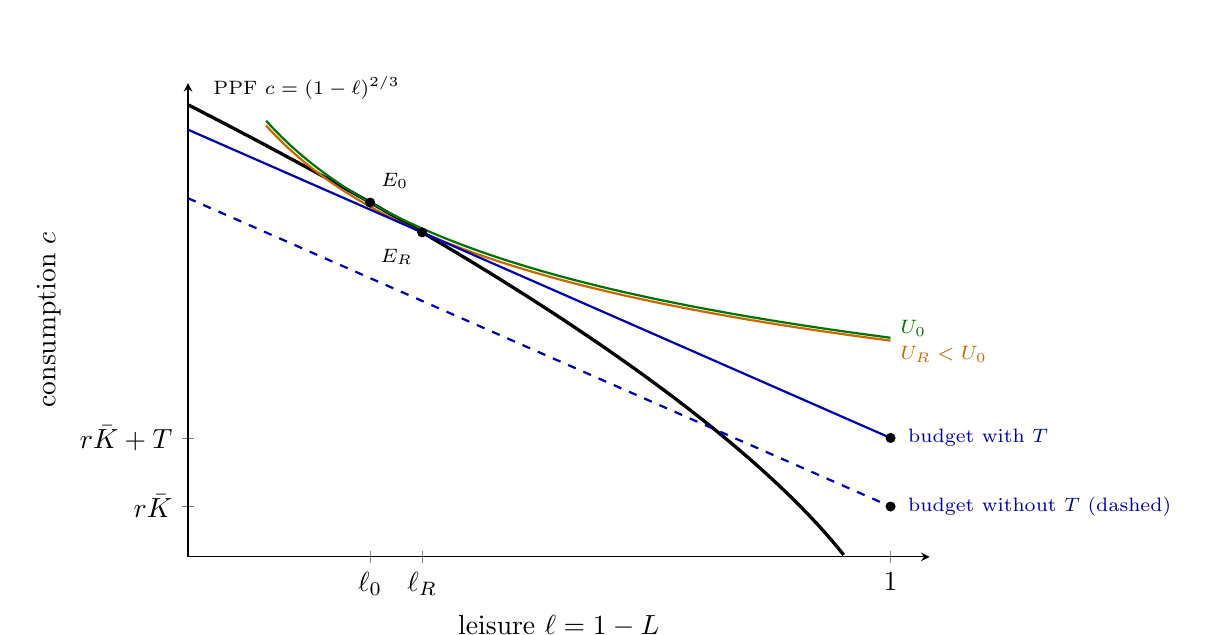
\begin{tikzpicture}
\begin{axis}[width=11cm,height=7.6cm,axis lines=left,xmin=0.1,xmax=1.05,ymin=0.15,ymax=0.97,clip=false,
  xlabel={leisure $\ell=1-L$},ylabel={consumption $c$},xtick={0.3333,0.4,1},xticklabels={$\ell_0$,$\ell_R$,$1$},
  ytick={0.2371,0.3557},yticklabels={$r\bar K$,$r\bar K+T$}]
\addplot[very thick,black,domain=0.1:0.94,samples=120]{(1-x)^(2/3)};
\addplot[thick,green!45!black,domain=0.2:1,samples=80]{0.52912*x^(-1/3)};
\addplot[thick,orange!80!black,domain=0.2:1,samples=80]{0.52418*x^(-1/3)};
\addplot[thick,blue!70!black,domain=0.1:1]{0.3557+0.5928*(1-x)};
\addplot[thick,blue!70!black,dashed,domain=0.1:1]{0.2371+0.5928*(1-x)};
\addplot[only marks,mark=*,mark size=1.6pt] coordinates {(0.3333,0.7631) (0.4,0.7114) (1,0.3557) (1,0.2371)};
\node[font=\scriptsize,anchor=south west] at (axis cs:0.335,0.77) {$E_0$};
\node[font=\scriptsize,anchor=north east] at (axis cs:0.40,0.70) {$E_R$};
\node[font=\scriptsize,anchor=south west] at (axis cs:0.12,0.925) {PPF $c=(1-\ell)^{2/3}$};
\node[font=\scriptsize,green!45!black,anchor=west] at (axis cs:1,0.545) {$U_0$};
\node[font=\scriptsize,orange!80!black,anchor=west] at (axis cs:1,0.50) {$U_R<U_0$};
\node[font=\scriptsize,blue!70!black,anchor=west] at (axis cs:1.01,0.3557) {budget with $T$};
\node[font=\scriptsize,blue!70!black,anchor=west] at (axis cs:1.01,0.2371) {budget without $T$ (dashed)};
\end{axis}
\end{tikzpicture}\\
{\footnotesize $E_0$: the indifference curve $U_0$ is tangent to the frontier (MRS $=$ MPL). $E_R$: the household is
tangent to its after-tax budget line (slope $(1-\tau)w=0.59$), which is flatter than the frontier there
(MPL $=w=0.79$), so the frontier \emph{crosses} $U_R$: there are feasible points above $U_R$. The tax rotates the
budget line about the no-work point $(1,r\bar K)$; the transfer shifts it up in parallel by $T$.}
\end{center}
\intuicao{The rebate gives the money back, but not the incentive: households still see 75 centavos for every real
their hour produces, so they buy too much leisure.}
\refbib{Kurlat ch.~7, \S7.2 (taxes and labour supply), pp.~131--137; related, not the same: ex.~7.5
\emph{Prescott's Calculation}, p.~148; ch.~9, \S9.2.}
\rubrica{
\item FOC with $(1-\tau)w$ and $c=Y$ from the government budget: 0.2. $L_R=0.6$ with the general formula and its
sign: 0.15 (slip: $-0.1$).
\item Why the transfer does not undo the wedge: 0.15. Claiming the rebate makes the tax neutral: max.\ 0.3 on the item.
\item Graph: axes, frontier, two indifference curves, tangency at $E_0$: 0.1; budget line rotated about the
no-work point and shifted by $T$, crossing argument at $E_R$: 0.1. Shifting the budget parallel for the tax: $-0.1$.
}
\end{sol}

\parte{c}{0.6 point} Instead, the same 25\% tax finances government purchases $G=\tau wL$ that give households
no utility ($T=0$). Find $L$. Using (a) and (b), split the change in hours relative to $\tau=0$ into a substitution
effect and an income effect, and explain why hours fall less than in (b). What happens if $\alpha=0$? An economist
argues: ``Labour taxes spent by the government barely change hours, so they cause almost no distortion.''
Evaluate, comparing with financing the same $G$ through a lump-sum tax.
\resolespaco
\begin{sol}
\begin{notacao}
\item Symbols of (a)--(b) keep their meaning. New here:
\item $G=\tau wL\ge0$: government purchases, which give no utility; now $T=0$.
\item $L_G$: hours when the tax finances $G$.
\item Substitution effect: change in $L$ from a change in the after-tax wage with income held fixed;
income effect: change in $L$ from the change in income alone.
\end{notacao}
\passo{1 --- equilibrium}{With $T=0$ and $\Pi=0$ \eqref{q2a:pi}, \eqref{q2:BC} becomes, using $wL+r\bar K=Y$
(Step 2 of (b)) and $wL=(1-\alpha)Y$ from \eqref{q2a:w}:
\begin{align}
c &= (1-\tau)wL+r\bar K+(0)+(0)\nonumber\\
&= (wL+r\bar K)-\tau wL\nonumber\\
&= (Y)-\tau wL\nonumber\\
&= Y-\tau\big((1-\alpha)Y\big)\nonumber\\
&= Y\,[1-\tau(1-\alpha)]. \label{q2c:c}
\end{align}
Numbers: $1-0.25\cdot\tfrac23=\tfrac56$, so $c=\tfrac56Y$ (goods clearing $c+G=Y$ gives the same).
The FOC \eqref{q2b:hh} still holds. Substitute \eqref{q2c:c} and \eqref{q2a:w} into it:
\begin{align*}
\frac{\psi\,\big([1-\tau(1-\alpha)]Y\big)}{1-L} &= (1-\tau)\left(\frac{(1-\alpha)Y}{L}\right)\\
\psi[1-\tau(1-\alpha)]\,L &= (1-\tau)(1-\alpha)(1-L).
\end{align*}
Solve for $L$:
\begin{equation}
\boxed{L_G=\frac{(1-\tau)(1-\alpha)}{\psi[1-\tau(1-\alpha)]+(1-\tau)(1-\alpha)}}. \label{q2c:LG}
\end{equation}
Numbers: $\psi[1-\tau(1-\alpha)]=\tfrac13\cdot\tfrac56=\tfrac{5}{18}$ and $(1-\tau)(1-\alpha)=0.5=\tfrac{9}{18}$:
\[
L_G=\frac{9/18}{\frac{5}{18}+\frac{9}{18}}=\boxed{\tfrac{9}{14}=0.643}.
\]
Then, by \eqref{q2:F}, \eqref{q2a:w} and \eqref{q2c:c}:
\begin{align*}
Y &= (9/14)^{2/3}=0.7449,\\
G &= \tau(1-\alpha)Y=\tfrac16(0.7449)=0.1241,\\
c &= \tfrac56(0.7449)=0.6207.
\end{align*}}
\passo{2 --- decomposition}{(b) changes the price of leisure but gives the income back: it isolates the
\textbf{substitution effect}. From \eqref{q2b:LR} and \eqref{q2a:L0}:
\[
L_R-L_0=0.600-0.667=\boxed{-0.067}.
\]
(c) has the same price change and also takes the income away: the step from (b) to (c) is the
\textbf{income effect}. From \eqref{q2c:LG} and \eqref{q2b:LR}:
\[
L_G-L_R=0.643-0.600=\boxed{+0.043}
\]
(poorer households buy less leisure, a normal good). Total:
\[
L_G-L_0=0.643-0.667=\boxed{-0.024}.
\]}
\passo{3 --- why less, and $\alpha=0$}{The two effects have opposite signs. With log utility they cancel only if
all income is taxed labour income. Here capital income $r\bar K$ is untaxed, so the income loss is smaller than
the price change: substitution wins and hours fall, but by less. Set $\alpha=0$ in \eqref{q2c:LG}:
\begin{align*}
L_G &= \frac{(1-\tau)(1-0)}{\psi[1-\tau(1-0)]+(1-\tau)(1-0)}\\
&= \frac{1-\tau}{\psi(1-\tau)+(1-\tau)}\\
&= \frac{1}{1+\psi},
\end{align*}
\textbf{independent of $\tau$}: exact cancellation.}
\passo{4 --- the economist}{Wrong. The distortion is the wedge MRS $=(1-\tau)$MPL, and its cost is driven by the
\emph{substitution} effect, not by the total response of hours. Benchmark: the same $G=0.1241$ raised lump-sum
leaves MRS $=$ MPL, so \eqref{q2a:hh} with $c=Y-G$ and \eqref{q2a:w} give
\begin{equation}
\frac{\psi(Y-G)}{1-L}=\frac{(1-\alpha)Y}{L}. \label{q2c:ls}
\end{equation}
Solving \eqref{q2c:ls} numerically gives $L=0.703$, more hours than at $\tau=0$ (pure income effect), and higher
utility: $-0.8104$ vs $-0.8201$, a consumption-equivalent gap of about $1.0\%$. Hours barely move under the
labour tax because two effects offset, not because nothing is distorted.}
\intuicao{The observer sees the total change in hours; welfare depends on the compensated change. A tax can leave
hours almost unchanged and still be costly, because it is the gap between what an hour produces and what it pays
that wastes resources.}
\refbib{Kurlat ch.~7, \S7.2 (income and substitution effects; log case), pp.~131--137; ch.~9, \S9.2.}
\rubrica{
\item $L_G=9/14$ with $c=Y[1-\tau(1-\alpha)]$: 0.2 (slip: $-0.1$).
\item Decomposition with signs and the reason (each effect named): 0.15. Reversing the labels: max.\ 0.1 on this line.
\item Why smaller here and the $\alpha=0$ case: 0.1.
\item Economist: wedge and compensated effect, with the lump-sum benchmark: 0.15. Conceding the claim: 0 on this line.
}
\end{sol}

\parte{d}{0.5 point} Return to the rebated tax of (b). Compute the welfare cost of the 25\% tax as the
percentage increase in consumption, at the allocation of (b), that would give households the utility of (a).
Show that the cost is of second order in $\tau$ (that a small tax has a much smaller cost) and check it with
$\tau=12.5\%$. Which instrument would avoid the cost?
\resolespaco
\begin{sol}
\begin{notacao}
\item Symbols of (a)--(b) keep their meaning. New here:
\item $U(L)$: utility as a function of hours when $c=Y$. $U_0$, $U_R$: its values in (a) and (b).
\item $\lambda\ge0$: welfare cost, the proportional rise in consumption at the allocation of (b) that gives
utility $U_0$.
\item $L_R(\tau)$: hours under the rebated tax as a function of $\tau$, from \eqref{q2b:LR}.
\end{notacao}
\passo{1 --- utility}{In both economies $c=Y$ (\eqref{q2a:goods}, \eqref{q2b:cY}) and, by \eqref{q2:F} with
$A\bar K^{\alpha}=1$, $Y=L^{2/3}$. Substitute into \eqref{q2:U}:
\begin{align}
U(L) &= \ln\big(L^{2/3}\big)+\tfrac13\ln(1-L)\nonumber\\
&= \tfrac23\ln L+\tfrac13\ln(1-L). \label{q2d:U}
\end{align}
Evaluate \eqref{q2d:U} at $L_0=\tfrac23$ and $L_R=0.6$:
\begin{align*}
U_0 &= \tfrac23\ln\tfrac23+\tfrac13\ln\tfrac13\\
&= (-0.27031)+(-0.36620)\\
&= -0.63651,\\
U_R &= \tfrac23\ln0.6+\tfrac13\ln0.4\\
&= (-0.34055)+(-0.30543)\\
&= -0.64598.
\end{align*}}
\passo{2 --- consumption equivalent}{By definition of $\lambda$:
\begin{equation}
\ln\big((1+\lambda)c_R\big)+\psi\ln(1-L_R)=U_0. \label{q2d:lam}
\end{equation}
Split the log in \eqref{q2d:lam} and use $U_R=\ln c_R+\psi\ln(1-L_R)$:
\begin{align*}
\ln(1+\lambda)+\big(\ln c_R+\psi\ln(1-L_R)\big) &= U_0\\
\ln(1+\lambda)+(U_R) &= U_0\\
\ln(1+\lambda) &= U_0-U_R\\
&= (-0.63651)-(-0.64598)\\
&= 0.00947,
\end{align*}
and $\lambda=e^{(0.00947)}-1=\boxed{0.95\%}$ of consumption.}
\passo{3 --- second order}{Welfare as a function of the tax is
\begin{equation}
U(\tau)=U\big(L_R(\tau)\big). \label{q2d:Utau}
\end{equation}
$L_0=L_R(0)$ maximises \eqref{q2d:U}: it is the planner's problem \eqref{q2a:plan}. Differentiate
\eqref{q2d:Utau} at $\tau=0$:
\begin{align*}
\frac{dU}{d\tau}\Big|_{\tau=0} &= U'(L_0)\,L_R'(0)\\
&= (0)\cdot L_R'(0)=0
\end{align*}
(envelope argument). The first-order term vanishes, and a second-order expansion of \eqref{q2d:Utau} leaves
\begin{equation}
U_0-U(\tau)\approx\tfrac12|U''(L_0)|\,[L_R'(0)]^2\tau^2, \label{q2d:harb}
\end{equation}
the Harberger triangle. Check: at $\tau=12.5\%$ the cost is $0.20\%$, about a fifth of $0.95\%$, close to the
quarter that \eqref{q2d:harb} predicts (the rest is higher-order terms).}
\passo{4 --- instrument}{A lump-sum tax (here, simply not taxing and not transferring): it does not touch the
marginal trade-off, so MRS $=$ MPL holds and the First Welfare Theorem applies again.}
\intuicao{At the efficient point the first hour moved has no value, so a small wedge costs almost nothing; the cost
grows with the square of the wedge, which is why many small taxes beat one large one.}
\refbib{Kurlat ch.~9, \S9.2 (welfare and taxes), pp.~168--172; ch.~7, \S7.2.}
\rubrica{
\item $U_0$, $U_R$ and $\lambda=0.95\%$: 0.2 (slip: $-0.1$). Comparing utils without converting: max.\ 0.1 on this line.
\item Envelope argument for the second-order cost: 0.15; $\tau=12.5\%$ check: 0.05.
\item Lump-sum tax as the first-best instrument: 0.1.
}
\gap{Kurlat ch.~7 and ch.~9 were absent from Prova 01; Prova 01, 2.c--2.d (list every income source, including
capital income and profits, and every choice variable).}
\end{sol}

% =============================================================================
\questao{(2.5 points) The Real plan, the trip to the bank and the inflation tax.
A stylised Brazil in the early 1990s. A representative household spends its real income $Y$ per year at a constant
rate. It keeps its wealth in an account that pays the nominal rate $i$ and withdraws cash $N$ times a year, in equal
amounts; cash pays no interest. Each trip to the bank costs $F$ in goods (queue, fee, time), that is $pF$ in money.
Take $Y=60{,}000$ (reais of constant purchasing power per year) and $F=25$. In the long run real output grows at
$g=4\%$ a year, the real interest rate is $r=3\%$ and the money supply grows at $\mu=11\%$ a year. Treat all money
as currency (money multiplier equal to one) and use Kurlat's Fisher equation $i=r+\pi$.}

\parte{a}{0.6 point} Derive the optimal number of trips $N$ and the demand for real money balances $M/p$ from the
household's cost minimisation. Find the income and interest elasticities of money demand and the velocity of
money. Compute $N$, $M/p$ and velocity at $i=12\%$. Show graphically how money demand depends on $i$, and how a
fall in $F$ (more ATMs) moves it.
\resolespaco
\begin{sol}
\begin{notacao}
\item $Y>0$: real income per year, spent at a constant rate ($Y=60{,}000$). $p>0$: price level.
\item $i>0$: nominal interest rate on the account; cash pays nothing.
\item $N>0$: withdrawals per year (an integer $\ge1$ in practice); $N^*$ the optimum.
\item $F>0$: real cost of one trip to the bank ($F=25$), so $pF$ in money.
\item $M$: average nominal cash held; $m\equiv M/p$: real money balances.
\item $\mathcal C(N)$: annual nominal cost of managing cash.
\item $\eta$: income elasticity of money demand. $V$: velocity of money.
\end{notacao}
\passo{1 --- the costs}{Each withdrawal is $pY/N$, spent at a constant rate down to zero, so average cash is
half of it:
\begin{equation}
M=\frac{pY}{2N}. \label{q3a:M}
\end{equation}
Annual cost: forgone interest on that cash plus the trips:
\begin{equation}
\mathcal C(N)=\frac{i\,pY}{2N}+pFN. \label{q3a:cost}
\end{equation}}
\passo{2 --- FOC}{Differentiate \eqref{q3a:cost} with respect to $N$ and set it to zero:
\begin{equation}
\mathcal C'(N)=-\frac{ipY}{2N^2}+pF=0. \label{q3a:foc}
\end{equation}
Solve \eqref{q3a:foc} for $N$:
\begin{equation}
\boxed{N^*=\sqrt{\frac{iY}{2F}}} \label{q3a:N}
\end{equation}
(SOC: $\mathcal C''=ipY/N^3>0$). Divide \eqref{q3a:M} by $p$ and substitute \eqref{q3a:N}:
\begin{align}
\frac{M}{p} &= \frac{Y}{2N^*}\nonumber\\
&= \frac{Y}{2\left(\sqrt{\frac{iY}{2F}}\right)}\nonumber\\
&= \frac{Y}{2}\sqrt{\frac{2F}{iY}}\nonumber\\
&= \sqrt{\frac{FY}{2i}}. \label{q3a:md}
\end{align}}
\passo{3 --- elasticities and velocity}{Take the log of \eqref{q3a:md}:
\begin{equation}
\ln\frac Mp=\tfrac12\ln\frac F2+\tfrac12\ln Y-\tfrac12\ln i. \label{q3a:ln}
\end{equation}
The coefficients in \eqref{q3a:ln} are the elasticities: income elasticity $\boxed{\eta=\tfrac12}$, interest
elasticity $\boxed{-\tfrac12}$ (economies of scale in cash management). Velocity, using the first line of
\eqref{q3a:md} and then \eqref{q3a:N}:
\begin{align}
V\equiv\frac{pY}{M} &= \frac{Y}{M/p}\nonumber\\
&= \frac{Y}{\left(\frac{Y}{2N^*}\right)}\nonumber\\
&= 2N^*\nonumber\\
&= 2\left(\sqrt{\frac{iY}{2F}}\right)\nonumber\\
&= \sqrt{\frac{2iY}{F}}: \label{q3a:V}
\end{align}
not a constant; it rises with $i$ and $Y$.}
\passo{4 --- numbers}{At $i=0.12$, by \eqref{q3a:N}, \eqref{q3a:md} and \eqref{q3a:V}:
\begin{align*}
N^* &= \sqrt{\frac{0.12\cdot60{,}000}{2\cdot25}}=\sqrt{144}=\boxed{12}\ \text{trips a year},\\
\frac Mp &= \frac{60{,}000}{2\cdot12}=\frac{60{,}000}{24}=\boxed{2{,}500},\\
V &= 2\cdot12=\boxed{24}.
\end{align*}}
\begin{center}
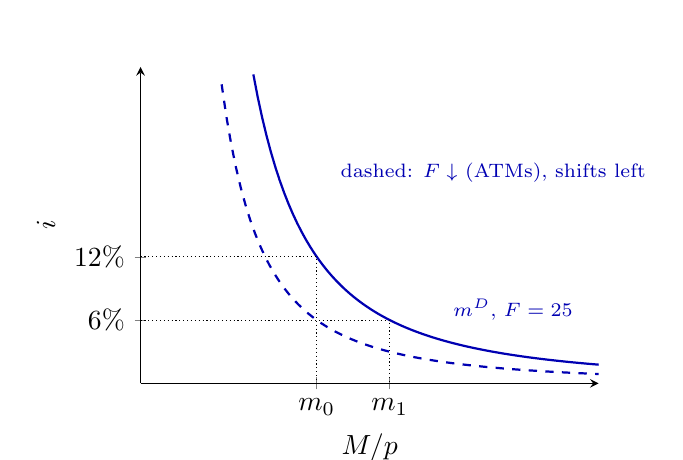
\begin{tikzpicture}
\begin{axis}[width=7.4cm,height=5.6cm,axis lines=left,xmin=0,xmax=6500,ymin=0,ymax=0.3,
  xlabel={$M/p$},ylabel={$i$},xtick={2500,3535.5},xticklabels={$m_0$,$m_1$},ytick={0.06,0.12},
  yticklabels={6\%,12\%},scaled x ticks=false,clip=false]
\addplot[thick,blue!70!black,domain=1600:6500,samples=80]{750000/x^2};
\addplot[thick,blue!70!black,dashed,domain=1150:6500,samples=80]{375000/x^2};
\addplot[densely dotted] coordinates {(0,0.12) (2500,0.12) (2500,0)};
\addplot[densely dotted] coordinates {(0,0.06) (3535.5,0.06) (3535.5,0)};
\node[font=\scriptsize,blue!70!black,anchor=west] at (axis cs:4300,0.07) {$m^D$, $F=25$};
\node[font=\scriptsize,blue!70!black,anchor=west] at (axis cs:2700,0.2) {dashed: $F\downarrow$ (ATMs), shifts left};
\end{axis}
\end{tikzpicture}
\end{center}
{\footnotesize Downward-sloping in $i$ (elasticity $-\tfrac12$); a lower $F$ shifts the whole curve left
(fewer balances at every $i$). Points used in (b): $i=12\%$ and $6\%$.}
\intuicao{Holding cash costs interest; refilling it costs trips. Doubling spending does not double cash, because the
trip cost is fixed: the optimal number of trips rises too.}
\refbib{Kurlat ch.~10, \S10.4, pp.~199--204, eqs.~(10.4.3)--(10.4.4); the exercise on ATMs, ex.~10.4, p.~203,
is related practice.}
\rubrica{
\item Average cash $pY/2N$ and the cost function: 0.15. $N^*$ and $M/p$ derived: 0.15.
\item Both elasticities and $V=2N$: 0.1. Numbers 12, 2{,}500, 24: 0.1 (slip: $-0.1$).
\item Graph with $i$ and $M/p$ on the axes and the shift for $F\downarrow$: 0.1.
\item Quoting $\sqrt{FY/2i}$ without deriving it: max.\ 0.2 on the item.
}
\end{sol}

\parte{b}{0.7 point} Using money-market equilibrium $M=p\,m^D(Y,i)$, derive the steady-state inflation rate when
$Y$ grows at $g$ and $i$ is constant, and compute $\pi$ and $i$. In mid-1994 the central bank cuts money growth
permanently and credibly to $\mu=5\%$. Find the new $\pi$ and $i$ and the change in real balances. Since the stock
of money does not jump by itself, what must happen to the price level on the day of the reform? Which one-time
change in $M$ would avoid it? Draw $\ln M$ and $\ln p$ around the reform, with that one-time change. A commentator
writes: ``After the Real, M1 rose by tens of percent while inflation collapsed, so money does not cause inflation.''
Evaluate.
\resolespaco
\begin{sol}
\begin{notacao}
\item Symbols of (a) keep their meaning. New here:
\item $m^D(Y,i)$: real money demand, \eqref{q3a:md}. A dot is a time derivative ($\dot M=dM/dt$).
\item $\mu\equiv\dot M/M$: money growth. $\pi\equiv\dot p/p$: inflation. $g\equiv\dot Y/Y$: real growth.
$r$: real interest rate. All per year.
\item $T$: date of the reform. $m_0$, $m_1$: real balances before and after; $p_{\text{old}}$, $p_{\text{new}}$:
price level just before and just after.
\end{notacao}
\passo{1 --- differentiate}{Money-market equilibrium at every date:
\begin{equation}
M_t=p_t\,m^D(Y_t,i_t). \label{q3b:mm}
\end{equation}
Differentiate \eqref{q3b:mm} with respect to $t$:
\begin{equation}
\dot M=\dot p\,m^D+p\Big(\frac{\partial m^D}{\partial Y}\dot Y+\frac{\partial m^D}{\partial i}\dot i\Big).
\label{q3b:diff}
\end{equation}
Set $\dot i=0$ and divide \eqref{q3b:diff} by \eqref{q3b:mm}:
\begin{align}
\frac{\dot M}{M} &= \frac{\dot p\,m^D+p\big(\frac{\partial m^D}{\partial Y}\dot Y+\frac{\partial m^D}{\partial i}(0)\big)}{p\,m^D}
\nonumber\\
&= \frac{\dot p}{p}+\underbrace{\frac{\partial m^D}{\partial Y}\frac{Y}{m^D}}_{\eta}
\frac{\dot Y}{Y}\nonumber\\
\mu &= \pi+\eta g\nonumber\\
\pi &= \mu-\eta g, \label{q3b:pi}
\end{align}
with $\eta=\tfrac12$ from \eqref{q3a:ln}. Kurlat's Fisher equation, from the statement:
\begin{equation}
i=r+\pi. \label{q3b:fisher}
\end{equation}}
\passo{2 --- before}{By \eqref{q3b:pi} and then \eqref{q3b:fisher}:
\begin{align*}
\pi &= 11\%-\tfrac12(4\%)=\boxed{9\%},\\
i &= 3\%+9\%=\boxed{12\%}
\end{align*}
(exact Fisher: $1.03\cdot1.09-1=12.27\%$).}
\passo{3 --- after}{With $\mu=5\%$, by \eqref{q3b:pi} and \eqref{q3b:fisher}:
\begin{align*}
\pi &= 5\%-\tfrac12(4\%)=\boxed{3\%},\\
i &= 3\%+3\%=\boxed{6\%}
\end{align*}
(Fisher effect: $i$ falls one-for-one with $\pi$, $r$ unchanged). Real balances, from the ratio of
\eqref{q3a:md} at the two rates:
\begin{align*}
\frac{m_1}{m_0} &= \frac{\sqrt{FY/(2i_1)}}{\sqrt{FY/(2i_0)}}\\
&= \sqrt{\frac{i_0}{i_1}}\\
&= \sqrt{\frac{0.12}{0.06}}\\
&= \sqrt2=1.414,
\end{align*}
$\boxed{+41.4\%}$ ($2{,}500\to3{,}536$). The jump is immediate: a credible reform changes expected inflation,
hence $i$, at once.}
\passo{4 --- the price level}{Solve \eqref{q3b:mm} for the price level:
\begin{equation}
p=\frac{M}{m^D}. \label{q3b:p}
\end{equation}
If $M$ is continuous and $m^D$ jumps by $\sqrt2$, \eqref{q3b:p} makes $p$ jump \emph{down}:
\begin{align*}
\frac{p_{\text{new}}}{p_{\text{old}}} &= \frac{M/m_1}{M/m_0}\\
&= \frac{m_0}{m_1}\\
&= \frac{1}{\sqrt2}=0.707,
\end{align*}
a $\boxed{29.3\%}$ fall in the price level. To keep $p$ continuous in \eqref{q3b:p}, $M$ must jump with $m^D$:
the central bank issues a one-time injection
\[
\boxed{\frac{\Delta M}{M}=\sqrt2-1=41.4\%}
\]
on the day of the reform (remonetisation), and \emph{from then on} money grows at 5\%. This injection is not
inflationary: it only meets the higher demand for real balances.}
\begin{center}
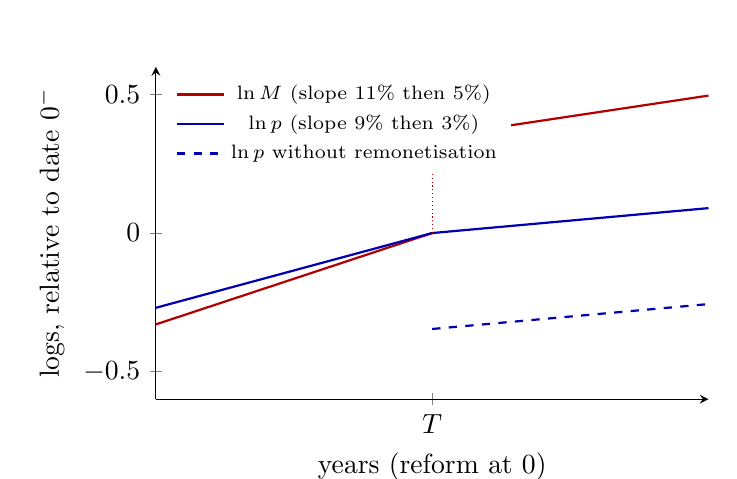
\begin{tikzpicture}
\begin{axis}[width=8.6cm,height=5.8cm,axis lines=left,xmin=-3,xmax=3,ymin=-0.6,ymax=0.6,
  xlabel={years (reform at $0$)},ylabel={logs, relative to date $0^-$},xtick={0},xticklabels={$T$},
  legend style={font=\scriptsize,draw=none,at={(0.02,0.98)},anchor=north west}]
\addplot[thick,red!70!black] coordinates {(-3,-0.33) (0,0)};
\addplot[thick,blue!70!black] coordinates {(-3,-0.27) (0,0)};
\addplot[thick,blue!70!black,dashed] coordinates {(0,-0.3466) (3,-0.2566)};
\addplot[thick,red!70!black,forget plot] coordinates {(0,0.3466) (3,0.4966)};
\addplot[thick,blue!70!black,forget plot] coordinates {(0,0) (3,0.09)};
\addplot[densely dotted,red!70!black,forget plot] coordinates {(0,0) (0,0.3466)};
\legend{$\ln M$ (slope 11\% then 5\%),$\ln p$ (slope 9\% then 3\%),$\ln p$ without remonetisation}
\end{axis}
\end{tikzpicture}\\
{\footnotesize With remonetisation $\ln M$ jumps by $\ln\sqrt2=0.35$ and $\ln p$ only changes slope. Without it,
$\ln M$ is continuous and $\ln p$ jumps down by $0.35$.}
\end{center}
\passo{5 --- the commentator}{Wrong inference. \eqref{q3b:pi} holds \emph{with $i$ constant}; at the reform $i$
falls and real money demand rises by about 41\%, so a one-time rise in $M$ of that size is exactly what keeps
prices stable. It is a \emph{level} adjustment of $M$ to a higher $m^D$, not sustained money growth. The theory
predicts both facts at once: the money stock jumps and inflation falls, because $\mu$ after the jump is low.}
\intuicao{When people expect inflation to fall, holding cash becomes cheaper and they want more of it. Either the
central bank supplies that cash, or prices fall until existing cash is worth enough.}
\refbib{Kurlat ch.~11, \S11.2, pp.~209--212, eq.~(11.2.3); \S11.1--\S11.2 on neutrality, pp.~205--215.}
\rubrica{
\item Total differentiation with $\dot i=0$ stated and $\eta$ named: 0.15. $\pi=9\%$, $i=12\%$: 0.05.
\item $\pi=3\%$, $i=6\%$, $m$ up by $\sqrt2$: 0.15. Using $\eta=1$ (quantity theory) instead of $\tfrac12$: $-0.1$.
\item Price-level jump of $-29.3\%$ or remonetisation of $41.4\%$: 0.15. Graph (slopes and the jump): 0.1.
\item Commentator: level vs growth, $m^D$ rising with lower $i$: 0.1. Agreeing with the commentator: 0 on this line.
}
\end{sol}

\parte{c}{0.6 point} Seigniorage. Compute real seigniorage per household before and after the reform, and split it
into the inflation tax and the part due to growth. Show that with the money demand of (a) seigniorage rises with
$\mu$ for every $\mu$, so there is no revenue-maximising money growth. Contrast with a Cagan semi-log demand
$M/p=Y e^{-a i}$, $a>0$: find the revenue-maximising $\mu$ and evaluate it for $a=2$. Draw both curves. Which demand
is consistent with Brazil's 1989--1993 experience, when money grew by more than 1{,}000\% a year?
\resolespaco
\begin{sol}
\begin{notacao}
\item Symbols of (a)--(b) keep their meaning. New here:
\item $S$: real seigniorage per household per year, the real value of newly issued money.
\item $a>0$: semi-elasticity of the Cagan demand $M/p=Ye^{-ai}$ with respect to $i$ ($a=2$).
\item $\mu^{\max}$: the money growth that maximises $S$ (the peak of the seigniorage Laffer curve).
\end{notacao}
\passo{1 --- definition}{Real seigniorage, multiplying and dividing by $M$:
\begin{align}
S\equiv\frac{\dot M}{p} &= \frac{\dot M}{M}\cdot\frac{M}{p}\nonumber\\
&= \mu\,m. \label{q3c:S}
\end{align}
Substitute $\mu=\pi+\eta g$ from \eqref{q3b:pi} into \eqref{q3c:S}:
\begin{align}
S &= (\pi+\eta g)\,m\nonumber\\
&= \underbrace{\pi m}_{\text{inflation tax}}+\underbrace{\eta g\,m}_{\text{growth}}. \label{q3c:split}
\end{align}}
\passo{2 --- numbers}{Before ($\mu=11\%$, $\pi=9\%$, $m=2{,}500$), by \eqref{q3c:S} and \eqref{q3c:split}:
\begin{align*}
S &= 0.11\cdot2{,}500=\boxed{275},\\
\pi m+\eta g\,m &= 0.09\cdot2{,}500+\tfrac12(0.04)\cdot2{,}500=225+50,
\end{align*}
$0.46\%$ of $Y$. After ($\mu=5\%$, $\pi=3\%$, $m=3{,}536$):
\begin{align*}
S &= 0.05\cdot3{,}536=\boxed{176.8},\\
\pi m+\eta g\,m &= 0.03\cdot3{,}536+\tfrac12(0.04)\cdot3{,}536=106.1+70.7,
\end{align*}
$0.29\%$ of $Y$. Revenue falls by 36\%, much less than $\mu$ (by 55\%), because the base rises 41\%; and the
growth part \emph{rises}: a growing economy absorbs new money without inflation.}
\passo{3 --- no peak under Baumol--Tobin}{Substitute \eqref{q3b:pi} into \eqref{q3b:fisher}:
\begin{align}
i &= r+(\mu-\eta g)\nonumber\\
&= 0.03+\mu-\tfrac12(0.04)\nonumber\\
&= \mu+0.01. \label{q3c:i}
\end{align}
Substitute \eqref{q3a:md} with \eqref{q3c:i} into \eqref{q3c:S}:
\begin{align}
S &= \mu\left(\sqrt{\frac{FY}{2i}}\right)\nonumber\\
S(\mu) &= \mu\sqrt{\frac{FY}{2(\mu+r-\eta g)}}. \label{q3c:Sbt}
\end{align}
Differentiate the log of \eqref{q3c:Sbt}, using $di/d\mu=1$ and $2i-\mu=\mu+2(r-\eta g)$:
\begin{align*}
\frac{d\ln S}{d\mu} &= \frac1\mu-\frac{1}{2i}\\
&= \frac{2i-\mu}{2\mu i}\\
&= \frac{2(\mu+r-\eta g)-\mu}{2\mu i}\\
&= \frac{\mu+2(r-\eta g)}{2\mu i}>0
\end{align*}
for all $\mu>0$, since $r-\eta g=1\%>0$. Equivalently, the elasticity of the base with respect to $\mu$ is $-\mu/(2i)>-\tfrac12>-1$: the base never shrinks
fast enough to offset the rate. \#~The Laffer peak needs a base elasticity of $-1$.}
\passo{4 --- Cagan}{The Cagan demand:
\begin{equation}
\frac Mp=Ye^{-ai}. \label{q3c:cagan}
\end{equation}
Substitute \eqref{q3c:cagan} with \eqref{q3c:i} into \eqref{q3c:S}:
\begin{align}
S &= \mu\big(Ye^{-ai}\big)\nonumber\\
&= \mu Y e^{-a(r-\eta g+\mu)}. \label{q3c:Scagan}
\end{align}
Differentiate \eqref{q3c:Scagan} with respect to $\mu$ and set it to zero:
\begin{align*}
\frac{dS}{d\mu} &= Ye^{-a(\cdot)}\,(1-a\mu)=0\\
\Rightarrow\ \mu^{\max} &= 1/a.
\end{align*}
SOC: $\frac{d^2S}{d\mu^2}=-aYe^{-a(\cdot)}(2-a\mu)<0$ at $\mu=1/a$. With $a=2$:
$\boxed{\mu^{\max}=1/a=1/2=50\%}$ a year.}
\begin{center}
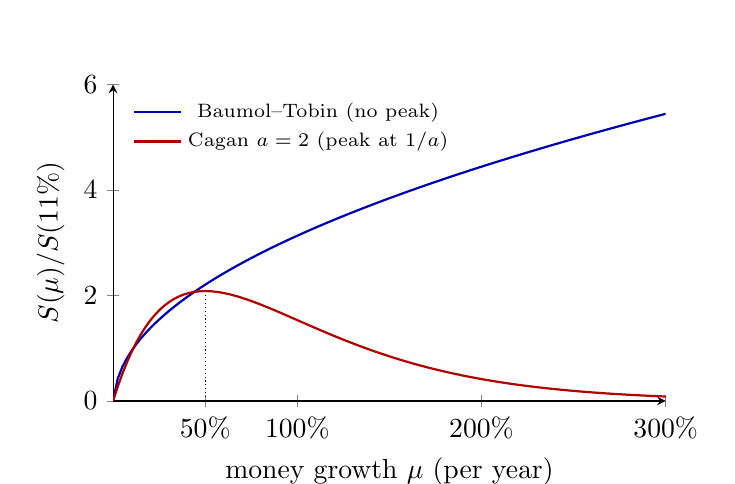
\begin{tikzpicture}
\begin{axis}[width=8.6cm,height=5.6cm,axis lines=left,xmin=0,xmax=3,ymin=0,ymax=6,
  xlabel={money growth $\mu$ (per year)},ylabel={$S(\mu)/S(11\%)$},xtick={0.5,1,2,3},
  xticklabels={50\%,100\%,200\%,300\%},
  legend style={font=\scriptsize,draw=none,at={(0.02,0.98)},anchor=north west}]
\addplot[thick,blue!70!black,domain=0:3,samples=120]{x/sqrt(x+0.01)/0.31754};
\addplot[thick,red!70!black,domain=0:3,samples=120]{x*exp(-2*(x+0.01))/0.086530};
\addplot[densely dotted] coordinates {(0.5,0) (0.5,2.0837)};
\legend{Baumol--Tobin (no peak),Cagan $a=2$ (peak at $1/a$)}
\end{axis}
\end{tikzpicture}
\end{center}
\passo{5 --- Brazil}{Rising revenue at any $\mu$, as \eqref{q3c:Sbt} implies, cannot explain why governments
printing over 1{,}000\% a year did not raise ever more revenue; with a Cagan demand \eqref{q3c:Scagan} they were
far on the \emph{wrong side} of the Laffer curve, where cutting $\mu$ costs little revenue or even raises it.
Baumol--Tobin with a fixed $F$ misses the flight from money at high inflation (indexed overnight accounts lowered
the effective $F$ and made demand far more elastic).}
\intuicao{Seigniorage is a tax with rate $\mu$ on the base $M/p$. Whether raising the rate raises revenue depends on
how fast the base flees; under Baumol--Tobin it flees too slowly to ever turn revenue down.}
\refbib{Kurlat ch.~11, \S11.3, pp.~215--216 (seigniorage); the Cagan demand is used in ex.~11.6, p.~218, which
works the limit on revenue with another functional form.}
\rubrica{
\item $S=\mu m$ and the split: 0.1. Both numbers and splits: 0.15 (slip: $-0.1$).
\item Proof of no peak (derivative signed, or elasticity $>-1$): 0.15. Asserting it without proof: 0 on this line.
\item Cagan peak with SOC and 50\%: 0.1. Graph (both curves, peak marked): 0.05.
\item Brazil reading: 0.05.
}
\end{sol}

\parte{d}{0.6 point} Costs of inflation. Compute the real resources spent on trips to the bank, in reais and as a
share of $Y$, before and after the reform. Why is the forgone interest on cash not counted as a cost to society?
Find the inflation and money-growth rates of the Friedman rule, and say what happens to the Baumol--Tobin solution
there. Give two reasons why the central bank targets 3\% rather than this rate.
\resolespaco
\begin{sol}
\begin{notacao}
\item Symbols of (a)--(c) keep their meaning. New here:
\item $R\ge0$: real resources spent on trips to the bank per year (shoe-leather cost), $R=FN^*$.
\item Friedman rule: the policy that sets the nominal interest rate to zero, $i=0$.
\end{notacao}
\passo{1 --- trips}{The resource cost is the number of trips times their real cost. Substitute
\eqref{q3a:N}:
\begin{align}
R=FN^* &= F\left(\sqrt{\frac{iY}{2F}}\right)\nonumber\\
&= \boxed{\sqrt{\frac{iFY}{2}}}. \label{q3d:R}
\end{align}
Before ($i=12\%$, $N^*=12$) and after ($i=6\%$), by \eqref{q3d:R}:
\begin{align*}
R_{\text{before}} &= 25\cdot12=\boxed{300},\quad 0.50\%\ \text{of }Y,\\
R_{\text{after}} &= \sqrt{\frac{0.06\cdot25\cdot60{,}000}{2}}=\sqrt{45{,}000}=\boxed{212.1},\quad 0.35\%\ \text{of }Y.
\end{align*}
The reform saves $0.15\%$ of income every year (shoe-leather cost).}
\passo{2 --- forgone interest}{Multiply \eqref{q3a:md} by $i$: at the optimum the forgone interest is
\[
i\,\frac Mp=i\left(\sqrt{\frac{FY}{2i}}\right)=\sqrt{\frac{iFY}{2}},
\]
the same as \eqref{q3d:R} (300 before), but it is not a use of resources: the inflation-tax part
($\pi m=225$, \eqref{q3c:split}) is revenue of the government, and the rest is a transfer to whoever borrows the
funds. Only the trips burn goods. (Total private cost $\sqrt{2iFY}=600$.)}
\passo{3 --- Friedman rule}{Set $i=0$ in \eqref{q3b:fisher}, then use \eqref{q3b:pi} solved for $\mu$:
\begin{align*}
(0) &= r+\pi\\
\pi &= -r=\boxed{-3\%},\\
\mu &= \pi+\eta g=(-3\%)+\tfrac12(4\%)=\boxed{-1\%}.
\end{align*}
Then, by \eqref{q3a:N} and \eqref{q3a:md}, $N^*\to0$ and $M/p\to\infty$. The interior solution needs $N^*\ge1$;
by \eqref{q3a:N}:
\[
\frac{iY}{2F}\ge1\iff i\ge\frac{2F}{Y}=\frac{2\cdot25}{60{,}000}=0.083\%;
\]
below that the household makes one trip and holds $Y/2=30{,}000$. Shoe-leather costs vanish.}
\passo{4 --- why 3\%}{(i) Measured inflation overstates true inflation (substitution, quality and new-goods biases
of a Laspeyres index), so 0 measured is deflation. (ii) With $\pi=-3\%$, $i$ would sit at zero in normal times,
leaving no room to cut it in a recession --- the zero lower bound of Question 4. (iii) Nominal wages are rigid
downward; some inflation lets real wages fall.}
\intuicao{Inflation is a tax on holding cash; people spend real resources dodging it. The Friedman rule removes the
tax, but a central bank that needs room to cut rates gives up a little of that gain.}
\refbib{Kurlat ch.~11, \S11.4, pp.~216--222 (costs of inflation, Friedman rule); ch.~10, \S10.4.}
\rubrica{
\item Trip cost formula and both numbers with shares: 0.2 (slip: $-0.1$). Counting $i\,m$ as the social cost: max.\ 0.1 on this line.
\item Transfer argument: 0.1. Friedman rule $\pi=-3\%$, $\mu=-1\%$: 0.1; the corner $N\ge1$: 0.05.
\item Two valid reasons for a positive target: 0.15.
}
\gap{Kurlat ch.~10--11 were absent from Prova 01: Baumol--Tobin from primitives, $\pi=\mu-\eta g$ by total
differentiation, Fisher, seigniorage and its Laffer curve.}
\end{sol}

% =============================================================================
\questao{(3.0 points) The Copom between a tax shock and a liquidity trap.
Use Benigno (2015), in log deviations from an efficient steady state, with a short run and a long run:
\begin{align}
y &= \bar y_n+(g-\bar g)-\sigma\left[i-(\bar p-p)-\rho\right], \tag{AD}\label{q4:AD}\\
p-p^e &= \kappa(y-y_n), \tag{AS}\label{q4:AS}\\
y_n &= \frac{(1+\eta)a+\sigma^{-1}g-\mu}{\sigma^{-1}+\eta}, \tag{YN}\label{q4:YN}\\
y_e &= \frac{(1+\eta)a+\sigma^{-1}g}{\sigma^{-1}+\eta}. \tag{YE}\label{q4:YE}
\end{align}
Initially $a=g=\bar g=\mu=0$, $\bar y_n=0$, $\bar p=p^e=0$ and $i=\rho$. Take $\sigma=1$, $\eta=1$, $\kappa=1/2$ and
$\rho=2\%$; $y$ and $p$ are in percent. The Copom sets $i$ to minimise
\begin{equation}
L=\tfrac12(y-y_e)^2+\frac{\phi}{2\kappa}(p-p^e)^2,\qquad \phi>0. \tag{LF}\label{q4:LF}
\end{equation}}

\parte{a}{0.8 point} A temporary rise in a federal tax on firms' revenues raises the mark-up by $\mu=4$ in the
current period only. Find the changes in $y_n$ and $y_e$ and say which curve shifts. Derive the Copom's optimal
targeting rule by substituting the relevant constraint into the loss, and the optimal $y$ and $p$ as functions of
$\phi$; evaluate them for $\phi=4$. Explain why the Copom cannot reach $y=y_e$ and $p=p^e$ together here, while it
could after a temporary productivity shock. Show graphically.
\resolespaco
\begin{sol}
\begin{notacao}
\item $y$, $p$: output and price level today, log deviations from the steady state, in percent.
\item $\bar y_n$, $\bar p$: long-run natural output and long-run price level. $p^e$: the price preset by firms
that cannot adjust this period.
\item $i\ge0$: nominal policy rate, the Copom's instrument. $\rho>0$: rate of time preference, the steady-state
real rate ($\rho=2\%$).
\item $g$, $\bar g$: government spending today and in the long run. $a$: productivity. $\mu$: firms' mark-up
(here raised by the tax).
\item $\sigma>0$: intertemporal elasticity of substitution (not the capital share of Q1). $\eta>0$: inverse
Frisch elasticity of labour supply. $\kappa>0$: slope of AS.
\item $y_n$: natural output (flexible prices, with the mark-up). $y_e$: efficient output (no mark-up).
\item $\phi>0$: weight on price surprises in the loss $L$ \eqref{q4:LF}.
\item $\Delta\equiv y_e-y_n$: the gap between efficient and natural output (defined in Step 1).
\item $y^*$, $p^*$: the optimal point. $E_0$: initial equilibrium. $E'$: the outcome with $i=\rho$. $O$: the optimum.
\end{notacao}
\passo{1 --- what moves}{Differentiate \eqref{q4:YN} and \eqref{q4:YE} with respect to $\mu$:
\begin{align}
dy_n &= -\frac{\mu}{\sigma^{-1}+\eta}=-\frac{4}{1+1}=\boxed{-2}, \label{q4a:dyn}\\
dy_e &= \boxed{0}\qquad(\mu\text{ is not in }y_e). \label{q4a:dye}
\end{align}
\textbf{AS shifts up/left}: by \eqref{q4:AS} it now passes through $(y_n',p^e)=(-2,0)$, so at each $y$ the price
is higher by $\kappa\cdot2=1$. \textbf{AD does not move}: $\mu$ is not in \eqref{q4:AD} and, the shock being
temporary, $\bar y_n$ is unchanged. From \eqref{q4a:dyn}--\eqref{q4a:dye}:
\begin{equation}
\Delta\equiv y_e-y_n=0-(-2)=2>0. \label{q4a:Delta}
\end{equation}}
\passo{2 --- the constraint}{The Copom moves AD with $i$, so it can pick \emph{any} point on AS; AS ($p^e$ is
predetermined) is the constraint. Substitute \eqref{q4:AS} into \eqref{q4:LF}:
\begin{align}
L(y) &= \tfrac12(y-y_e)^2+\frac{\phi}{2\kappa}\big(\kappa(y-y_n)\big)^2\nonumber\\
&= \tfrac12(y-y_e)^2+\frac{\phi}{2\kappa}\kappa^2(y-y_n)^2\nonumber\\
&= \tfrac12(y-y_e)^2+\frac{\phi\kappa}{2}(y-y_n)^2. \label{q4a:Ly}
\end{align}}
\passo{3 --- targeting rule}{Differentiate \eqref{q4a:Ly} and set it to zero (SOC $1+\phi\kappa>0$):
\begin{equation}
\frac{dL}{dy}=(y-y_e)+\phi\kappa(y-y_n)=0. \label{q4a:foc}
\end{equation}
By \eqref{q4:AS}, $\kappa(y-y_n)=p-p^e$. Substitute this into \eqref{q4a:foc}:
\begin{equation}
\boxed{(y-y_e)+\phi\,(p-p^e)=0}. \label{q4a:rule}
\end{equation}
Solve \eqref{q4a:foc} for $y$, then use $y_e=0$ and $y_n=-\Delta$ from \eqref{q4a:Delta}:
\begin{align}
y(1+\phi\kappa) &= y_e+\phi\kappa\,y_n\nonumber\\
y^* &= \frac{y_e+\phi\kappa\,y_n}{1+\phi\kappa}\nonumber\\
&= \frac{(0)+\phi\kappa\,(-\Delta)}{1+\phi\kappa}\nonumber\\
&= -\frac{\phi\kappa\,\Delta}{1+\phi\kappa}. \label{q4a:ystar}
\end{align}
Subtract $y_n=-\Delta$ from \eqref{q4a:ystar} and substitute into \eqref{q4:AS}:
\begin{align}
y^*-y_n &= \left(-\frac{\phi\kappa\,\Delta}{1+\phi\kappa}\right)-(-\Delta)\nonumber\\
&= \frac{\Delta}{1+\phi\kappa},\nonumber\\
p^*-p^e &= \kappa(y^*-y_n)\nonumber\\
&= \kappa\left(\frac{\Delta}{1+\phi\kappa}\right)\nonumber\\
&= \frac{\kappa\,\Delta}{1+\phi\kappa}. \label{q4a:pstar}
\end{align}
With $\phi=4$, $\phi\kappa=2$; by \eqref{q4a:ystar} and \eqref{q4a:pstar}:
\begin{align*}
y^* &= -\frac{2\cdot2}{1+2}=\boxed{-1.33\%},\\
p^* &= \frac{0.5\cdot2}{1+2}=\boxed{+0.33\%}.
\end{align*}
Check in \eqref{q4a:rule}: $-\tfrac43+4\cdot\tfrac13=0$ \checkmark.}
\passo{4 --- divine coincidence fails}{Both targets require $y=y_e=0$ and $p=p^e$, but on the new AS
\eqref{q4:AS}, $p-p^e=\kappa(0+2)=1\neq0$ at $y=0$: the bliss point is not on the constraint, and one instrument
cannot hit two targets. After a temporary productivity shock, \eqref{q4:YN} and \eqref{q4:YE} move $y_n$ and $y_e$
by the same $\frac{1+\eta}{\sigma^{-1}+\eta}a$, so $(y_e,p^e)$ lies on the new AS and the Copom puts AD through it:
zero loss, whatever $\phi$.}
\begin{center}
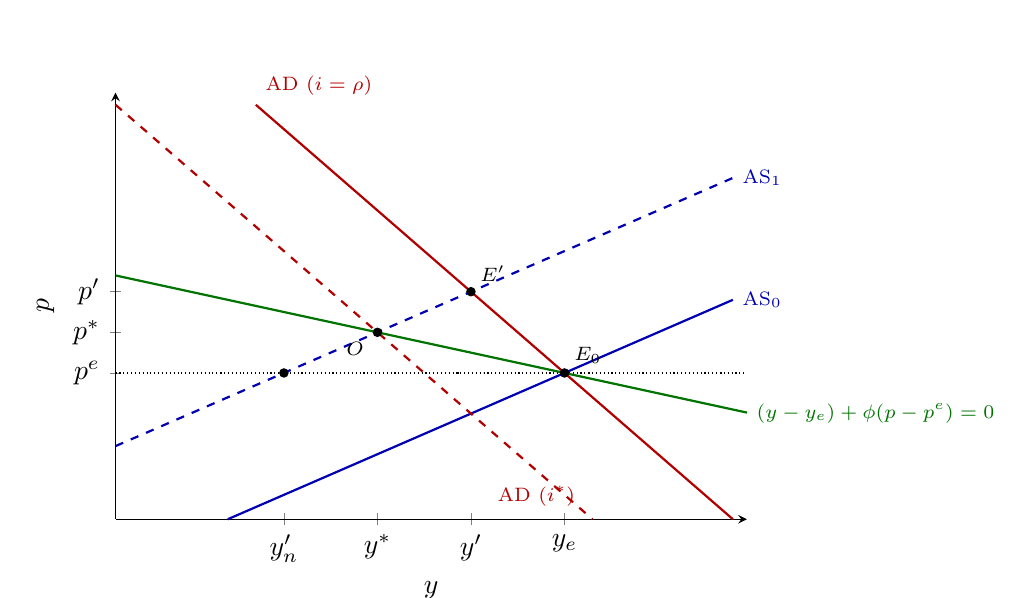
\begin{tikzpicture}
\begin{axis}[width=9.6cm,height=7cm,axis lines=left,xmin=-3.2,xmax=1.3,ymin=-1.2,ymax=2.3,clip=false,
  xlabel={$y$},ylabel={$p$},
  xtick={-2,-1.3333,-0.6667,0},xticklabels={$y_n'$,$y^*$,$y'$,$y_e$},ytick={0,0.3333,0.6667},
  yticklabels={$p^e$,$p^*$,$p'$}]
\addplot[densely dotted,domain=-3.2:1.3]{0};
\addplot[thick,blue!70!black,domain=-2.4:1.2]{0.5*x};
\addplot[thick,blue!70!black,dashed,domain=-3.2:1.2]{0.5*(x+2)};
\addplot[thick,red!70!black,domain=-2.2:1.2]{-x};
\addplot[thick,red!70!black,dashed,domain=-3.2:0.2]{-x-1};
\addplot[thick,green!45!black,domain=-3.2:1.3]{-x/4};
\addplot[only marks,mark=*,mark size=1.5pt] coordinates {(0,0) (-0.6667,0.6667) (-1.3333,0.3333) (-2,0)};
\node[font=\scriptsize,blue!70!black,anchor=west] at (axis cs:1.2,0.6) {AS$_0$};
\node[font=\scriptsize,blue!70!black,anchor=west] at (axis cs:1.2,1.6) {AS$_1$};
\node[font=\scriptsize,red!70!black,anchor=south west] at (axis cs:-2.2,2.2) {AD ($i=\rho$)};
\node[font=\scriptsize,red!70!black,anchor=north] at (axis cs:-0.2,-0.85) {AD ($i^*$)};
\node[font=\scriptsize,green!45!black,anchor=west] at (axis cs:1.3,-0.33) {$(y-y_e)+\phi(p-p^e)=0$};
\node[font=\scriptsize,anchor=south west] at (axis cs:-0.67,0.67) {$E'$};
\node[font=\scriptsize,anchor=north east] at (axis cs:-1.36,0.33) {$O$};
\node[font=\scriptsize,anchor=south west] at (axis cs:0,0) {$E_0$};
\end{axis}
\end{tikzpicture}\\
{\footnotesize AS shifts up through $(y_n',p^e)$; with $i=\rho$ the economy goes to $E'=(-0.67,\,0.67)$ along the
unmoved AD. The optimum $O=(-1.33,\,0.33)$ is where AS$_1$ meets the targeting line (slope $-1/\phi$, through
the bliss point $E_0$); the Copom raises $i$ to move AD down to $O$.}
\end{center}
\intuicao{A mark-up shock makes the economy's natural output inefficiently low. Pushing output up to the efficient
level costs inflation; holding prices costs output. With convex losses the Copom splits the difference, and $\phi$
says how much it dislikes the price side.}
\refbib{Benigno (2015), \S7 (mark-up shocks), Fig.~9, pp.~513--514; \S11, eqs.~(33)--(35), Fig.~14, pp.~521--523;
\S4.2--\S4.4 for $y_n$ vs $y_e$, pp.~508--509.}
\rubrica{
\item $dy_n=-2$, $dy_e=0$, AS shifts and AD does not, with reasons: 0.2. Shifting AD: max.\ 0.3 on the item.
\item Substituting AS into the loss and $dL/dy=0$; the targeting rule: 0.2. Minimising along AD or treating $i$ as
the choice with AD as the constraint: max.\ 0.3 on the item.
\item $y^*$, $p^*$ in general and $-1.33$, $+0.33$: 0.15 (slip: $-0.1$).
\item Divine-coincidence argument and the productivity contrast: 0.1.
\item Graph: axes, AS$_0$/AS$_1$, AD, the targeting line, $E'$ and $O$: 0.15.
}
\end{sol}

\parte{b}{0.6 point} Find the policy rate $i^*$ that implements the optimum, for general $\phi$ and for $\phi=4$, and
compare it with keeping $i=\rho$. Show that the Copom raises the rate if and only if $\phi>\sigma$. Interpret
$\phi\to0$, $\phi\to\infty$ and the knife edge $\phi=\sigma$, using the graph of (a).
\resolespaco
\begin{sol}
\begin{notacao}
\item Symbols of (a) keep their meaning. New here:
\item $i^*$: the policy rate that implements $(y^*,p^*)$.
\item $y'$, $p'$: the outcome if the Copom keeps $i=\rho$ (point $E'$).
\end{notacao}
\passo{1 --- invert AD}{Set $\bar y_n=g=\bar g=\bar p=0$ in \eqref{q4:AD}:
\begin{align}
y &= (0)+(0-0)-\sigma\big[i-(0-p)-\rho\big]\nonumber\\
&= -\sigma(i-\rho)-\sigma p. \label{q4b:ad}
\end{align}
Solve \eqref{q4b:ad} for the rate:
\begin{equation}
i-\rho=-\frac{y+\sigma p}{\sigma}. \label{q4b:inv}
\end{equation}}
\passo{2 --- the rate}{Add \eqref{q4a:ystar} and $\sigma$ times \eqref{q4a:pstar} (with $p^e=0$):
\begin{align*}
y^*+\sigma p^* &= \left(-\frac{\phi\kappa\Delta}{1+\phi\kappa}\right)+\sigma\left(\frac{\kappa\Delta}{1+\phi\kappa}\right)\\
&= \frac{-\phi\kappa\Delta+\sigma\kappa\Delta}{1+\phi\kappa}\\
&= -\frac{\kappa(\phi-\sigma)\Delta}{1+\phi\kappa}.
\end{align*}
Substitute into \eqref{q4b:inv}:
\begin{align}
i^*-\rho &= -\frac{1}{\sigma}\left(-\frac{\kappa(\phi-\sigma)\Delta}{1+\phi\kappa}\right)\nonumber\\
&= \boxed{\frac{\kappa(\phi-\sigma)\,\Delta}{\sigma(1+\phi\kappa)}}. \label{q4b:istar}
\end{align}
With $\phi=4$:
\[
i^*-\rho=\frac{0.5\cdot(4-1)\cdot2}{1\cdot(1+2)}=1\ \Rightarrow\ \boxed{i^*=3\%}.
\]
Check on \eqref{q4b:ad}: $-1\cdot(3-2)-1\cdot\tfrac13=-\tfrac43=y^*$ \checkmark. With $i=\rho$, \eqref{q4b:ad} gives
$y=-\sigma p$; substitute \eqref{q4:AS}, $p=\kappa(y-y_n')$:
\begin{align*}
y &= -\sigma\big(\kappa(y-y_n')\big)\\
y(1+\sigma\kappa) &= \sigma\kappa\,y_n'\\
y' &= \frac{\sigma\kappa}{1+\sigma\kappa}y_n'=\frac{0.5}{1.5}(-2)=-0.67,\\
p' &= -y'/\sigma=-(-0.67)/1=+0.67.
\end{align*}
Loss \eqref{q4:LF} ($\phi/2\kappa=4$) at $E'$ and at the optimum $O$:
\begin{align*}
L(E') &= \tfrac12\big(\tfrac23\big)^2+4\big(\tfrac23\big)^2=\tfrac29+\tfrac{16}9=2.0,\\
L(O) &= \tfrac12\big(\tfrac43\big)^2+4\big(\tfrac13\big)^2=\tfrac89+\tfrac49=1.33.
\end{align*}}
\passo{3 --- sign}{In \eqref{q4b:istar}, $\kappa,\Delta,\sigma,1+\phi\kappa>0$, so
\[
\operatorname{sign}(i^*-\rho)=\operatorname{sign}(\phi-\sigma):\quad\boxed{\text{raise iff }\phi>\sigma}.
\]
Doing nothing leaves, from the lines above, $y'-y_n'=\frac{\Delta}{1+\sigma\kappa}$; the optimum
\eqref{q4a:pstar} wants $y^*-y_n=\frac{\Delta}{1+\phi\kappa}$, smaller iff $\phi>\sigma$, which needs a lower AD,
i.e.\ a higher rate.}
\passo{4 --- limits}{Take limits in \eqref{q4b:istar}, \eqref{q4a:ystar} and \eqref{q4a:pstar}:
\begin{itemize}[leftmargin=1.4em]
\item $\phi\to0$: $i^*-\rho\to-\kappa\Delta=-1$, $i^*=1\%$: the Copom \emph{cuts}, sets $y=y_e=0$ and accepts
$p=+1\%$.
\item $\phi\to\infty$: $i^*-\rho\to\Delta/\sigma=2$, $i^*=4\%$: strict price stability, $p=p^e$, $y=y_n'=-2$.
\item $\phi=\sigma$: $i^*=\rho$.
\end{itemize}
Geometrically the targeting line \eqref{q4a:rule} (slope $-1/\phi$) and AD \eqref{q4b:ad} (slope $-1/\sigma$)
both pass through the bliss point $E_0$; when $\phi=\sigma$ they coincide, so AD at $i=\rho$ already meets AS$_1$
on the targeting line.}
\intuicao{Doing nothing already splits the shock between prices and output in a proportion set by $\sigma$ (how
strongly demand reacts to the real rate). The Copom tightens only if it cares about prices more than that
built-in split does.}
\refbib{Benigno (2015), \S11, pp.~521--523; \S5, eqs.~(20)--(21), pp.~509--511.}
\rubrica{
\item AD inverted and $i^*$ in general: 0.2; $i^*=3\%$ with the comparison to $i=\rho$: 0.1.
\item Sign proof ($\phi>\sigma$): 0.15. Stating the sign without proof: 0 on this line. Saying the response does not
depend on $\phi$ (true only for AD shocks): max.\ 0.2 on the item.
\item The three cases, each with its reading: 0.15.
}
\end{sol}

\parte{c}{0.7 point} Two years later the tax is gone ($\mu=0$), but a household-debt crisis makes households expect
lower long-run income: $\bar y_n$ falls by 4\%, with $y_n$ and $y_e$ unchanged. Find the natural real rate $r_n$ and
the rate the Copom would like to set. Given $i\ge0$, find $y$, $p$ and the gaps when $i=0$, and show the outcome
graphically. What promise about $\bar p$ would take the economy to $(y_e,p^e)$ with $i=0$, and what does it require?
\resolespaco
\begin{sol}
\begin{notacao}
\item Symbols of (a)--(b) keep their meaning; now $\mu=0$, so $y_n=y_e=0$. New here:
\item $\bar y_n=-4$: long-run natural output after the household-debt crisis.
\item $r_n$: the natural real rate, the $i$ that delivers $y=y_n$ with $p=p^e=\bar p$.
\item $i\ge0$: the zero lower bound (ZLB). $Z$: the outcome at $i=0$.
\end{notacao}
\passo{1 --- natural rate}{Put $y=y_n$, $p=p^e=\bar p$ (so $\bar p-p=0$), $g=\bar g=0$ and $i=r_n$ in
\eqref{q4:AD}:
\begin{align*}
y_n &= \bar y_n+(0-0)-\sigma\big[r_n-(0)-\rho\big]\\
&= \bar y_n-\sigma(r_n-\rho).
\end{align*}
Solve for $r_n$:
\begin{equation}
\boxed{r_n=\rho+\sigma^{-1}(\bar y_n-y_n)}. \label{q4c:rn}
\end{equation}
Numbers in \eqref{q4c:rn}: $r_n=2+1^{-1}(-4-0)=\boxed{-2\%}$. This is a pure AD shock (AS does not move), so the divine
coincidence holds and the Copom wants $i=r_n=-2\%$.}
\passo{2 --- the ZLB binds}{$i=-2\%$ is infeasible; the best it can do is $i=0$. Put $i=0$, $\bar y_n=-4$,
$\bar p=0$ in \eqref{q4:AD}:
\begin{align}
y &= (-4)+(0-0)-1\cdot\big[(0)-(0-p)-2\big]\nonumber\\
&= -2-p. \label{q4c:ad}
\end{align}
AS \eqref{q4:AS} with $p^e=0$, $y_n=0$, $\kappa=\tfrac12$:
\begin{align}
p-(0) &= \tfrac12\big(y-(0)\big)\nonumber\\
p &= \tfrac12y. \label{q4c:as}
\end{align}
Substitute \eqref{q4c:as} into \eqref{q4c:ad}:
\begin{align*}
y &= -2-\left(\tfrac12y\right)\\
\tfrac32y &= -2\\
y &= \boxed{-1.33\%}.
\end{align*}
Back into \eqref{q4c:as}: $p=\tfrac12(-\tfrac43)=\boxed{-0.67\%}$. Gaps: $y-y_n=y-y_e=\boxed{-1.33}$; prices fall.
Loss \eqref{q4:LF} with $\phi=4$:
\begin{align*}
L &= \tfrac12\left(-\tfrac43\right)^2+4\left(-\tfrac23\right)^2\\
&= \tfrac12(1.78)+4(0.44)=2.67.
\end{align*}}
\passo{3 --- forward guidance}{Keep $i=0$ but let $\bar p$ be free in \eqref{q4:AD}:
\begin{equation}
y=-4-\big[0-\bar p+p-2\big]. \label{q4c:fg}
\end{equation}
Require $(y,p)=(0,0)$ in \eqref{q4c:fg}:
\begin{align*}
(0) &= -4-\big[0-\bar p+(0)-2\big]\\
0 &= -4+\bar p+2\\
\bar p &= \boxed{+2\%=-r_n}.
\end{align*}
A higher future price level is expected inflation $\bar p-p=2$, which takes the real rate $i-(\bar p-p)$ to
$-2\%=r_n$ with $i=0$. It requires \textbf{credibility}: the Copom must convince people it will tolerate a higher
price level later, when it would be tempted to renege.}
\begin{center}
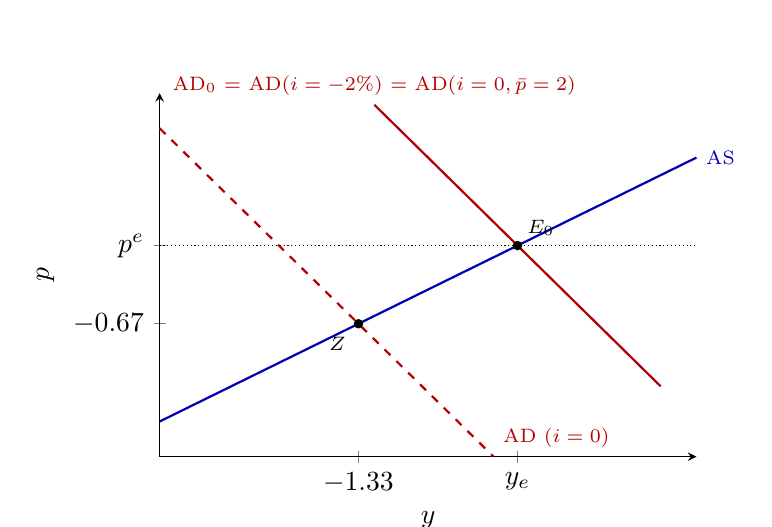
\begin{tikzpicture}
\begin{axis}[width=8.4cm,height=6.2cm,axis lines=left,xmin=-3,xmax=1.5,ymin=-1.8,ymax=1.3,clip=false,
  xlabel={$y$},ylabel={$p$},
  xtick={-1.3333,0},xticklabels={$-1.33$,$y_e$},ytick={-0.6667,0},yticklabels={$-0.67$,$p^e$}]
\addplot[densely dotted,domain=-3:1.5]{0};
\addplot[thick,blue!70!black,domain=-3:1.5]{0.5*x};
\addplot[thick,red!70!black,domain=-1.2:1.2]{-x};
\addplot[thick,red!70!black,dashed,domain=-3:-0.2]{-2-x};
\addplot[only marks,mark=*,mark size=1.5pt] coordinates {(0,0) (-1.3333,-0.6667)};
\node[font=\scriptsize,blue!70!black,anchor=west] at (axis cs:1.5,0.75) {AS};
\node[font=\scriptsize,red!70!black,anchor=south] at (axis cs:-1.2,1.2) {AD$_0$ $=$ AD($i=-2\%$) $=$ AD($i=0,\bar p=2$)};
\node[font=\scriptsize,red!70!black,anchor=south west] at (axis cs:-0.2,-1.8) {AD ($i=0$)};
\node[font=\scriptsize,anchor=north east] at (axis cs:-1.36,-0.70) {$Z$};
\node[font=\scriptsize,anchor=south west] at (axis cs:0,0) {$E_0$};
\end{axis}
\end{tikzpicture}\\
{\footnotesize The fall in $\bar y_n$ shifts AD left by 4; at $i=0$ it can only be brought back by 2, so the economy
sits at $Z$. Either $i=-2\%$ (infeasible) or $\bar p=2\%$ (a promise) puts AD back through $E_0$.}
\end{center}
\intuicao{Expecting to be poorer later, households cut consumption now. Only a negative real rate would persuade
them to spend; with $i$ stuck at zero, that negative real rate has to come from expected inflation.}
\refbib{Benigno (2015), \S9 (liquidity trap), Figs.~11--12, pp.~516--518; natural rate from \S5.}
\rubrica{
\item $r_n=-2\%$ derived and the desired $i$: 0.15. Calling it a supply shock or a trade-off: max.\ 0.2 on the item.
\item ZLB equilibrium $y=-1.33$, $p=-0.67$, gaps: 0.2 (slip: $-0.1$).
\item $\bar p=2\%$ and the real-rate mechanism, credibility: 0.2.
\item Graph: AS, AD shifted left, the partial return at $i=0$, point $Z$: 0.15.
}
\end{sol}

\parte{d}{0.9 point} Instead of a promise, the government raises current spending $g$ ($\bar g$ unchanged) while
$i$ stays at 0. Derive the multipliers $dy/dg$ and $d(y-y_e)/dg$, evaluate them, find the $g$ that closes the gap,
and check what happens to $p$. Then suppose the Copom were away from the ZLB and followed its optimal rule: what
would $dy/dg$ be? Explain why the ZLB makes fiscal policy more powerful here. Does Benigno's \S10 suggest even larger
multipliers? Show the effect of $g$ on the graph.
\resolespaco
\begin{sol}
\begin{notacao}
\item Symbols of (a)--(c) keep their meaning. New here:
\item $g\ge0$: current government spending, in percent of GDP; $\bar g=0$ unchanged.
\item $\omega\equiv\dfrac{\sigma^{-1}}{\sigma^{-1}+\eta}\in(0,1)$: response of $y_n$ and $y_e$ to $g$.
\item $dy/dg$: output multiplier. $d(y-y_e)/dg$: gap multiplier. $F$: the outcome with $g=4$.
\end{notacao}
\passo{1 --- $g$ moves both curves}{AD \eqref{q4:AD}: $+g$ one-for-one. AS: differentiate \eqref{q4:YN} and
\eqref{q4:YE} with respect to $g$:
\begin{equation}
\frac{dy_n}{dg}=\frac{dy_e}{dg}=\omega=\tfrac12, \label{q4d:omega}
\end{equation}
the wealth effect of taxes-to-come on labour supply. $y_n$ and $y_e$ rise by the same $\omega g$, so $g$ is not a
mark-up shock.}
\passo{2 --- solve}{Put $i=0$, $\bar p=0$, $\bar g=0$ in \eqref{q4:AD}:
\begin{align}
y &= \bar y_n+(g-0)-\sigma\big[(0)-(0-p)-\rho\big]\nonumber\\
&= \bar y_n+\sigma\rho+g-\sigma p. \label{q4d:ad}
\end{align}
AS \eqref{q4:AS} with $p^e=0$ and $y_n=\omega g$ from \eqref{q4d:omega}:
\begin{align}
p-(0) &= \kappa\big(y-(\omega g)\big)\nonumber\\
p &= \kappa(y-\omega g). \label{q4d:as}
\end{align}
Substitute \eqref{q4d:as} into \eqref{q4d:ad}:
\begin{align*}
y &= \bar y_n+\sigma\rho+g-\sigma\big(\kappa(y-\omega g)\big)\\
&= \bar y_n+\sigma\rho+g-\sigma\kappa y+\sigma\kappa\omega g\\
y(1+\sigma\kappa) &= \bar y_n+\sigma\rho+g(1+\sigma\kappa\omega).
\end{align*}
Differentiate with respect to $g$:
\begin{equation}
\boxed{\frac{dy}{dg}=\frac{1+\sigma\kappa\,\omega}{1+\sigma\kappa}}
=\frac{1+1\cdot\frac12\cdot\frac12}{1+1\cdot\frac12}=\boxed{\tfrac56}.
\label{q4d:mult}
\end{equation}
Subtract \eqref{q4d:omega} from \eqref{q4d:mult}:
\begin{align}
\frac{d(y-y_e)}{dg} &= \frac{1+\sigma\kappa\omega}{1+\sigma\kappa}-\omega\nonumber\\
&= \frac{1+\sigma\kappa\omega-\omega-\sigma\kappa\omega}{1+\sigma\kappa}\nonumber\\
&= \boxed{\frac{1-\omega}{1+\sigma\kappa}}=\frac{1-\frac12}{1+1\cdot\frac12}=\boxed{\tfrac13}. \label{q4d:gap}
\end{align}
These are Benigno's Table~1 $m_g=\frac{1}{1+\sigma\kappa}+\frac{\kappa}{(\sigma^{-1}+\eta)(1+\sigma\kappa)}$ and
$m_{\bar g}=\frac{\eta}{(\sigma^{-1}+\eta)(1+\sigma\kappa)}$ (with $\sigma\kappa\omega=\kappa/(\sigma^{-1}+\eta)$ and
$1-\omega=\eta/(\sigma^{-1}+\eta)$).}
\passo{3 --- closing the gap}{The gap at $Z$ is $-\tfrac43$ (part (c)). Divide by \eqref{q4d:gap}:
\[
g=\frac{4/3}{1/3}=\boxed{4\%}\ \text{of GDP}.
\]
Then, by \eqref{q4d:mult}, \eqref{q4d:omega} and \eqref{q4d:as}:
\begin{align*}
y &= -\tfrac43+\tfrac56\cdot4=\boxed{2},\\
y_n &= y_e=\omega g=\tfrac12\cdot4=2,\\
p &= \kappa(y-y_n)=\tfrac12(2-2)=\boxed{0=p^e}:
\end{align*}
both gaps closed, zero loss.}
\passo{4 --- away from the ZLB}{By \eqref{q4d:omega} spending moves $y_n$ and $y_e$ together, so there is no
trade-off: the optimal Copom satisfies \eqref{q4a:rule} with both gaps zero, $y=y_e(g)=\omega g$, $p=p^e$, raising
$i$ by $(1-\omega)g/\sigma$ to offset the excess demand in \eqref{q4:AD}. Then
$\boxed{dy/dg=\omega=\tfrac12}$.}
\passo{5 --- why larger at the ZLB}{Compare \eqref{q4d:mult} with $\omega$:
\[
\frac{1+\sigma\kappa\omega}{1+\sigma\kappa}>\omega\iff1>\omega\iff\eta>0.
\]
At the ZLB the Copom does not raise $i$ (it would like a \emph{lower} rate), so there is no crowding out through
the policy rate; only the price channel (a higher $p$ with $\bar p$ given raises the real rate) remains, which
keeps the multiplier below 1. In \S10 (Eggertsson--Krugman deleveraging) some households are
borrowing-constrained and spend every extra real of income, and falling prices raise real debt burdens: there the
multiplier at the ZLB can be much larger. With one representative household, as here, it stays at $5/6$.}
\begin{center}
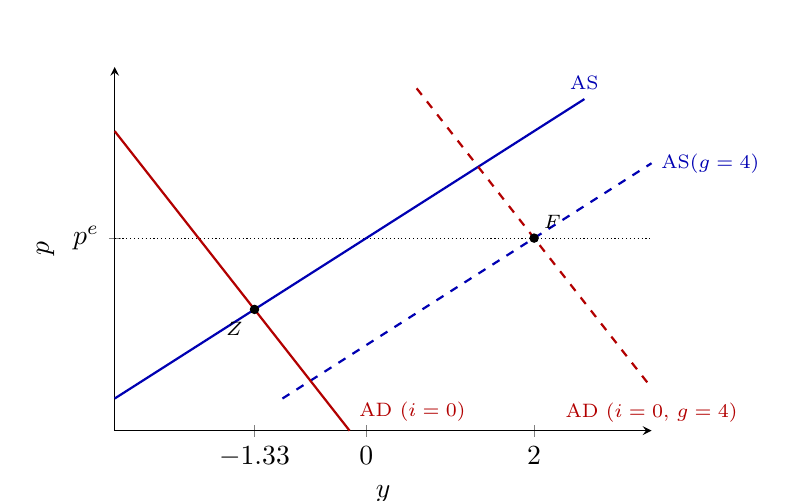
\begin{tikzpicture}
\begin{axis}[width=8.4cm,height=6.2cm,axis lines=left,xmin=-3,xmax=3.4,ymin=-1.8,ymax=1.6,clip=false,
  xlabel={$y$},ylabel={$p$},
  xtick={-1.3333,0,2},xticklabels={$-1.33$,$0$,$2$},ytick={0},yticklabels={$p^e$}]
\addplot[densely dotted,domain=-3:3.4]{0};
\addplot[thick,blue!70!black,domain=-3:2.6]{0.5*x};
\addplot[thick,blue!70!black,dashed,domain=-1:3.4]{0.5*(x-2)};
\addplot[thick,red!70!black,domain=-3:-0.2]{-2-x};
\addplot[thick,red!70!black,dashed,domain=0.6:3.4]{2-x};
\addplot[only marks,mark=*,mark size=1.5pt] coordinates {(-1.3333,-0.6667) (2,0)};
\node[font=\scriptsize,blue!70!black,anchor=south] at (axis cs:2.6,1.3) {AS};
\node[font=\scriptsize,blue!70!black,anchor=west] at (axis cs:3.4,0.7) {AS($g=4$)};
\node[font=\scriptsize,red!70!black,anchor=south west] at (axis cs:-0.2,-1.8) {AD ($i=0$)};
\node[font=\scriptsize,red!70!black,anchor=north] at (axis cs:3.4,-1.45) {AD ($i=0$, $g=4$)};
\node[font=\scriptsize,anchor=north east] at (axis cs:-1.36,-0.70) {$Z$};
\node[font=\scriptsize,anchor=south west] at (axis cs:2,0) {$F$};
\end{axis}
\end{tikzpicture}\\
{\footnotesize $g=4$ shifts AD right by 4 and AS right by $\omega g=2$; the new point $F=(2,\,p^e)$ has
$y=y_n=y_e$.}
\end{center}
\intuicao{Government spending adds demand directly and, by making households work more, adds supply too. When the
central bank is free it leans against the extra demand; stuck at zero it cannot, so more of the spending turns into
output.}
\refbib{Benigno (2015), \S8, eqs.~(22)--(23), Tables~1--2, pp.~514--516; \S9--\S10, pp.~516--521.}
\rubrica{
\item $g$ shifts AD and AS, with $\omega$: 0.15. Moving only AD: $-0.1$.
\item $dy/dg=5/6$ and $d(y-y_e)/dg=1/3$ derived: 0.25 (slip: $-0.1$). Reporting only the output multiplier: max.\ 0.15
on this line.
\item $g=4$ with $y=2$, $p=p^e$: 0.15.
\item Optimal-policy multiplier $\omega=1/2$ with the reason: 0.15.
\item Why larger at the ZLB and the \S10 remark: 0.1. Graph: 0.1.
}
\gap{Prova 01, Q3: which bar moves which curve, the sign of policy, and optimal policy as minimising the loss along AS;
here with a mark-up shock, where $\phi$ does matter, plus the ZLB and fiscal multipliers.}
\end{sol}

\ifsolucoes\else
\vfill
\begin{center}\footnotesize\textit{End of exam.}\end{center}
\fi

\end{document}
